\documentclass{report}

    \usepackage[T1]{fontenc}
    % Nicer default font (+ math font) than Computer Modern for most use cases
    \usepackage{mathpazo}

    % Basic figure setup, for now with no caption control since it's done
    % automatically by Pandoc (which extracts ![](path) syntax from Markdown).
    \usepackage{graphicx}
    % We will generate all images so they have a width \maxwidth. This means
    % that they will get their normal width if they fit onto the page, but
    % are scaled down if they would overflow the margins.
    \makeatletter
    \def\maxwidth{\ifdim\Gin@nat@width>\linewidth\linewidth
    \else\Gin@nat@width\fi}
    \makeatother
    \let\Oldincludegraphics\includegraphics
    % Set max figure width to be 80% of text width, for now hardcoded.
    \renewcommand{\includegraphics}[1]{\Oldincludegraphics[width=.8\maxwidth]{#1}}
    % Ensure that by default, figures have no caption (until we provide a
    % proper Figure object with a Caption API and a way to capture that
    % in the conversion process - todo).
    % \usepackage{caption}
    % \DeclareCaptionLabelFormat{nolabel}{}
    % \captionsetup{labelformat=nolabel}

    \usepackage{adjustbox} % Used to constrain images to a maximum size 
    \usepackage{xcolor} % Allow colors to be defined
    \usepackage{enumerate} % Needed for markdown enumerations to work
    \usepackage{geometry} % Used to adjust the document margins
    \usepackage{amsmath} % Equations
    \usepackage{amssymb} % Equations
    \usepackage{textcomp} % defines textquotesingle
    % Hack from http://tex.stackexchange.com/a/47451/13684:
    \AtBeginDocument{%
        \def\PYZsq{\textquotesingle}% Upright quotes in Pygmentized code
    }
    \usepackage{upquote} % Upright quotes for verbatim code
    \usepackage{eurosym} % defines \euro
    \usepackage[mathletters]{ucs} % Extended unicode (utf-8) support
    \usepackage[utf8x]{inputenc} % Allow utf-8 characters in the tex document
    \usepackage{fancyvrb} % verbatim replacement that allows latex
    \usepackage{grffile} % extends the file name processing of package graphics 
                         % to support a larger range 
    % The hyperref package gives us a pdf with properly built
    % internal navigation ('pdf bookmarks' for the table of contents,
    % internal cross-reference links, web links for URLs, etc.)
    \usepackage{hyperref}
    \usepackage{longtable} % longtable support required by pandoc >1.10
    \usepackage{booktabs}  % table support for pandoc > 1.12.2
    \usepackage[inline]{enumitem} % IRkernel/repr support (it uses the enumerate* environment)
    \usepackage[normalem]{ulem} % ulem is needed to support strikethroughs (\sout)
                                % normalem makes italics be italics, not underlines
    
    \usepackage{ngerman}
    \usepackage{fleqn}
    \usepackage{epsfig}
    \usepackage{a4wide}
    \usepackage{amssymb}
    \usepackage{wasysym}
    \usepackage{stmaryrd}
    \usepackage{color}
    \usepackage{alltt}
    \usepackage{theorem}
    
    \usepackage{hyperref}
    \usepackage[all]{hypcap}
    \hypersetup{
      colorlinks = true, 
      linkcolor  = blue,
      citecolor  = red,
      filecolor  = Gold,
      urlcolor   = [rgb]{0.5, 0.0, 0.5},
      pdfborder  = {0 0 0} 
    }
    
    \usepackage{fancyhdr}
    \usepackage{lastpage} 

    
    % Colors for the hyperref package
    \definecolor{urlcolor}{rgb}{0.5,0,0.5}
    \definecolor{linkcolor}{rgb}{.71,0.21,0.01}
    \definecolor{citecolor}{rgb}{.12,.54,.11}

    % ANSI colors
    \definecolor{ansi-black}{HTML}{3E424D}
    \definecolor{ansi-black-intense}{HTML}{282C36}
    \definecolor{ansi-red}{HTML}{E75C58}
    \definecolor{ansi-red-intense}{HTML}{B22B31}
    \definecolor{ansi-green}{HTML}{00A250}
    \definecolor{ansi-green-intense}{HTML}{007427}
    \definecolor{ansi-yellow}{HTML}{DDB62B}
    \definecolor{ansi-yellow-intense}{HTML}{B27D12}
    \definecolor{ansi-blue}{HTML}{208FFB}
    \definecolor{ansi-blue-intense}{HTML}{0065CA}
    \definecolor{ansi-magenta}{HTML}{D160C4}
    \definecolor{ansi-magenta-intense}{HTML}{A03196}
    \definecolor{ansi-cyan}{HTML}{60C6C8}
    \definecolor{ansi-cyan-intense}{HTML}{258F8F}
    \definecolor{ansi-white}{HTML}{C5C1B4}
    \definecolor{ansi-white-intense}{HTML}{A1A6B2}

    % commands and environments needed by pandoc snippets
    % extracted from the output of `pandoc -s`
    \providecommand{\tightlist}{%
      \setlength{\itemsep}{0pt}\setlength{\parskip}{0pt}}
    \DefineVerbatimEnvironment{Highlighting}{Verbatim}{commandchars=\\\{\}}
    % Add ',fontsize=\small' for more characters per line
    \newenvironment{Shaded}{}{}
    \newcommand{\KeywordTok}[1]{\textcolor[rgb]{0.00,0.44,0.13}{\textbf{{#1}}}}
    \newcommand{\DataTypeTok}[1]{\textcolor[rgb]{0.56,0.13,0.00}{{#1}}}
    \newcommand{\DecValTok}[1]{\textcolor[rgb]{0.25,0.63,0.44}{{#1}}}
    \newcommand{\BaseNTok}[1]{\textcolor[rgb]{0.25,0.63,0.44}{{#1}}}
    \newcommand{\FloatTok}[1]{\textcolor[rgb]{0.25,0.63,0.44}{{#1}}}
    \newcommand{\CharTok}[1]{\textcolor[rgb]{0.25,0.44,0.63}{{#1}}}
    \newcommand{\StringTok}[1]{\textcolor[rgb]{0.25,0.44,0.63}{{#1}}}
    \newcommand{\CommentTok}[1]{\textcolor[rgb]{0.38,0.63,0.69}{\textit{{#1}}}}
    \newcommand{\OtherTok}[1]{\textcolor[rgb]{0.00,0.44,0.13}{{#1}}}
    \newcommand{\AlertTok}[1]{\textcolor[rgb]{1.00,0.00,0.00}{\textbf{{#1}}}}
    \newcommand{\FunctionTok}[1]{\textcolor[rgb]{0.02,0.16,0.49}{{#1}}}
    \newcommand{\RegionMarkerTok}[1]{{#1}}
    \newcommand{\ErrorTok}[1]{\textcolor[rgb]{1.00,0.00,0.00}{\textbf{{#1}}}}
    \newcommand{\NormalTok}[1]{{#1}}
    
    % Additional commands for more recent versions of Pandoc
    \newcommand{\ConstantTok}[1]{\textcolor[rgb]{0.53,0.00,0.00}{{#1}}}
    \newcommand{\SpecialCharTok}[1]{\textcolor[rgb]{0.25,0.44,0.63}{{#1}}}
    \newcommand{\VerbatimStringTok}[1]{\textcolor[rgb]{0.25,0.44,0.63}{{#1}}}
    \newcommand{\SpecialStringTok}[1]{\textcolor[rgb]{0.73,0.40,0.53}{{#1}}}
    \newcommand{\ImportTok}[1]{{#1}}
    \newcommand{\DocumentationTok}[1]{\textcolor[rgb]{0.73,0.13,0.13}{\textit{{#1}}}}
    \newcommand{\AnnotationTok}[1]{\textcolor[rgb]{0.38,0.63,0.69}{\textbf{\textit{{#1}}}}}
    \newcommand{\CommentVarTok}[1]{\textcolor[rgb]{0.38,0.63,0.69}{\textbf{\textit{{#1}}}}}
    \newcommand{\VariableTok}[1]{\textcolor[rgb]{0.10,0.09,0.49}{{#1}}}
    \newcommand{\ControlFlowTok}[1]{\textcolor[rgb]{0.00,0.44,0.13}{\textbf{{#1}}}}
    \newcommand{\OperatorTok}[1]{\textcolor[rgb]{0.40,0.40,0.40}{{#1}}}
    \newcommand{\BuiltInTok}[1]{{#1}}
    \newcommand{\ExtensionTok}[1]{{#1}}
    \newcommand{\PreprocessorTok}[1]{\textcolor[rgb]{0.74,0.48,0.00}{{#1}}}
    \newcommand{\AttributeTok}[1]{\textcolor[rgb]{0.49,0.56,0.16}{{#1}}}
    \newcommand{\InformationTok}[1]{\textcolor[rgb]{0.38,0.63,0.69}{\textbf{\textit{{#1}}}}}
    \newcommand{\WarningTok}[1]{\textcolor[rgb]{0.38,0.63,0.69}{\textbf{\textit{{#1}}}}}
    
    
    % Define a nice break command that doesn't care if a line doesn't already
    % exist.
    \def\br{\hspace*{\fill} \\* }
    % Math Jax compatability definitions
    \def\gt{>}
    \def\lt{<}
    % Document parameters
    \title{Introduction}
    
    % Pygments definitions
    
\makeatletter
\def\PY@reset{\let\PY@it=\relax \let\PY@bf=\relax%
    \let\PY@ul=\relax \let\PY@tc=\relax%
    \let\PY@bc=\relax \let\PY@ff=\relax}
\def\PY@tok#1{\csname PY@tok@#1\endcsname}
\def\PY@toks#1+{\ifx\relax#1\empty\else%
    \PY@tok{#1}\expandafter\PY@toks\fi}
\def\PY@do#1{\PY@bc{\PY@tc{\PY@ul{%
    \PY@it{\PY@bf{\PY@ff{#1}}}}}}}
\def\PY#1#2{\PY@reset\PY@toks#1+\relax+\PY@do{#2}}

\expandafter\def\csname PY@tok@w\endcsname{\def\PY@tc##1{\textcolor[rgb]{0.73,0.73,0.73}{##1}}}
\expandafter\def\csname PY@tok@c\endcsname{\let\PY@it=\textit\def\PY@tc##1{\textcolor[rgb]{0.25,0.50,0.50}{##1}}}
\expandafter\def\csname PY@tok@cp\endcsname{\def\PY@tc##1{\textcolor[rgb]{0.74,0.48,0.00}{##1}}}
\expandafter\def\csname PY@tok@k\endcsname{\let\PY@bf=\textbf\def\PY@tc##1{\textcolor[rgb]{0.00,0.50,0.00}{##1}}}
\expandafter\def\csname PY@tok@kp\endcsname{\def\PY@tc##1{\textcolor[rgb]{0.00,0.50,0.00}{##1}}}
\expandafter\def\csname PY@tok@kt\endcsname{\def\PY@tc##1{\textcolor[rgb]{0.69,0.00,0.25}{##1}}}
\expandafter\def\csname PY@tok@o\endcsname{\def\PY@tc##1{\textcolor[rgb]{0.40,0.40,0.40}{##1}}}
\expandafter\def\csname PY@tok@ow\endcsname{\let\PY@bf=\textbf\def\PY@tc##1{\textcolor[rgb]{0.67,0.13,1.00}{##1}}}
\expandafter\def\csname PY@tok@nb\endcsname{\def\PY@tc##1{\textcolor[rgb]{0.00,0.50,0.00}{##1}}}
\expandafter\def\csname PY@tok@nf\endcsname{\def\PY@tc##1{\textcolor[rgb]{0.00,0.00,1.00}{##1}}}
\expandafter\def\csname PY@tok@nc\endcsname{\let\PY@bf=\textbf\def\PY@tc##1{\textcolor[rgb]{0.00,0.00,1.00}{##1}}}
\expandafter\def\csname PY@tok@nn\endcsname{\let\PY@bf=\textbf\def\PY@tc##1{\textcolor[rgb]{0.00,0.00,1.00}{##1}}}
\expandafter\def\csname PY@tok@ne\endcsname{\let\PY@bf=\textbf\def\PY@tc##1{\textcolor[rgb]{0.82,0.25,0.23}{##1}}}
\expandafter\def\csname PY@tok@nv\endcsname{\def\PY@tc##1{\textcolor[rgb]{0.10,0.09,0.49}{##1}}}
\expandafter\def\csname PY@tok@no\endcsname{\def\PY@tc##1{\textcolor[rgb]{0.53,0.00,0.00}{##1}}}
\expandafter\def\csname PY@tok@nl\endcsname{\def\PY@tc##1{\textcolor[rgb]{0.63,0.63,0.00}{##1}}}
\expandafter\def\csname PY@tok@ni\endcsname{\let\PY@bf=\textbf\def\PY@tc##1{\textcolor[rgb]{0.60,0.60,0.60}{##1}}}
\expandafter\def\csname PY@tok@na\endcsname{\def\PY@tc##1{\textcolor[rgb]{0.49,0.56,0.16}{##1}}}
\expandafter\def\csname PY@tok@nt\endcsname{\let\PY@bf=\textbf\def\PY@tc##1{\textcolor[rgb]{0.00,0.50,0.00}{##1}}}
\expandafter\def\csname PY@tok@nd\endcsname{\def\PY@tc##1{\textcolor[rgb]{0.67,0.13,1.00}{##1}}}
\expandafter\def\csname PY@tok@s\endcsname{\def\PY@tc##1{\textcolor[rgb]{0.73,0.13,0.13}{##1}}}
\expandafter\def\csname PY@tok@sd\endcsname{\let\PY@it=\textit\def\PY@tc##1{\textcolor[rgb]{0.73,0.13,0.13}{##1}}}
\expandafter\def\csname PY@tok@si\endcsname{\let\PY@bf=\textbf\def\PY@tc##1{\textcolor[rgb]{0.73,0.40,0.53}{##1}}}
\expandafter\def\csname PY@tok@se\endcsname{\let\PY@bf=\textbf\def\PY@tc##1{\textcolor[rgb]{0.73,0.40,0.13}{##1}}}
\expandafter\def\csname PY@tok@sr\endcsname{\def\PY@tc##1{\textcolor[rgb]{0.73,0.40,0.53}{##1}}}
\expandafter\def\csname PY@tok@ss\endcsname{\def\PY@tc##1{\textcolor[rgb]{0.10,0.09,0.49}{##1}}}
\expandafter\def\csname PY@tok@sx\endcsname{\def\PY@tc##1{\textcolor[rgb]{0.00,0.50,0.00}{##1}}}
\expandafter\def\csname PY@tok@m\endcsname{\def\PY@tc##1{\textcolor[rgb]{0.40,0.40,0.40}{##1}}}
\expandafter\def\csname PY@tok@gh\endcsname{\let\PY@bf=\textbf\def\PY@tc##1{\textcolor[rgb]{0.00,0.00,0.50}{##1}}}
\expandafter\def\csname PY@tok@gu\endcsname{\let\PY@bf=\textbf\def\PY@tc##1{\textcolor[rgb]{0.50,0.00,0.50}{##1}}}
\expandafter\def\csname PY@tok@gd\endcsname{\def\PY@tc##1{\textcolor[rgb]{0.63,0.00,0.00}{##1}}}
\expandafter\def\csname PY@tok@gi\endcsname{\def\PY@tc##1{\textcolor[rgb]{0.00,0.63,0.00}{##1}}}
\expandafter\def\csname PY@tok@gr\endcsname{\def\PY@tc##1{\textcolor[rgb]{1.00,0.00,0.00}{##1}}}
\expandafter\def\csname PY@tok@ge\endcsname{\let\PY@it=\textit}
\expandafter\def\csname PY@tok@gs\endcsname{\let\PY@bf=\textbf}
\expandafter\def\csname PY@tok@gp\endcsname{\let\PY@bf=\textbf\def\PY@tc##1{\textcolor[rgb]{0.00,0.00,0.50}{##1}}}
\expandafter\def\csname PY@tok@go\endcsname{\def\PY@tc##1{\textcolor[rgb]{0.53,0.53,0.53}{##1}}}
\expandafter\def\csname PY@tok@gt\endcsname{\def\PY@tc##1{\textcolor[rgb]{0.00,0.27,0.87}{##1}}}
\expandafter\def\csname PY@tok@err\endcsname{\def\PY@bc##1{\setlength{\fboxsep}{0pt}\fcolorbox[rgb]{1.00,0.00,0.00}{1,1,1}{\strut ##1}}}
\expandafter\def\csname PY@tok@kc\endcsname{\let\PY@bf=\textbf\def\PY@tc##1{\textcolor[rgb]{0.00,0.50,0.00}{##1}}}
\expandafter\def\csname PY@tok@kd\endcsname{\let\PY@bf=\textbf\def\PY@tc##1{\textcolor[rgb]{0.00,0.50,0.00}{##1}}}
\expandafter\def\csname PY@tok@kn\endcsname{\let\PY@bf=\textbf\def\PY@tc##1{\textcolor[rgb]{0.00,0.50,0.00}{##1}}}
\expandafter\def\csname PY@tok@kr\endcsname{\let\PY@bf=\textbf\def\PY@tc##1{\textcolor[rgb]{0.00,0.50,0.00}{##1}}}
\expandafter\def\csname PY@tok@bp\endcsname{\def\PY@tc##1{\textcolor[rgb]{0.00,0.50,0.00}{##1}}}
\expandafter\def\csname PY@tok@fm\endcsname{\def\PY@tc##1{\textcolor[rgb]{0.00,0.00,1.00}{##1}}}
\expandafter\def\csname PY@tok@vc\endcsname{\def\PY@tc##1{\textcolor[rgb]{0.10,0.09,0.49}{##1}}}
\expandafter\def\csname PY@tok@vg\endcsname{\def\PY@tc##1{\textcolor[rgb]{0.10,0.09,0.49}{##1}}}
\expandafter\def\csname PY@tok@vi\endcsname{\def\PY@tc##1{\textcolor[rgb]{0.10,0.09,0.49}{##1}}}
\expandafter\def\csname PY@tok@vm\endcsname{\def\PY@tc##1{\textcolor[rgb]{0.10,0.09,0.49}{##1}}}
\expandafter\def\csname PY@tok@sa\endcsname{\def\PY@tc##1{\textcolor[rgb]{0.73,0.13,0.13}{##1}}}
\expandafter\def\csname PY@tok@sb\endcsname{\def\PY@tc##1{\textcolor[rgb]{0.73,0.13,0.13}{##1}}}
\expandafter\def\csname PY@tok@sc\endcsname{\def\PY@tc##1{\textcolor[rgb]{0.73,0.13,0.13}{##1}}}
\expandafter\def\csname PY@tok@dl\endcsname{\def\PY@tc##1{\textcolor[rgb]{0.73,0.13,0.13}{##1}}}
\expandafter\def\csname PY@tok@s2\endcsname{\def\PY@tc##1{\textcolor[rgb]{0.73,0.13,0.13}{##1}}}
\expandafter\def\csname PY@tok@sh\endcsname{\def\PY@tc##1{\textcolor[rgb]{0.73,0.13,0.13}{##1}}}
\expandafter\def\csname PY@tok@s1\endcsname{\def\PY@tc##1{\textcolor[rgb]{0.73,0.13,0.13}{##1}}}
\expandafter\def\csname PY@tok@mb\endcsname{\def\PY@tc##1{\textcolor[rgb]{0.40,0.40,0.40}{##1}}}
\expandafter\def\csname PY@tok@mf\endcsname{\def\PY@tc##1{\textcolor[rgb]{0.40,0.40,0.40}{##1}}}
\expandafter\def\csname PY@tok@mh\endcsname{\def\PY@tc##1{\textcolor[rgb]{0.40,0.40,0.40}{##1}}}
\expandafter\def\csname PY@tok@mi\endcsname{\def\PY@tc##1{\textcolor[rgb]{0.40,0.40,0.40}{##1}}}
\expandafter\def\csname PY@tok@il\endcsname{\def\PY@tc##1{\textcolor[rgb]{0.40,0.40,0.40}{##1}}}
\expandafter\def\csname PY@tok@mo\endcsname{\def\PY@tc##1{\textcolor[rgb]{0.40,0.40,0.40}{##1}}}
\expandafter\def\csname PY@tok@ch\endcsname{\let\PY@it=\textit\def\PY@tc##1{\textcolor[rgb]{0.25,0.50,0.50}{##1}}}
\expandafter\def\csname PY@tok@cm\endcsname{\let\PY@it=\textit\def\PY@tc##1{\textcolor[rgb]{0.25,0.50,0.50}{##1}}}
\expandafter\def\csname PY@tok@cpf\endcsname{\let\PY@it=\textit\def\PY@tc##1{\textcolor[rgb]{0.25,0.50,0.50}{##1}}}
\expandafter\def\csname PY@tok@c1\endcsname{\let\PY@it=\textit\def\PY@tc##1{\textcolor[rgb]{0.25,0.50,0.50}{##1}}}
\expandafter\def\csname PY@tok@cs\endcsname{\let\PY@it=\textit\def\PY@tc##1{\textcolor[rgb]{0.25,0.50,0.50}{##1}}}

\def\PYZbs{\char`\\}
\def\PYZus{\char`\_}
\def\PYZob{\char`\{}
\def\PYZcb{\char`\}}
\def\PYZca{\char`\^}
\def\PYZam{\char`\&}
\def\PYZlt{\char`\<}
\def\PYZgt{\char`\>}
\def\PYZsh{\char`\#}
\def\PYZpc{\char`\%}
\def\PYZdl{\char`\$} %$
\def\PYZhy{\char`\-}
\def\PYZsq{\char`\'}
\def\PYZdq{\char`\"}
\def\PYZti{\char`\~}
% for compatibility with earlier versions
\def\PYZat{@}
\def\PYZlb{[}
\def\PYZrb{]}
\makeatother


    % Exact colors from NB
    \definecolor{incolor}{rgb}{0.0, 0.0, 0.5}
    \definecolor{outcolor}{rgb}{0.545, 0.0, 0.0}



    
    % Prevent overflowing lines due to hard-to-break entities
    \sloppy 
    % Setup hyperref package
    \hypersetup{
      breaklinks=true,  % so long urls are correctly broken across lines
      colorlinks=true,
      urlcolor=urlcolor,
      linkcolor=linkcolor,
      citecolor=citecolor,
      }
    % Slightly bigger margins than the latex defaults
    
    \geometry{verbose,tmargin=1in,bmargin=1in,lmargin=1in,rmargin=1in}
    


\renewcommand*{\familydefault}{\sfdefault}

\newcommand{\blue}[1]{{\color{blue}#1}}
\newcommand{\red}[1]{{\color{red}#1}}

\pagestyle{fancy}

\fancyfoot[C]{--- \thepage/\pageref{LastPage}\ ---}

\fancypagestyle{plain}{%
\fancyhf{}
\fancyfoot[C]{--- \thepage/\pageref{LastPage}\ ---}
\renewcommand{\headrulewidth}{0pt}
}

\fancyheadoffset{0.1cm}
\renewcommand{\chaptermark}[1]{\markboth{\chaptername \ \thechapter.\ #1}{}}
\renewcommand{\sectionmark}[1]{\markright{\thesection. \ #1}{}}
\fancyhead[R]{\leftmark}
\fancyhead[L]{\rightmark}

\definecolor{amethyst}{rgb}{1.0, 0.7, 0.4}
\definecolor{orange}{rgb}{1, 0.9, 0.0}

\setlength{\mathindent}{1.3cm}
\setlength{\textwidth}{17cm}
\addtolength{\oddsidemargin}{-1cm}
\addtolength{\evensidemargin}{-1cm}
\addtolength{\topmargin}{-1cm}


\setlength{\mathindent}{1.3cm}
\setlength{\topsep}{0.1cm plus0.1cm minus 0.0cm}
\setlength{\partopsep}{0.0cm plus0.1cm minus 0.0cm}
\setlength{\parsep}{0.1cm plus0.1cm minus 0.0cm}
\setlength{\parskip}{0.1cm plus0.1cm minus 0.0cm}
\newfont{\chess}{chess20}
\newfont{\bigchess}{chess30}
\newcommand{\chf}{\baselineskip20pt\lineskip0pt\chess}
\newcommand{\ds}{\displaystyle}
\newcommand{\diff}{\frac{\textrm{d}\;\;}{\textrm{d}\mbox{$x$}}}

{\theorembodyfont{\slshape}
\newtheorem{Definition}{Definition}
\newtheorem{Notation}[Definition]{Notation}
\newtheorem{Korollar}[Definition]{Korollar}
\newtheorem{Lemma}[Definition]{Lemma}
\newtheorem{Satz}[Definition]{Satz}
\newtheorem{Theorem}[Definition]{Theorem}
}

\hyphenation{com-pre-hen-sion}
% set the monospace-font to Inconsalata-g
% font-source: http://leonardo-m.livejournal.com/77079.html

\title{
\epsfig{file=dhbw-logo.eps, scale=1.5}  \\[0.2cm]
       Theoretical Computer Science \texttt{I}: Logic \\[0.2cm]
      --- Winter 2018 ---     \\[0.3cm]
      DHBW Mannheim}
\author{Prof.~Dr.~Karl Stroetmann}


\date{\today \\[1.0cm]
\begin{minipage}[t]{1.0\linewidth}
\noindent
These lecture notes, the corresponding \LaTeX\ sources and the programs discussed in these lecture notes are available at
\\[0.2cm]
\hspace*{\fill}
\href{https://github.com/karlstroetmann/Logik}{\texttt{https://github.com/karlstroetmann/Logik}}.
\hspace*{\fill} 
\\[0.2cm]
The \href{https://github.com/karlstroetmann/Logik/blob/master/Lecture-Notes-Python/logic.pdf}{lecture notes}
can be found in the dictionary
\href{https://github.com/karlstroetmann/Logik/blob/master/Lecture-Notes-Python}{\texttt{Lecture-Notes-Python}}
in the file \href{https://github.com/karlstroetmann/Logik/blob/master/Lecture-Notes-Python/logic.pdf}{\texttt{logic.pdf}}.
As I am currently switching from using the programming language \href{http://setlx.randoom.org}{\textsc{Setlx}} to using
\href{http://python.org}{\textsl{Python}} instead, these lecture notes are being constantly revised.  At the
moment, the lecture notes still contain \textsc{SetlX} programs.  My goal is to replace these programs with
equivalent \textsl{Python} programs.  In order to automatically update the lecture notes,  you can install
the program \href{http://git-scm.com/download}{\texttt{git}}.  Then, using the command line, you can clone my
repository using the command  
\\[0.2cm]
\hspace*{1.3cm}
\texttt{git clone https://github.com/karlstroetmann/Logik.git}.
\\[0.2cm]
Once the repository has been cloned, it can be updated using the command
\\[0.2cm]
\hspace*{1.3cm}
\texttt{git pull}.
\end{minipage}
}

\newcommand{\quoted}[1]{\texttt{\symbol{34}\texttt{#1}\symbol{34}}}
\newcommand{\schluss}[2]{\frac{\displaystyle\quad \rule[-6pt]{0pt}{12pt}#1 \quad}{\displaystyle\quad \rule{0pt}{10pt}#2 \quad}}
\newcommand{\bruch}[2]{\frac{\displaystyle#1}{\displaystyle #2}}
\newcommand{\vschlus}[1]{{\displaystyle\rule[-6pt]{0pt}{12pt} \atop \rule{0pt}{10pt}#1}}

\newcommand{\example}{\vspace*{0.2cm}

\noindent
\textbf{Beispiel}: \ }

\newcommand{\exampleEng}{\vspace*{0.2cm}

\noindent
\textbf{Example}: \ }

\newcommand{\examples}{\vspace*{0.2cm}

\noindent
\textbf{Beispiele}: \ }

\newcommand{\examplesEng}{\vspace*{0.2cm}

\noindent
\textbf{Examples}: \ }

\newcommand{\next}{\vspace*{0.2cm}

\noindent}

\newcommand{\remark}{\vspace*{0.2cm}

\noindent
\textbf{Bemerkung}: }

\newcommand{\remarks}{

\noindent
\textbf{Bemerkung}: }

\newcommand{\remarkEng}{\vspace*{0.2cm}

\noindent
\textbf{Remark}: }


\newcounter{aufgabe}
\newcommand{\exercise}{\vspace*{0.1cm}
\stepcounter{aufgabe}

\noindent
\textbf{Aufgabe \arabic{aufgabe}}: }

\newcommand{\exerciseEng}{\vspace*{0.1cm}
\stepcounter{aufgabe}

\noindent
\textbf{Exercise \arabic{aufgabe}}: }

\newcommand{\solution}{\vspace*{0.2cm}

\noindent
\textbf{L\"{o}sung}: \ }

\newcommand{\proof}{\vspace*{0.2cm}

\noindent
\textbf{Proof}: }

\newcommand{\lb}{\hspace*{\fill} \linebreak}
\newcommand{\modulo}{\;\texttt{\%}\;}
\newcommand{\qed}{\hspace*{\fill} $\Box$}
\newcommand{\eox}{\hspace*{\fill} $\diamond$}
\newcommand{\exend}{\hspace*{\fill} $\diamond$}
\newcommand{\setl}{\textsc{SetlX}}
\newcommand{\setlx}{\textsc{SetlX}}
\newcommand{\struct}{\mathcal{S}}
\newcommand{\FV}{\textsl{FV}}
\newcommand{\id}{\textrm{id}}
\newcommand{\dom}{\textrm{dom}}
\newcommand{\rng}{\textrm{rng}}
\newcommand{\BV}{\textsl{BV}}
\newcommand{\var}{\textsl{Var}}
\newcommand{\el}{\!\in\!}
\newcommand{\at}{\texttt{\symbol{64}}}
\newcommand{\notel}{\!\not\in\!}
\newcommand{\I}{\mathcal{I}}
\newcommand{\verum}{\top}
\newcommand{\falsum}{\bot}
\newcommand{\gentzen}{\vdash}
\newcommand{\komplement}[1]{\overline{\,#1\,}}
\newcommand{\mathquote}[1]{\mbox{``}\mathtt{#1}\mbox{''}}
\newcommand{\squote}[1]{\symbol{34}\texttt{#1}\symbol{34}}

\newcommand{\circneg}{\mbox{$\bigcirc\hspace*{-0.3cm}\neg$}}
\newcommand{\circwedge}{\mbox{$\bigcirc\hspace*{-0.3cm}\wedge$}}
\newcommand{\circvee}{\mbox{$\bigcirc\hspace*{-0.3cm}\vee$}}
\newcommand{\circright}{\mbox{$\bigcirc\hspace*{-0.45cm}\rightarrow$}}
\newcommand{\circleftright}{\mbox{$\bigcirc\hspace*{-0.45cm}\leftrightarrow$}}
\newcommand{\club }{\ensuremath{\clubsuit   }}
\newcommand{\spade}{\ensuremath{\spadesuit  }}
\newcommand{\heart}{\ensuremath{\heartsuit  }}
\newcommand{\diamo}{\ensuremath{\diamondsuit}}

\newcommand{\hoare}[3]{\bigl\{#1\bigr\}\quad\texttt{#2}\quad\bigl\{#3\bigr\}}
\newcommand{\Oh}{\mathcal{O}}

\newcommand{\myfig}[1]{Abbildung \ref{fig:#1} auf Seite \pageref{fig:#1}}
\newcommand{\myFig}[1]{Figure \ref{fig:#1} on page \pageref{fig:#1}}

\def\pair(#1,#2){\langle #1, #2 \rangle}



\begin{document}
\maketitle
\tableofcontents
\chapter{Introduction}
In this short chapter, I would like to motivate why it is that you have to learn logic when you study computer
science.  After that, I will give a short overview of the lecture.

\section{Motivation}
Modern software systems are among the most complex systems developed by mankind.  You can get a
sense of the complexity of these systems if you look at the amount of work that is necessary to
build and maintain complex software systems.  For example, in the telecommunication industry it is 
quite common that software projects require more than a thousand collaborating developers to 
develop a new system.  Obviously, the failure of a project of this size is very costly.
The page
\\[0.2cm]
\hspace*{1.3cm}
\href{http://spectrum.ieee.org/static/the-staggering-impact-of-it-systems-gone-wrong}{Staggering Impact of IT Systems Gone Wrong} 
\\[0.2cm]
presents a number of examples showing big software projects that have failed and have subsequently caused huge
financial losses.  These examples show that the development of complex software systems requires a high level
of precision and diligence.  Hence, the development of software needs a solid scientific
foundation.  Both \href{https://en.wikipedia.org/wiki/Mathematical_logic}{mathematical logic} and 
\href{https://en.wikipedia.org/wiki/Set_theory}{set theory}
are important parts of this foundation.  Furthermore, both set theory and logic have immediate applications in
computer science. 
\begin{enumerate}
\item Logic can be used to specify the \blue{interfaces} of complex systems.  
\item The correctness of digital circuits can be verified using \blue{automatic theorem provers} that are based on
      propositional logic.
\item Set theory and the theory of relations is one of the foundations of \blue{relational databases}.
\end{enumerate}
It is easy to extend this enumeration.  However, besides their immediate applications, 
there is another reason you have to study both logic and set theory: Without the proper use of
{\color{blue}abstractions}, complex software systems cannot be managed.  After all, nobody is able to keep
millions of lines of program code in her head.  The only way to construct and manage a software system of this
size is to introduce the right abstractions and to develop the system in layers.  Hence, the ability
to work with abstract concepts is one of the main virtues of a modern computer scientist.  
Exposing students to logic and set theory trains their abilities to work with abstract concepts.

From my past teaching experience I know that many students think that a good programmer already is a
good computer scientist.  However, a good programmer need not be a scientist, while a 
{\color{blue}computer \underline{scientist}}, by its very name, is a
{\color{blue}scientist}.  There is no denying that {\color{blue}mathematics} in general and 
{\color{blue}logic} in particular is an important part of science, so you should master it.  Furthermore, this
part of your education is much more permanent than the knowledge of a particular programming
language.  Nobody knows which programming language will be \emph{en vogue} in 10 years from now.  In three
years, when you start your professional career, quite a lot of you will have to learn a new
programming language.  What will count then will be much more your ability to quickly grasp new
concepts rather than your skills in a particular programming language.

\section{Overview} 
The first lecture in theoretical computer science creates the foundation that is needed for future lectures.
This lecture deals mostly with mathematical logic and is structured as follows.
\begin{enumerate}
\item We begin our lecture with a short introduction of set theory.  A basic understanding of set theory is
      necessary for us to formally define the semantics of both propositional logic and first order logic.
\item We proceed to introduce the programming language \textsl{Python}.

      As the concepts introduced in this lecture are quite abstract, it is beneficial to clarify the main
      ideas presented in this lectures via programs.  The programming language
      \href{http://python.org}{\textsl{Python}} supports both sets and their operations and is therefore
      suitable to implement most of the abstract ideas presented in this lecture.  According to the 
      \href{http://ieee.org}{\textsc{Ieee}} (\underline{I}nstitute of \underline{E}lectrical and
      \underline{E}lectronics \underline{E}gineers),  \textsl{Python} is now the 
      \href{https://spectrum.ieee.org/static/interactive-the-top-programming-languages-2018}{most popular programming language}.
      Furthermore, \textsl{Python}
      \href{https://cacm.acm.org/blogs/blog-cacm/176450-python-is-now-the-most-popular-introductory-teaching-language-at-top-u-s-universities/fulltext}{is
        now the most popular introductory teaching language at top U.S. universities}.   For these reasons I
      have decided to base these lectures on \textsl{Python}.

\item Next, we investigate the limits of computability.

      For certain problems there is no algorithm that can solve the problem algorithmically. 
      For example, the question whether a given program will terminate for a given input is not
      \blue{decidable}.  This is known as the \href{https://en.wikipedia.org/wiki/Halting_problem}{halting problem}.  
      We will prove the \blue{undecidability} of the halting problem in the third chapter. 
\item The fourth chapter discusses \href{https://en.wikipedia.org/wiki/Propositional_calculus}{propositional logic}.

      In logic, we distinguish between  \blue{propositional logic},
      \blue{first order logic}, and \blue{higher order logic}.  Propositional logic is only
      concerned with the \blue{logical connectives}
      \\[0.2cm]
      \hspace*{1.3cm}
      ``$\neg$'', ``$\wedge$'', ``$\vee$'', ``$\rightarrow$'' und ``$\leftrightarrow$'',
      \\[0.2cm]
      while first-order logic also investigates the \blue{quantifiers}
      \\[0.2cm]
      \hspace*{1.3cm}
      ``$\forall$'' and ``$\exists$'',
      \\[0.2cm]
      where these quantifiers range over the objects of the \blue{domain of discourse}.
      Finally, in \blue{higher order logic} the quantifiers also range over functions and predicates.

      As propositional logic is easier to grasp than first-order logic, we start our investigation
      of logic with propositional logic.  Furthermore, propositional logic has the advantage of
      being \blue{decidable}:  We will present an algorithm that can check whether a propositional formula
      is universally valid.  In contrast to propositional logic, first-order logic is not decidable.

      Next, we discuss applications of propositional logic:  We will show how the \blue{8 queens problem} 
      can be reduced to the question, whether a formula from propositional logic is satisfiable.  We present
      the algorithm of \blue{Davis and Putnam} that can decide the satisfiability of a propositional formula.
      This algorithm is therefore able to solve the 8 queens problem.  
\item Finally, we discuss \href{https://en.wikipedia.org/wiki/First-order_logic}{first-order logic}.

      The most important concept of the last chapter will be the notion of a \blue{formal proof} in
      first order logic.  To this end, we introduce a \blue{formal proof system} that is
      \blue{complete} for first order logic.  \blue{Completeness} means that we will develop an
      algorithm that can \blue{prove} the correctness of every first-order formula that is
      universally valid.  This algorithm is the foundation of \blue{automated theorem proving}.

      As an application of theorem proving we discuss the systems \href{https://www.cs.unm.edu/~mccune/mace4/}{Prover9} and
      \href{https://www.cs.unm.edu/~mccune/mace4/}{Mace4}. \blue{Prover9} is an automated theorem prover, while
      \blue{Mace4} can be used to refute a mathematical conjecture.
\end{enumerate}

%%% Local Variables: 
%%% mode: latex
%%% TeX-master: "logic"
%%% End: 

\chapter{Naive Set Theory}
The concept of \href{https://en.wikipedia.org/wiki/set_theory}{set theory} has arisen towards the end of the 19th century
from an effort to put mathematics on a solid foundation.  The creation of a solid foundation was considered necessary as
the concept of \emph{infinity} increasingly worried mathematicians. 

The essential parts of set theory have been defined by \href{https://de.wikipedia.org/wiki/Georg_Cantor}{Georg
  Cantor} \index{Cantor, Georg} (1845 -- 1918). The first definition of the concept of a set was approximately as follows
\cite{cantor:1895}: 

\begin{center}
\colorbox{red}{\framebox{\colorbox{yellow}{
\begin{minipage}{0.85\linewidth}
  A ``set'' \index{set} is a \blue{well-defined} collection $M$ of certain objects $x$ of our perception or our thinking.
\end{minipage}}}}
\end{center}
\vspace*{0.2cm}

\noindent
Here, the attribute ``\blue{well-defined}'' expresses the fact that for a given quantity $M$ and an object $x$ we have
to be able to decide whether the object $x$ belongs to the set $M$.  If $x$ belongs to $M$, then $x$ is called an
\blue{element} of the set $M$ and we write this as
\\[0.2cm]
\hspace*{1.3cm}
$x \in M$ \quad (read: $x$ is an element of $M$). 
\\[0.2cm]
Slightly abbreviated we can define the notion of a set as follows: 
\\[0.2cm]
\hspace*{1.3cm}
\textsl{A set is a \blue{well-defined} collection of elements}.
\\[0.2cm]
To mathematically understand the concept of a \blue{well-defined collection of elements},
Cantor introduced the so-called \index{comprehension, axiom of} \blue{axiom of comprehension}.
We can formalize this axiom as follows:  If $p(x)$ a \blue{property} that
an object $x$ can have, we can define the set $M$ of all objects that have this
property.  Therefore, the set $M$ can be defined as 
\\[0.2cm]
\hspace*{1.3cm} 
$M := \{ x \;|\; p(x) \}$ \quad (read: ``$M$ is the set of all those $x$ such that $p(x)$ holds'').
\\[0.2cm]
Here, the property $p(x)$ is just a formula in which the variable $x$ happens to appear.
We illustrate the axiom of comprehension by an example: If $\mathbb{N}$ is
the set of natural numbers, then we can define the set of all \emph{even} natural numbers
via the property \\[0.2cm]
\hspace*{1.3cm} $p(x) \;:=\; (\exists y\in \mathbb{N}: x = 2 \cdot y)$. \\[0.2cm]
Using this property, the set of even natural numbers can be defined as \\[0.2cm]
\hspace*{1.3cm} $\{ x \;|\; \exists y\in \mathbb{N}: x = 2 \cdot y \}$. 

Unfortunately, the unrestricted use of the axiom of comprehension leads to serious problems.  To give an
example, let us consider the property of a set to \underline{not} contain itself.  We define the property
$p(x)$ as
\\[0.2cm]
\hspace*{1.3cm}
 $p(x) := \neg(x \in x)$ 
\\[0.2cm]
and proceed to define the set $R$ as follows
\\[0.2cm]
\hspace*{1.3cm} 
$R := \{ x \;|\; \neg (x \in x) \}$.  
\\[0.2cm]
Intuitively, we might expect that no set can contain itself.  However, things turn out to be more complicated.
Let us try to check whether the set $R$ contains itself.  We have
\\[0.2cm]
\hspace*{1.3cm}
$
\begin{array}{cl}
                  & R \in R \\[0.2cm] 
  \Leftrightarrow & R \in \bigl\{ x \;|\; \neg (x \in x) \bigr\} \\[0.2cm] 
  \Leftrightarrow & \neg (R \in R).
\end{array}
$
\\[0.2cm]
So we have shown that
\\[0.2cm]
\hspace*{1.3cm}
$R \in R \;\Leftrightarrow\; \neg(R \in R)$
\\[0.2cm]
holds.  In other words, the set $R$ is a member of itself if and only if $R$ is not a member of itself!
Obviously, this is a contradiction.  As a way out, we can only conclude that the expression \\[0.2cm]
\hspace*{1.3cm} $\{ x \mid \neg (x \in x) \}$ \\[0.2cm]
\blue{does not define a set}.  This shows that the axiom of comprehension is too general:  Not every expression of the form 
\\[0.2cm] 
\hspace*{1.3cm}
$M := \{ x \mid p(x) \}$ 
\\[0.2cm]
defines a set.  The expression
\\[0.2cm]
\hspace*{1.3cm}
$\bigl\{x \mid \neg(x \in x)\bigr\}$
\\[0.2cm]
has been found by the British logician and philosopher 
\index{Russell, Bertrand}
\href{http://de.wikipedia.org/wiki/Bertrand_Russell}{Bertrand Russell} (1872 -- 1970).  It is known as
\href{http://de.wikipedia.org/wiki/Russellsche_Antinomy}{Russell's Antinomy}. 
\index{Russell's Antinomy, $\{x \mid x \not\in x\}$}

In order to avoid \emph{paradoxes} such as Russell's antinomy, it is necessary to be more careful when sets are
constructed.  In the following, we will present methods to construct sets that are less powerful than the 
axiom of comprehension, but, nevertheless, these methods will be sufficient for our purposes.  We will continue
to use the notation underlying the comprehension axiom and write set definitions in the form
\\[0.2cm]
\hspace*{1.3cm}
$M = \{ x \mid p(x) \}$. \qquad (read: $M$ is the set of all $x$ such that $p(x)$ holds.)  
\\[0.2cm]
However, we won't be allowed to use arbitrary formulas $p(x)$ here.  Instead, the formulas we are going to use
for $p(x)$ have to satisfy some \emph{restrictions}.  These restrictions will prevent the construction of
self-contradictory sets.


\section{Defining Sets by Listing their Elements}
The simplest way to define a set is to list of all of its elements. These elements are enclosed in the
curly braces  ``\texttt{\{}'' and ``\texttt{\}}'' and are separated by commas.
For example, when we define \\[0.2cm]
\hspace*{1.3cm} $M := \{ 1, 2, 3 \}$, \\[0.2cm]
then the set $M$ contains the elements $1$, $2$ and $3$.
Using  the notation of the axiom of comprehension we could write this set as \\[0.2cm]
\hspace*{1.3cm} 
$M = \{ x \mid x = 1 \vee x = 2 \vee x = 3 \}$.
\\[0.2cm]
Another example of a set that can be created by explicitly enumerating its elements
is the set of all lower case Latin characters.  This set is given as
define: \\[0.2cm]
\hspace*{1.3cm} 
$\{\mathtt{a}, \mathtt{b}, \mathtt{c}, \mathtt{d}, \mathtt{e},
 \mathtt{f}, \mathtt{g}, \mathtt{h}, \mathtt{i}, \mathtt{j}, \mathtt{k}, \mathtt{l},
 \mathtt{m}, \mathtt{n}, \mathtt{o}, \mathtt{p}, \mathtt{q}, \mathtt{r}, \mathtt{s},
 \mathtt{t}, \mathtt{u}, \mathtt{v}, \mathtt{w}, \mathtt{x}, \mathtt{y}, \mathtt{z}\}$.
 \\[0.2cm]
Occasionally, we will use \blue{dots notation} to define a set.  Using dots notation, the set of all lower case
elements is written as
\\[0.2cm]
\hspace*{1.3cm}
$\{ \mathtt{a}, \mathtt{b}, \mathtt{c}, \cdots, \mathtt{x}, \mathtt{y}, \mathtt{z}\} $.
\\[0.2cm]
Of course, if we use dots notation the interpretation of the dots ``$\cdots$'' must always be obvious from the
context of the definition. 

As a last example, we consider the \blue{empty set} $\emptyset$, which is defined as
\index{empty set, $\emptyset$}
\\[0.2cm]
\hspace*{1.3cm}
$\emptyset := \{\}$.
\\[0.2cm]
Therefore, the empty set does not contain any element at all.  This set plays an important role in set theory which
is similar to the role played by the number $0$ in algebra.

If a set is defined by listing all of its elements, the order in which the
elements are listed is \blue{not} important.  For example, we have
\\[0.2cm]
\hspace*{1.3cm}
$\{1,2,3\} = \{3,1,2\}$,
\\[0.2cm]
since both sets contain the same elements.   
This is summarized as the statement that 
\\[0.2cm]
\hspace*{1.3cm}
\blue{a set abstracts from the order of its elements}. 


\section{Predefined Infinite Sets of Numbers}
All sets that are defined by explicitly listing their elements can only have finitely many elements.  
In mathematics there are some sets that have an \blue{infinite} number of
elements.  One example is the 
\href{http://en.wikipedia.org/wiki/Natural_number}{set of natural numbers}, \index{set of natural numbers, $\mathbb{N}$} 
which is denoted by the symbol $\mathbb{N}$.
Unlike some other authors, I regard the number zero as a natural number.  This is consistent with the
\href{https://en.wikipedia.org/wiki/ISO_31-11}{\textsc{Iso}-standard 31-11}.\footnote{
  The \textsc{Iso} standard 31-11 has been replaced by the
  \href{https://en.wikipedia.org/wiki/ISO_80000-2}{\textsc{Iso}-standard 80000-2},
  but the definition of the set $\mathbb{N}$ has not changed.  In the text, I did not cite \textsc{Iso} 80000-2 because 
  its content is not freely available, at least not legally.
}
Given the concepts discussed so far, the quantity $\mathbb{N}$ cannot be defined.
We must therefore demand the existence of this set as an \blue{axiom}.  More precisely, we postulate that there is a
set $\mathbb{N}$ which has the following three properties:
\begin{enumerate}
\item $0 \in \mathbb{N}$.
\item If we have a number $n$ such that $n \in \mathbb{N}$, then we also have $n+1 \in \mathbb{N}$.
\item The set $\mathbb{N}$ is the \textbf{smallest} set satisfying the first two conditions.
\end{enumerate}
This is the \blue{inductive definition} of the set of natural numbers.
We write \\[0.2cm]
\hspace*{1.3cm} $\mathbb{N} := \{ 0, 1, 2, 3, \cdots \}$. \\[0.2cm]
Along with the set $\mathbb{N}$ of natural numbers we use the following sets of numbers: 
\begin{enumerate}
\item $\mathbb{N}^*$ is the set of \blue{positive natural numbers}, \index{set of positive natural numbers, $\mathbb{N}^*$} we have
      \\[0.2cm]
      \hspace*{1.3cm}
      $\mathbb{N}^* := \{ n \mid n \in \mathbb{N} \wedge n > 0 \}$.
\item $\mathbb{Z}$ is the set of \blue{integers}, we have
      \index{set of integers, $\mathbb{Z}$}
      \\[0.2cm]
      \hspace*{1.3cm}
      $\mathbb{Z} \ = \{ 0, 1, -1, 2, -2, 3, -3, \cdots \}$ 

\item $\mathbb{Q}$ is the set of \blue{rational numbers}, we have
      \index{set of rational numbers, $\mathbb{Q}$}
      \\[0.2cm]
      \hspace*{1.3cm}
      $\Bigl\{ \ds\frac{\;p\;}{q} \Bigm| p \in \mathbb{Z} \wedge q \in \mathbb{N}^* \Bigr\}$.
\item $\mathbb{R}$ is the set of \blue{real numbers}.  \index{set of real numbers, $\mathbb{R}$}

      This set comprises all numbers that you know from school.  For example, besides the rational numbers,
      this set contains the numbers $\sqrt{2}$ or $\pi$.
      A mathematically clean definition of the notion of a \href{https://en.wikipedia.org/wiki/Real_number}{real number}
      requires a lot of effort and is out of the scope of this lecture.  If you are interested, a detailed
      description of the construction of real numbers is given in my lecture notes on 
      \href{https://github.com/karlstroetmann/Analysis/blob/master/Skript/analysis.pdf}{Analysis}.
\end{enumerate}

\section{The Axiom of Specification}
The \blue{axiom of specification} 
\index{axiom of specification, $\{x \in M \mid p(x) \}$}
(im Deutschen verwenden wir hier den Begriff \blue{Aussonderungs-Axiom}),
\index{Aussonderungs-Axiom}
also known as the 
\href{https://en.wikipedia.org/wiki/Axiom_schema_of_specification}{axiom of restricted comprehension},
is a weakening of the comprehension axiom.  The idea behind the axiom of specification
is to use a property $p$ \blue{to select from an existing set $M$ a subset $N$ of those elements
that have the property $p(x)$}: 
\\[0.2cm]
\hspace*{1.3cm}
$N := \{ x\in M \;|\; p(x) \}$ \qquad (read: $N$ is the set of all $x$ from $M$ that satisfy $p(x)$.)
\\[0.2cm]
Therefore,  the axiom of specification states that if $M$ is a set and $p(x)$ is a property that is either true
or false for elements $x$ of $M$, then 
\\[0.2cm]
\hspace*{1.3cm}
$\{ x\in M \;|\; p(x) \}$ 
\\[0.2cm]
is a set.  In the notation of the axiom of comprehension this set is written as 
\\[0.2cm]
\hspace*{1.3cm}
$N := \{ x \mid x \in M \wedge p(x) \}$. 
\\[0.2cm]
This is a \blue{restricted} form of the axiom of comprehension, because the condition ``$p(x)$'' that was used in the
axiom of comprehension is now strengthened to the condition ``$x \in M \wedge p(x)$''.


\exampleEng
Using the axiom of restricted comprehension, the set of even natural numbers can be defined as 
\\[0.2cm]
\hspace*{1.3cm}
 $\{ x \in \mathbb{N} \;|\; \exists y\in \mathbb{N}: x = 2 \cdot y \}$. 

\exerciseEng
Define the set $S$ of all square numbers, i.e.~the set $S$ should contain the numbers $0$, $1$, $4$, $9$, and
so on.
\eox

\section{Power Sets}
In order to introduce the notion of a \blue{power set} we first have to define the notion of a \blue{subset}.
\index{subset, $A \subseteq B$}
If $M$ and $N$ are sets, then $M$ is a \blue{subset} of $N$ if and only if each element of the
set $M$ is also an element of the set $N$.  In that case, we write $M \subseteq N$.  Formally, we define
 \\[0.2cm]
\hspace*{1.3cm}
$M \subseteq N \;\stackrel{\mathrm{def}}{\Longleftrightarrow}\; \forall x: (x \in M \rightarrow x \in N)$.

\exampleEng
We have
\\[0.2cm]
\hspace*{1.3cm}
$\{ 1, 3, 5\} \subseteq \{ 1, 2, 3, 4, 5 \}$.
\\[0.2cm]
Furthermore, for any set $M$ we have that
\\[0.2cm]
\hspace*{1.3cm}
$\emptyset \subseteq M$. \eox
\vspace*{0.2cm}

The  \blue{power set} (Deutsch: \blue{Potenz-Menge}) of a set $M$ is defined as the set of all subsets of $M$.  
\index{power set, $2^M$} \index{Pozenz-Menge}
This set is written as $2^M$.  Therefore we have
\\[0.2cm] 
\hspace*{1.3cm}
$2^M := \{ x \;|\; x \subseteq M \}$.

\exampleEng
Let us compute the power set of the set $\{1,2,3\}$.  We have \\[0.2cm]
\hspace*{1.3cm}
 $2^{\{1,2,3\}} = \bigl\{ \{\},\, \{1\}, \, \{2\},\, \{3\},\, \{1,2\}, \, \{1,3\}, \{2,3\}, \,\{1,2,3\}\bigr\}$. 
\\[0.2cm]
This set has $8 = 2^3$ elements.  
\eox

In general, if the set $M$ has $m$ different elements, then it can be shown
that the power set $2^M$ has $2^m$ different elements.
More formally, let us designate the number of elements of a finite set $M$ as 
$\textsl{card}(M)$.  Then we have
\\[0.2cm]
\hspace*{1.3cm}
$\textsl{card}\left(2^M\right) = 2^{\textsl{\scriptsize card}(M)}$.
\\[0.2cm]
This explains the notation $2^M$ to denote the power set of $M$.  

\exerciseEng
Compute the set $2^{\{1,2,3,4\}}$.  
\eox

\section{The Union of Sets}
If two sets $M$ and $N$ are given, the \blue{union} (Deutsch: \blue{Vereinigungs-Menge})
\index{union, $A \cup B$} \index{Vereinigungs-Menge}0
of $M$ and $N$ is the set of all elements that are either in the set $M$ or in the set $N$ or in both $M$ and
in $N$.  This set is written as $M \cup N$.
Formally, this set is defined as 
\\[0.2cm]
\hspace*{1.3cm} $M \cup N := \{ x \;|\; x \in M \vee x \in N \}$. 

\exampleEng
If $M = \{1,2,3\}$ and $N = \{2,5\}$, we have 
\\[0.2cm]
\hspace*{1.3cm} 
$\{1,2,3\} \cup \{2,5\} = \{1,2,3,5\}$.  
\\[0.2cm]
Note that $M \cup N$ is written as $\{1,2,3,5\}$  and not as $\{1,2,2,3,3,5\}$.
An object $x$ is either an element of a set or it isn't and hence it does not make sense to list an element
more than once.
\eox
\vspace*{0.2cm}

The concept of the union of two sets can be generalized.  Consider
a set $X$ such that the elements of $X$ are sets themselves. For example, the
\blue{power set} of a set $M$ is a set whose elements are sets themselves.  We can form the union of all the 
sets that are elements of the set $X$.  We write this set as $\bigcup X$.  Formally,
we have
\\[0.2cm]
\hspace*{1.3cm} $\bigcup X := \{ y \;|\; \exists x \in X: y \in x \}$.

\exampleEng
If we have \\[0.2cm]
\hspace*{1.3cm}
 $X = \big\{\, \{\},\, \{1,2\}, \, \{1,3,5\}, \, \{7,4\}\,\big\}$, \\[0.2cm]
then \\[0.2cm] 
\hspace*{1.3cm}
 $\bigcup X = \{ 1, 2, 3, 4, 5, 7 \}$. \eox
\vspace*{0.2cm}

\exerciseEng
Assume that $M$ is a subset of $\mathbb{N}$.  How can the set $\bigcup 2^M$ be written more concisely?
\eox

\section{The Intersection of Sets}
If two sets $M$ and $N$ are given, we define the \blue{intersection} (Deutsch: \blue{Schnitt-Menge}) 
\index{intersection, $A \cap B$} \index{Schnitt-Menge}
of $M$ and $N$ as a set of all objects that are
elements of both $M$ and  $N$.  We write that set as the average $M \cap N$.
Formally, we define 
\\[0.2cm]
\hspace*{1.3cm} $M \cap N := \{ x \mid x \in M \wedge x \in N \}$.

\exampleEng
We calculate the intersection of the sets $M = \{ 1, 3, 5 \}$ and $N = \{ 2, 3, 5, 6 \}$.  We have
\\[0.2cm]
\hspace*{1.3cm} $M \cap N = \{ 3, 5 \}$.
\eox
\vspace*{0.2cm}

The concept of the intersection of two sets can be generalized.  Consider
a set $X$ such that the elements of $X$ are sets themselves. 
We can form the intersection of all the 
sets that are elements of the set $X$.  We write this set as $\bigcap X$.  Formally,
we have
\\[0.2cm]
\hspace*{1.3cm} 
$\bigcap X := \{ y \;|\; \forall x \in X: y \in x \}$.
\vspace*{0.2cm}

\exerciseEng
Assume that $M$ is a subset of $\mathbb{N}$.  How can the set $\bigcap 2^M$ be written more concisely?
\eox

\exerciseEng
The sets $A$ and $B$ are defined as follows. 
\\[0.2cm]
\hspace*{1.3cm}
$A := \{ x \in \mathbb{N} \mid x \modulo 2 = 0 \}$ \quad and \quad
$B := \{ x \in \mathbb{N} \mid x \modulo 3 = 0 \}$.
\\[0.2cm]
(For two natural numbers $x$ and $k$, the notation $x \modulo k$ is used in computer science to denote the
\blue{remainder} that is left when $x$ is divided by $k$.)
How can we write the set $A \cap B$ more concisely?
\eox


\section{The Difference of Sets}
If $M$ and $N$ are sets, we define the \blue{difference}  \index{difference, $A \backslash B$}
(Deutsch: \blue{Differenz-Menge}) \index{Differenz-Menge}
of $M$ and $N$ as the set of all objects from $M$ that are not elements of $N$.  The difference of the sets $M$
and $N$ is written as $M\backslash N$ and is formally defined as
 \\[0.2cm]
\hspace*{1.3cm} $M \backslash N := \{ x \mid x \in M \wedge x \not\in N \}$.

\exampleEng
We compute the difference of the sets $M = \{ 1, 3, 5, 7 \}$ and $N = \{ 2, 3, 5, 6 \}$.  We have
\\[0.2cm]
\hspace*{1.3cm} $M \backslash N = \{ 1, 7 \}$. \eox

\section{Image Sets}
\index{image set, $\{f(x) \mid x \in M\}$}
If $M$ is a set and $f$ is a function defined for all $x$ of $M$, then the \blue{image of $M$ under $f$}
(Deutsch: Bild-Menge) \index{Bild-Menge}
is defined as follows:
\\[0.2cm]
\hspace*{1.3cm}
$f(M) := \{ y \;|\; \exists x \in M: y = f(x) \}$. 
\\[0.2cm]
This set is also written as
\\[0.2cm]
\hspace*{1.3cm}
$f(M) := \bigl\{ f(x) \;|\; x \in M \}$. 

\exampleEng
The set $Q$ of all square numbers can be defined as 
\\[0.2cm]
\hspace*{1.3cm}
$Q := \{ y \mid \exists x \in \mathbb{N}: y = x^2\}$.
\\[0.2cm]
Alternatively, we can define this set as
\\[0.2cm]
\hspace*{1.3cm}
$Q := \bigl\{ x^2 \mid x \in \mathbb{N} \bigr\}$.
\eox

\section{Cartesian Products}
\index{Cartesian product, $A \times B$}
In order to be able to present the notion of a 
\href{https://en.wikipedia.org/wiki/Cartesian_product}{Cartesian product} (Deutsch: \blue{kartesisches Produkt}),
we first have to introduce the notion of an \href{https://en.wikipedia.org/wiki/Ordered_pair}{ordered pair} of two objects
$x$ and $y$.  The \blue{ordered pair} of $x$ and $y$ is written as
\\[0.2cm] 
\hspace*{1.3cm}
$\langle x, y \rangle$.
\\[0.2cm]
In the literature, the ordered pair of $x$ and $y$ is sometimes written as $(x,y)$, but I prefer the notation
using angle brackets.  The  \blue{first component} of the pair $\langle x, y \rangle$ is $x$, while $y$ is
\blue{the second component}.  Two  ordered pairs $\langle x_1, y_1 \rangle$ and $\langle x_2, y_2 \rangle$ are
\blue{equal} if and only if they have the same first and second component, i.e.~we have
\\[0.2cm]
\hspace*{1.3cm}
$\langle x_1, y_1 \rangle \,=\,\langle x_2, y_2 \rangle  \;\Leftrightarrow\; x_1 = x_2 \wedge y_1 = y_2$. 
\\[0.2cm]
The \blue{Cartesian product} of two sets $M$ and $N$ is now defined as the set of all ordered pairs such
that the first component is an element of  $M$ and the second component is an element of $N$.
Formally, we define the cartesian product $M \times N$ of the sets $M$ and $N$ as follows:  
\\[0.2cm]
\hspace*{1.3cm}
$M \times N := \big\{ z \mid \exists x\colon \exists y\colon\bigl(z = \langle x,y\rangle \wedge x\in M \wedge y \in N\bigr) \bigr\}$. 
\\[0.2cm]
To be more concise we usually write this as
\\[0.2cm]
\hspace*{1.3cm}
$M \times N := \big\{ \langle x,y\rangle \mid  x\in M \wedge y \in N \}$.

\exampleEng
If $M = \{ 1, 2, 3 \}$ and $N = \{ 5, 7 \}$ we have
\\[0.2cm]
\hspace*{1.3cm} 
$M \times N = \bigl\{ \pair(1,5),\pair(2,5),\pair(3,5),\pair(1,7),\pair(2,7),\pair(3,7)\bigr\}$.
\eox
\vspace*{0.2cm}

\noindent
The notion of an ordered pair can be generalized to the notion of an
\blue{$n$-tuple} where $n$ is a natural number: An $n$-tuple has the form
\\[0.2cm]
\hspace*{1.3cm} $\langle x_1, x_2, \cdots, x_n \rangle$. 
\\[0.2cm]
In a similar way, we can generalize the notion of a Cartesian product of two sets to the Cartesian product of
$n$ sets.  The \blue{general Cartesian product} of $n$ sets  $M_1$, $\cdots$, $M_n$ is defined as follows: \\[0.2cm]
\hspace*{1.3cm}
$M_1 \times \cdots \times M_n =
  \big\{ \langle x_1,x_2,\cdots,x_n \rangle \bigm| x_1\in M_1 \wedge \cdots \wedge x_n \in M_n \big\}
$. 
\\[0.2cm]
Sometimes,  $n$-tuples are called \blue{lists}.  In this case they are written with the square brackets ``\texttt{[}''
and ``\texttt{]}'' instead of the angle brackets ``$\langle$'' and ``$\rangle$'' that we are using.  

\exerciseEng
Assume that $M$ and $N$ are finite sets.  How can the expression $\textsl{card}(M \times N)$ be reduced to an
expression containing the expressions $\textsl{card}(M)$ and $\textsl{card}(N)$?
\eox

\section{Equality of Sets}
We have now presented all the methods that we will use in this lecture  to construct sets.
Next, we discuss the notion of \blue{equality} of two sets.  As a set is solely defined by its members,
the question of the equality of two sets is governed by the 
\href{https://en.wikipedia.org/wiki/Axiom_of_extensionality}{axiom of extensionality} (Deutsch:
Extensionalitäts-Axiom):
\index{axiom of extensionality,\\ $M = N \;\leftrightarrow\; \forall x: (x \in M \leftrightarrow x \in N)$}
\vspace*{0.2cm}

\begin{center}     
\colorbox{red}{\framebox{\colorbox{yellow}{ 
\begin{minipage}{0.65\linewidth}
{\sl \hspace*{\fill}Two sets are equal if and only if they have the same elements. \hspace*{\fill}}  
\end{minipage}}}}
\end{center}
\vspace{0.2cm}

\noindent
Mathematically, we can write the axiom of extensionality as
\\[0.2cm]
\hspace*{1.3cm} $M = N \;\leftrightarrow\; \forall x: (x \in M \leftrightarrow x \in N)$. 
\\[0.2cm]
An important consequence of this axiom is the fact that the order in which the
elements are listed in a set does not matter.  For example, we have 
\\[0.2cm] 
\hspace*{1.3cm} $\{1,2,3\} = \{3,2,1\}$, 
\\[0.2cm]
because both sets contain the same elements.  Similarly, we have
\\[0.2cm]
\hspace*{1.3cm}
$\{1,2,2,3\} = \{1,1,2,3,3\}$,
\\[0.2cm]
because both these sets contain the elements $1$, $2$, and $3$.  It does not matter how often we list these
elements when defining a set:  An object $x$ either is or is not an element of a given set $M$.  It does not
make sense to say something like ``$M$ contains the object $x$ $n$ times''.\footnote{In the literature, you will find
the concept of a \href{https://en.wikipedia.org/wiki/Multiset}{multiset}.  A \blue{multiset} does not abstract
from the number of occurrences of its elements.  In this lecture, we will not use multisets.}

If two sets are defined by explicitly enumerating their elements, the question whether
these sets are equal is trivial to decide.  However, if a set is defined using the axiom of specification, then
it can be very difficult to decide whether this set is equal to another set.  For 
example, it has been shown that \\[0.2cm]
\hspace*{1.3cm} 
$\{ n \in \mathbb{N}^* \mid \exists x, y, z\in\mathbb{N}^*: x^n + y^n = z^n \} = \{1, 2\}$. 
\\[0.2cm]
However, the proof of this equation is very difficult because this equation
is equivalent to \href{https://en.wikipedia.org/wiki/Fermat%27s_Last_Theorem}{Fermat's conjecture}. 
This conjecture was formulated in 1637 by \href{https://de.wikipedia.org/wiki/Pierre_de_Fermat}{Pierre de Fermat}.  
\index{Fermat's conjecture}
It took mathematicians more than three centuries to come up with a rigorous proof that validates this conjecture:
In 1994 \href{https://de.wikipedia.org/wiki/Andrew_Wiles}{Andrew Wiles}
and \href{https://de.wikipedia.org/wiki/Richard_Taylor_(Mathematician)}{Richard Taylor} were able to do this.
There are some similar conjectures concerning the equality of sets that are still open mathematical problems. 


\section{Chapter Review}
You should be able to answer the following questions without consulting the text.
\begin{enumerate}
\item How have we defined the notion of a set?
\item How is the axiom of comprehension defined?  Why can't we use this axiom to define sets?
\item Explain the axiom of restricted comprehension.
\item Lists all the methods that have been introduced to define sets.
\item Explain the axiom of extensionality.
\end{enumerate}
If you want to develop a deeper understand of set theory, I recommend the book
\\[0.2cm]
\hspace*{1.3cm}
\href{http://www.google.com/search?q=Set+Theory+and+Related+Topics+pdf}{Set Theory and Related Topics} 
\\[0.2cm]
by Seymour Lipschutz \cite{lipschutz:1998}.

%%% Local Variables: 
%%% mode: latex
%%% TeX-master: "logic"
%%% End: 

\chapter{The Programming Language \textsl{Python}}
We have started our lecture with an introduction to set theory.  In my experience, the notions of
set theory are difficult to master for many students because the concepts introduced in set theory
are quite abstract.  Fortunately, there is a programming language that supports sets as a basic data type and
thus enables us to experiment with set theory.  This is the programming language
\href{https://en.wikipedia.org/wiki/Python_(programming_language)}{Python}, which is available at
\href{http://www.python.org}{\texttt{python.org}}. \index{python}
By programming in \textsl{Python}, students can get acquainted with set theory in a playful manner.
Furthermore, as many interesting problems have a straightforward solution as \textsl{Python} programs,
students can appreciate the usefulness of abstract notions from set theory by programming in \textsl{Python}.
According to 
\href{https://cacm.acm.org/blogs/blog-cacm/176450-python-is-now-the-most-popular-introductory-teaching-language-at-top-u-s-universities/fulltext}{Philip Guo},
8 of the top 10 US universities teach \textsl{Python} in their introductory computer science courses.

The easiest way to install python and its libraries is via \href{https://www.anaconda.com/download/}{Anaconda}.
\index{Anaconda}
On many computers, \textsl{Python} is already preinstalled.  Nevertheless, even on those systems it is easiest
to use the \blue{Anaconda} distribution.  The reason is that Anaconda make it very easy to use different
versions of python with different libraries.  In this lecture, we will be using the version 3.8 of \textsl{Python}.

\section{Starting the Interpreter}
My goal is to introduce \textsl{Python} via a number of rather simple examples.  I will present more
advanced features of \textsl{Python} in later sections, but this section is intended to provide a first
impression of the language.


\begin{figure}[!ht]
\centering
\begin{Verbatim}[ frame         = lines, 
                  framesep      = 0.3cm, 
                  firstnumber   = 1,
                  labelposition = bottomline,
                  numbers       = none,
                  numbersep     = -0.2cm,
                  xleftmargin   = 0.0cm,
                  xrightmargin  = 0.0cm,
                ]
    Python 3.6.4 |Anaconda, Inc.| (default, Jan 16 2018, 12:04:33) 
    [GCC 4.2.1 Compatible Clang 4.0.1 (tags/RELEASE_401/final)] on darwin
    Type "help", "copyright", "credits" or "license" for more information.
    >>> 
\end{Verbatim}
\vspace*{-0.3cm}
\caption{The \textsl{Python} welcome message.}
\label{fig:python}
\end{figure}

The language \textsl{Python} is an \blue{interpreted} language.  Hence, there is no need to \blue{compile} a
program.  Instead, \textsl{Python} programs can be executed via the interpreter.  The interpreter is started
by the command:\footnote{
  While I am usually in the habit of terminating every sentence with either a full stop, a question
  mark, or an exclamation mark, I refrain from doing so when the sentence ends in a \textsl{Python} command
  that is shown on a separate line.  The reason is that I want to avoid confusion as it can
  otherwise be hard to understand which part of the line is the command that has to be typed
  verbatim.
}
\\[0.2cm]
\hspace*{1.3cm}
\texttt{python}
\\[0.2cm]
After the interpreter is started, the user sees the output that is shown in Figure 
\ref{fig:python} on page \pageref{fig:python}.  The string
``\texttt{\symbol{62}\symbol{62}\symbol{62}}'' is the \blue{prompt}.  It signals that the interpreter is waiting for input.
If we input the string
\\[0.2cm]
\hspace*{1.3cm}
\texttt{1 + 2}
\\[0.2cm]
and press enter, we get the following output:
\begin{verbatim}
    3
    >>> 
\end{verbatim}
The interpreter has computed the sum $1+2$, returned the result, and prints another prompt waiting
for more input.  Formally, the command ``\texttt{1 + 2}''
is a \blue{script}.  Of course, this is a very small script as it consists only of a single expression.
The command
\\[0.2cm]
\hspace*{1.3cm}
\texttt{exit()}
\\[0.2cm]
terminates the interpreter.   The nice thing about \textsl{Python}  is that we do not need a command line to
execute \textsl{Python} scripts, since we even  can run \textsl{Python} in a
browser in so called \href{https://en.wikipedia.org/wiki/Project_Jupyter}{jupyter notebooks}.  If you have
installed \textsl{Python} by means of the \href{https://www.anaconda.com/download/}{Anaconda} distribution,
then you already have installed these notebooks.  The following subsection contains the \blue{jupyter notebook} 
\href{https://github.com/karlstroetmann/Logic/blob/master/Python/Introduction.ipynb}{\texttt{Introduction.ipynb}}.
You should download this notebook from my github page and try the examples on your own computer.  Of course,
for this to work you first have to install \href{https://jupyter.org}{jupyter}.
\index{jupyter notebook}

\section{\texorpdfstring{An Introduction to
\textsl{Python}}{An Introduction to Python}}\label{an-introduction-to-python}
This \textsl{Python} notebook gives a short introduction to \textsl{Python}.
We will start with the basics but as the main goal of this introduction
is to show how \textsl{Python} supports \blue{sets} we will quickly move
to more advanced topics. In order to show off the features of
\textsl{Python} we will give some examples that are not fully explained at
the point where we introduce them. However, rest assured that they will
be explained eventually.

\subsection{Evaluating expressions}\label{evaluating-expressions}
As Python is an interactive language, expressions can be evaluated
directly. In a \blue{Jupyter} notebook we just have to type Ctrl-Enter
in the cell containing the expression. Instead of Ctrl-Enter we can also
use Shift-Enter.

\begin{Verbatim}[commandchars=\\\{\}]
{\color{incolor}In [{\color{incolor}1}]:} \PY{l+m+mi}{1} \PY{o}{+} \PY{l+m+mi}{2}
\end{Verbatim}

\begin{Verbatim}[commandchars=\\\{\}]
{\color{outcolor}Out[{\color{outcolor}1}]:} 3
\end{Verbatim}
            
In \textsl{Python}, the precision of integers is not bounded. Hence, the
following expression does not cause an overflow.

    \begin{Verbatim}[commandchars=\\\{\}]
{\color{incolor}In[{\color{incolor}2}]:}\PY{l+m+mi}{1}\PY{o}{*}\PY{l+m+mi}{2}\PY{o}{*}\PY{l+m+mi}{3}\PY{o}{*}\PY{l+m+mi}{4}\PY{o}{*}\PY{l+m+mi}{5}\PY{o}{*}\PY{l+m+mi}{6}\PY{o}{*}\PY{l+m+mi}{7}\PY{o}{*}\PY{l+m+mi}{8}\PY{o}{*}\PY{l+m+mi}{9}\PY{o}{*}\PY{l+m+mi}{10}\PY{o}{*}\PY{l+m+mi}{11}\PY{o}{*}\PY{l+m+mi}{12}\PY{o}{*}\PY{l+m+mi}{13}\PY{o}{*}\PY{l+m+mi}{14}\PY{o}{*}\PY{l+m+mi}{15}\PY{o}{*}\PY{l+m+mi}{16}\PY{o}{*}\PY{l+m+mi}{17}\PY{o}{*}\PY{l+m+mi}{18}\PY{o}{*}\PY{l+m+mi}{19}\PY{o}{*}\PY{l+m+mi}{20}\PY{o}{*}\PY{l+m+mi}{21}\PY{o}{*}\PY{l+m+mi}{22}\PY{o}{*}\PY{l+m+mi}{23}\PY{o}{*}\PY{l+m+mi}{24}\PY{o}{*}\PY{l+m+mi}{25}
\end{Verbatim}


\begin{Verbatim}[commandchars=\\\{\}]
{\color{outcolor}Out[{\color{outcolor}2}]:} 15511210043330985984000000
\end{Verbatim}
            
    The next \blue{cell} in this notebook shows how to compute the
\blue{factorial} of 1000, i.e. it shows how to compute the product
\[ 1000! = 1 * 2 * 3 * \cdots * 998 * 999 * 1000 \] It uses some
advanced features from \blue{functional programming} that will be
discussed at a later stage of this introduction.

    \begin{Verbatim}[commandchars=\\\{\}]
{\color{incolor}In [{\color{incolor}3}]:} \PY{k+kn}{import} \PY{n+nn}{functools} 
        
        \PY{n}{functools}\PY{o}{.}\PY{n}{reduce}\PY{p}{(}\PY{k}{lambda} \PY{n}{x}\PY{p}{,} \PY{n}{y}\PY{p}{:} \PY{p}{(}\PY{n}{x}\PY{o}{*}\PY{n}{y}\PY{p}{)}\PY{p}{,} \PY{n+nb}{range}\PY{p}{(}\PY{l+m+mi}{1}\PY{p}{,} \PY{l+m+mi}{1001}\PY{p}{)}\PY{p}{)}
\end{Verbatim}


\begin{Verbatim}[commandchars=\\\{\}]
{\color{outcolor}Out[{\color{outcolor}3}]:}
402387260077093773543702433923003985719374864210714632543799910429938512
398629020592044208486969404800479988610197196058631666872994808558901323
829669944590997424504087073759918823627727188732519779505950995276120874
975462497043601418278094646496291056393887437886487337119181045825783647
849977012476632889835955735432513185323958463075557409114262417474349347
553428646576611667797396668820291207379143853719588249808126867838374559
731746136085379534524221586593201928090878297308431392844403281231558611
036976801357304216168747609675871348312025478589320767169132448426236131
412508780208000261683151027341827977704784635868170164365024153691398281
264810213092761244896359928705114964975419909342221566832572080821333186
116811553615836546984046708975602900950537616475847728421889679646244945
160765353408198901385442487984959953319101723355556602139450399736280750
137837615307127761926849034352625200015888535147331611702103968175921510
907788019393178114194545257223865541461062892187960223838971476088506276
862967146674697562911234082439208160153780889893964518263243671616762179
168909779911903754031274622289988005195444414282012187361745992642956581
746628302955570299024324153181617210465832036786906117260158783520751516
284225540265170483304226143974286933061690897968482590125458327168226458
066526769958652682272807075781391858178889652208164348344825993266043367
660176999612831860788386150279465955131156552036093988180612138558600301
435694527224206344631797460594682573103790084024432438465657245014402821
885252470935190620929023136493273497565513958720559654228749774011413346
962715422845862377387538230483865688976461927383814900140767310446640259
899490222221765904339901886018566526485061799702356193897017860040811889
729918311021171229845901641921068884387121855646124960798722908519296819
372388642614839657382291123125024186649353143970137428531926649875337218
940694281434118520158014123344828015051399694290153483077644569099073152
433278288269864602789864321139083506217095002597389863554277196742822248
757586765752344220207573630569498825087968928162753848863396909959826280
956121450994871701244516461260379029309120889086942028510640182154399457
156805941872748998094254742173582401063677404595741785160829230135358081
840096996372524230560855903700624271243416909004153690105933983835777939
410970027753472000000000000000000000000000000000000000000000000000000000
000000000000000000000000000000000000000000000000000000000000000000000000
000000000000000000000000000000000000000000000000000000000000000000000000
000000000000000000000000000000000000000000000000
\end{Verbatim}
            
The following command will stop the interpreter if executed. It is not
useful inside a \blue{Jupyter} notebook. 
Hence, the next line should not be evaluated. Therefore, I have put a
comment character ``\#'' in the first column of this line.

However, if you do remove the comment character and then evaluate the
line, nothing bad will happen as the interpreter is just restarted by
\blue{Jupyter}.

\begin{Verbatim}[commandchars=\\\{\}]
{\color{incolor}In [{\color{incolor}4}]:} \PY{c+c1}{\PYZsh{} exit()}
\end{Verbatim}

In order to write something to the screen, we can use the function
print. This function can print objects of any type. In the following
example, this function prints a string. In \textsl{Python} any character
sequence enclosed in single quotes is string.

\begin{Verbatim}[commandchars=\\\{\}]
{\color{incolor}In [{\color{incolor}5}]:} \PY{n+nb}{print}\PY{p}{(}\PY{l+s+s1}{\PYZsq{}}\PY{l+s+s1}{Hello, World!}\PY{l+s+s1}{\PYZsq{}}\PY{p}{)}
\end{Verbatim}


\begin{Verbatim}[commandchars=\\\{\}]
Hello, World!
\end{Verbatim}

Instead of using single quotes we can also use double quotes as seen in
the next example.

\begin{Verbatim}[commandchars=\\\{\}]
{\color{incolor}In [{\color{incolor}6}]:} \PY{n+nb}{print}\PY{p}{(}\PY{l+s+s2}{\PYZdq{}}\PY{l+s+s2}{Hello, World!}\PY{l+s+s2}{\PYZdq{}}\PY{p}{)}
\end{Verbatim}


\begin{Verbatim}[commandchars=\\\{\}]
Hello, World!
\end{Verbatim}

The function print accepts any number of arguments. For example, to
print the string
\\[0.2cm]
\hspace*{1.3cm}
"36 * 37 / 2 = "
\\[0.2cm]
followed by the value of the expression \(36 \cdot 37 / 2\) we can use the following print statement:

    \begin{Verbatim}[commandchars=\\\{\}]
{\color{incolor}In [{\color{incolor}7}]:} \PY{n+nb}{print}\PY{p}{(}\PY{l+s+s2}{\PYZdq{}}\PY{l+s+s2}{36 * 37 / 2 =}\PY{l+s+s2}{\PYZdq{}}\PY{p}{,} \PY{l+m+mi}{36} \PY{o}{*} \PY{l+m+mi}{37} \PY{o}{/}\PY{o}{/} \PY{l+m+mi}{2}\PY{p}{)}
\end{Verbatim}

\begin{Verbatim}[commandchars=\\\{\}]
36 * 37 / 2 = 666
\end{Verbatim}

In the expression ``36 * 37 // 2'' we have used the operator ``//'' in order
to enforce \blue{integer division}.  \index{integer division, \texttt{//}}
If we had used the operator ``/''
instead, \textsl{Python} would have used \blue{floating point division}
and therefore would have printed the floating point number 666.0 instead
of the integer 666.

\begin{Verbatim}[commandchars=\\\{\}]
{\color{incolor}In [{\color{incolor}8}]:} \PY{n+nb}{print}\PY{p}{(}\PY{l+s+s2}{\PYZdq{}}\PY{l+s+s2}{36 * 37 / 2 =}\PY{l+s+s2}{\PYZdq{}}\PY{p}{,} \PY{l+m+mi}{36} \PY{o}{*} \PY{l+m+mi}{37} \PY{o}{/} \PY{l+m+mi}{2}\PY{p}{)}
\end{Verbatim}

\begin{Verbatim}[commandchars=\\\{\}]
36 * 37 / 2 = 666.0
\end{Verbatim}

\noindent
The following script reads a natural number \(n\) and computes the sum
\(\sum\limits_{i=1}^n i\).
\begin{enumerate}
\item The function \texttt{input} prompts the user to enter a string.
\item This string is then converted into an integer using the function \texttt{int}.
\item Next, the \blue{set} \texttt{s} is created such that 
      $$\texttt{s} = \{1, \cdots, n\}. $$  
      The set \texttt{s} is constructed using the function \texttt{range}.  A function call 
      of the form $\texttt{range}(a, b + 1)$ returns a \blue{generator} 
      \index{range, $\texttt{range}(a, b+1)$}
      that produces the natural numbers 
      from $a$ to $b$.  By using this generator as an argument to the function \texttt{set}, a set is created 
      that contains all the natural number starting from $a$ upto and including $b$.
      The precise mechanics of \blue{generators} will be explained later.
\item The \texttt{print} statement uses the function \texttt{sum} to add up all the elements of the
      set \texttt{s} and print the resulting sum.
\end{enumerate}

\begin{Verbatim}[commandchars=\\\{\}]
{\color{incolor}In [{\color{incolor}9}]:} \PY{n}{n} \PY{o}{=} \PY{n+nb}{input}\PY{p}{(}\PY{l+s+s1}{\PYZsq{}}\PY{l+s+s1}{Type a natural number and press return: }\PY{l+s+s1}{\PYZsq{}}\PY{p}{)}
        \PY{n}{n} \PY{o}{=} \PY{n+nb}{int}\PY{p}{(}\PY{n}{n}\PY{p}{)}
        \PY{n}{s} \PY{o}{=} \PY{n+nb}{set}\PY{p}{(}\PY{n+nb}{range}\PY{p}{(}\PY{l+m+mi}{1}\PY{p}{,} \PY{n}{n}\PY{o}{+}\PY{l+m+mi}{1}\PY{p}{)}\PY{p}{)}
        \PY{n+nb}{print}\PY{p}{(}\PY{l+s+s1}{\PYZsq{}}\PY{l+s+s1}{The sum 1 + 2 + ... + }\PY{l+s+s1}{\PYZsq{}}\PY{p}{,} \PY{n}{n}\PY{p}{,} \PY{l+s+s1}{\PYZsq{}}\PY{l+s+s1}{ is equal to }\PY{l+s+s1}{\PYZsq{}}\PY{p}{,} \PY{n+nb}{sum}\PY{p}{(}\PY{n}{s}\PY{p}{)}\PY{p}{,} \PY{l+s+s1}{\PYZsq{}}\PY{l+s+s1}{.}\PY{l+s+s1}{\PYZsq{}}\PY{p}{,} \PY{n}{sep}\PY{o}{=} \PY{l+s+s1}{\PYZsq{}}\PY{l+s+s1}{\PYZsq{}}\PY{p}{)}
\end{Verbatim}

\begin{Verbatim}[commandchars=\\\{\}]
Type a natural number and press return: 36
The sum 1 + 2 + {\ldots} + 36 is equal to 666.
\end{Verbatim}

The following example shows how \blue{functions} can be defined in
\textsl{Python}. The function \(\texttt{sum}(n)\) is supposed to compute
the sum of all the numbers in the set \(\{1, \cdots, n\}\). Therefore, we have
 \[\texttt{sum}(n) = \sum\limits_{i=1}^n i. \]
The function sum is defined \blue{recursively}. The recursive
implementation of the function sum can best by understood if we observe
that it satisfies the following two equations:
\begin{enumerate}
\item $\texttt{sum}(0) = 0$, 
\item $\texttt{sum}(n) = \texttt{sum}(n-1) + n \quad$  provided that $n > 0$.
\end{enumerate}

    \begin{Verbatim}[commandchars=\\\{\}]
{\color{incolor}In [{\color{incolor}10}]:} \PY{k}{def} \PY{n+nf}{sum}\PY{p}{(}\PY{n}{n}\PY{p}{)}\PY{p}{:}
             \PY{k}{if} \PY{n}{n} \PY{o}{==} \PY{l+m+mi}{0}\PY{p}{:}
                 \PY{k}{return} \PY{l+m+mi}{0}
             \PY{k}{return} \PY{n+nf}{sum}\PY{p}{(}\PY{n}{n}\PY{o}{\PYZhy{}}\PY{l+m+mi}{1}\PY{p}{)} \PY{o}{+} \PY{n}{n}
\end{Verbatim}
 Let us discuss the implementation of the function sum line by line:

\begin{enumerate}
\item The keyword \texttt{\PY{k}{def}} \index{def, function definition} starts the \blue{definition} of the
      function. 
      It is followed by the \blue{name}
      of the function that is defined.  In this case, the function has the name \texttt{sum}.
      The name is followed by the list of the \blue{parameters} \index{parameter} of the function.  This list is enclosed in
      parentheses. If there is more than one parameter, the parameters have to be separated by commas.
      Finally, there needs to be a colon at the end of the first line. 
\item The \blue{body} of the function is indented.   \textbf{Contrary} to most other programming languages, 
     \textsl{Python} \blue{\underline{is s}p\underline{ace sensitive}} and indentation matters.
    
     The first statement of the body is a \blue{conditional} statement, which starts with the keyword
     \texttt{\PY{k}{if}}.  The keyword is followed by a test.  In this case we test whether the variable $n$ 
     is equal to the number $0$.  Note that this test is followed by a colon.
\item The next line contains a \texttt{\PY{k}{return}} statement.  Note that this statement is again indented.
     All statements indented by the same amount that follow an \texttt{\PY{k}{if}}-statement are considered to be
     the \blue{body} of this \texttt{\PY{k}{if}}-statement, i.e. they get executed if the test of the
     \texttt{\PY{k}{if}}-statement is true.  In this case the body contains only a single statement.

\item The last line of the function definition contains the recursive invocation of the function \texttt{sum}.
\end{enumerate}
Using the function \texttt{sum}, we can compute the sum \(\sum\limits_{i=1}^n i\) for any natural number $n$ 
as follows:
\begin{Verbatim}[commandchars=\\\{\}]
{\color{incolor}In [{\color{incolor}11}]:} \PY{n}{n}     \PY{o}{=} \PY{n+nb}{int}\PY{p}{(}\PY{n+nb}{input}\PY{p}{(}\PY{l+s+s2}{\PYZdq{}}\PY{l+s+s2}{Enter a natural number: }\PY{l+s+s2}{\PYZdq{}}\PY{p}{)}\PY{p}{)}
         \PY{n}{total} \PY{o}{=} \PY{n+nb}{sum}\PY{p}{(}\PY{n}{n}\PY{p}{)}
         \PY{k}{if} \PY{n}{n} \PY{o}{\PYZgt{}} \PY{l+m+mi}{2}\PY{p}{:}
             \PY{n+nb}{print}\PY{p}{(}\PY{l+s+s2}{\PYZdq{}}\PY{l+s+s2}{0 + 1 + 2 + ... + }\PY{l+s+s2}{\PYZdq{}}\PY{p}{,} \PY{n}{n}\PY{p}{,} \PY{l+s+s2}{\PYZdq{}}\PY{l+s+s2}{ = }\PY{l+s+s2}{\PYZdq{}}\PY{p}{,} \PY{n}{total}\PY{p}{,} \PY{n}{sep}\PY{o}{=}\PY{l+s+s1}{\PYZsq{}}\PY{l+s+s1}{\PYZsq{}}\PY{p}{)}
         \PY{k}{else}\PY{p}{:} 
             \PY{n+nb}{print}\PY{p}{(}\PY{n}{total}\PY{p}{)}
\end{Verbatim}


\begin{Verbatim}[commandchars=\\\{\}]
Enter a natural number: 100
0 + 1 + 2 + {\ldots} + 100 = 5050
\end{Verbatim}

\subsection{\texorpdfstring{Sets in
\textsl{Python}}{Sets in Python}}\label{sets-in-python}
\textsl{Python} supports \blue{sets} as a \textbf{native} datatype. This is one of the reasons that have
lead me to choose \textsl{Python} as the programming language for this
course. To get a first impression how sets are handled in \textsl{Python},
let us define two simple sets \(A\) and \(B\) and print them:

\begin{Verbatim}[commandchars=\\\{\}]
{\color{incolor}In [{\color{incolor}12}]:} \PY{n}{A} \PY{o}{=} \PY{p}{\PYZob{}}\PY{l+m+mi}{1}\PY{p}{,} \PY{l+m+mi}{2}\PY{p}{,} \PY{l+m+mi}{3}\PY{p}{\PYZcb{}}
         \PY{n}{B} \PY{o}{=} \PY{p}{\PYZob{}}\PY{l+m+mi}{2}\PY{p}{,} \PY{l+m+mi}{3}\PY{p}{,} \PY{l+m+mi}{4}\PY{p}{\PYZcb{}}
         \PY{n+nb}{print}\PY{p}{(}\PY{l+s+s1}{\PYZsq{}}\PY{l+s+s1}{A = }\PY{l+s+s1}{\PYZsq{}}\PY{p}{,} \PY{n}{A}\PY{p}{,} \PY{l+s+s1}{\PYZsq{}}\PY{l+s+s1}{, B = }\PY{l+s+s1}{\PYZsq{}}\PY{p}{,} \PY{n}{B}\PY{p}{,} \PY{n}{sep}\PY{o}{=}\PY{l+s+s1}{\PYZsq{}}\PY{l+s+s1}{\PYZsq{}}\PY{p}{)}
\end{Verbatim}


\begin{Verbatim}[commandchars=\\\{\}]
A = \{1, 2, 3\}, B = \{2, 3, 4\}
\end{Verbatim}

The last argument \texttt{sep=''} prevents the print statement from separating its arguments with space characters.
When defining the empty set, there is a caveat, as we cannot define the empty set using the
expression \texttt{\{\}}.  The reason is that this expression creates the empty \blue{dictionary} instead. (We will
discuss the data type of \blue{dictionaries} later.) To define the empty set, we therefore have
to use the following expression:

\begin{Verbatim}[commandchars=\\\{\}]
{\color{incolor}In [{\color{incolor}13}]:} \PY{n+nb}{set}\PY{p}{(}\PY{p}{)}
\end{Verbatim}


\begin{Verbatim}[commandchars=\\\{\}]
{\color{outcolor}Out[{\color{outcolor}13}]:} set()
\end{Verbatim}
Note that the empty set is also printed as set() in \textsl{Python} and not as \texttt{\{\}}.
Next, let us compute the union \(A \cup B\). This is done using the
function \texttt{union} or the operator ``\texttt{|}'':

\begin{Verbatim}[commandchars=\\\{\}]
{\color{incolor}In [{\color{incolor}14}]:} \PY{n}{A}\PY{o}{.}\PY{n}{union}\PY{p}{(}\PY{n}{B}\PY{p}{)}
\end{Verbatim}


\begin{Verbatim}[commandchars=\\\{\}]
{\color{outcolor}Out[{\color{outcolor}14}]:} \{1, 2, 3, 4\}
\end{Verbatim}
            
As the function union really acts like a \blue{method}, you might
suspect that it does change its first argument. Fortunately, this is not
the case, \(A\) is unchanged as you can see in the next line:

\begin{Verbatim}[commandchars=\\\{\}]
{\color{incolor}In [{\color{incolor}15}]:} \PY{n}{A}
\end{Verbatim}

\begin{Verbatim}[commandchars=\\\{\}]
{\color{outcolor}Out[{\color{outcolor}15}]:} \{1, 2, 3\}
\end{Verbatim}            
To compute the intersection \(A \cap B\), we use the function \texttt{intersection} or the operator ``\texttt{\&}'':

\begin{Verbatim}[commandchars=\\\{\}]
{\color{incolor}In [{\color{incolor}16}]:} \PY{n}{A}\PY{o}{.}\PY{n}{intersection}\PY{p}{(}\PY{n}{B}\PY{p}{)}
\end{Verbatim}

\begin{Verbatim}[commandchars=\\\{\}]
{\color{outcolor}Out[{\color{outcolor}16}]:} \{2, 3\}
\end{Verbatim}       
Again \(A\) is not changed.

\begin{Verbatim}[commandchars=\\\{\}]
{\color{incolor}In [{\color{incolor}17}]:} \PY{n}{A}
\end{Verbatim}

\begin{Verbatim}[commandchars=\\\{\}]
{\color{outcolor}Out[{\color{outcolor}17}]:} \{1, 2, 3\}
\end{Verbatim}       
The difference \(A \backslash B\) is computed using the operator ``\texttt{-}'':

\begin{Verbatim}[commandchars=\\\{\}]
{\color{incolor}In [{\color{incolor}18}]:} \PY{n}{A} \PY{o}{\PYZhy{}} \PY{n}{B}
\end{Verbatim}

\begin{Verbatim}[commandchars=\\\{\}]
{\color{outcolor}Out[{\color{outcolor}18}]:} \{1\}
\end{Verbatim}           
It is easy to test whether \(A \subseteq B\) holds:

\begin{Verbatim}[commandchars=\\\{\}]
{\color{incolor}In [{\color{incolor}19}]:} \PY{n}{A} \PY{o}{\PYZlt{}}\PY{o}{=} \PY{n}{B}
\end{Verbatim}

\begin{Verbatim}[commandchars=\\\{\}]
{\color{outcolor}Out[{\color{outcolor}19}]:} False
\end{Verbatim}           
Testing whether an object \(x\) is an element of a set \(M\), i.e. to
test, whether \(x \in M\) holds is straightforward:

\begin{Verbatim}[commandchars=\\\{\}]
{\color{incolor}In [{\color{incolor}20}]:} \PY{l+m+mi}{1} \PY{o+ow}{in} \PY{n}{A}
\end{Verbatim}

\begin{Verbatim}[commandchars=\\\{\}]
{\color{outcolor}Out[{\color{outcolor}20}]:} True
\end{Verbatim}          
On the other hand, the number \(1\) is not an element of the set \(B\),
i.e. we have \(1 \not\in B\):

\begin{Verbatim}[commandchars=\\\{\}]
{\color{incolor}In [{\color{incolor}21}]:} \PY{l+m+mi}{1} \PY{o+ow}{not} \PY{o+ow}{in} \PY{n}{B}
\end{Verbatim}


\begin{Verbatim}[commandchars=\\\{\}]
{\color{outcolor}Out[{\color{outcolor}21}]:} True
\end{Verbatim}
            
\subsection{Defining Sets via Selection and
Images}\label{defining-sets-via-selection-and-images}
Remember that we can define subsets of a given set \(M\) via the axiom of
selection. If \(p\) is a property such that for any object \(x\) from
the set \(M\) the expression \(p(x)\) is either True or False, the
subset of all those elements of \(M\) such that \(p(x)\) is True can be
defined as
 \[ \{ x \in M \mid p(x) \}. \] 
For example, if \(M\) is the
set \(\{1, \cdots, 100\}\) and we want to compute the subset of this set
that contains all numbers from \(M\) that are divisible by \(7\), then
this set can be defined as 
\[ \{ x \in M \mid x \;\texttt{\%}\; 7 = 0 \}. \]
In \textsl{Python}, the definition of this set can be given as follows:

    \begin{Verbatim}[commandchars=\\\{\}]
{\color{incolor}In [{\color{incolor}22}]:} \PY{n}{M} \PY{o}{=} \PY{n+nb}{set}\PY{p}{(}\PY{n+nb}{range}\PY{p}{(}\PY{l+m+mi}{1}\PY{p}{,} \PY{l+m+mi}{101}\PY{p}{)}\PY{p}{)}
         \PY{p}{\PYZob{}} \PY{n}{x} \PY{k}{for} \PY{n}{x} \PY{o+ow}{in} \PY{n}{M} \PY{k}{if} \PY{n}{x} \PY{o}{\PYZpc{}} \PY{l+m+mi}{7} \PY{o}{==} \PY{l+m+mi}{0} \PY{p}{\PYZcb{}}
\end{Verbatim}


\begin{Verbatim}[commandchars=\\\{\}]
{\color{outcolor}Out[{\color{outcolor}22}]:} \{7, 14, 21, 28, 35, 42, 49, 56, 63, 70, 77, 84, 91, 98\}
\end{Verbatim}
In general, in \textsl{Python} the set
 \[ \{ x \in M \mid p(x) \} \] 
is computed by the expression 
\[ \{\; x\; \texttt{for}\; x\; \texttt{in}\; M\; \texttt{if}\; p(x)\; \}. \]
\blue{Image} sets can be computed in a similar way. If \(f\) is a
function defined for all elements of a set \(M\), the image set
\[ \{ f(x) \mid x \in M \} \] can be computed in \textsl{Python} as
follows: \[ \{\; f(x)\; \texttt{for}\; x\; \texttt{in}\; M\; \}. \] For
example, the following expression computes the set of all squares of
numbers from the set \(\{1,\cdots,10\}\):

    \begin{Verbatim}[commandchars=\\\{\}]
{\color{incolor}In [{\color{incolor}23}]:} \PY{n}{M} \PY{o}{=} \PY{n+nb}{set}\PY{p}{(}\PY{n+nb}{range}\PY{p}{(}\PY{l+m+mi}{1}\PY{p}{,}\PY{l+m+mi}{11}\PY{p}{)}\PY{p}{)}
         \PY{p}{\PYZob{}} \PY{n}{x}\PY{o}{*}\PY{n}{x} \PY{k}{for} \PY{n}{x} \PY{o+ow}{in} \PY{n}{M} \PY{p}{\PYZcb{}}
\end{Verbatim}


\begin{Verbatim}[commandchars=\\\{\}]
{\color{outcolor}Out[{\color{outcolor}23}]:} \{1, 4, 9, 16, 25, 36, 49, 64, 81, 100\}
\end{Verbatim}
            
The computation of image sets and selections can be combined. If \(M\)
is a set, \(p\) is a property such that \(p(x)\) is either True or False
for elements of \(M\), and \(f\) is a function such that \(f(x)\) is
defined for all \(x \in M\) then we can compute set
\[ \{ f(x) \mid  x \in M \wedge p(x) \} \] of all images \(f(x)\) from
those \(x\in M\) that satisfy the property \(p(x)\) via the expression
\[ \{\; f(x)\; \texttt{for}\; x\; \texttt{in}\; M\; \texttt{if}\; p(x)\; \}. \]
For example, to compute the set of those squares of numbers from the set
\(\{1,\cdots,10\}\) that are even we can write

    \begin{Verbatim}[commandchars=\\\{\}]
{\color{incolor}In [{\color{incolor}24}]:} \PY{n}{M} \PY{o}{=} \PY{n+nb}{set}\PY{p}{(}\PY{n+nb}{range}\PY{p}{(}\PY{l+m+mi}{1}\PY{p}{,}\PY{l+m+mi}{11}\PY{p}{)}\PY{p}{)}
         \PY{p}{\PYZob{}} \PY{n}{x}\PY{o}{*}\PY{n}{x} \PY{k}{for} \PY{n}{x} \PY{o+ow}{in} \PY{n}{M} \PY{k}{if} \PY{n}{x} \PY{o}{\PYZpc{}} \PY{l+m+mi}{2} \PY{o}{==} \PY{l+m+mi}{0} \PY{p}{\PYZcb{}}
\end{Verbatim}


\begin{Verbatim}[commandchars=\\\{\}]
{\color{outcolor}Out[{\color{outcolor}24}]:} \{4, 16, 36, 64, 100\}
\end{Verbatim}
            
We can iterate over more than one set. For example, let us define the
set of all products \(p \cdot q\) of numbers \(p\) and \(q\) from the
set \(\{2, \cdots, 10\}\), i.e.~we intend to define the set
\[ \bigl\{ p \cdot q \bigm| p \in \{2,\cdots,10\} \wedge q \in \{2,\cdots,10\} \bigr\}. \]
In \textsl{Python}, this set is defined as follows:

\begin{Verbatim}[commandchars=\\\{\}]
{\color{incolor}In [{\color{incolor}25}]:} \PY{n+nb}{print}\PY{p}{(}\PY{p}{\PYZob{}} \PY{n}{p} \PY{o}{*} \PY{n}{q} \PY{k}{for} \PY{n}{p} \PY{o+ow}{in} \PY{n+nb}{range}\PY{p}{(}\PY{l+m+mi}{2}\PY{p}{,}\PY{l+m+mi}{11}\PY{p}{)} \PY{k}{for} \PY{n}{q} \PY{o+ow}{in} \PY{n+nb}{range}\PY{p}{(}\PY{l+m+mi}{2}\PY{p}{,}\PY{l+m+mi}{11}\PY{p}{)} \PY{p}{\PYZcb{}}\PY{p}{)}
\end{Verbatim}

\begin{Verbatim}[commandchars=\\\{\}]
\{4, 6, 8, 9, 10, 12, 14, 15, 16, 18, 20, 21, 24, 25, 27, 28, 30, 32, 35,
 36, 40, 42, 45, 48, 49, 50, 54, 56, 60, 63, 64, 70, 72, 80, 81, 90, 100\}
\end{Verbatim}
We can use this set to compute the set of \blue{prime numbers}. 
\index{prime numbers, \\$\{ 2, 3, 5, 7, 11, 13, 17, 19, \cdots\}$}
After all, the set of prime numbers is the set of all those natural numbers
bigger than \(1\) that can not be written as a proper product, that is a
number \(x\) is \blue{prime} if

\begin{enumerate}
\item $x$ is bigger than $1$ and 
\item there are no natural numbers $x$ and $y$ both bigger than $1$ such that $x = p * q$ holds.
\end{enumerate}
More formally, the set \(\mathbb{P}\) of prime numbers is defined as
follows:
\[ \mathbb{P} = \bigl\{ x \in \mathbb{N} \;\bigm|\; x > 1 \wedge \neg \exists p, q \in \mathbb{N}: (x = p \cdot q \wedge p > 1 \wedge q > 1)\bigr\}. \]
Hence the following code computes the set of all primes less than 100:

\begin{Verbatim}[commandchars=\\\{\}]
{\color{incolor}In [{\color{incolor}26}]:} \PY{n}{s} \PY{o}{=} \PY{n+nb}{set}\PY{p}{(}\PY{n+nb}{range}\PY{p}{(}\PY{l+m+mi}{2}\PY{p}{,}\PY{l+m+mi}{100}\PY{p}{)}\PY{p}{)}
         \PY{n+nb}{print}\PY{p}{(}\PY{n}{s} \PY{o}{\PYZhy{}} \PY{p}{\PYZob{}} \PY{n}{p} \PY{o}{*} \PY{n}{q} \PY{k}{for} \PY{n}{p} \PY{o+ow}{in} \PY{n}{s} \PY{k}{for} \PY{n}{q} \PY{o+ow}{in} \PY{n}{s} \PY{p}{\PYZcb{}}\PY{p}{)}
\end{Verbatim}


\begin{Verbatim}[commandchars=\\\{\}]
\{ 2, 3, 5, 7, 11, 13, 17, 19, 23, 29, 31, 37, 41, 43, 47, 53, 59, 61,
  67, 71, 73, 79, 83, 89, 97
\}
\end{Verbatim}
An alternative way to compute primes works by noting that a number \(p\)
is prime iff\footnote{In mathematics it is common to write ``iff'' as an abbreviation for ``if and only if''}
there is no number \(t\) other than \(1\) and \(p\) that
divides the number \(p\). The function dividers given below computes the
set of all numbers dividing a given number \(p\) evenly:

\begin{Verbatim}[commandchars=\\\{\}]
{\color{incolor}In [{\color{incolor}27}]:} \PY{k}{def} \PY{n+nf}{dividers}\PY{p}{(}\PY{n}{p}\PY{p}{)}\PY{p}{:}
             \PY{l+s+s2}{\PYZdq{}}\PY{l+s+s2}{Compute the set of numbers that divide the number p.}\PY{l+s+s2}{\PYZdq{}}
             \PY{k}{return} \PY{p}{\PYZob{}} \PY{n}{t} \PY{k}{for} \PY{n}{t} \PY{o+ow}{in} \PY{n+nb}{range}\PY{p}{(}\PY{l+m+mi}{1}\PY{p}{,} \PY{n}{p}\PY{o}{+}\PY{l+m+mi}{1}\PY{p}{)} \PY{k}{if} \PY{n}{p} \PY{o}{\PYZpc{}} \PY{n}{t} \PY{o}{==} \PY{l+m+mi}{0} \PY{p}{\PYZcb{}}
         
         \PY{n}{n}      \PY{o}{=} \PY{l+m+mi}{100}\PY{p}{;}
         \PY{n}{primes} \PY{o}{=} \PY{p}{\PYZob{}} \PY{n}{p} \PY{k}{for} \PY{n}{p} \PY{o+ow}{in} \PY{n+nb}{range}\PY{p}{(}\PY{l+m+mi}{2}\PY{p}{,} \PY{n}{n}\PY{p}{)} \PY{k}{if} \PY{n}{dividers}\PY{p}{(}\PY{n}{p}\PY{p}{)} \PY{o}{==} \PY{p}{\PYZob{}}\PY{l+m+mi}{1}\PY{p}{,} \PY{n}{p}\PY{p}{\PYZcb{}} \PY{p}{\PYZcb{}}
         \PY{n+nb}{print}\PY{p}{(}\PY{n}{primes}\PY{p}{)}
\end{Verbatim}

\begin{Verbatim}[commandchars=\\\{\}]
\{2,3,5,7,11,13,17,19,23,29,31,37,41,43,47,53,59,61,67,71,73,79,83,89,97\}
\end{Verbatim}

\subsection{Computing the Power Set}\label{computing-the-power-set}
\index{power set, \\ computing the power set in \textsl{Python}}
Unfortunately, there is no operator to compute the power set \(2^M\) of
a given set \(M\). Since the power set is needed frequently, we have to
implement a function \texttt{power} to compute this set ourselves. The easiest
way to compute the power set \(2^M\) of a set \(M\) is to implement the
following recursive equations:
\begin{enumerate}
\item The power set of the empty set contains only the empty set:
    $$2^{\{\}} = \bigl\{\{\}\bigr\}$$
\item If a set $M$ can be written as $M = C \cup \{x\}$, where the element $x$ does not occur in the set $C$, then the power set $2^M$ consists of two sets:
      \begin{itemize}
        \item Firstly, all subsets of $C$ are also subsets of $M$.
        \item Secondly, if A is a subset of $C$, then the set $A \cup\{x\}$ is also a subset of $M$.
      \end{itemize}
    If we combine these parts we get the following equation:
    $$2^{C \cup \{x\}} = 2^C \cup \bigl\{ A \cup \{x\} \bigm| A \in 2^C \bigr\}$$
\end{enumerate}
But there is another problem: In \textsl{Python} we can't create a set
that has elements that are sets themselves! The reason is that in
\textsl{Python} sets are implemented via \blue{hash tables} and therefore
the elements of a set need to be \blue{hashable}.  \index{hashable}
(The notion of an
element being \blue{hashable} will be discussed in more detail in the
lecture on \blue{Algorithms}.) However, sets are \blue{mutable} \index{mutable}, i.e.~sets can be changed,
and \blue{mutable} objects are not \blue{hashable}. Fortunately, there is a
workaround: \textsl{Python} provides the data type of \blue{frozen sets}.
\index{frozen set}
These sets behave like sets but are lacking certain functions that modify sets and
hence are \blue{immutable}. So if we use \blue{frozen sets} as elements of the
power set, we can compute the power set of a given set. The function
\texttt{power} given below shows how this works.

\begin{Verbatim}[commandchars=\\\{\}]
{\color{incolor}In [{\color{incolor}28}]:} \PY{k}{def} \PY{n+nf}{power}\PY{p}{(}\PY{n}{M}\PY{p}{)}\PY{p}{:}
             \PY{l+s+s2}{\PYZdq{}}\PY{l+s+s2}{This function computes the power set of the set M.}\PY{l+s+s2}{\PYZdq{}}
             \PY{k}{if} \PY{n}{M} \PY{o}{==} \PY{n+nb}{set}\PY{p}{(}\PY{p}{)}\PY{p}{:}
                 \PY{k}{return} \PY{p}{\PYZob{}} \PY{n+nb}{frozenset}\PY{p}{(}\PY{p}{)} \PY{p}{\PYZcb{}}
             \PY{k}{else}\PY{p}{:}
                 \PY{n}{C}  \PY{o}{=} \PY{n+nb}{set}\PY{p}{(}\PY{n}{M}\PY{p}{)}  \PY{c+c1}{\PYZsh{} C is a copy of M as we don\PYZsq{}t want to change the set M}
                 \PY{n}{x}  \PY{o}{=} \PY{n}{C}\PY{o}{.}\PY{n}{pop}\PY{p}{(}\PY{p}{)} \PY{c+c1}{\PYZsh{} pop removes an element x from the set C}
                 \PY{n}{P1} \PY{o}{=} \PY{n}{power}\PY{p}{(}\PY{n}{C}\PY{p}{)}
                 \PY{n}{P2} \PY{o}{=} \PY{p}{\PYZob{}} \PY{n}{A}\PY{o}{.}\PY{n}{union}\PY{p}{(}\PY{p}{\PYZob{}}\PY{n}{x}\PY{p}{\PYZcb{}}\PY{p}{)} \PY{k}{for} \PY{n}{A} \PY{o+ow}{in} \PY{n}{P1} \PY{p}{\PYZcb{}}
                 \PY{k}{return} \PY{n}{P1}\PY{o}{.}\PY{n}{union}\PY{p}{(}\PY{n}{P2}\PY{p}{)}
\end{Verbatim}


\begin{Verbatim}[commandchars=\\\{\}]
{\color{incolor}In [{\color{incolor}29}]:} \PY{n}{power}\PY{p}{(}\PY{n}{A}\PY{p}{)}
\end{Verbatim}


\begin{Verbatim}[commandchars=\\\{\}]
{\color{outcolor}Out[{\color{outcolor}29}]:} \{frozenset(),
          frozenset(\{3\}),
          frozenset(\{1\}),
          frozenset(\{2\}),
          frozenset(\{1, 2\}),
          frozenset(\{2, 3\}),
          frozenset(\{1, 3\}),
          frozenset(\{1, 2, 3\})\}
\end{Verbatim}
Let us print this in a more readable way. To this end we implement a
function \texttt{prettify} that turns a set of frozensets into a string that
looks like a set of sets.

\begin{Verbatim}[commandchars=\\\{\}]
{\color{incolor}In [{\color{incolor}30}]:} \PY{k}{def} \PY{n+nf}{prettify}\PY{p}{(}\PY{n}{M}\PY{p}{)}\PY{p}{:}
             \PY{l+s+sd}{\PYZdq{}\PYZdq{}\PYZdq{}Turn the set of frozen sets M into a string that looks like a set of sets.}
         \PY{l+s+sd}{       M is assumed to be the power set of some set.}
         \PY{l+s+sd}{    \PYZdq{}\PYZdq{}\PYZdq{}}
             \PY{n}{result} \PY{o}{=} \PY{l+s+s2}{\PYZdq{}}\PY{l+s+s2}{\PYZob{}\PYZob{}}\PY{l+s+s2}{\PYZcb{}, }\PY{l+s+s2}{\PYZdq{}}   \PY{c+c1}{\PYZsh{} The emepty set is always an element of a power set.}
             \PY{k}{for} \PY{n}{A} \PY{o+ow}{in} \PY{n}{M}\PY{p}{:}
                 \PY{k}{if} \PY{n}{A} \PY{o}{==} \PY{n+nb}{set}\PY{p}{(}\PY{p}{)}\PY{p}{:} \PY{c+c1}{\PYZsh{} The empty set has already been taken care of.}
                     \PY{k}{continue}
                 \PY{n}{result} \PY{o}{+}\PY{o}{=} \PY{n+nb}{str}\PY{p}{(}\PY{n+nb}{set}\PY{p}{(}\PY{n}{A}\PY{p}{)}\PY{p}{)} \PY{o}{+} \PY{l+s+s2}{\PYZdq{}}\PY{l+s+s2}{, }\PY{l+s+s2}{\PYZdq{}} \PY{c+c1}{\PYZsh{} A is converted from a frozen set to a set}
             \PY{n}{result} \PY{o}{=} \PY{n}{result}\PY{p}{[}\PY{p}{:}\PY{o}{\PYZhy{}}\PY{l+m+mi}{2}\PY{p}{]} \PY{c+c1}{\PYZsh{} remove the trailing substring \PYZdq{}, \PYZdq{}}
             \PY{n}{result} \PY{o}{+}\PY{o}{=} \PY{l+s+s2}{\PYZdq{}}\PY{l+s+s2}{\PYZcb{}}\PY{l+s+s2}{\PYZdq{}}
             \PY{k}{return} \PY{n}{result}
\end{Verbatim}


\begin{Verbatim}[commandchars=\\\{\}]
{\color{incolor}In [{\color{incolor}31}]:} \PY{n}{prettify}\PY{p}{(}\PY{n}{power}\PY{p}{(}\PY{n}{A}\PY{p}{)}\PY{p}{)}
\end{Verbatim}


\begin{Verbatim}[commandchars=\\\{\}]
{\color{outcolor}Out[{\color{outcolor}31}]:} '\{\{\}, \{3\}, \{1, 2\}, \{2, 3\}, \{1\}, \{1, 3\}, \{1, 2, 3\}, \{2\}\}'
\end{Verbatim}
            
\subsection{Pairs and Cartesian
Products}\label{pairs-and-cartesian-products}
\index{pairs}
In \textsl{Python}, pairs can be created by enclosing the components of
the pair in parentheses. For example, to compute the pair
\(\langle 1, 2 \rangle\) we can write:

\begin{Verbatim}[commandchars=\\\{\}]
{\color{incolor}In [{\color{incolor}32}]:} \PY{p}{(}\PY{l+m+mi}{1}\PY{p}{,}\PY{l+m+mi}{2}\PY{p}{)}
\end{Verbatim}


\begin{Verbatim}[commandchars=\\\{\}]
{\color{outcolor}Out[{\color{outcolor}32}]:} (1, 2)
\end{Verbatim}
It is not even necessary to enclose the components of a pair in
parentheses. For example, to compute the pair \(\langle 1, 2 \rangle\)
we can use the following expression:

\begin{Verbatim}[commandchars=\\\{\}]
{\color{incolor}In [{\color{incolor}33}]:} \PY{l+m+mi}{1}\PY{p}{,} \PY{l+m+mi}{2}
\end{Verbatim}

\begin{Verbatim}[commandchars=\\\{\}]
{\color{outcolor}Out[{\color{outcolor}33}]:} (1, 2)
\end{Verbatim}
The Cartesian product \(A \times B\) of two sets \(A\) and \(B\) can now
be computed via the following expression:
\[ \{\; (x, y) \;\texttt{for}\; x \;\texttt{in}\; A\; \texttt{for}\; y\; \texttt{in}\; B\; \} \]
For example, as we have defined \(A\) as \(\{1,2,3\}\) and \(B\) as
\(\{2,3,4\}\), the Cartesian product of \(A\) and \(B\) is computed as
follows:

\begin{Verbatim}[commandchars=\\\{\}]
{\color{incolor}In [{\color{incolor}34}]:} \PY{p}{\PYZob{}} \PY{p}{(}\PY{n}{x}\PY{p}{,}\PY{n}{y}\PY{p}{)} \PY{k}{for} \PY{n}{x} \PY{o+ow}{in} \PY{n}{A} \PY{k}{for} \PY{n}{y} \PY{o+ow}{in} \PY{n}{B} \PY{p}{\PYZcb{}}
\end{Verbatim}


\begin{Verbatim}[commandchars=\\\{\}]
{\color{outcolor}Out[{\color{outcolor}34}]:} \{(1, 2), (1, 3), (1, 4), (2, 2), (2, 3), (2, 4), (3, 2), (3, 3), (3, 4)\}
\end{Verbatim}
            
\subsection{Tuples}\label{tuples}
\index{tuple}
The notion of a tuple is a generalization of the notion of a pair. For example, to compute the tuple
\(\langle 1, 2, 3 \rangle\) we can use the following expression:

\begin{Verbatim}[commandchars=\\\{\}]
{\color{incolor}In [{\color{incolor}35}]:} \PY{p}{(}\PY{l+m+mi}{1}\PY{p}{,} \PY{l+m+mi}{2}\PY{p}{,} \PY{l+m+mi}{3}\PY{p}{)}
\end{Verbatim}

\begin{Verbatim}[commandchars=\\\{\}]
{\color{outcolor}Out[{\color{outcolor}35}]:} (1, 2, 3)
\end{Verbatim}
Longer tuples can be build using the function range in combination with the function tuple:

\begin{Verbatim}[commandchars=\\\{\}]
{\color{incolor}In [{\color{incolor}36}]:} \PY{n+nb}{tuple}\PY{p}{(}\PY{n+nb}{range}\PY{p}{(}\PY{l+m+mi}{1}\PY{p}{,} \PY{l+m+mi}{11}\PY{p}{)}\PY{p}{)}
\end{Verbatim}


\begin{Verbatim}[commandchars=\\\{\}]
{\color{outcolor}Out[{\color{outcolor}36}]:} (1, 2, 3, 4, 5, 6, 7, 8, 9, 10)
\end{Verbatim}
Tuples can be \blue{concatenated} using the operator ``\texttt{+}'':

\begin{Verbatim}[commandchars=\\\{\}]
{\color{incolor}In [{\color{incolor}37}]:} \PY{n}{T1} \PY{o}{=} \PY{p}{(}\PY{l+m+mi}{1}\PY{p}{,} \PY{l+m+mi}{2}\PY{p}{,} \PY{l+m+mi}{3}\PY{p}{)}
         \PY{n}{T2} \PY{o}{=} \PY{p}{(}\PY{l+m+mi}{4}\PY{p}{,} \PY{l+m+mi}{5}\PY{p}{,} \PY{l+m+mi}{6}\PY{p}{)}
         \PY{n}{T3} \PY{o}{=} \PY{n}{T1} \PY{o}{+} \PY{n}{T2}
         \PY{n}{T3}
\end{Verbatim}


\begin{Verbatim}[commandchars=\\\{\}]
{\color{outcolor}Out[{\color{outcolor}37}]:} (1, 2, 3, 4, 5, 6)
\end{Verbatim}
The \blue{length} of a tuple is computed using the function \texttt{len}:

\begin{Verbatim}[commandchars=\\\{\}]
{\color{incolor}In [{\color{incolor}38}]:} \PY{n+nb}{len}\PY{p}{(}\PY{n}{T3}\PY{p}{)}
\end{Verbatim}


\begin{Verbatim}[commandchars=\\\{\}]
{\color{outcolor}Out[{\color{outcolor}38}]:} 6
\end{Verbatim}
            
The components of a tuple can be extracted using square brackets. Note
that the first component actually has the index \(0\)! This is similar
to the behaviour of \blue{arrays} in the programming language C.

\begin{Verbatim}[commandchars=\\\{\}]
{\color{incolor}In [{\color{incolor}39}]:} \PY{n+nb}{print}\PY{p}{(}\PY{l+s+s2}{\PYZdq{}}\PY{l+s+s2}{T3[0] =}\PY{l+s+s2}{\PYZdq{}}\PY{p}{,} \PY{n}{T3}\PY{p}{[}\PY{l+m+mi}{0}\PY{p}{]}\PY{p}{)}
         \PY{n+nb}{print}\PY{p}{(}\PY{l+s+s2}{\PYZdq{}}\PY{l+s+s2}{T3[1] =}\PY{l+s+s2}{\PYZdq{}}\PY{p}{,} \PY{n}{T3}\PY{p}{[}\PY{l+m+mi}{1}\PY{p}{]}\PY{p}{)}
         \PY{n+nb}{print}\PY{p}{(}\PY{l+s+s2}{\PYZdq{}}\PY{l+s+s2}{T3[2] =}\PY{l+s+s2}{\PYZdq{}}\PY{p}{,} \PY{n}{T3}\PY{p}{[}\PY{l+m+mi}{2}\PY{p}{]}\PY{p}{)}
\end{Verbatim}

\begin{Verbatim}[commandchars=\\\{\}]
T3[0] = 1
T3[1] = 2
T3[2] = 3
\end{Verbatim}
If we use negative indices, then we index from the back@www of the tuple, as
shown in the following example:

\begin{Verbatim}[commandchars=\\\{\}]
{\color{incolor}In [{\color{incolor}40}]:} \PY{n+nb}{print}\PY{p}{(}\PY{l+s+s2}{\PYZdq{}}\PY{l+s+s2}{T3[\PYZhy{}1] =}\PY{l+s+s2}{\PYZdq{}}\PY{p}{,} \PY{n}{T3}\PY{p}{[}\PY{o}{\PYZhy{}}\PY{l+m+mi}{1}\PY{p}{]}\PY{p}{)} \PY{c+c1}{\PYZsh{} last element}
         \PY{n+nb}{print}\PY{p}{(}\PY{l+s+s2}{\PYZdq{}}\PY{l+s+s2}{T3[\PYZhy{}2] =}\PY{l+s+s2}{\PYZdq{}}\PY{p}{,} \PY{n}{T3}\PY{p}{[}\PY{o}{\PYZhy{}}\PY{l+m+mi}{2}\PY{p}{]}\PY{p}{)} \PY{c+c1}{\PYZsh{} penultimate element}
         \PY{n+nb}{print}\PY{p}{(}\PY{l+s+s2}{\PYZdq{}}\PY{l+s+s2}{T3[\PYZhy{}3] =}\PY{l+s+s2}{\PYZdq{}}\PY{p}{,} \PY{n}{T3}\PY{p}{[}\PY{o}{\PYZhy{}}\PY{l+m+mi}{3}\PY{p}{]}\PY{p}{)} \PY{c+c1}{\PYZsh{} third last element }
\end{Verbatim}

\begin{Verbatim}[commandchars=\\\{\}]
T3[-1] = 6
T3[-2] = 5
T3[-3] = 4
\end{Verbatim}

\begin{Verbatim}[commandchars=\\\{\}]
{\color{incolor}In [{\color{incolor}41}]:} \PY{n}{T3}
\end{Verbatim}

\begin{Verbatim}[commandchars=\\\{\}]
{\color{outcolor}Out[{\color{outcolor}41}]:} (1, 2, 3, 4, 5, 6)
\end{Verbatim}
            
The \blue{slicing} \index{slicing, $L[a:b]$}
operator extracts a subtuple from a given tuple. If
\(L\) is a tuple and \(a\) and \(b\) are natural numbers such that
\(a \leq b\) and \(a,b \in \{0, \texttt{len}(L) \}\), then the syntax of
the slicing operator is as follows: \[ L[a:b] \] The expression
\(L[a:b]\) extracts the subtuple that starts with the element \(L[a]\)
up to and excluding the element \(L[b]\). The following shows an
example:

\begin{Verbatim}[commandchars=\\\{\}]
{\color{incolor}In [{\color{incolor}42}]:} \PY{n}{L} \PY{o}{=} \PY{n+nb}{tuple}\PY{p}{(}\PY{n+nb}{range}\PY{p}{(}\PY{l+m+mi}{1}\PY{p}{,}\PY{l+m+mi}{11}\PY{p}{)}\PY{p}{)}
         \PY{n}{L}\PY{p}{[}\PY{l+m+mi}{2}\PY{p}{:}\PY{l+m+mi}{6}\PY{p}{]}
\end{Verbatim}


\begin{Verbatim}[commandchars=\\\{\}]
{\color{outcolor}Out[{\color{outcolor}42}]:} (3, 4, 5, 6)
\end{Verbatim}
            
Slicing works with negative indices, too:

\begin{Verbatim}[commandchars=\\\{\}]
{\color{incolor}In [{\color{incolor}43}]:} \PY{n}{L}\PY{p}{[}\PY{l+m+mi}{2}\PY{p}{:}\PY{o}{\PYZhy{}}\PY{l+m+mi}{2}\PY{p}{]}
\end{Verbatim}

\begin{Verbatim}[commandchars=\\\{\}]
{\color{outcolor}Out[{\color{outcolor}43}]:} (3, 4, 5, 6, 7, 8)
\end{Verbatim}
If we want to create a tuple of length  $1$, we have to use the following syntax:
\\[0.2cm]
\hspace*{1.3cm}
\texttt{L = (x,)}
\\[0.2cm]
Note that in the expression above the comma is not optional as the expression $(x)$ would be interpreted as 
$x$. 

\subsection{Lists}\label{lists}
\index{list}
Next, we discuss the data type of lists. Lists are a lot like tuples,
but in contrast to tuples, lists are \blue{mutatable}, i.e.~we can
change lists. To construct a list, we use square backets:

\begin{Verbatim}[commandchars=\\\{\}]
{\color{incolor}In [{\color{incolor}44}]:} \PY{n}{L} \PY{o}{=} \PY{p}{[}\PY{l+m+mi}{1}\PY{p}{,}\PY{l+m+mi}{2}\PY{p}{,}\PY{l+m+mi}{3}\PY{p}{]}
         \PY{n}{L}
\end{Verbatim}


\begin{Verbatim}[commandchars=\\\{\}]
{\color{outcolor}Out[{\color{outcolor}44}]:} [1, 2, 3]
\end{Verbatim}
To change the first element of a list, we can use the \blue{index operator}:

\begin{Verbatim}[commandchars=\\\{\}]
{\color{incolor}In [{\color{incolor}45}]:} \PY{n}{L}\PY{p}{[}\PY{l+m+mi}{0}\PY{p}{]} \PY{o}{=} \PY{l+m+mi}{7}
         \PY{n}{L}
\end{Verbatim}

\begin{Verbatim}[commandchars=\\\{\}]
{\color{outcolor}Out[{\color{outcolor}45}]:} [7, 2, 3]
\end{Verbatim}
This last operation would not be possible if L had been a tuple instead
of a list. Lists support concatenation in the same way as tuples:

\begin{Verbatim}[commandchars=\\\{\}]
{\color{incolor}In [{\color{incolor}46}]:} \PY{p}{[}\PY{l+m+mi}{1}\PY{p}{,}\PY{l+m+mi}{2}\PY{p}{,}\PY{l+m+mi}{3}\PY{p}{]} \PY{o}{+} \PY{p}{[}\PY{l+m+mi}{4}\PY{p}{,}\PY{l+m+mi}{5}\PY{p}{,}\PY{l+m+mi}{6}\PY{p}{]}
\end{Verbatim}


\begin{Verbatim}[commandchars=\\\{\}]
{\color{outcolor}Out[{\color{outcolor}46}]:} [1, 2, 3, 4, 5, 6]
\end{Verbatim}
The function \texttt{len} computes the length of a list:

\begin{Verbatim}[commandchars=\\\{\}]
{\color{incolor}In [{\color{incolor}47}]:} \PY{n+nb}{len}\PY{p}{(}\PY{p}{[}\PY{l+m+mi}{4}\PY{p}{,}\PY{l+m+mi}{5}\PY{p}{,}\PY{l+m+mi}{6}\PY{p}{]}\PY{p}{)}
\end{Verbatim}

\begin{Verbatim}[commandchars=\\\{\}]
{\color{outcolor}Out[{\color{outcolor}47}]:} 3
\end{Verbatim}
            
Lists and tuples both support the functions \texttt{max} and \texttt{min}. The expression
\(\texttt{max}(L)\) computes the maximum of all the elements of the list
(or tuple) \(L\), while \(\texttt{min}(L)\) computes the smallest
element of \(L\).

\begin{Verbatim}[commandchars=\\\{\}]
{\color{incolor}In [{\color{incolor}48}]:} \PY{n+nb}{max}\PY{p}{(}\PY{p}{[}\PY{l+m+mi}{1}\PY{p}{,}\PY{l+m+mi}{2}\PY{p}{,}\PY{l+m+mi}{3}\PY{p}{]}\PY{p}{)}
\end{Verbatim}


\begin{Verbatim}[commandchars=\\\{\}]
{\color{outcolor}Out[{\color{outcolor}48}]:} 3
\end{Verbatim}
            
\begin{Verbatim}[commandchars=\\\{\}]
{\color{incolor}In [{\color{incolor}49}]:} \PY{n+nb}{min}\PY{p}{(}\PY{p}{[}\PY{l+m+mi}{1}\PY{p}{,}\PY{l+m+mi}{2}\PY{p}{,}\PY{l+m+mi}{3}\PY{p}{]}\PY{p}{)}
\end{Verbatim}


\begin{Verbatim}[commandchars=\\\{\}]
{\color{outcolor}Out[{\color{outcolor}49}]:} 1
\end{Verbatim}
The functions ``\texttt{min}'' and ``\texttt{max}'' also work for sets.

\subsection{Boolean Operators}\label{boolean-operators}

In \textsl{Python}, the \emph{Boolean} values are written as \texttt{True} and \texttt{False}.

\begin{Verbatim}[commandchars=\\\{\}]
{\color{incolor}In [{\color{incolor}50}]:} \PY{k+kc}{True}
\end{Verbatim}

\begin{Verbatim}[commandchars=\\\{\}]
{\color{outcolor}Out[{\color{outcolor}50}]:} True
\end{Verbatim}
            
\begin{Verbatim}[commandchars=\\\{\}]
{\color{incolor}In [{\color{incolor}51}]:} \PY{k+kc}{False}
\end{Verbatim}

\begin{Verbatim}[commandchars=\\\{\}]
{\color{outcolor}Out[{\color{outcolor}51}]:} False
\end{Verbatim}
            
    These values can be combined using the Boolean operator ``\(\wedge\)'',
``\(\vee\)'', and ``\(\neg\)''. In \textsl{Python}, these operators are denoted as
``\texttt{and}'', ``\texttt{or}'', and ``\texttt{not}''. The following table shows how the operator ``\texttt{and}`` is
defined:

\begin{Verbatim}[commandchars=\\\{\}]
{\color{incolor}In [{\color{incolor}52}]:} \PY{n}{B} \PY{o}{=} \PY{p}{(}\PY{k+kc}{True}\PY{p}{,} \PY{k+kc}{False}\PY{p}{)}
         \PY{k}{for} \PY{n}{x} \PY{o+ow}{in} \PY{n}{B}\PY{p}{:}
             \PY{k}{for} \PY{n}{y} \PY{o+ow}{in} \PY{n}{B}\PY{p}{:}
                 \PY{n+nb}{print}\PY{p}{(}\PY{n}{x}\PY{p}{,} \PY{l+s+s1}{\PYZsq{}}\PY{l+s+s1}{and}\PY{l+s+s1}{\PYZsq{}}\PY{p}{,} \PY{n}{y}\PY{p}{,} \PY{l+s+s1}{\PYZsq{}}\PY{l+s+s1}{=}\PY{l+s+s1}{\PYZsq{}}\PY{p}{,} \PY{n}{x} \PY{o+ow}{and} \PY{n}{y}\PY{p}{)}
\end{Verbatim}

\begin{Verbatim}[commandchars=\\\{\}]
True and True = True
True and False = False
False and True = False
False and False = False
\end{Verbatim}
Next, we show the table for the operator ``\texttt{or}''.
The disjunction of two Boolean values is only \texttt{False} if both values are
\texttt{False}:

\begin{Verbatim}[commandchars=\\\{\}]
{\color{incolor}In [{\color{incolor}53}]:} \PY{k}{for} \PY{n}{x} \PY{o+ow}{in} \PY{n}{B}\PY{p}{:}
             \PY{k}{for} \PY{n}{y} \PY{o+ow}{in} \PY{n}{B}\PY{p}{:}
                 \PY{n+nb}{print}\PY{p}{(}\PY{n}{x}\PY{p}{,} \PY{l+s+s1}{\PYZsq{}}\PY{l+s+s1}{or}\PY{l+s+s1}{\PYZsq{}}\PY{p}{,} \PY{n}{y}\PY{p}{,} \PY{l+s+s1}{\PYZsq{}}\PY{l+s+s1}{=}\PY{l+s+s1}{\PYZsq{}}\PY{p}{,} \PY{n}{x} \PY{o+ow}{or} \PY{n}{y}\PY{p}{)}
\end{Verbatim}


\begin{Verbatim}[commandchars=\\\{\}]
True or True = True
True or False = True
False or True = True
False or False = False
\end{Verbatim}
Finally, the negation operator ``\texttt{not}'' works as expected:

\begin{Verbatim}[commandchars=\\\{\}]
{\color{incolor}In [{\color{incolor}54}]:} \PY{k}{for} \PY{n}{x} \PY{o+ow}{in} \PY{n}{B}\PY{p}{:}
             \PY{n+nb}{print}\PY{p}{(}\PY{l+s+s1}{\PYZsq{}}\PY{l+s+s1}{not}\PY{l+s+s1}{\PYZsq{}}\PY{p}{,} \PY{n}{x}\PY{p}{,} \PY{l+s+s1}{\PYZsq{}}\PY{l+s+s1}{=}\PY{l+s+s1}{\PYZsq{}}\PY{p}{,} \PY{o+ow}{not} \PY{n}{x}\PY{p}{)}
\end{Verbatim}

\begin{Verbatim}[commandchars=\\\{\}]
not True = False
not False = True
\end{Verbatim}
Boolean values are created by comparing numbers using the following comparison operators:
\begin{enumerate}
\item $a\;\texttt{==}\;b$ is true iff $a$ is equal to $b$.
\item $a\;\texttt{!=}\;b$ is true iff $a$ is different from $b$.
\item $a\;\texttt{<}\;b$ is true iff $a$ is less than $b$.
\item $a\;\texttt{<=}\;b$ is true iff $a$ is less than or equal to $b$.
\item $a\;\texttt{>=}\;b$ is true iff $a$ is bigger than or equal to $b$.
\item $a\;\texttt{>}\;b$ is true iff $a$ is bigger than $b$.
\end{enumerate}

\begin{Verbatim}[commandchars=\\\{\}]
{\color{incolor}In [{\color{incolor}55}]:} \PY{l+m+mi}{1} \PY{o}{==} \PY{l+m+mi}{2}
\end{Verbatim}


\begin{Verbatim}[commandchars=\\\{\}]
{\color{outcolor}Out[{\color{outcolor}55}]:} False
\end{Verbatim}
            
\begin{Verbatim}[commandchars=\\\{\}]
{\color{incolor}In [{\color{incolor}56}]:} \PY{l+m+mi}{1} \PY{o}{\PYZlt{}} \PY{l+m+mi}{2}
\end{Verbatim}


\begin{Verbatim}[commandchars=\\\{\}]
{\color{outcolor}Out[{\color{outcolor}56}]:} True
\end{Verbatim}
            
\begin{Verbatim}[commandchars=\\\{\}]
{\color{incolor}In [{\color{incolor}57}]:} \PY{l+m+mi}{1} \PY{o}{\PYZlt{}}\PY{o}{=} \PY{l+m+mi}{2}
\end{Verbatim}


\begin{Verbatim}[commandchars=\\\{\}]
{\color{outcolor}Out[{\color{outcolor}57}]:} True
\end{Verbatim}
            
\begin{Verbatim}[commandchars=\\\{\}]
{\color{incolor}In [{\color{incolor}58}]:} \PY{l+m+mi}{1} \PY{o}{\PYZgt{}} \PY{l+m+mi}{2}
\end{Verbatim}


\begin{Verbatim}[commandchars=\\\{\}]
{\color{outcolor}Out[{\color{outcolor}58}]:} False
\end{Verbatim}
            
\begin{Verbatim}[commandchars=\\\{\}]
{\color{incolor}In [{\color{incolor}59}]:} \PY{l+m+mi}{1} \PY{o}{\PYZgt{}}\PY{o}{=} \PY{l+m+mi}{2}
\end{Verbatim}


\begin{Verbatim}[commandchars=\\\{\}]
{\color{outcolor}Out[{\color{outcolor}59}]:} False
\end{Verbatim}
Comparison operators can be \blue{chained} as shown in the following example:

\begin{Verbatim}[commandchars=\\\{\}]
{\color{incolor}In [{\color{incolor}60}]:} \PY{l+m+mi}{1} \PY{o}{\PYZlt{}} \PY{l+m+mi}{2} \PY{o}{\PYZlt{}} \PY{l+m+mi}{3}
\end{Verbatim}


\begin{Verbatim}[commandchars=\\\{\}]
{\color{outcolor}Out[{\color{outcolor}60}]:} True
\end{Verbatim}
            
\textsl{Python} supports the \blue{universal quantifier} \(\forall\) (read: \emph{for all}). If \(L\) is
a list of Boolean values, then we can check whether all elements of
\(L\) are true by writing \[ \texttt{all}(L) \] For example, to check
whether all elements of a list \(L\) are even we can write the
following:

\begin{Verbatim}[commandchars=\\\{\}]
{\color{incolor}In [{\color{incolor}61}]:} \PY{n}{L} \PY{o}{=} \PY{p}{[}\PY{l+m+mi}{2}\PY{p}{,} \PY{l+m+mi}{4}\PY{p}{,} \PY{l+m+mi}{6}\PY{p}{]}
         \PY{n+nb}{all}\PY{p}{(}\PY{p}{[}\PY{n}{x} \PY{o}{\PYZpc{}} \PY{l+m+mi}{2} \PY{o}{==} \PY{l+m+mi}{0} \PY{k}{for} \PY{n}{x} \PY{o+ow}{in} \PY{n}{L}\PY{p}{]}\PY{p}{)}
\end{Verbatim}


\begin{Verbatim}[commandchars=\\\{\}]
{\color{outcolor}Out[{\color{outcolor}61}]:} True
\end{Verbatim}
            
    \subsection{Control Structures}\label{control-structures}

    First of all, \textsl{Python} supports \emph{branching} statements. The following
example is taken from the \textsl{Python} tutorial at \href{https://python.org}{https://python.org}:

\begin{Verbatim}[commandchars=\\\{\}]
{\color{incolor}In [{\color{incolor}62}]:} \PY{n}{x} \PY{o}{=} \PY{n+nb}{int}\PY{p}{(}\PY{n+nb}{input}\PY{p}{(}\PY{l+s+s2}{\PYZdq{}}\PY{l+s+s2}{Please enter an integer: }\PY{l+s+s2}{\PYZdq{}}\PY{p}{)}\PY{p}{)}
         \PY{k}{if} \PY{n}{x} \PY{o}{\PYZlt{}} \PY{l+m+mi}{0}\PY{p}{:}
            \PY{n+nb}{print}\PY{p}{(}\PY{l+s+s1}{\PYZsq{}}\PY{l+s+s1}{The number is negative!}\PY{l+s+s1}{\PYZsq{}}\PY{p}{)}
         \PY{k}{elif} \PY{n}{x} \PY{o}{==} \PY{l+m+mi}{0}\PY{p}{:}
            \PY{n+nb}{print}\PY{p}{(}\PY{l+s+s1}{\PYZsq{}}\PY{l+s+s1}{The number is zero.}\PY{l+s+s1}{\PYZsq{}}\PY{p}{)}
         \PY{k}{elif} \PY{n}{x} \PY{o}{==} \PY{l+m+mi}{1}\PY{p}{:}
            \PY{n+nb}{print}\PY{p}{(}\PY{l+s+s2}{\PYZdq{}}\PY{l+s+s2}{It}\PY{l+s+s2}{\PYZsq{}}\PY{l+s+s2}{s a one.}\PY{l+s+s2}{\PYZdq{}}\PY{p}{)}
         \PY{k}{else}\PY{p}{:}
            \PY{n+nb}{print}\PY{p}{(}\PY{l+s+s2}{\PYZdq{}}\PY{l+s+s2}{It}\PY{l+s+s2}{\PYZsq{}}\PY{l+s+s2}{s more than one.}\PY{l+s+s2}{\PYZdq{}}\PY{p}{)}
\end{Verbatim}

\begin{Verbatim}[commandchars=\\\{\}]
Please enter an integer: 42
It's more than one.
\end{Verbatim}
\blue{Loops} can be used to iterate over sets, lists, tuples, or
generators. The following example prints the numbers from 1 to 10.
\index{loop} \index{for}

\begin{Verbatim}[commandchars=\\\{\}]
{\color{incolor}In [{\color{incolor}63}]:} \PY{k}{for} \PY{n}{x} \PY{o+ow}{in} \PY{n+nb}{range}\PY{p}{(}\PY{l+m+mi}{1}\PY{p}{,} \PY{l+m+mi}{11}\PY{p}{)}\PY{p}{:}
             \PY{n+nb}{print}\PY{p}{(}\PY{n}{x}\PY{p}{)}
\end{Verbatim}


\begin{Verbatim}[commandchars=\\\{\}]
1
2
3
4
5
6
7
8
9
10
\end{Verbatim}
The same can be achieved with a \texttt{while} loop:
\index{while}

\begin{Verbatim}[commandchars=\\\{\}]
{\color{incolor}In [{\color{incolor}64}]:} \PY{n}{x} \PY{o}{=} \PY{l+m+mi}{1}
         \PY{k}{while} \PY{n}{x} \PY{o}{\PYZlt{}}\PY{o}{=} \PY{l+m+mi}{7}\PY{p}{:}
             \PY{n+nb}{print}\PY{p}{(}\PY{n}{x}\PY{p}{)}
             \PY{n}{x} \PY{o}{+}\PY{o}{=} \PY{l+m+mi}{1}
\end{Verbatim}


\begin{Verbatim}[commandchars=\\\{\}]
1
2
3
4
5
6
7
\end{Verbatim}
The following program computes the prime numbers according to an
algorithm given by  \href{https://en.wikipedia.org/wiki/Eratosthenes}{(Eratosthenes of Cyrene, 276 BC -- 195/194 BC)}.
\index{Eratosthenes of Cyrene}

\begin{enumerate}
\item We set $n$ equal to 100 as we want to compute the set all prime numbers less or equal that 100.
\item \texttt{primes} is the list of numbers from 0 upto $n$, i.e.~we have initially
      $$ \texttt{primes} = [0,1,2,\cdots,n] $$
      Therefore, we have
      $$ \texttt{primes}[i] = i \quad \mbox{for all $i \in \{0,1,\cdots,n\}$.} $$
      The idea is to set \texttt{primes[$i$]} to zero iff $i$ is a proper product of two numbers.

\item To this end we iterate over all $i$ and $j$ from the set $\{2,\cdots,n\}$
  and set the product $\texttt{primes}[i*j]$ to zero.  This is achieved by the two \texttt{for} loops below.
\item Note that we have to check that the product $i * j$ is not bigger than $n$ for otherwise we would get an
  \blue{out of range error}  when trying to assign \texttt{primes[i*j]}.
\item After the iteration, all non-prime elements greater than one of the list primes have been set to zero.
\item Finally, we compute the set of primes by collecting those elements that have not been set to $0$.
\end{enumerate}

\begin{Verbatim}[commandchars=\\\{\}]
{\color{incolor}In [{\color{incolor}65}]:} \PY{n}{n}      \PY{o}{=} \PY{l+m+mi}{100}
         \PY{n}{primes} \PY{o}{=} \PY{n+nb}{list}\PY{p}{(}\PY{n+nb}{range}\PY{p}{(}\PY{l+m+mi}{0}\PY{p}{,} \PY{n}{n}\PY{o}{+}\PY{l+m+mi}{1}\PY{p}{)}\PY{p}{)}
         \PY{k}{for} \PY{n}{i} \PY{o+ow}{in} \PY{n+nb}{range}\PY{p}{(}\PY{l+m+mi}{2}\PY{p}{,} \PY{n}{n}\PY{o}{+}\PY{l+m+mi}{1}\PY{p}{)}\PY{p}{:}
             \PY{k}{for} \PY{n}{j} \PY{o+ow}{in} \PY{n+nb}{range}\PY{p}{(}\PY{l+m+mi}{2}\PY{p}{,} \PY{n}{n}\PY{o}{+}\PY{l+m+mi}{1}\PY{p}{)}\PY{p}{:}
                 \PY{k}{if} \PY{n}{i} \PY{o}{*} \PY{n}{j} \PY{o}{\PYZlt{}}\PY{o}{=} \PY{n}{n}\PY{p}{:}
                     \PY{n}{primes}\PY{p}{[}\PY{n}{i} \PY{o}{*} \PY{n}{j}\PY{p}{]} \PY{o}{=} \PY{l+m+mi}{0}
         \PY{n+nb}{print}\PY{p}{(}\PY{n}{primes}\PY{p}{)}
         \PY{n+nb}{print}\PY{p}{(}\PY{p}{\PYZob{}} \PY{n}{i} \PY{k}{for} \PY{n}{i} \PY{o+ow}{in} \PY{n+nb}{range}\PY{p}{(}\PY{l+m+mi}{2}\PY{p}{,} \PY{n}{n}\PY{o}{+}\PY{l+m+mi}{1}\PY{p}{)} \PY{k}{if} \PY{n}{primes}\PY{p}{[}\PY{n}{i}\PY{p}{]} \PY{o}{!=} \PY{l+m+mi}{0} \PY{p}{\PYZcb{}}\PY{p}{)}
\end{Verbatim}

\begin{Verbatim}[commandchars=\\\{\}]
[0, 1, 2, 3, 0, 5, 0, 7, 0, 0, 0, 11, 0, 13, 0, 0, 0, 17, 0, 19, 0, 0, 0, 23,
 0, 0, 0, 0, 0, 29, 0, 31, 0, 0, 0, 0, 0, 37, 0, 0, 0, 41, 0, 43, 0, 0, 0, 47,
 0, 0, 0, 0, 0, 53, 0, 0, 0, 0, 0, 59, 0, 61, 0, 0, 0, 0, 0, 67, 0, 0, 0, 71,
 0, 73, 0, 0, 0, 0, 0, 79, 0, 0, 0, 83, 0, 0, 0, 0, 0, 89, 0, 0, 0, 0, 0, 0,
 0, 97, 0, 0, 0]
\{ 2, 3, 5, 7, 11, 13, 17, 19, 23, 29, 31, 37, 41, 43, 47, 53, 59, 61, 67, 71,
  73, 79, 83, 89, 97
\}
\end{Verbatim}
The algorithm given above can be improved by using the following observations:
\begin{enumerate}
\item If a number $x$ can be written as a product $a * b$, then at least one of the numbers $a$ or $b$ has to
      be less than $\sqrt{x}$.  Therefore, the \texttt{for} loop below iterates as long as $i \leq
      \sqrt{x}$.
      The function \texttt{ceil} is needed to cast the square root of $x$ to a natural number.  In
      order to use the functions \texttt{sqrt} and \texttt{ceil} we have to import them from the module
      \texttt{math}.  \index{math, \texttt{import math}} This is done in line 1 of the program shown below.  
\item When we iterate over $j$ in the inner loop, it is sufficient if we start with $j = i$ since all products
      of the form $i * j$ where $j < i$ have already been eliminated at the time when the multiples of $i$ had
      been eliminated. 
\item If \texttt{primes[$i$] = 0}, then $i$ is not a prime and hence it has to be a product of two numbers $a$
      and $b$ both of which are smaller than $i$.  However, since all the multiples of $a$ and $b$ have already
      been eliminated, there is no point in eliminating the multiples of $i$ since these are also multiples of both
      $a$ and $b$ and hence have already been eliminated.  Therefore, if \texttt{primes[$i$] = 0} we can
      immediately jump to the next value of $i$.  This is achieved by the \texttt{continue} statement 
      below. 
\end{enumerate}
The program shown below is easily capable of computing all prime numbers less than a million.

\begin{Verbatim}[commandchars=\\\{\}]
{\color{incolor}In [{\color{incolor}66}]:} \PY{k+kn}{from} \PY{n+nn}{math} \PY{k}{import} \PY{n}{sqrt}\PY{p}{,} \PY{n}{ceil}
         
         \PY{n}{n} \PY{o}{=} \PY{l+m+mi}{1000}
         \PY{n}{primes} \PY{o}{=} \PY{n+nb}{list}\PY{p}{(}\PY{n+nb}{range}\PY{p}{(}\PY{n}{n}\PY{o}{+}\PY{l+m+mi}{1}\PY{p}{)}\PY{p}{)}
         \PY{k}{for} \PY{n}{i} \PY{o+ow}{in} \PY{n+nb}{range}\PY{p}{(}\PY{l+m+mi}{2}\PY{p}{,} \PY{n}{ceil}\PY{p}{(}\PY{n}{sqrt}\PY{p}{(}\PY{n}{n}\PY{p}{)}\PY{p}{)}\PY{p}{)}\PY{p}{:}
             \PY{k}{if} \PY{n}{primes}\PY{p}{[}\PY{n}{i}\PY{p}{]} \PY{o}{==} \PY{l+m+mi}{0}\PY{p}{:}
                 \PY{k}{continue}
             \PY{n}{j} \PY{o}{=} \PY{n}{i}
             \PY{k}{while} \PY{n}{i} \PY{o}{*} \PY{n}{j} \PY{o}{\PYZlt{}}\PY{o}{=} \PY{n}{n}\PY{p}{:}
                 \PY{n}{primes}\PY{p}{[}\PY{n}{i} \PY{o}{*} \PY{n}{j}\PY{p}{]} \PY{o}{=} \PY{l+m+mi}{0}
                 \PY{n}{j} \PY{o}{+}\PY{o}{=} \PY{l+m+mi}{1}\PY{p}{;}
         \PY{n+nb}{print}\PY{p}{(}\PY{p}{\PYZob{}} \PY{n}{i} \PY{k}{for} \PY{n}{i} \PY{o+ow}{in} \PY{n+nb}{range}\PY{p}{(}\PY{l+m+mi}{2}\PY{p}{,} \PY{n}{n}\PY{o}{+}\PY{l+m+mi}{1}\PY{p}{)} \PY{k}{if} \PY{n}{primes}\PY{p}{[}\PY{n}{i}\PY{p}{]} \PY{o}{!=} \PY{l+m+mi}{0} \PY{p}{\PYZcb{}}\PY{p}{)}
\end{Verbatim}


\begin{Verbatim}[commandchars=\\\{\}]
\{ 2, 3, 5, 7, 521, 11, 523, 13, 17, 19, 23, 29, 541, 31, 547, 37, 41, 43, 557,
  47, 563, 53, 569, 59, 571, 61, 577, 67, 71, 73, 587, 79, 593, 83, 599, 89,
  601, 607, 97, 101, 613, 103, 617, 107, 619, 109, 113, 631, 127, 641, 131,
  643, 647, 137, 139, 653, 659, 149, 661, 151, 157, 673, 163, 677, 167, 683,
  173, 179, 691, 181, 701, 191, 193, 197, 709, 199, 719, 211, 727, 733, 223,
  227, 739, 229, 743, 233, 239, 751, 241, 757, 761, 251, 257, 769, 773, 263,
  269, 271, 787, 277, 281, 283, 797, 293, 809, 811, 307, 821, 311, 823, 313,
  827, 317, 829, 839, 331, 337, 853, 857, 347, 859, 349, 863, 353, 359, 877,
  367, 881, 883, 373, 887, 379, 383, 389, 907, 397, 911, 401, 919, 409, 929,
  419, 421, 937, 941, 431, 433, 947, 439, 953, 443, 449, 967, 457, 971, 461,
  463, 977, 467, 983, 479, 991, 997, 487, 491, 499, 503, 509
\}
\end{Verbatim}

\subsection{Numerical Functions}\label{numerical-functions}

\textsl{Python} provides all of the mathematical functions that you have
come to learn at school. A detailed listing of these functions can be
found at
\href{https://docs.python.org/3.7/library/math.html}{https://docs.python.org/3.7/library/math.html}. We just
show the most important functions and constants. In order to make the module \texttt{math}
available, we use the following \blue{\texttt{import} statement}: \index{math, \texttt{import math}}

\begin{Verbatim}[commandchars=\\\{\}]
{\color{incolor}In [{\color{incolor}67}]:} \PY{k+kn}{import} \PY{n+nn}{math}
\end{Verbatim}
The mathematical constant \href{https://en.wikipedia.org/wiki/Pi}{Pi}, which is most often written as \(\pi\), is
available as \texttt{math.pi}.

\begin{Verbatim}[commandchars=\\\{\}]
{\color{incolor}In [{\color{incolor}68}]:} \PY{n}{math}\PY{o}{.}\PY{n}{pi}
\end{Verbatim}

\begin{Verbatim}[commandchars=\\\{\}]
{\color{outcolor}Out[{\color{outcolor}68}]:} 3.141592653589793
\end{Verbatim}
The \blue{sine} function is called as follows:
\begin{Verbatim}[commandchars=\\\{\}]
{\color{incolor}In [{\color{incolor}69}]:} \PY{n}{math}\PY{o}{.}\PY{n}{sin}\PY{p}{(}\PY{n}{math}\PY{o}{.}\PY{n}{pi}\PY{o}{/}\PY{l+m+mi}{6}\PY{p}{)}
\end{Verbatim}

\begin{Verbatim}[commandchars=\\\{\}]
{\color{outcolor}Out[{\color{outcolor}69}]:} 0.49999999999999994
\end{Verbatim}           
The \blue{cosine} function is called as follows: 
\begin{Verbatim}[commandchars=\\\{\}]
{\color{incolor}In [{\color{incolor}70}]:} \PY{n}{math}\PY{o}{.}\PY{n}{cos}\PY{p}{(}\PY{l+m+mf}{0.0}\PY{p}{)}
\end{Verbatim}


\begin{Verbatim}[commandchars=\\\{\}]
{\color{outcolor}Out[{\color{outcolor}70}]:} 1.0
\end{Verbatim}
The \blue{tangent} function is called as follows:
\begin{Verbatim}[commandchars=\\\{\}]
{\color{incolor}In [{\color{incolor}71}]:} \PY{n}{math}\PY{o}{.}\PY{n}{tan}\PY{p}{(}\PY{n}{math}\PY{o}{.}\PY{n}{pi}\PY{o}{/}\PY{l+m+mi}{4}\PY{p}{)}
\end{Verbatim}

\begin{Verbatim}[commandchars=\\\{\}]
{\color{outcolor}Out[{\color{outcolor}71}]:} 0.9999999999999999
\end{Verbatim}
The \blue{arc sine}, \blue{arc cosine}, and \blue{arc tangent} are called by prefixing the
character '\texttt{a}' to the name of the function as seen below:
\begin{Verbatim}[commandchars=\\\{\}]
{\color{incolor}In [{\color{incolor}72}]:} \PY{n}{math}\PY{o}{.}\PY{n}{asin}\PY{p}{(}\PY{l+m+mf}{1.0}\PY{p}{)}
\end{Verbatim}

\begin{Verbatim}[commandchars=\\\{\}]
{\color{outcolor}Out[{\color{outcolor}72}]:} 1.5707963267948966
\end{Verbatim}
            
\begin{Verbatim}[commandchars=\\\{\}]
{\color{incolor}In [{\color{incolor}73}]:} \PY{n}{math}\PY{o}{.}\PY{n}{acos}\PY{p}{(}\PY{l+m+mf}{1.0}\PY{p}{)}
\end{Verbatim}

\begin{Verbatim}[commandchars=\\\{\}]
{\color{outcolor}Out[{\color{outcolor}73}]:} 0.0
\end{Verbatim}
            
\begin{Verbatim}[commandchars=\\\{\}]
{\color{incolor}In [{\color{incolor}74}]:} \PY{n}{math}\PY{o}{.}\PY{n}{atan}\PY{p}{(}\PY{l+m+mf}{1.0}\PY{p}{)}
\end{Verbatim}

\begin{Verbatim}[commandchars=\\\{\}]
{\color{outcolor}Out[{\color{outcolor}74}]:} 0.7853981633974483
\end{Verbatim} 
\href{https://en.wikipedia.org/wiki/E_(mathematical_constant)}{Euler's number} \(e\) \index{Euler's number}
can be computed as follows:
\begin{Verbatim}[commandchars=\\\{\}]
{\color{incolor}In [{\color{incolor}75}]:} \PY{n}{math}\PY{o}{.}\PY{n}{e}
\end{Verbatim}

\begin{Verbatim}[commandchars=\\\{\}]
{\color{outcolor}Out[{\color{outcolor}75}]:} 2.718281828459045
\end{Verbatim}
The \blue{exponential} function \(\mathrm{exp}(x) := e^x\) is computed as follows:
\begin{Verbatim}[commandchars=\\\{\}]
{\color{incolor}In [{\color{incolor}76}]:} \PY{n}{math}\PY{o}{.}\PY{n}{exp}\PY{p}{(}\PY{l+m+mi}{1}\PY{p}{)}
\end{Verbatim}

\begin{Verbatim}[commandchars=\\\{\}]
{\color{outcolor}Out[{\color{outcolor}76}]:} 2.718281828459045
\end{Verbatim}
The \blue{natural logarithm} \(\ln(x)\), which is defined as the inverse function of the function \(\exp(x)\), is called \texttt{log} (instead of \texttt{ln}):
\begin{Verbatim}[commandchars=\\\{\}]
{\color{incolor}In [{\color{incolor}77}]:} \PY{n}{math}\PY{o}{.}\PY{n}{log}\PY{p}{(}\PY{n}{math}\PY{o}{.}\PY{n}{e} \PY{o}{*} \PY{n}{math}\PY{o}{.}\PY{n}{e}\PY{p}{)}
\end{Verbatim}

\begin{Verbatim}[commandchars=\\\{\}]
{\color{outcolor}Out[{\color{outcolor}77}]:} 2.0
\end{Verbatim}
The \blue{square root} \(\sqrt{x}\) of a number \(x\) is computed using the
function \texttt{sqrt}:
\begin{Verbatim}[commandchars=\\\{\}]
{\color{incolor}In [{\color{incolor}78}]:} \PY{n}{math}\PY{o}{.}\PY{n}{sqrt}\PY{p}{(}\PY{l+m+mi}{2}\PY{p}{)}
\end{Verbatim}

\begin{Verbatim}[commandchars=\\\{\}]
{\color{outcolor}Out[{\color{outcolor}78}]:} 1.4142135623730951
\end{Verbatim}


\subsection{Selection Sort}
In order to see a practical application of the concepts discussed so far, we present a sorting
algorithm that is known as \href{https://en.wikipedia.org/wiki/Selection_sort}{\blue{selection sort}}
(Deutsch: \blue{Sortieren durch Auswahl}).  \index{selection sort}
This algorithm sorts a given list \texttt{L} and works as follows:
\begin{enumerate}
\item If \texttt{L} is empty, \texttt{sort(L)} is also empty:
      \\[0.2cm]
      \hspace*{1.3cm}
      $\texttt{sort([])} = \texttt{[]}$.
\item Otherwise, we first compute the minimum of \texttt{L}.  Clearly, the minimum needs to be the
      first element of the sorted list.  We remove this minimum from \texttt{L}, sort the remaining
      elements recursively, and finally attach the minimum at the front of this list:
      \\[0.2cm]
      \hspace*{1.3cm}
      $\texttt{sort(L)} = \texttt{[min(L)] + sort([}x \in \texttt{L} \texttt{|} x \not= \texttt{min}(L)\texttt{])}$.
\end{enumerate}
Figure \ref{fig:min-sort.py} on page \pageref{fig:min-sort.py} shows the program
\href{https://github.com/karlstroetmann/Logic/blob/master/Python/min-sort.py}{\texttt{min-sort.py}}
that implements selection sort  in \textsl{Python}. 

\begin{figure}[!ht]
\centering
\begin{Verbatim}[ frame         = lines, 
                  framesep      = 0.3cm, 
                  labelposition = bottomline,
                  numbers       = left,
                  numbersep     = -0.2cm,
                  xleftmargin   = 0.8cm,
                  xrightmargin  = 0.8cm,
                ]
    def minSort(L):
        if L == []:
            return []
        m = min(L)
        return [m] + minSort([x for x in L if x != m])
    
    L = [ 2, 13, 5, 13, 7, 2, 4 ]
    print('minSort(', L, ') = ', minSort(L), sep='')
\end{Verbatim}
\vspace*{-0.3cm}
\caption{Implementing selection sort in \textsl{Python}.}
\label{fig:min-sort.py}
\end{figure}


\section{Loading a Program}
The \textsl{Python} interpreter can \blue{load} programs interactively into a running session.
If \textsl{file} is the base name of a file, then the command
\\[0.2cm]
\hspace*{1.3cm}
\texttt{import }\textsl{file}
\\[0.2cm]
loads the program from  \textsl{file}\texttt{.py} and executes the statements given in this program.
For example, the command
\\[0.2cm]
\hspace*{1.3cm}
\texttt{import min\_sort}
\\[0.2cm]
executes the program shown in Figure
\ref{fig:min-sort.py} on page \pageref{fig:min-sort.py}.  If we want to call a function defined in the file
\texttt{min\_sort.py},  then we have to prefix this function as shown below:
\\[0.2cm]
\hspace*{1.3cm}
\texttt{min\_sort.minSort([2, 13, 5, 13, 7, 2, 4])},
\\[0.2cm]
i.e.~we have to prefix the name of the function that we want to call with the base name of the file defining
this function followed by a dot character.

\section{Strings}
\index{Strings}
\textsl{Python} support \blue{strings}.  \href{https://en.wikipedia.org/wiki/String_(computer_science)}{Strings} are
nothing more but sequences of characters.  In \textsl{Python}, these have to be 
enclosed either in double quotes or in single quotes.  The operator ``\texttt{+}'' can be used to concatenate
strings.  For example, the expression 
\\[0.2cm]
\hspace*{1.3cm}
\texttt{\squote{abc} + \texttt{'uvw'};}
\\[0.2cm]
returns the result
\\[0.2cm]
\hspace*{1.3cm}
\squote{abcuvw}.
\\[0.2cm]
Furthermore, a natural number \texttt{n} can be multiplied with a string \texttt{s}.  The expression
\\[0.2cm]
\hspace*{1.3cm}
\texttt{n * s;}
\\[0.2cm]
returns a string consisting of \texttt{n} concatenations of \texttt{s}.  For example,
the result of
\\[0.2cm]
\hspace*{1.3cm}
\texttt{3 * \squote{abc};}
\\[0.2cm]
is the string \squote{abcabcabc}.  When multiplying a string with a number, the order of the
arguments does not matter. Hence, the expression
\\[0.2cm]
\hspace*{1.3cm}
\texttt{\squote{abc} * 3}
\\[0.2cm]
also yields the result \squote{abcabcabc}.  In order to extract substrings from a given string, we can use the same
slicing operator that also works for lists and tuples.  Therefore, if $s$ is a string and $k$ and $l$ are numbers, then
the expression 
\\[0.2cm]
\hspace*{1.3cm}
\texttt{$s$[$k$..$l$]}
\\[0.2cm]
extracts the substring form $s$ that starts with the $k+1$th character of $s$ and that ends with the $l$th character.
For example, if \texttt{s} is defined by the assignment
\\[0.2cm]
\hspace*{1.3cm}
\texttt{s = \symbol{34}abcdefgh\symbol{34}}
\\[0.2cm]
then the expression \texttt{s[2:5]} returns the substring
\\[0.2cm]
\hspace*{1.3cm}
\texttt{\symbol{34}cde\symbol{34}}.

\section{Computing with Unlimited Precision}
\index{fractions, \\ \texttt{from fractions import Fraction}}
\textsl{Python} provides the module fractions that implements
\blue{rational numbers} through the function Fraction that is
implemented in this module. We can load this function as follows:
\begin{Verbatim}[commandchars=\\\{\}]
{\color{incolor}In [{\color{incolor}1}]:} \PY{k+kn}{from} \PY{n+nn}{fractions} \PY{k}{import} \PY{n}{Fraction}
\end{Verbatim}
The function Fraction expects two arguments, the \blue{nominator} and
the \blue{denominator}. Mathematically, we have
\[ \texttt{Fraction}(p, q) = \frac{p}{q}. \] For example, we can compute
the sum \(\frac{1}{2} + \frac{1}{3}\) as follows:
\begin{Verbatim}[commandchars=\\\{\}]
{\color{incolor}In [{\color{incolor}2}]:} \PY{n+nb}{sum} \PY{o}{=} \PY{n}{Fraction}\PY{p}{(}\PY{l+m+mi}{1}\PY{p}{,} \PY{l+m+mi}{2}\PY{p}{)} \PY{o}{+} \PY{n}{Fraction}\PY{p}{(}\PY{l+m+mi}{1}\PY{p}{,} \PY{l+m+mi}{3}\PY{p}{)}
        \PY{n+nb}{print}\PY{p}{(}\PY{n+nb}{sum}\PY{p}{)}
\end{Verbatim}


\begin{Verbatim}[commandchars=\\\{\}]
5/6
\end{Verbatim}
Let us compute Euler's number \(e\). \index{Euler's number} The easiest way to compute \(e\) is
as inifinite series. We have that
\[ e = \sum\limits_{n=0}^\infty \frac{1}{n!} \] Here \(n!\) denotes the
\blue{factorial} (Deutsch: \blue{Fakultät}) \index{factorial} of \(n\), which is defined as follows:
\[ n! = 1 \cdot 2 \cdot 3 \cdot {\dots} \cdot n. \]
\begin{Verbatim}[commandchars=\\\{\}]
{\color{incolor}In [{\color{incolor}3}]:} \PY{k}{def} \PY{n+nf}{factorial}\PY{p}{(}\PY{n}{n}\PY{p}{)}\PY{p}{:}
            \PY{l+s+s2}{\PYZdq{}}\PY{l+s+s2}{compute the factorial of n}\PY{l+s+s2}{\PYZdq{}}
            \PY{n}{result} \PY{o}{=} \PY{l+m+mi}{1}
            \PY{k}{for} \PY{n}{i} \PY{o+ow}{in} \PY{n+nb}{range}\PY{p}{(}\PY{l+m+mi}{1}\PY{p}{,} \PY{n}{n}\PY{o}{+}\PY{l+m+mi}{1}\PY{p}{)}\PY{p}{:}
                \PY{n}{result} \PY{o}{*}\PY{o}{=} \PY{n}{i}
            \PY{k}{return} \PY{n}{result}
\end{Verbatim}
Let's check that our definition of the factorial works as expected.
\begin{Verbatim}[commandchars=\\\{\}]
{\color{incolor}In [{\color{incolor}4}]:} \PY{k}{for} \PY{n}{i} \PY{o+ow}{in} \PY{n+nb}{range}\PY{p}{(}\PY{l+m+mi}{10}\PY{p}{)}\PY{p}{:}
            \PY{n+nb}{print}\PY{p}{(}\PY{n}{i}\PY{p}{,} \PY{l+s+s1}{\PYZsq{}}\PY{l+s+s1}{! = }\PY{l+s+s1}{\PYZsq{}}\PY{p}{,} \PY{n}{factorial}\PY{p}{(}\PY{n}{i}\PY{p}{)}\PY{p}{,} \PY{n}{sep}\PY{o}{=}\PY{l+s+s1}{\PYZsq{}}\PY{l+s+s1}{\PYZsq{}}\PY{p}{)}
\end{Verbatim}

\begin{Verbatim}[commandchars=\\\{\}]
0! = 1
1! = 1
2! = 2
3! = 6
4! = 24
5! = 120
6! = 720
7! = 5040
8! = 40320
9! = 362880
\end{Verbatim}
Lets approximate \(e\) by the following sum:
\[ e = \sum\limits_{i=0}^n \frac{1}{i!} \] Setting \(n=100\) should be
sufficient to compute \(e\) to a hundred decimal places.

\begin{Verbatim}[commandchars=\\\{\}]
{\color{incolor}In [{\color{incolor}5}]:} \PY{n}{n} \PY{o}{=} \PY{l+m+mi}{100}
\end{Verbatim}

\begin{Verbatim}[commandchars=\\\{\}]
{\color{incolor}In [{\color{incolor}6}]:} \PY{n}{e} \PY{o}{=} \PY{l+m+mi}{0}
        \PY{k}{for} \PY{n}{i} \PY{o+ow}{in} \PY{n+nb}{range}\PY{p}{(}\PY{n}{n}\PY{o}{+}\PY{l+m+mi}{1}\PY{p}{)}\PY{p}{:}
            \PY{n}{e} \PY{o}{+}\PY{o}{=} \PY{n}{Fraction}\PY{p}{(}\PY{l+m+mi}{1}\PY{p}{,} \PY{n}{factorial}\PY{p}{(}\PY{n}{i}\PY{p}{)}\PY{p}{)}
\end{Verbatim}
Multiply \(e\) by \(10^{100}\) and round so that we get the first 100
decimal places of \(e\):

\begin{Verbatim}[commandchars=\\\{\}]
{\color{incolor}In [{\color{incolor}7}]:} \PY{n}{eTimesBig} \PY{o}{=} \PY{n}{e} \PY{o}{*} \PY{l+m+mi}{10} \PY{o}{*}\PY{o}{*} \PY{n}{n}
        \PY{n}{s} \PY{o}{=} \PY{n+nb}{str}\PY{p}{(}\PY{n+nb}{round}\PY{p}{(}\PY{n}{eTimesBig}\PY{p}{)}\PY{p}{)}
\end{Verbatim}
Insert a ``\texttt{.}'' after the first digit:
\begin{Verbatim}[commandchars=\\\{\}]
{\color{incolor}In [{\color{incolor}8}]:} \PY{n+nb}{print}\PY{p}{(}\PY{n}{s}\PY{p}{[}\PY{l+m+mi}{0}\PY{p}{]}\PY{p}{,} \PY{l+s+s1}{\PYZsq{}}\PY{l+s+s1}{.}\PY{l+s+s1}{\PYZsq{}}\PY{p}{,} \PY{n}{s}\PY{p}{[}\PY{l+m+mi}{1}\PY{p}{:}\PY{p}{]}\PY{p}{,} \PY{n}{sep}\PY{o}{=}\PY{l+s+s1}{\PYZsq{}}\PY{l+s+s1}{\PYZsq{}}\PY{p}{)}
\end{Verbatim}
And there we go. Ladies and gentlemen, lo and behold: Here are the first 100 digits of $e$:
\begin{Verbatim}[commandchars=\\\{\}]
2.718281828459045235360287471352662497757247093699959574966967627724076630353547
5945713821785251664274
\end{Verbatim}

\section{Dictionaries}\label{dictionaries}
\index{dictionary, \texttt{dict}}
    A \emph{binary relation} \(R\) is a subset of the cartesian product of
two sets \(A\) and \(B\), i.e.~if \(R\) is a binary relation we have:
\[ R \subseteq A \times B \] A binary relation
\(R \subseteq A \times B\) is a \emph{functional} relation \index{functional relation}
if and only if we have: \[ \forall x \in A: \forall y_1, y_2 \in B: \bigl(
     \langle x, y_1\rangle \in R \wedge \langle x, y_2\rangle \in R
     \rightarrow y_1 = y_2
   \bigr)
 \]
 If \(R\) is a fuctional relation, then \(R \subseteq A \times B\) can
be interpreted as a function \[ f_R:A \rightarrow B \] that is defined
as follows:
\[ f_R(x) := y \quad\mbox{iff}\quad \langle x, y\rangle \in R. \]
In \emph{Python} a functional relation \(R \subseteq A \times B\) can be
represented as a \textbf{dictionary}, provided \(R\) is finite. The
empty dictionary is defined as follows:
\begin{Verbatim}[commandchars=\\\{\}]
{\color{incolor}In [{\color{incolor}2}]:} \PY{n}{emptyDict} \PY{o}{=} \PY{p}{\PYZob{}}\PY{p}{\PYZcb{}}
\end{Verbatim}
The syntax to define a functional relation \(R\) of the form
\[ \bigl\{ \langle x_1, y_1\rangle, \cdots, \langle x_n, y_n\rangle \bigr\} \]
in \textsl{Python} is as follows: We have to write
\\[0.2cm]
\hspace*{1.3cm}
\texttt{\{ x1:y1, ... xn:yn \}}
\\[0.2cm]
An example will clarify this. The dictionary Number2English maps the first nine
numbers to their English names.

\begin{Verbatim}[commandchars=\\\{\}]
{\color{incolor}In [{\color{incolor}3}]:} \PY{n}{Number2English} \PY{o}{=} \PY{p}{\PYZob{}} \PY{l+m+mi}{1}\PY{p}{:}\PY{l+s+s1}{\PYZsq{}}\PY{l+s+s1}{one}\PY{l+s+s1}{\PYZsq{}}\PY{p}{,} \PY{l+m+mi}{2}\PY{p}{:}\PY{l+s+s1}{\PYZsq{}}\PY{l+s+s1}{two}\PY{l+s+s1}{\PYZsq{}}\PY{p}{,} \PY{l+m+mi}{3}\PY{p}{:}\PY{l+s+s1}{\PYZsq{}}\PY{l+s+s1}{three}\PY{l+s+s1}{\PYZsq{}}\PY{p}{,} \PY{l+m+mi}{4}\PY{p}{:}\PY{l+s+s1}{\PYZsq{}}\PY{l+s+s1}{four}\PY{l+s+s1}{\PYZsq{}}\PY{p}{,} \PY{l+m+mi}{5}\PY{p}{:}\PY{l+s+s1}{\PYZsq{}}\PY{l+s+s1}{five}\PY{l+s+s1}{\PYZsq{}}\PY{p}{,} 
                           \PY{l+m+mi}{6}\PY{p}{:}\PY{l+s+s1}{\PYZsq{}}\PY{l+s+s1}{six}\PY{l+s+s1}{\PYZsq{}}\PY{p}{,} \PY{l+m+mi}{7}\PY{p}{:}\PY{l+s+s1}{\PYZsq{}}\PY{l+s+s1}{seven}\PY{l+s+s1}{\PYZsq{}}\PY{p}{,} \PY{l+m+mi}{8}\PY{p}{:}\PY{l+s+s1}{\PYZsq{}}\PY{l+s+s1}{eight}\PY{l+s+s1}{\PYZsq{}}\PY{p}{,} \PY{l+m+mi}{9}\PY{p}{:}\PY{l+s+s1}{\PYZsq{}}\PY{l+s+s1}{nine}\PY{l+s+s1}{\PYZsq{}}
                         \PY{p}{\PYZcb{}}
        \PY{n}{Number2English}
\end{Verbatim}


\begin{Verbatim}[commandchars=\\\{\}]
{\color{outcolor}Out[{\color{outcolor}3}]:} \{1: 'one',
         2: 'two',
         3: 'three',
         4: 'four',
         5: 'five',
         6: 'six',
         7: 'seven',
         8: 'eight',
         9: 'nine'\}
\end{Verbatim}
Here, the numbers \(1, \cdots, 9\) are called the \emph{keys} of the dictionary.

We can use the dictionary Number2English as if it were a function: If we
write \(\texttt{Number2English[}k\texttt{]}\), then this expression will
return the name of the number \(k\) provided \(k \in \{1,\cdots,9\}\).

\begin{Verbatim}[commandchars=\\\{\}]
{\color{incolor}In [{\color{incolor}4}]:} \PY{n}{Number2English}\PY{p}{[}\PY{l+m+mi}{2}\PY{p}{]}
\end{Verbatim}

\begin{Verbatim}[commandchars=\\\{\}]
{\color{outcolor}Out[{\color{outcolor}4}]:} 'two'
\end{Verbatim}       
The expression Number2English{[}10{]} would return an error message, as
\(10\) is not a key of the dictionary Number2English. We can check
whether an object is a key of a dictionary by using the operator in as
shown below:
\begin{Verbatim}[commandchars=\\\{\}]
{\color{incolor}In [{\color{incolor}5}]:} \PY{l+m+mi}{10} \PY{o+ow}{in} \PY{n}{Number2English}
\end{Verbatim}

\begin{Verbatim}[commandchars=\\\{\}]
{\color{outcolor}Out[{\color{outcolor}5}]:} False
\end{Verbatim}
            
\begin{Verbatim}[commandchars=\\\{\}]
{\color{incolor}In [{\color{incolor}6}]:} \PY{l+m+mi}{7} \PY{o+ow}{in} \PY{n}{Number2English}
\end{Verbatim}

\begin{Verbatim}[commandchars=\\\{\}]
{\color{outcolor}Out[{\color{outcolor}6}]:} True
\end{Verbatim}
We can easily extend our dictionary as shown below:
\begin{Verbatim}[commandchars=\\\{\}]
{\color{incolor}In [{\color{incolor}7}]:} \PY{n}{Number2English}\PY{p}{[}\PY{l+m+mi}{10}\PY{p}{]} \PY{o}{=} \PY{l+s+s1}{\PYZsq{}}\PY{l+s+s1}{ten}\PY{l+s+s1}{\PYZsq{}}
\end{Verbatim}

\begin{Verbatim}[commandchars=\\\{\}]
{\color{incolor}In [{\color{incolor}8}]:} \PY{n}{Number2English}
\end{Verbatim}

\begin{Verbatim}[commandchars=\\\{\}]
{\color{outcolor}Out[{\color{outcolor}8}]:} \{1: 'one',
         2: 'two',
         3: 'three',
         4: 'four',
         5: 'five',
         6: 'six',
         7: 'seven',
         8: 'eight',
         9: 'nine',
         10: 'ten'\}
\end{Verbatim}          
In order to have more fun, let us define a second dictionary.
\begin{Verbatim}[commandchars=\\\{\}]
{\color{incolor}In [{\color{incolor}9}]:} \PY{n}{Number2Hebrew} \PY{o}{=} \PY{p}{\PYZob{}} \PY{l+m+mi}{1}\PY{p}{:}\PY{l+s+s2}{\PYZdq{}}\PY{l+s+s2}{echad}\PY{l+s+s2}{\PYZdq{}}\PY{p}{,} \PY{l+m+mi}{2}\PY{p}{:}\PY{l+s+s2}{\PYZdq{}}\PY{l+s+s2}{shtaim}\PY{l+s+s2}{\PYZdq{}}\PY{p}{,} \PY{l+m+mi}{3}\PY{p}{:}\PY{l+s+s2}{\PYZdq{}}\PY{l+s+s2}{shalosh}\PY{l+s+s2}{\PYZdq{}}\PY{p}{,} \PY{l+m+mi}{4}\PY{p}{:}\PY{l+s+s2}{\PYZdq{}}\PY{l+s+s2}{arba}\PY{l+s+s2}{\PYZdq{}}\PY{p}{,} \PY{l+m+mi}{5}\PY{p}{:}\PY{l+s+s2}{\PYZdq{}}\PY{l+s+s2}{hamesh}\PY{l+s+s2}{\PYZdq{}}\PY{p}{,} 
                          \PY{l+m+mi}{6}\PY{p}{:}\PY{l+s+s2}{\PYZdq{}}\PY{l+s+s2}{shesh}\PY{l+s+s2}{\PYZdq{}}\PY{p}{,} \PY{l+m+mi}{7}\PY{p}{:}\PY{l+s+s2}{\PYZdq{}}\PY{l+s+s2}{sheva}\PY{l+s+s2}{\PYZdq{}}\PY{p}{,} \PY{l+m+mi}{8}\PY{p}{:}\PY{l+s+s2}{\PYZdq{}}\PY{l+s+s2}{shmone}\PY{l+s+s2}{\PYZdq{}}\PY{p}{,} \PY{l+m+mi}{9}\PY{p}{:} \PY{l+s+s2}{\PYZdq{}}\PY{l+s+s2}{tesha}\PY{l+s+s2}{\PYZdq{}}\PY{p}{,} \PY{l+m+mi}{10}\PY{p}{:} \PY{l+s+s2}{\PYZdq{}}\PY{l+s+s2}{eser}\PY{l+s+s2}{\PYZdq{}}
                        \PY{p}{\PYZcb{}}
\end{Verbatim}
\textbf{Disclaimer:} I don't know any Hebrew, I have taken these names from the youtube video at
\\[0.2cm]
\hspace*{1.3cm}
\href{https://www.youtube.com/watch?v=FBd9QdpqUz0}{https://www.youtube.com/watch?v=FBd9QdpqUz0}.
\\[0.2cm]
Dictionaries can be built via comprehension expressions. Let us
demonstrate this be computing the inverse of the dictionary
Number2English:
\begin{Verbatim}[commandchars=\\\{\}]
{\color{incolor}In [{\color{incolor}10}]:} \PY{n}{English2Number} \PY{o}{=} \PY{p}{\PYZob{}} \PY{n}{Number2English}\PY{p}{[}\PY{n}{name}\PY{p}{]}\PY{p}{:}\PY{n}{name} \PY{k}{for} \PY{n}{name} \PY{o+ow}{in} \PY{n}{Number2English} \PY{p}{\PYZcb{}}
\end{Verbatim}

\begin{Verbatim}[commandchars=\\\{\}]
{\color{incolor}In [{\color{incolor}11}]:} \PY{n}{English2Number}
\end{Verbatim}

\begin{Verbatim}[commandchars=\\\{\}]
{\color{outcolor}Out[{\color{outcolor}11}]:} \{'one': 1,
          'two': 2,
          'three': 3,
          'four': 4,
          'five': 5,
          'six': 6,
          'seven': 7,
          'eight': 8,
          'nine': 9,
          'ten': 10\}
\end{Verbatim}
The example above shows that we can iterate over the keys of a
dictionary. Lets use this to build a dictionary that translates the
English names of numbers into their Hebrew equivalents:
\begin{Verbatim}[commandchars=\\\{\}]
{\color{incolor}In [{\color{incolor}12}]:} \PY{n}{English2Hebrew} \PY{o}{=} \PY{p}{\PYZob{}} \PY{n}{name}\PY{p}{:}\PY{n}{Number2Hebrew}\PY{p}{[}\PY{n}{English2Number}\PY{p}{[}\PY{n}{name}\PY{p}{]}\PY{p}{]} \PY{k}{for} \PY{n}{name} \PY{o+ow}{in} \PY{n}{English2Number} \PY{p}{\PYZcb{}}
\end{Verbatim}

\begin{Verbatim}[commandchars=\\\{\}]
{\color{incolor}In [{\color{incolor}13}]:} \PY{n}{English2Hebrew}
\end{Verbatim}

\begin{Verbatim}[commandchars=\\\{\}]
{\color{outcolor}Out[{\color{outcolor}13}]:} \{'one': 'echad',
          'two': 'shtaim',
          'three': 'shalosh',
          'four': 'arba',
          'five': 'hamesh',
          'six': 'shesh',
          'seven': 'sheva',
          'eight': 'shmone',
          'nine': 'tesha',
          'ten': 'eser'\}
\end{Verbatim}
In order to get the number of entries in a dictionary, we can use the
function \texttt{len}.
\begin{Verbatim}[commandchars=\\\{\}]
{\color{incolor}In [{\color{incolor}14}]:} \PY{n+nb}{len}\PY{p}{(}\PY{n}{English2Hebrew}\PY{p}{)}
\end{Verbatim}

\begin{Verbatim}[commandchars=\\\{\}]
{\color{outcolor}Out[{\color{outcolor}14}]:} 10
\end{Verbatim}
If we want to delete an entry from a dictionary, we can use the keyword
\texttt{del} as follows:
\begin{Verbatim}[commandchars=\\\{\}]
{\color{incolor}In [{\color{incolor}15}]:} \PY{k}{del} \PY{n}{Number2English}\PY{p}{[}\PY{l+m+mi}{1}\PY{p}{]}
\end{Verbatim}

\begin{Verbatim}[commandchars=\\\{\}]
{\color{incolor}In [{\color{incolor}16}]:} \PY{n}{Number2English}
\end{Verbatim}

\begin{Verbatim}[commandchars=\\\{\}]
{\color{outcolor}Out[{\color{outcolor}16}]:} \{2: 'two',
          3: 'three',
          4: 'four',
          5: 'five',
          6: 'six',
          7: 'seven',
          8: 'eight',
          9: 'nine',
          10: 'ten'\}
\end{Verbatim}      
It is important to know that only \emph{immutable} objects can serve as keys in
a dictionary. Therefore, number, strings, tuples, or frozensets can be
used as keys, but lists or sets can not be used as keys.

Given a dictionary \(d\), the method \(d.\texttt{items}()\) can be used
to iterate over all key-value pairs stored in the dictionary \(d\).
\begin{Verbatim}[commandchars=\\\{\}]
{\color{incolor}In [{\color{incolor}17}]:} \PY{p}{\PYZob{}} \PY{n}{pair} \PY{k}{for} \PY{n}{pair} \PY{o+ow}{in} \PY{n}{English2Hebrew}\PY{o}{.}\PY{n}{items}\PY{p}{(}\PY{p}{)} \PY{p}{\PYZcb{}}
\end{Verbatim}


\begin{Verbatim}[commandchars=\\\{\}]
{\color{outcolor}Out[{\color{outcolor}17}]:} \{('eight', 'shmone'),
          ('five', 'hamesh'),
          ('four', 'arba'),
          ('nine', 'tesha'),
          ('one', 'echad'),
          ('seven', 'sheva'),
          ('six', 'shesh'),
          ('ten', 'eser'),
          ('three', 'shalosh'),
          ('two', 'shtaim')\}
\end{Verbatim}
This last example shows that the entries in a dictionary are not ordered.  In this respect, dictionaries are
similar to sets.

\section{Other References}
For reasons of time an space, this lecture has just scratched the surface of what is possible with
\textsl{Python}.  If you want to attain a deeper understanding of \textsl{Python}, here are three places that 
I would recommend:
\begin{enumerate}
\item First, there is the official \textsl{Python} tutorial, which is available at
      \\[0.2cm]
      \hspace*{1.3cm}
      \href{https://docs.python.org/3.7/tutorial/index.html}{\texttt{https://docs.python.org/3.7/tutorial/index.html}}.

      Furthermore, there are a number of good books available.  I would like to suggest the following two
      books.  Both of these books should be available electronically in our library:
\item \emph{The Quick Python Book} written by Naomi R.~Ceder \cite{ceder:2018} is up to date and gives a
      concise introduction to \textsl{Python}.  The book assumes that the reader has some prior programming
      experience.  I would assume that most of our students have the necessary background to feel comfortable
      with this book.
\item \emph{Learning Python} by Mark Lutz \cite{lutz:2013} is aimed at the complete novice.  It discusses
      everything in minute detail, albeit at the cost of 1648 pages.
\end{enumerate}
Since \textsl{Python} is \textbf{not} the primary objective of these lecture notes, there is no requirement to read
either the \textsl{Python} tutorial or any of the books mentioned above.  The primary objective of these
lecture notes is to introduce the main ideas of both \blue{propositional logic} and \blue{predicate logic}.
\textsl{Python} is merely used to illustrate the most important notions from set theory and logic.  You should
be able to pick up enough knowledge of \textsl{Python} by closely inspecting the \textsl{Python} programs
discussed in these lecture notes.  


\section{Reflection}
After having completed this chapter, you should be able to answer the following questions.
\begin{enumerate}
\item Which \textsl{Python} data types have been introduced in this chapter?
\item What are the different ways to define a set in \textsl{Python}?
\item How can you build lists and sets via iterators? 
\item How can lists be defined in \textsl{Python}?
\item How does \textsl{Python} support \emph{binary relations}?
\item How does \emph{list slicing} and \emph{list indexing} work?
\item What type of control structures are supported in \textsl{Python}?
\end{enumerate}

%%% Local Variables: 
%%% mode: latex
%%% TeX-master: "logic"
%%% End: 


\chapter{Applications and Case Studies}
This chapter contains a number of case studies designed to deepen our understanding of \textsl{Python}.

\section{Solving Equations via Fixed-Point Algorithms}
\href{https://en.wikipedia.org/wiki/Fixed-point_iteration}{Fixed-Point iterations} are very important, both in
computer science and in mathematics.  As a first example, we show how to solve a given equation numerically via
a fixed point iteration. \index{fixed point iteration} Suppose we want to solve the equation  
\\[0.2cm]
\hspace*{1.3cm} $x = \cos(x)$. \\[0.2cm]
Here, $x$ is a real number that we seek to compute.  Figure \ref{fig:xEqualsCosX.pdf} on page
\pageref{fig:xEqualsCosX.pdf} shows the graphs of the two functions  
\\[0.2cm]
\hspace*{1.3cm}
$y = x$  \quad and \quad $y = \cos(x)$.
\\[0.2cm]
Since the graphs of these functions intersect, it is obvious that there exists a value $x$ such that
\\[0.2cm]
\hspace*{1.3cm}
$x = \cos(x)$. 
\\[0.2cm] 
Furthermore, from Figure \ref{fig:xEqualsCosX.pdf} it is obvious that this value of $x$ is somewhat bigger than $0.6$
but less than $0.8$. 

\begin{figure}[!ht]
  \hspace*{-3.0cm}
  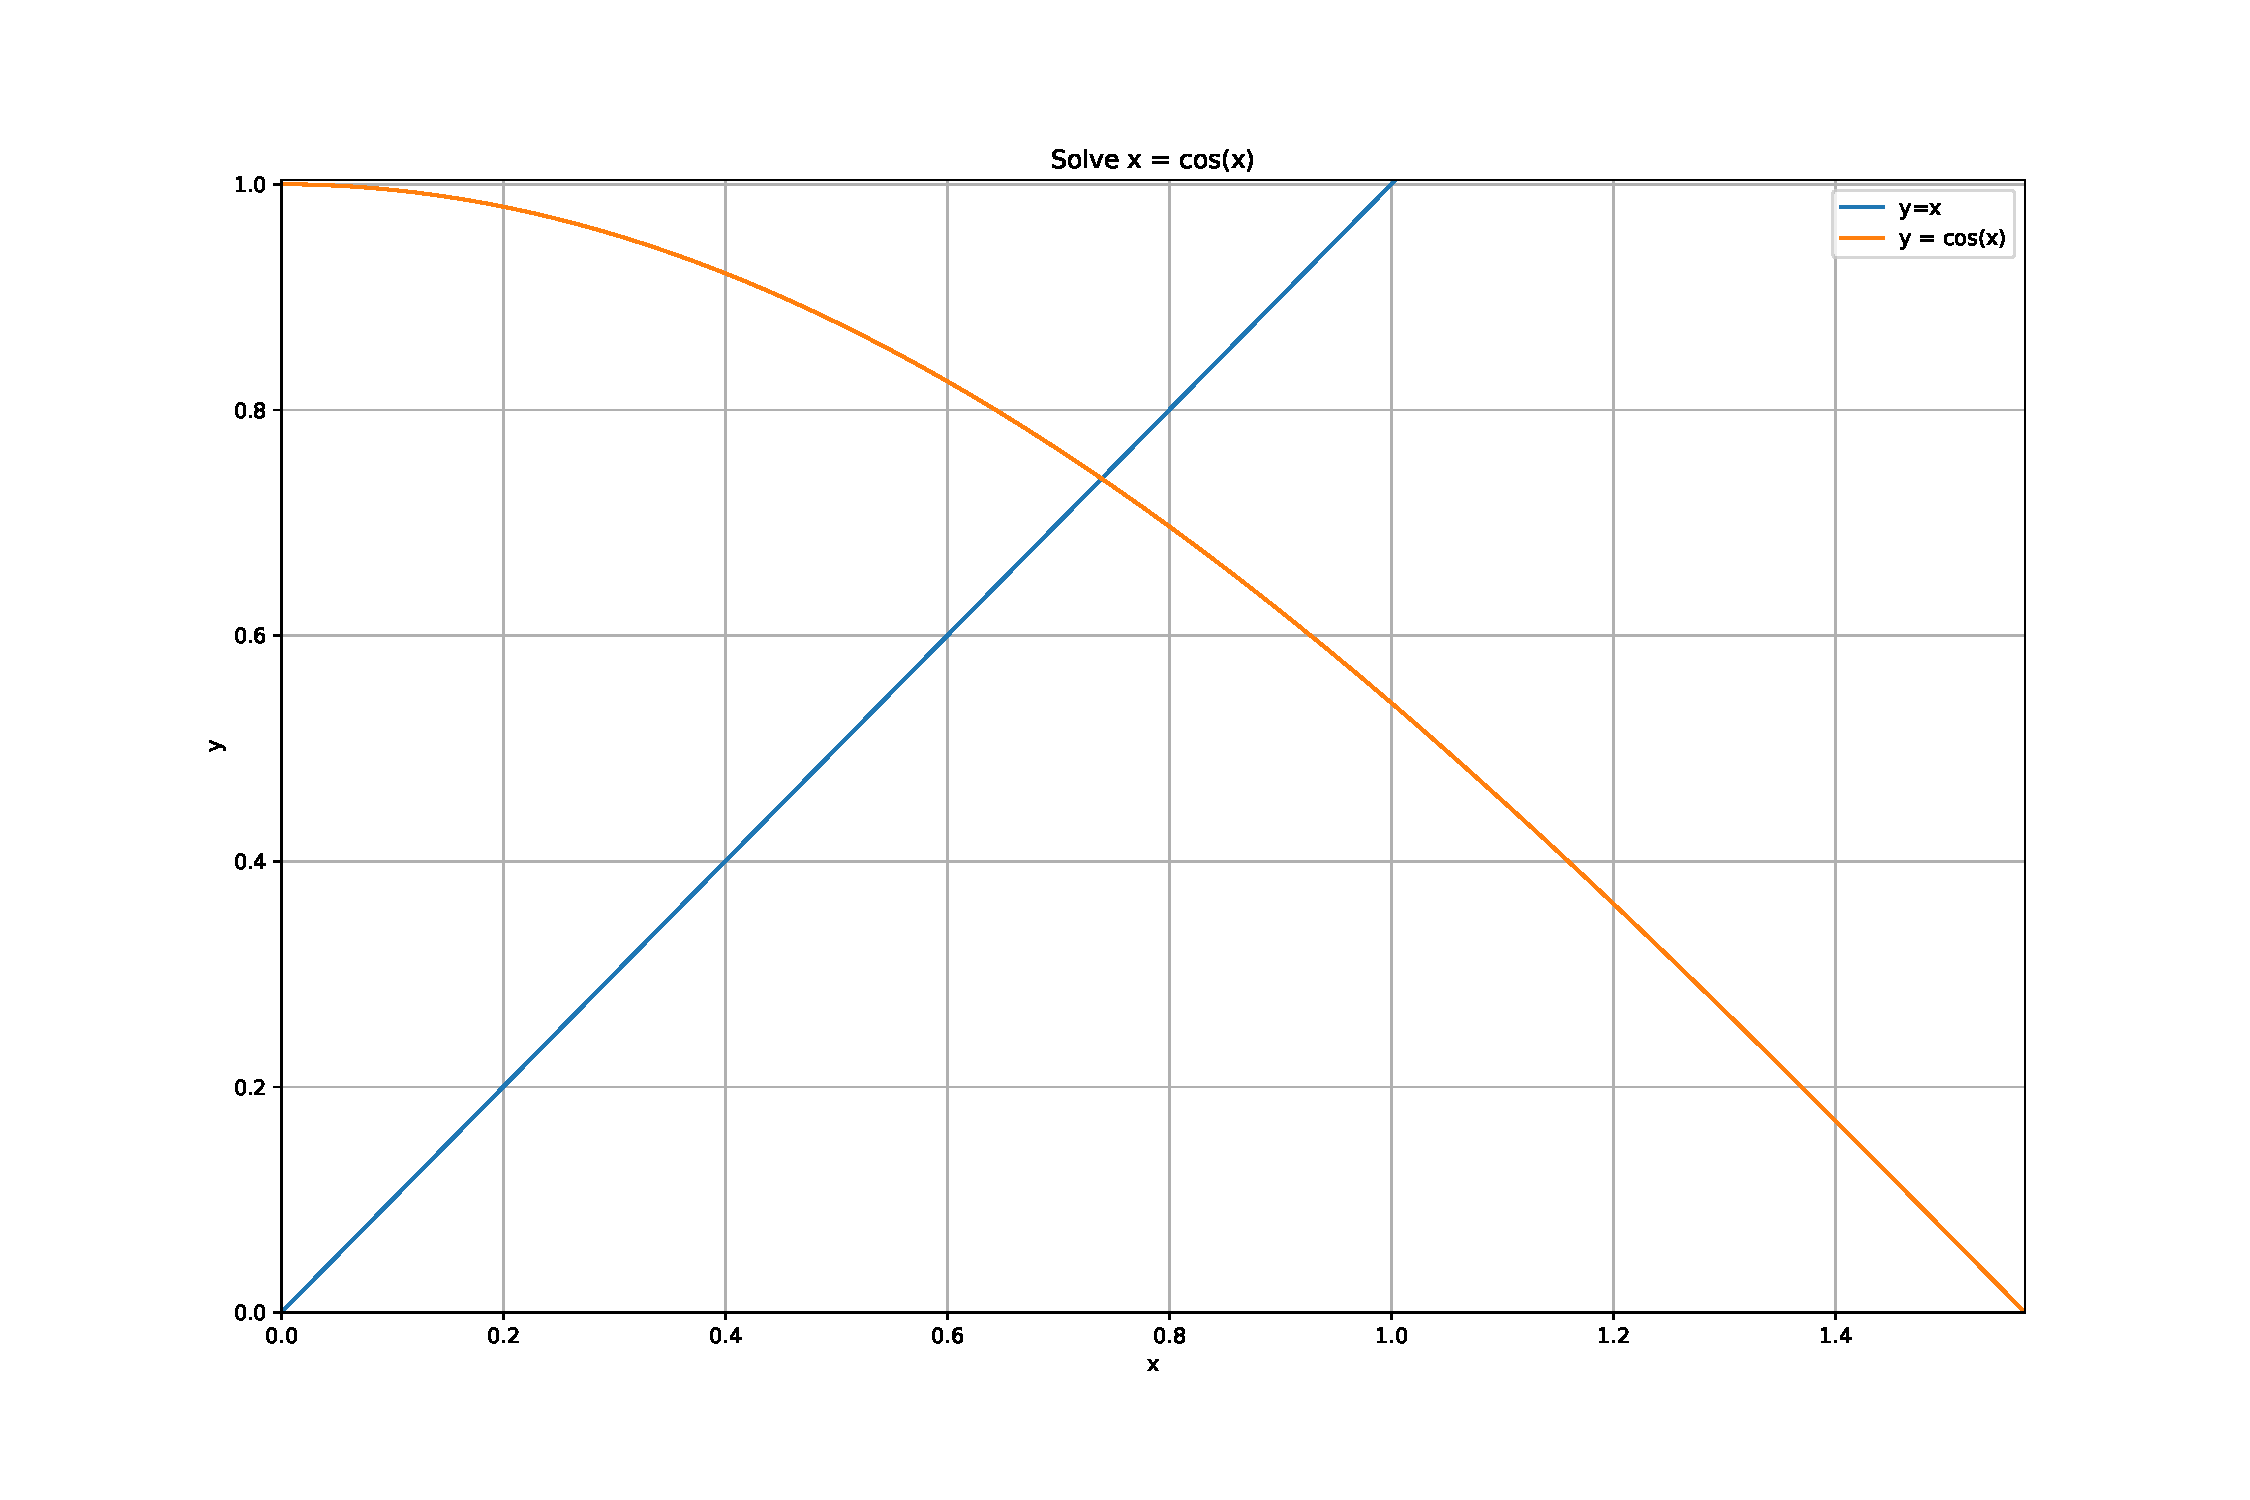
\epsfig{file=Figures/xEqualsCosX.pdf,scale=0.6}

  \caption{The functions $y = x$ and $y = cos(x)$.}
  \label{fig:xEqualsCosX.pdf}
\end{figure}



A simple approach that enables us to solve the equation $x = \cos(x)$ is to conduct a
\href{https://en.wikipedia.org/wiki/Fixed-point_iteration}{fixed-point iteration}.  To this end, we
define the sequence $\bigl(x_n\bigr)_{n\in\mathbb{N}}$ inductively as follows:
\\[0.2cm]
\hspace*{1.3cm} 
$x_0 = 0$ \quad and \quad $x_{n+1} = \mathtt{cos}(x_n)$ \quad for all $n \in \mathbb{N}$. 
\\[0.2cm]
With the help of the 
\href{https://en.wikipedia.org/wiki/Banach_fixed-point_theorem}{Banach fixed-point theorem}\footnote{
  The Banach fixed-point theorem is discussed in the lecture on
  \href{https://en.wikipedia.org/wiki/Differential_calculus}{differential calculus}.  This lecture is part of the
  second semester.
}
\index{Banach fixed-point theorem}
it can be shown that this sequence converges to a solution of the equation $x = \cos(x)$, i.e.~if we define
\\[0.2cm]
\hspace*{1.3cm}
$\bar{x} = \lim\limits_{n\rightarrow\infty} x_n$,
\\[0.2cm]
then we have
\\[0.2cm]
\hspace*{1.3cm}
$\cos\bigl(\bar{x}\bigr) = \bar{x}$.
\\[0.2cm]
Figure \ref{fig:solve.py} on page \pageref{fig:solve.py} shows the program
\href{https://github.com/karlstroetmann/Logic/blob/master/Python/solve.py}{\texttt{solve.py}}
that uses this approach to solve the equation $x = \cos(x)$.


\begin{figure}[!ht]
  \centering
\begin{minted}[ frame         = lines, 
                framesep      = 0.3cm, 
                numbers       = left,
                numbersep     = -0.2cm,
                bgcolor       = sepia,
                xleftmargin   = 0.8cm,
                xrightmargin  = 0.8cm,
              ]{python3}
    import math
    
    x     = 1.0
    old_x = 0.0
    i     = 1
    while abs(x - old_x) >= 4.0E-16:
        old_x = x
        x = math.cos(x)
        print(f'{i} : {x}')
        i += 1
\end{minted} 
\vspace*{-0.3cm}
\caption{Solving the equation $x = \cos(x)$ via fixed-point iteration.}  \label{fig:solve.py}
\end{figure} %\$

In this program, the iteration stops as soon as the difference between the variables \texttt{x} and 
\texttt{old\_x} is less that $4 \cdot 10^{-16}$.  Here, \texttt{x} corresponds to $x_{n+1}$, while \texttt{old\_x}
corresponds to $x_n$.  Once the values of $x_{n+1}$ and $x_n$ are sufficiently close, the execution of the \texttt{while} loop
terminates.
\href{https://github.com/karlstroetmann/Logic/blob/master/Python/Fixed-Point-Iteration.ipynb}{Fixed-Point-Iteration.ipynb}
shows a \textsl{Jupyter} notebook that implements fixed point iteration.


\begin{figure}[!ht]
\centering
\begin{minted}[ frame         = lines, 
                framesep      = 0.3cm, 
                firstnumber   = 1,
                numbers       = left,
                numbersep     = -0.2cm,
                bgcolor       = sepia,
                xleftmargin   = 0.8cm,
                xrightmargin  = 0.8cm,
              ]{python3}
    from math import cos
    
    def solve(f, x0):
        """
        Solve the equation f(x) = x using a fixed point iteration.
        x0 is the start value.
        """
        x = x0
        for n in range(10000):  # at most 10000 iterations
            oldX = x;
            x    = f(x);
            if abs(x - oldX) < 1.0e-15: 
                return x;
    
    print("solution to x = cos(x): ", solve(cos, 0));
    print("solution to x = 1/(1+x):", solve(lambda x: 1/(1+x), 0));
\end{minted}
\vspace*{-0.3cm}
\caption{A generic implementation of the fixed-point algorithm.}
\label{fig:fixpoint.py}
\end{figure}

Figure \ref{fig:fixpoint.py} on page \pageref{fig:fixpoint.py} shows the program
\href{https://github.com/karlstroetmann/Logic/blob/master/Python/fixpoint.py}{\texttt{fixpoint.py}}.
In this program we have implemented a function \texttt{solve} that takes two arguments.
\begin{enumerate}
\item \texttt{f} is a unary function.  The purpose of the \texttt{solve} is to compute the solution of the equation
      \\[0.2cm]
      \hspace*{1.3cm}
      $f(x) = x$.
      \\[0.2cm]
      This equation is solved with the help of a fixed-point algorithm.
\item \texttt{x0} is used as the initial value for the fixed-point iteration.
\end{enumerate}
Line 11 calls \texttt{solve} to compute the solution of the equation $x = \cos(x)$.
Line 12 solves the equation 
\\[0.2cm]
\hspace*{1.3cm}
$\ds x = \bruch{1}{1+x}$. 
\\[0.2cm]
This equation is equivalent to the quadratic equation $x^2 + x = 1$.  Note that we have defined the function
 $\ds x \mapsto \frac{1}{1+x}$ via the expression
 \\[0.2cm]
\hspace*{1.3cm}
\texttt{lambda x: 1/(1+x)}.
\\[0.2cm]
This expression is called an \blue{anonymous function} 
\index{lambda expression, \texttt{lambda x: f(x)}}
since we haven't given a name to the function.  

\remarkEng
The function \texttt{solve} is only able to solve the equation $f(x) = x$ if the function $f$ is a 
\href{https://en.wikipedia.org/wiki/Contraction_mapping}{contraction mapping} (Deutsch: \blue{kontrahierende Abbildung}). 
\index{contraction mapping}
  A function 
$f:\mathbb{R} \rightarrow \mathbb{R}$
is called a \blue{contraction mapping} iff 
\\[0.2cm]
\hspace*{1.3cm}
$|f(x) - f(y)| < |x - y|$ \quad for all $x,y \in \mathbb{R}$.
\\[0.2cm]
This notion will be discussed in more detail in the lecture on 
\href{https://github.com/karlstroetmann/Analysis/blob/master/Skript/analysis.pdf}{analysis} in the second
semester. \eox  

\section{Case Study: Computation of Poker Probabilities}
\index{poker}
In this short section we are going to show how to compute probabilities for the
\href{https://en.wikipedia.org/wiki/Texas_hold_%27em}{\textsl{Texas Hold'em}} variation of 
\href{https://en.wikipedia.org/wiki/Poker}{poker}.   Texas Hold'em poker is played with a deck of 52
cards.  Every card has a \blue{value}.  This value is an element of the set
\\[0.2cm]
\hspace*{1.3cm} 
$\textsl{Values} = \{ 2, 3, 4, 5, 6, 7, 8, 9, 10, \textsl{Jack}, \textsl{Queen}, \textsl{King}, \textsl{Ace} \}$.
\\[0.2cm]
Furthermore, every card has a \blue{suit}.  This suit is an element of the set
\\[0.2cm]
\hspace*{1.3cm} 
$\textsl{Suits} = \{ \club, \mbox{$\color{red}{\heart}$}, \mbox{$\color{red}{\diamondsuit}$}, \spade \}$.
\\[0.2cm]
These suits are pronounced \blue{club}, \blue{heart}, \blue{diamond}, and \blue{spade}.
As a card is determined by its value and its suit, a card can be represented as a pair $\pair(v,s)$, where $v$
denotes the value while $s$ is the suit of the card.  Hence, the set of all cards can be represented as the set
\\[0.2cm]
\hspace*{1.3cm} 
$\textsl{Deck} = \bigl\{ \pair(v,s) \mid v \in \textsl{Values} \wedge \textsl{s} \in \textsl{Suits} \bigr\}$.
\\[0.2cm]
At the start of a game of Texas Hold'em, every player receives two cards.  These two cards are known
as the \blue{preflop} or the \blue{hole}.  Next, there is a \blue{bidding phase} where players can bet on their
cards.   After this bidding phase, the dealer puts three cards open on the table.  These three cards are
known as \blue{flop}.  Let us assume that a player has been dealt the set of cards
\\[0.2cm]
\hspace*{1.3cm}
$\{ \pair(3, \club), \pair(3, \spade) \}$.
\\[0.2cm]
This set of cards is known as a \blue{pocket pair}.  Then the player would like to know the probability
that the flop will contain another card with value $3$, as this would greatly increase her chance of
winning the game.  In order to compute this probability we have to compute the number of possible
flops that contain a card with the value $3$ and we have to divide this number by the number of all
possible flops:
\\[0.2cm]
\hspace*{1.3cm}
$\ds \frac{\;\mbox{number of flops containing a card with value $3$}\;}{\mbox{number of all possible flops}}$
\\[0.2cm]
The program
\href{https://github.com/karlstroetmann/Logic/blob/master/Python/poker-triple.py}{poker-triple.py}
shown in Figure \ref{fig:poker-triple.py} performs this computation.  We proceed to discuss this
program line by line.


\begin{figure}[!ht]
\centering
\begin{minted}[ frame         = lines, 
                framesep      = 0.3cm, 
                numbers       = left,
                numbersep     = -0.2cm,
                bgcolor       = sepia,
                xleftmargin   = 0.0cm,
                xrightmargin  = 0.0cm,
              ]{python3}
    Values = { "2", "3", "4", "5", "6", "7", "8", "9", "T", "J", "Q", "K", "A" } 
    Suits  = { "c", "h", "d", "s" }
    Deck   = { (v, s) for v in Values for s in Suits }
    Hole   = { ("3", "c"), ("3", "s") }
    Rest   = Deck - Hole
    Flops  = { (k1, k2, k3) for k1 in Rest for k2 in Rest for k3 in Rest 
                            if  len({ k1, k2, k3 }) == 3 
             }
    Trips  = { f for f in Flops if ("3", "d") in f or ("3", "h") in f }
    print(len(Trips) / len(Flops))
\end{minted}
\vspace*{-0.3cm}
\caption{Computing a probability in poker.}
\label{fig:poker-triple.py}
\end{figure}

\begin{enumerate}
\item In line 1 the set \texttt{Values} is defined to be the set of all possible values that a card
      can take.  In defining this set we have made use of the following abbreviations:
      \begin{enumerate}
      \item ``\texttt{T}'' is short for ``\blue{Ten}'',
      \item ``\texttt{J}'' is short for ``\blue{Jack}'',
      \item ``\texttt{Q}'' is short for ``\blue{Queen}'',
      \item ``\texttt{K}'' is short for ``\blue{King}'', and
      \item ``\texttt{A}'' is short for ``\blue{Ace}''.
      \end{enumerate}
\item In line 2 the set \texttt{Suits} represents the possible suits of a card.  Here, we have used
      the following abbreviations:
      \begin{enumerate}
      \item ``\texttt{c}'' is short for $\club$ (\underline{c}lub), 
      \item ``\texttt{h}'' is short for \mbox{\color{red}{$\heart$}} (\underline{h}earts), 
      \item ``\texttt{d}'' is short for \mbox{\color{red}{$\diamondsuit$}} (\underline{d}iamonds), and 
      \item ``\texttt{s}'' is short for $\spade$ (\underline{s}pades). 
      \end{enumerate} 
\item Line 3 defines the set of all cards.  This set is stored as the variable \texttt{Deck}.  Every
      card is represented as a pair of the form $(v,s)$. Here, $v$ is the value of the card, while $s$ is its suit.
\item Line 4 defines the set \texttt{Hole}.  This set represents the two cards that have been given to our player.
\item The remaining cards are defined as the variable  \texttt{Rest} in line 5.
\item Line 6 computes the set of all possible flops.  Since the order of the cards in the flop does
      not matter, we use sets to represent these flops.  However, we have to take care that the flop
      does contain three \colorbox{amethyst}{different} cards.  Hence, we have to ensure that the three
      cards \texttt{k1}, \texttt{k2}, and \texttt{k3} that make up the flop satisfy the inequalities 
      \\[0.2cm]
      \hspace*{1.3cm}
      $\mathtt{k1} \not= \mathtt{k2}$, \quad $\mathtt{k1} \not= \mathtt{k3}$,  \quad and \quad $\mathtt{k2} \not= \mathtt{k3}$.
      \\[0.2cm]
      These inequalities are satisfied if and only if the set 
      $\{ \mathtt{k1}, \mathtt{k2}, \mathtt{k3} \}$ contains exactly three elements.  Hence, when
      choosing \texttt{k1}, \texttt{k2}, and \texttt{k3} we have to make sure that the condition
      \\[0.2cm]
      \hspace*{1.3cm}
      $\texttt{len}\bigl({\{ \mathtt{k1}, \mathtt{k2}, \mathtt{k3} \} \;\mathtt{==}\; 3 }\bigr)$
      \\[0.2cm]
      holds.
\item Line 9 computes the subset \texttt{Trips} of those flops that contain at least one card with a value of 3.
      As the 3 of clubs and the 3 of spades have already been dealt to our player, the only cards
      with value 3 that are left in the deck are the 3 of diamonds and the 3 of hearts.  Therefore, we are looking for
      those flops that contain one of these two cards.
\item Finally, the probability for obtaining another card with a value of 3 in the flop is computed as
      the ratio of the number of flops containing a card with a value of 3 to the number of all possible flops.
\end{enumerate}
When we run the program we see that the probability of improving a \blue{pocket pair} on the flop to \blue{trips} or better
is about  $11.8\%$.  A \textsl{Jupyter} notebook showcasing this computation outlined above can be fount at
\href{https://github.com/karlstroetmann/Logic/blob/master/Python/Poker.ipynb}{Poker.ipynb}.

\remarkEng
The method to compute probabilities that has been sketched above only works if the sets that have to
be computed are small enough to be retained in memory.  If this condition is
not satisfied we can use the \href{https://en.wikipedia.org/wiki/Monte_Carlo_method}{\emph{Monte Carlo method}} 
\index{Monte Carlo method} 
to compute the probabilities instead.  This method will be discussed in the lecture on 
\href{https://github.com/karlstroetmann/Algorithms/blob/master/Lecture-Notes/algorithms.pdf}{algorithms}.


\section{Finding a Path in a Graph}
In the following section, I will present an application that is more interesting since it is practically
relevant.  In order to prepare for this, we will now discuss the problem of finding a \blue{path} \index{path}
in a
\href{https://en.wikipedia.org/wiki/Directed_graph}{directed graph}. 
\index{directed graph}
Abstractly, a \emph{directed graph} consists of \blue{vertices} and \blue{edges} that connect these vertices.  In an application, the
vertices could be towns and villages, while the edges would be interpreted as one-way streets connecting these
villages.  To simplify matters, let us assume for now that the vertices are given as natural numbers.  As the
edges represent connections between vertices,  the edges are represented as pairs of natural numbers.  Then,
the graph can be represented as the set of its edges, as the set of vertices is implicitly given once the edges
are known.  To make things concrete, let us consider an example.  In this case, the set of edges is called
\texttt{R} and is defined as follows:  
\\[0.2cm]
\hspace*{1.3cm}
$\texttt{R}\; \mathtt{=}\; \bigl\{ \pair(1,2), \pair(2,3), \pair(1,3), \pair(2,4), \pair(4,5) \bigr\}$.
\\[0.2cm]
In this graph, the set of vertices is given as
\\[0.2cm]
\hspace*{1.3cm}
$\{ 1, 2, 3, 4, 5 \}$.
\\[0.2cm]
This graph is shown in Figure \ref{fig:graph0} on page \pageref{fig:graph0}.  You should note that the
connections between vertices that are given in this graph are \blue{unidirectional}:  While there is a connection from
vertex $1$ to vertex $2$, there is no connection from vertex $2$ to vertex $1$.

 
\begin{figure}[!ht]
  \centering
  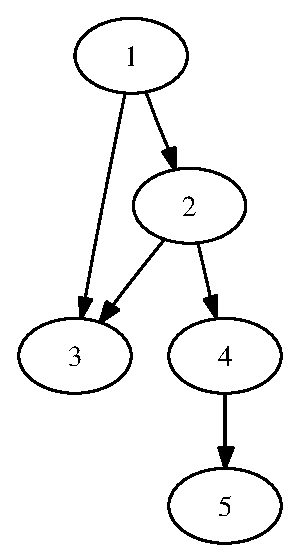
\epsfig{file=Figures/graph0,scale=0.6}

  \caption{A simple graph.}
  \label{fig:graph0}
\end{figure}



\noindent
The graph given by the relation \texttt{R} contains only the direct connections of vertices.  For example, in
the graph shown in Figure \ref{fig:graph0}, there is a direct connection from vertex $1$ to vertex $2$ and
another direct connection from vertex $2$ to vertex $4$.  Intuitively, vertex $4$ is reachable from vertex $1$,
since from vertex $1$ we can first reach vertex $2$ and from vertex $2$ we can then reach vertex $4$.  However,
there is is no direct connection between the vertices $1$ and $4$.  To make this more formal, define
a \blue{path} of a graph $R$ as a list of vertices
\\[0.2cm]
\hspace*{1.3cm}
$[x_1, x_2, \cdots, x_n]$ \quad such that \quad $\pair(x_i,x_{i+1}) \in R$ \quad for all $i=1,\cdots,n-1$.
\\[0.2cm]
In this case, the path $[x_1, x_2, \cdots, x_n]$ is written as
\\[0.2cm]
\hspace*{1.3cm}
$x_1 \mapsto x_2 \mapsto \cdots \mapsto x_n$
\\[0.2cm]
and has the \blue{length} $n-1$, since there are $n-1$ direct connections of the form $\pair(x_i,x_{i+1})$ that
make up this path.
To put it differently,  the length of a path
$[x_1,x_2,\cdots,x_n]$ is defined as the number of edges connecting the vertices and not as the
number of vertices appearing on the path.

Furthermore,  two vertices $a$ and $b$ of a graph are said to be \blue{connected} \index{connected} iff there exists a path
\\[0.2cm]
\hspace*{1.3cm}
$[x_1,\cdots,x_n]$ \quad such that \quad $a = x_1$ \quad and \quad $b = x_n$.
\\[0.2cm]
The goal of this section is to develop an algorithm that checks whether two vertices $a$ and $b$ are connected.
Furthermore, we want to be able to compute the corresponding path connecting the vertices $a$ and $b$.


\subsection{Computing the Transitive Closure of a Relation}
We have already noted that a graph can be represented as the set of its edges and hence as a \blue{binary relation}.
We have previously defined a \blue{binary relation} as a set of pairs.  We also need the notion of a
\blue{relational product}: \index{relational product, $Q \circ R$}
If $Q$ and $R$ are binary relations, then the \blue{relational product} $Q \circ R$ of $Q$ and $R$ is defined as
\\[0.2cm]
\hspace*{1.3cm}
$Q \circ R := \Bigl\{ \pair(x, z) \Bigm| \exists y:\bigl(\pair(x,y) \in Q \wedge \pair(y,z) \in R\bigr) \Bigr\}$.
\\[0.2cm]
Furthermore, for any $n \in \mathbb{N}^*$ we can define the $n$-th power $R^n$ of the relation $R$ by induction.
\begin{description}
\item[Base Case:] $n = 1$.

             $R^1 := R$
\item[Induction Step:] $n \mapsto n+1$ 

             $R^{n+1} := R^n \circ R$.
\end{description}
The idea behind this definition is that if $\pair(x, z) \in R^n$, then there is a path of length $n$ that
starts in $x$ and ends in $z$.

In order to decide whether there is a path connecting two vertices we have to compute the 
\href{https://en.wikipedia.org/wiki/Transitive_closure}{transitive closure} $R^+$ of a relation $R$.  
To understand this notion, we first need to define the concept of \blue{transitivity}:  A relation $R$ is
transitive if and only if the following holds:
\\[0.2cm]
\hspace*{1.3cm}
$\pair(x,y) \in T \wedge \pair(y, z) \in T \rightarrow \pair(x, z) \in T$ \quad for all $x,y,z$. 
\\[0.2cm]
Now the \blue{transitive closure} $R^+$ 
\index{transitive closure $R^+$}
of a binary relation $R$ is the \blue{smallest} relation $T$ such that the following
conditions hold:
\begin{itemize}
\item $R$ is a subset of $T$, i.e. we have $R \subseteq T$.
\item $T$ is transitive.
\end{itemize}
The lecture on
\href{https://github.com/karlstroetmann/Lineare-Algebra/blob/master/Skript/lineare-algebra.pdf}{Lineare Algebra} 
gives a prove that the transitive closure $R^+$ of a binary relation can be computed as follows:
\\[0.2cm]
\hspace*{1.3cm}
$R^+ = \bigcup\limits_{n=1}^{\infty} R^n = R^1 \cup R^2 \cup R^3 \cup \cdots$  
\\[0.2cm]
Initially, this formula might look intimidating as it suggests an infinite computation.
Fortunately, it turns out that we do not have to compute the powers $R^n$ for every $n \in \mathbb{N}$.  Let me
explain the reason that allows us to cut the computation short.  
\begin{enumerate}
\item $R$ is the set of direct connections between two vertices.
\item $R^2$ is the same as $R \circ R$ and this relational product is defined as
      \\[0.2cm]
      \hspace*{1.3cm}
       $R \circ R = \bigl\{ \pair(x,z) \bigm| \exists y \colon(\pair(x,y) \in R \wedge \pair(y,z)) \in R \bigr\}$.
      \\[0.2cm]
      Hence, $R \circ R$ contains those pairs $\pair(x,z)$ that are connected via one intermediate vertex $y$,
      i.e.~there is a path of the form $x \mapsto y \mapsto z$ that connects $x$ and $z$.  This path
      has length 2.  In general, we can show by induction on $n$ that $R^n$ connect those pairs that are
      connected by a path of length $n$.  The induction step of this proof runs as follows:

      $R^{n+1}$ is defined as $R^n \circ R$ and therefore we have
      \\[0.2cm]
      \hspace*{1.3cm}
      $R^n \circ R = \{ \pair(x,z) \mid \exists y \colon \pair(x,y) \in R^n \wedge \pair(y,z) \in R \}$.
      \\[0.2cm]
      As $\pair(x,y) \in R^n$, the induction hypothesis guarantees that the vertices $x$ and $y$ are
      connected by a path of length $n$.  Hence, this 
      path has the form
      \\[0.2cm]
      \hspace*{1.3cm}
      $\underbrace{x \mapsto \cdots \mapsto y}_{\mbox{\scriptsize path of length $n$.}}$
      \\[0.2cm]
      Adding $z$ at the end of this path will produce the path
      \\[0.2cm]
      \hspace*{1.3cm}
      $\underbrace{\underbrace{x \mapsto \cdots \mapsto y}_{\mbox{\scriptsize path of length $n$.}} \mapsto z}_{\mbox{\scriptsize path of length $n+1$.}}$.
      \\[0.2cm]
      This path has a length of $n + 1$ and, furthermore, connects $x$ and $z$.  Hence $R^{n+1}$
      contains those pairs $\pair(x, z)$ that are connected by a path of length $n+1$.
\end{enumerate}
Now the important observation is the following. The set of all vertices is finite.  For the arguments sake, let
us assume there are $k$ different vertices.  But then every path that has a length of $k$ or greater must
contain at least one vertex that is visited more than once and hence this path is longer than necessary,
i.e.~there is a shorter path that connects the same vertices.  Therefore, for a finite graph with $k$ vertices,
the formula to compute the transitive closure can be simplified as follows:
\\[0.2cm]
\hspace*{1.3cm} 
$\ds R^+ = \bigcup\limits_{i=1}^{k-1} R^i$.
\\[0.2cm]
While we could use this formula as its stands, it is more efficient to use a \blue{fixed-point iteration} instead.
To this end, we prove that the transitive closure $R^+$ satisfies the following equation:
\begin{equation}
  \label{fixpunkt}
  R^+ = R \cup R^+ \circ R. 
\end{equation}
The precedence of the operator $\circ$ 
is higher than the precedence of the operator $\cup$.  Therefore, the expression $R \cup R^+ \circ R$ is
equivalent to the expression $R \cup (R^+ \circ R)$.  In order to prove equation \ref{fixpunkt} we first note
that the following  \blue{law of distributivity} holds:
\\[0.2cm]
\hspace*{1.3cm}
$\ds (P \cup Q) \circ R = (P \circ R) \cup (Q \circ R)$.
\\[0.2cm]
(A proof of this equation can be found in my lecture notes on
\href{https://github.com/karlstroetmann/Lineare-Algebra/blob/master/Skript/lineare-algebra.pdf}{linear algebra}
on page 42.)  Using this law, we can prove equation \ref{fixpunkt} algebraically.  We have:
\\[0.2cm]
\hspace*{1.3cm}
$
\begin{array}{cll}
    & R \cup R^+ \circ R \\[0.2cm]
  = & R \cup \Bigl(\bigcup\limits_{i=1}^{\infty} R^i \Bigr) \circ R \\[0.4cm]
  = & R \cup \bigl(R^1 \cup R^2 \cup R^3 \cup \cdots \bigr) \circ R \\[0.2cm]
  = & R \cup \bigl(R^1 \circ R \cup R^2 \circ R \cup R^3 \circ R \cup \cdots \bigr) \\[0.2cm]
  = & R \cup \bigl(R^2 \cup R^3 \cup  R^4 \cup \cdots \bigr)  \\[0.2cm]
  = & R^1 \cup R^2 \cup R^3 \cup  R^4 \cup \cdots  \\[0.2cm]
  = & \bigcup\limits_{i=1}^{\infty} R^i \\[0.4cm]
  = & R^+.
\end{array}
$
\\[0.2cm]
Equation  \ref{fixpunkt} can now be used to compute $R^+$ via a fixed-point iteration.
To this end, let us define a sequence of relations $(T_n)_{n \in \mathbb{N}}$ by induction on $n$:
\begin{enumerate}
\item[I.A.] $n = 0$: 

            $T_0 = R$
\item[I.S.] $n \mapsto n+1$:

            $T_{n+1} = R \cup T_n \circ R $. 
\end{enumerate}
The relation  $T_n$ can be expressed via the relation $R$, we have
\begin{enumerate}
\item $T_0 = R$.
\item $T_1 = R \cup T_0 \circ R = R \cup R \circ R = R^1 \cup R^2$.
\item$\begin{array}[t]{lcl}
       T_2  & = & R \cup T_1 \circ R \\
            & = & R \cup (R^1 \cup R^2) \circ R \\
            & = & R^1 \cup R^2 \cup R^3. \\
       \end{array}
      $
\end{enumerate}
In general, we can show by induction that
\\[0.2cm]
\hspace*{1.3cm}
$\ds T_n = \bigcup\limits_{i=1}^{n+1} R^i$
\\[0.2cm]
holds for all $n \in \mathbb{N}$.  As $R^1 = R$, the base case $n=0$ of this proof is immediate from the definition of $T_0$.
In the induction step we observe the following:
\\[0.2cm]
\hspace*{1.3cm}
$
 \begin{array}{lcll}
   T_{n+1} & = & \ds R \cup T_n \circ R & \mbox{(by definition)} \\[0.2cm]
           & = & \ds R \cup \biggl(\bigcup\limits_{i=1}^{n+1} R^i\biggr) \circ R &
                 \mbox{(by induction hypothesis)} \\[0.4cm]
           & = & \ds R \cup \left(R \cup \cdots \cup R^{n+1}\right) \circ R \\[0.2cm] 
           & = & \ds R^1 \cup R^2 \cup \cdots \cup R^{n+2}  &
                 \mbox{(by the distributivity of $\circ$ over $\cup$)} \\[0.2cm]
           & = & \ds \bigcup\limits_{i=1}^{n+2} R^i & \Box 
   \end{array}
$
\\[0.2cm]
The sequence $(T_n)_{n\in\mathbb{N}}$ has another useful property:  It is 
\blue{monotonically increasing}.  In general, a sequence of sets $(X_n)_{n\in\mathbb{N}}$ is called
\blue{monotonically increasing} iff we have \index{monotonically increasing}
\\[0.2cm]
\hspace*{1.3cm}
$\forall n \in \mathbb{N}: X_n \subseteq X_{n+1}$,
\\[0.2cm]
i.e.~the sets $X_n$ get bigger with growing index $n$.
The monotonicity of the sequence  $(T_n)_{n \in \mathbb{N}}$ is an immediate consequence of the equation
\\[0.2cm]
\hspace*{1.3cm}
$\ds T_n = \bigcup\limits_{i=1}^{n+1} R^i$ 
\\[0.2cm]
because we have:
\\[0.2cm]
\hspace*{1.3cm}
$
\begin{array}[t]{llcl}
                & \ds T_n \subseteq T_{n+1} \\[0.2cm]
\Leftrightarrow & \ds \bigcup\limits_{i=1}^{n+1} R^i \subseteq \bigcup\limits_{i=1}^{n+2} R^i \\[0.5cm]
\Leftrightarrow & \ds \bigcup\limits_{i=1}^{n+1} R^i \subseteq \left(\bigcup\limits_{i=1}^{n+1} R^i\right) \cup R^{n+2} \\
\end{array}
$
\\[0.2cm]
If the relation  $R$ is finite, then the transitive closure $R^+$ is finite, too.  All of the sets $T_n$ 
are subsets of $R^+$ because we have
\\[0.2cm]
\hspace*{1.3cm}
$\ds T_n = \bigcup\limits_{i=1}^{n+1} R^i \subseteq \bigcup\limits_{i=1}^{\infty} R^i = R^+$ \quad for all $n \in \mathbb{N}$.
\\[0.2cm]
Hence the sets $T_n$ can not grow indefinitely.  Because of the monotonicity of the sequence 
$(T_n)_{n\in\mathbb{N}}$ it follows that there exists an index  $k \in \mathbb{N}$ such that the sets $T_n$ do
not grow any further once $n$ has reached $k$, i.e.~we have
\\[0.2cm]
\hspace*{1.3cm}
$\ds \forall n \in \mathbb{N}:( n \geq k \rightarrow T_n = T_k)$.
\\[0.2cm]
But this implies that
\\[0.2cm]
\hspace*{1.3cm}
$\ds T_n = \bigcup\limits_{i=1}^{n+1} R^i = \bigcup\limits_{i=1}^{\infty} R^i = R^+$ 
\quad holds for all $n \geq k$.
\\[0.2cm]
Therefore, the algorithm for computing  $R^+$ iterates the equation 
\\[0.2cm]
\hspace*{1.3cm}
$\ds T_{n+1} = R \cup T_n \circ R$
\\[0.2cm]
until the equation  $T_{n+1} = T_n$ is satisfied, since this implies that $T_n = R^+$.


\begin{figure}[!ht]
  \centering
\begin{minted}[ frame         = lines, 
                framesep      = 0.3cm, 
                numbers       = left,
                numbersep     = -0.2cm,
                bgcolor       = sepia,
                xleftmargin   = 0.8cm,
                xrightmargin  = 0.8cm,
              ]{python3}
    def product(R1, R2):
        'Compute the relational product of R1 and R2.'
        return { (x, z) for (x, y1) in R1 for (y2, z) in R2 if y1 == y2 }
    
    def transClosure(R):
        'Compute the transitive closure of the binary relation R.'
        T = R
        while True:
            oldT = T
            T    = product(R,T) | R
            if T == oldT:
                return T
    
    R = { (1,2), (2,3), (1,3), (2,4), (4,5) }
    print( 'R  = ', R );
    print( 'Computing the transitive closure of R:' );
    T = transClosure(R);
    print( 'R+ = ', T );
\end{minted} 
\vspace*{-0.3cm}
\caption{Computing the transitive closure.}  
\label{fig:transitive-closure.py}
\end{figure} %\$

\noindent
The program 
\href{https://github.com/karlstroetmann/Logic/blob/master/Python/transitive-closure.py}{\texttt{transitive-closure.py}}
that is shown in Figure
\ref{fig:transitive-closure.py} on page \pageref{fig:transitive-closure.py} shows an implementation of this idea.
The program produces the following output:
\begin{verbatim}
    R  = {(1, 2), (1, 3), (4, 5), (2, 3), (2, 4)}
    Computing the transitive closure of R:
    R+ = {(1, 2), (1, 3), (4, 5), (1, 4), (1, 5), (2, 3), (2, 5), (2, 4)}
\end{verbatim}
The transitive closure $R^+$ of a relation $R$ has a very intuitive interpretation:
It contains all pairs $\pair(x,y)$ such that there is a path leading from 
$x$ to $y$.  
The function $\texttt{product}(R_1, R_2)$ computes the relational product $R_1\circ R_2$ 
according to the formula
\\[0.2cm]
\hspace*{1.3cm}
$R_1 \circ R_2 = \Bigl\{ \langle x, z \rangle \Bigm| \exists y:\bigl(\pair(x,y) \in R_1 \wedge \pair(y,z) \in R_2\bigr) \Bigr\}$.


\subsection{Computing the Paths}
So far, given a graph represented by a relation $R$ and two vertices $x$ and $y$, we can only check
whether there is a path leading from $x$ to $y$, but we cannot compute this path.  In this
subsection we will extend the procedure \texttt{transClosure} so that it will also compute the
corresponding path.  The main idea is to extend the notion of a relational product to the notion of
a \blue{path product}, where a \blue{path product} is defined on sets of paths.  In order to do so,
we introduce three functions for tuples.
\begin{enumerate}
\item Given a tuple $T$, the function $\texttt{first}(T)$ returns the first element of $T$: 
      \\[0.2cm]
      \hspace*{1.3cm}
      $\texttt{first}\bigl(\langle x_1,\cdots,x_m\rangle\bigr) = x_1$.
\item Given a tuple $T$, the function $\texttt{last}(T)$ returns the last element of $T$: 
      \\[0.2cm]
      \hspace*{1.3cm}
      $\texttt{last}\bigl(\langle x_1,\cdots,x_m\rangle\bigl) = x_m$.
\item If $S = \langle x_1, \cdots, x_m\rangle$ and $T = \langle y_1, \cdots, y_n \rangle$ are two tuples  such that
      $\texttt{first}(T) = \texttt{last}(S)$, we define the \blue{join} $S \oplus T$ of $S$ and $T$ as \\[0.2cm]
      \hspace*{1.3cm}
      $S \oplus T = \langle x_1, \cdots, x_m, y_2, \cdots, y_n \rangle$.
\end{enumerate}
If $\mathcal{P}_1$ and $\mathcal{P}_2$ are sets of tuples representing paths, we define the \blue{path product} of
$\mathcal{P}_1$ and $\mathcal{P}_2$ as follows: \\[0.2cm]
\hspace*{1.3cm} 
$\mathcal{P}_1 \bullet \mathcal{P}_2 = 
\bigl\{\; T_1 \oplus T_2 \mid T_1 \in \mathcal{P}_1 \wedge T_2 \in \mathcal{P}_2 \wedge \texttt{last}(T_1) = \texttt{first}(T_2) \;\bigr\}
$.

\begin{figure}[!ht]
  \centering
\begin{minted}[ frame         = lines, 
                framesep      = 0.3cm, 
                numbers       = left,
                numbersep     = -0.2cm,
                bgcolor       = sepia,
                xleftmargin   = 0.8cm,
                xrightmargin  = 0.8cm,
              ]{python3}
    def findPaths(R):
        P = R;
        while True:
            oldP = P
            P    = R | pathProduct(P, R)
            if P == oldP:
                return P

    def pathProduct(P, Q):
        return { join(S, T) for S in P for T in Q if S[-1] == T[0] }
    
    def join(S, T):
        return S + T[1:]
    
    R = { (1,2), (2,3), (1,3), (2,4), (4,5) }
    print('R = ', R)
    print('Computing all paths:' )
    P = findPaths(R)
    print('P = ', P)
\end{minted} 
\vspace*{-0.3cm}
\caption{Computing all connections.}  \label{fig:path.py}
\end{figure} %\$

\begin{figure}[!ht]
  \centering
  \vspace*{-9cm}

  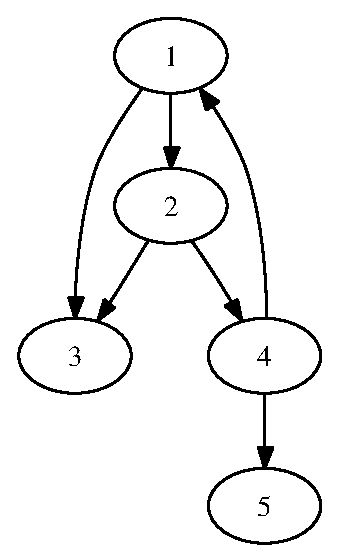
\epsfig{file=Figures/graph-zykl,scale=0.5}
  \vspace*{-1cm}

  \caption{A graph with a cycle.}
  \label{fig:graph-zykl}
\end{figure}

Using the notion of a \blue{path product} we are able to extend the program shown in Figure
\ref{fig:transitive-closure.py} such that it computes all paths between two vertices.
The resulting program
\href{https://github.com/karlstroetmann/Logic/blob/master/Python/path.py}{\texttt{path.py}}
is shown in Figure \ref{fig:path.py} on page \pageref{fig:path.py}.
Unfortunately, the program does not work any more if the graph is \blue{cyclic}.  A graph is defined
to be \blue{cyclic} if there is a path of length greater than $1$ that starts and ends at the same
vertex.  This path is then called a \blue{cycle}.
Figure \ref{fig:graph-zykl} on page \pageref{fig:graph-zykl} shows a cyclic graph.  This graph is
cyclic because it contains the path
\\[0.2cm]
\hspace*{1.3cm}
$\langle 1, 2, 4, 1 \rangle$
\\[0.2cm]
and this path is a cycle.
The problem with this graph is that it contains an infinite number of paths that connect the vertex
1 with the vertex 2: \\[0.2cm]
\hspace*{1.3cm}
$\langle 1, 2 \rangle$, $\langle 1, 2, 4, 1, 2 \rangle$, 
$\langle 1, 2, 4, 1, 2, 4, 1, 2 \rangle$, 
$\langle 1, 2, 4, 1, 2, 4, 1, 2, 4, 1, 2 \rangle$, $\cdots$
\\[0.2cm]
Of course, there is no point in computing a path that visits a vertex more than once as these paths
contain cycles.  Our goal is to eliminate all those paths that contain cycles.


\begin{figure}[!ht]
  \centering
\begin{minted}[ numbers       = left,
                numbersep     = -0.2cm,
                frame         = lines, 
                framesep      = 0.3cm, 
                bgcolor       = sepia,
                xleftmargin   = 0.0cm,
                xrightmargin  = 0.0cm,
             ]{python3}
    def pathProduct(P, Q):
        return { join(S, T) for S in P for T in Q
                            if S[-1] == T[0] and noCycle(S, T)
               }
    
    def noCycle(T1, T2):
        return len({ x for x in T1 } & { x for x in T2 }) == 1
\end{minted} 
\vspace*{-0.3cm}
\caption{Computing the connections in a cyclic graph.}  
\label{fig:path-cyclic.py}
\end{figure} %\$

Figure \ref{fig:path-cyclic.py} on page shows how the implementation of the function
\texttt{pathProduct} has to be changed so that the resulting program
\href{https://github.com/karlstroetmann/Logic/blob/master/Python/path-cyclic.py}{\texttt{path-cyclic.py}}
works also for cyclic graphs. 
\begin{enumerate}
\item In line 2 and 3, we compute only those paths that are not cyclic.
\item Line 6 defines a function \texttt{noCycle} that tests, whether the join  $\texttt{T1} \oplus \texttt{T2}$ is cyclic.  The join
      of \texttt{T1} and \texttt{T2} is cyclic iff the tuples \texttt{T1} and \texttt{T2} have more
      than one common element.  The tuples \texttt{T1} and \texttt{T2} will always have at least one common element, as we join
      these tuples only if the last element of \texttt{T1} is equal to the first element of  \texttt{T2}.
      If there would be an another vertex common to both \texttt{T1} and \texttt{T2}, then the path
      $\texttt{T1} \oplus \texttt{T2}$ would be cyclic.
\end{enumerate}

In general, we are not really interested to compute all possible paths between two given vertices
\texttt{x} and \texttt{y}.  Instead, we just want to compute the shortest path leading from \texttt{x} to \texttt{y}.
Figure \ref{fig:find_path.py} on page \pageref{fig:find_path.py} shows the procedure \texttt{reachable}. 
This procedure takes three arguments:
\begin{enumerate}
\item \texttt{start} and \texttt{goal} are vertices of a graph.
\item \texttt{R} is a binary relation representing a directed graph.
\end{enumerate}
The call  \texttt{reachable(start, goal, R)} checks whether \texttt{start} and \texttt{goal} are connected and, furthermore,
computes the shortest path from \texttt{start} to \texttt{goal}, provided such a path exists.
The complete program can be found in the file
\href{https://github.com/karlstroetmann/Logic/blob/master/Python/find\_path.py}{\texttt{find\_path.py}}.
Next, we discuss the implementation of the procedure  \texttt{reachable}.
\begin{enumerate}
\item Line 2 initializes the set \texttt{P}.  After $n$ iterations, this set will contain all paths
      that start with the vertex \texttt{start} and that have a length of at most $n$.

      Initially, there is just the trivial path $\langle\texttt{start}\rangle$ that starts with vertex
      \texttt{start} and has length $0$.
\item Line 5 tries to extend all previously computed paths by one step.
\item Line 6 selects all those paths from the set \texttt{P} that lead to the vertex \texttt{goal}.
      These paths are stored in the set \texttt{Found}.
\item Line 7 checks whether we have indeed found a path ending at \texttt{goal}.  This is the case if
      the set \texttt{Found} is not empty.  
      In this case, we return any of these paths.
\item If we have not yet found the vertex \texttt{goal} and, furthermore, we have not been able to find
      any new paths during this iteration,  the procedure returns in line 10.
      As the \texttt{return} statement in line 11 does not return a value, the procedure will
      instead return the value \texttt{None}.
\end{enumerate}
The procedure call \texttt{reachable(start,goal R)} will compute the \textbf{shortest} path connecting
\texttt{start} and \texttt{goal} because it computes path with increasing length.  The first iteration
computes all paths starting in vertex \texttt{start} that have a length of at most 1, the second iteration
computes all paths starting in vertex \texttt{start} that have a length of at most 2, and in general the $n$-th
iteration computes all paths starting in \texttt{start} that have a length of at most $n$.  Hence, if
there is a path of length $n$, then this path will be found in the $n$-th iteration unless a shorter path has
already been found in a previous iteration.  

\remarkEng
The algorithm described above is known as 
\href{https://en.wikipedia.org/wiki/Breadth-first_search}{breadth first search}. \eox 

\begin{figure}[!ht]
  \centering
\begin{minted}[ frame         = lines, 
                framesep      = 0.3cm, 
                numbers       = left,
                numbersep     = -0.2cm,
                bgcolor       = sepia,
                xleftmargin   = 0.8cm,
                xrightmargin  = 0.8cm,
              ]{python3}
    def reachable(start, goal, R):
        P = { (start,) }
        while True:
            oldP  = P
            P     = P | path_product(P, R)
            Found = { T for T in P if T[-1] == goal }
            if Found != set():
                return Found.pop()
            if P == oldP:
                return
                
    def path_product(P, R):
        return set( add(T1, T2) for T1 in P for T2 in R
                             if T1[-1] == T2[0] and noCycle(T1, T2)
                  )
    
    def noCycle(T1, T2):
        return len(set(T1) & set(T2)) == 1
    
    def add(T, P):
        return T + (P[-1],)
\end{minted} 
\vspace*{-0.3cm}
\caption{Finding the shortest path between two vertices.}  
\label{fig:find_path.py}
\end{figure}

\subsection{The Wolf, the Goat, and the Cabbage}
\index{wolf, goat, and cabbage}
Next, we present an application of the theory developed so far.  We solve a problem that has puzzled
the greatest agricultural economists for centuries.  The puzzle we want to solve is known as the 
\href{http://jeux.lulu.pagesperso-orange.fr/html/anglais/loupChe/loupChe1.htm}{wolf-goat-cabbage puzzle}:  
\vspace*{0.3cm}

\begin{minipage}[c]{16cm}
{\sl
An agricultural economist has to sell a wolf, a goat, and a cabbage on a market place.  In order to
reach the market place, she has to cross a river.  The boat that she can use is so small that it can
only accommodate either the goat, the wolf, or the cabbage in addition to the agricultural economist.
Now if the agricultural economist leaves the wolf alone with the goat, the wolf will eat the goat.
If, instead, the agricultural economist leaves the goat with the cabbage, the goat will eat the cabbage.
Is it possible for the agricultural economist to develop a schedule that allows her to cross the river
without either the goat or the cabbage being eaten?
}
\end{minipage}
\vspace*{0.3cm}

\noindent
In order to compute a schedule, we first have to model the problem.  The various \blue{states} of the problem will
be regarded as \blue{vertices} of a graph and this graph will be represented as a binary relation.
To this end we define the set
\begin{verbatim}
  All = {'farmer', 'wolf, 'goat', 'cabbage'}.
\end{verbatim}
Every node will be represented as a subset \texttt{S} of the set \texttt{All}.  The idea is that the set \texttt{S}
specifies those objects that are on the left side of the river.  We assume that initially the farmer and his goods
are on the left side of the river. 
Therefore, the set of all states that are \blue{allowed} according to the specification of the problem can be defined
as the set 
\begin{verbatim}
  States = { S for S in power(All) if not problem(S) and not problem(All-S) }
\end{verbatim}
Here, we have used the procedure \texttt{problem} to check whether a given set \texttt{S} has a problem,
where a problem is any situation where either the goat eats the cabbage or the wolf eats the goat.
Note that since \texttt{S} is the set of objects on the left side, the expression $\texttt{All-S}$
computes the set of objects on the right side of the river.

Formally, a set \texttt{S} of objects has a problem if both of the following conditions
are satisfied:
\begin{enumerate}
\item The farmer is not an element of \texttt{S} and
\item either \texttt{S} contains both the goat and the cabbage or \texttt{S} contains both the wolf and the goat.
\end{enumerate}
Therefore, we can implement the function \texttt{problem} as follows:
\begin{verbatim}
  def problem(S):
      return ('farmer' not in S) and             \
             (('goat' in S and 'cabbage' in S) or   # goat eats cabbage
              ('wolf' in S and 'goat'    in S)   )  # wolf eats goat
\end{verbatim}
Note that we have to use a \blue{line continuation backslash} ``\texttt{$\backslash$}''
at the end of the first line of the return statement.
We do not need a continuation backslash at the end of the second line of the return statement since
the opening parenthesis at the beginning of the second line has not yet been closed when the second line
finishes and therefore \textsl{Python} is able to figure out that the expression defined in this line is
continued in the third line.

We proceed to compute the relation \texttt{R} that contains all possible transitions between
different states.  We will compute \texttt{R} using the formula:
\\[0.2cm]
\hspace*{0.75cm}
\texttt{R = R1 + R2;}
\\[0.2cm]
Here \texttt{R1} describes the transitions that result from the farmer crossing the river from left
to right, while \texttt{R2} describes the transitions that result from the farmer crossing the river
from right to left.  We can define the relation \texttt{R1} as follows:
\begin{verbatim}
  R1 = { (S, S-B) for S in States 
                  for B in power(S)
                  if S-B in States and 'farmer' in B and len(B) <= 2
       }
\end{verbatim}
Let us explain this definition in detail:
\begin{enumerate}
\item Initially, \texttt{S} is the set of objects on the left side of the river.  Hence, \texttt{S}
      is an element of the set of all states that we have defined as \texttt{States}.
\item \texttt{B} is the set of objects that are put into the boat and that do cross the river.  Of
      course, for an object to go into the boat is has to be on the left side of the river to begin
      with.  Therefore, \texttt{B} is a subset of \texttt{S} and hence \texttt{B} is an element of the power set
      of \texttt{S}. 
\item Therefore  \texttt{S-B} is the set of objects that are left on the left side of the river after
      the boat has crossed.  Of course, the new state \texttt{S-B} has to be a state that does not
      have a problem.  Therefore, we check that the set \texttt{S-B} is an element of the set \texttt{States}.
\item Furthermore, the farmer has to be inside the boat.  This explains the condition 
      \\[0.2cm]
      \hspace*{1.3cm}
      \texttt{\symbol{39}farmer\symbol{39} in B}.
\item Finally, the boat can only have two passengers.  Therefore, we have added the condition
      \\[0.2cm]
      \hspace*{1.3cm}
      \texttt{len(B) <= 2}.
\end{enumerate}
Next, we have to define the relation \texttt{R2}.  However, as crossing the river from right to left
is just the reverse of crossing the river from left to right, \texttt{R2} is just the \blue{inverse} of
\texttt{R1}.   Hence we define:
\begin{verbatim}
  R2 = { (S2, S1) for (S1, S2) in R1 }.
\end{verbatim}
Next, the relation \texttt{R} is the union of \texttt{R1} and \texttt{R2}:
\begin{verbatim}
  R = R1 | R2.
\end{verbatim}
Finally, the start state has all objects on the left side.  Therefore, we have
\begin{verbatim}
  start = All.
\end{verbatim}
In the end, all objects have to be on the right side of the river.  That means that nothing is left
on the left side.  Therefore, we define
\begin{verbatim}
  goal = {}.
\end{verbatim}


\begin{figure}[h]
  \centering

  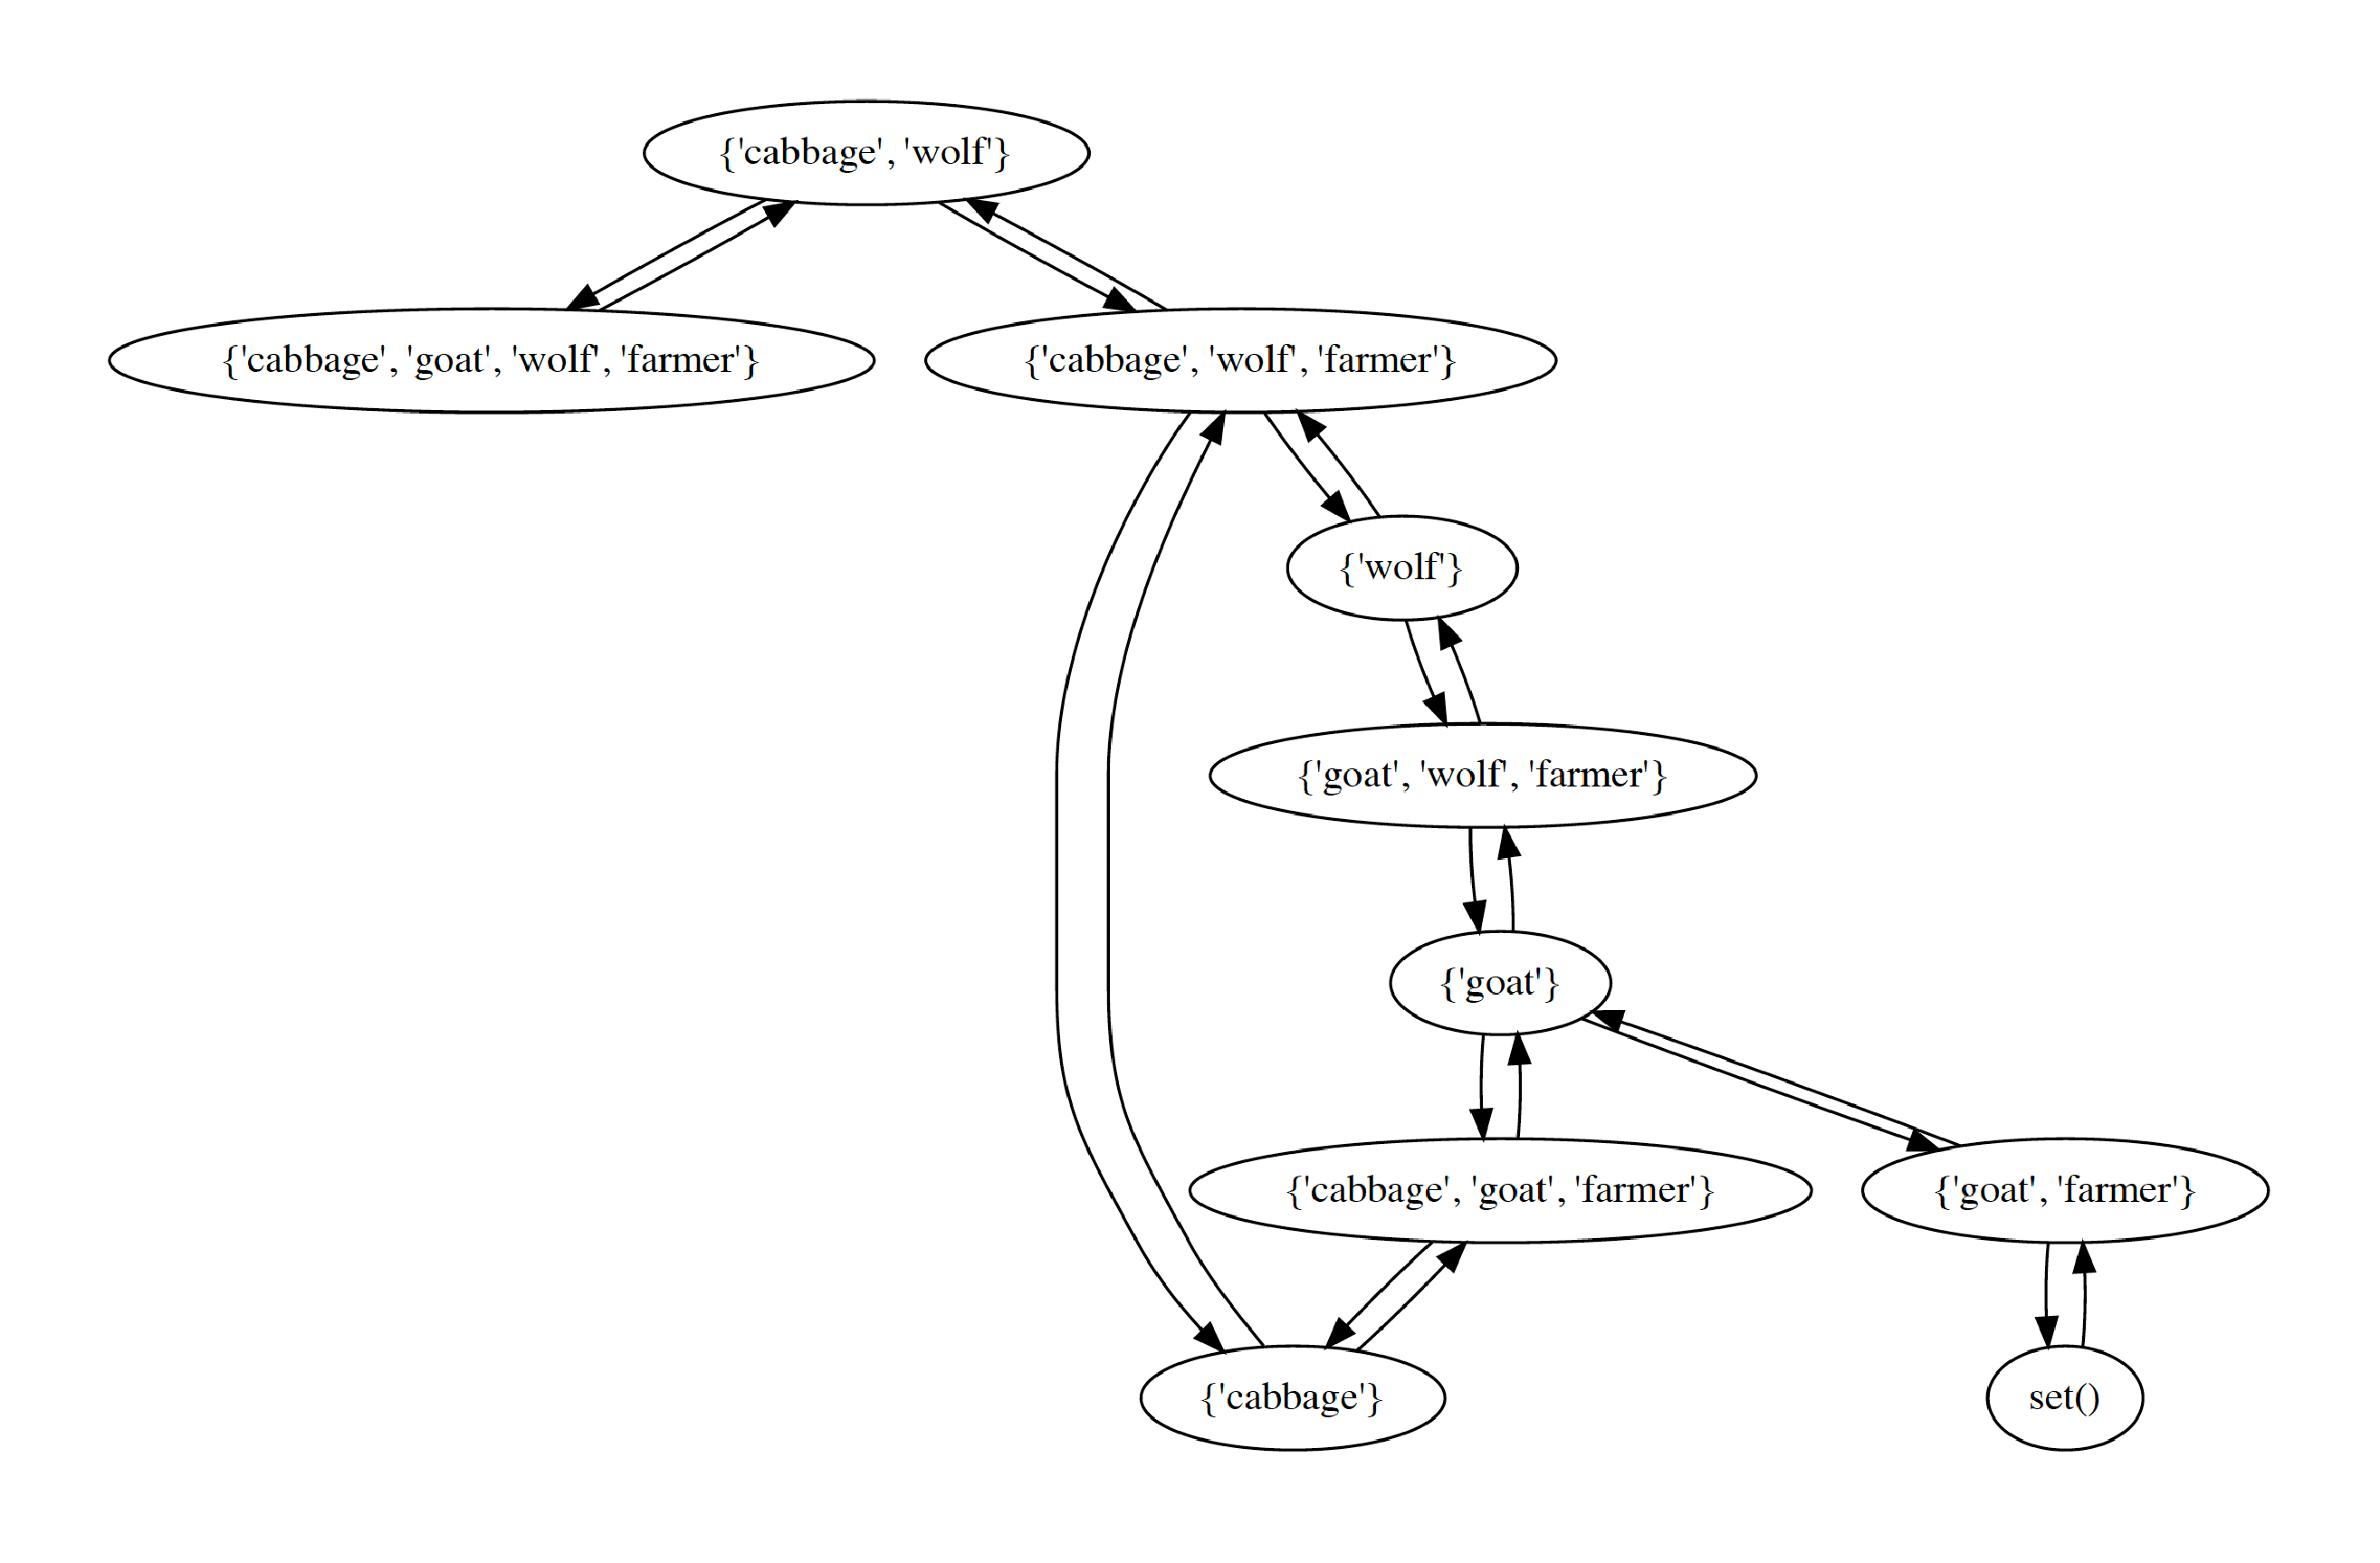
\epsfig{file=Figures/wolf-goat-cabbage, scale=0.4}

  \caption{The relation \texttt{R} shown as a directed graph.}
  \label{fig:wolf-goat-cabbage.pdf}
\end{figure}



\noindent
Figure \ref{fig:wolf-goat-cabbage.pdf} on page \pageref{fig:wolf-goat-cabbage.pdf} displays the relation $R$ graphically.
Figure \ref{fig:wolf-ziege} on page \pageref{fig:wolf-ziege} shows the program
\href{https://github.com/karlstroetmann/Logic/blob/master/Python/wolf-goat-cabbage.py}{\texttt{wolf-goat-cabbage.py}}
that combines the statements shown so far.  The solution computed by this program is shown in Figure
 \ref{fig:wolf-ziege-solution}.

\begin{figure}[!ht]
  \centering
\begin{minted}[ frame         = lines, 
                framesep      = 0.3cm, 
                numbers       = left,
                numbersep     = -0.2cm,
                bgcolor       = sepia,
                xleftmargin   = 0.3cm,
                xrightmargin  = 0.3cm,
              ]{python3}
    def problem(S):
        return ('farmer' not in S) and             \
               (('goat' in S and 'cabbage' in S) or   # goat eats cabbage
                ('wolf' in S and 'goat'    in S)   )  # wolf eats goat
    
    All   = frozenset({ 'farmer', 'wolf', 'goat', 'cabbage' })
    R1    = { (S, S - B) for S in States for B in power(S)
                         if S - B in States and 'farmer' in B and len(B) <= 2
            }
    R2    = { (S2, S1) for (S1, S2) in R1 }
    R     = R1 | R2
    start = All
    goal  = frozenset()
    Path  = findPath(start, goal, R)
\end{minted} 
\vspace*{-0.3cm}
\caption{Solving the wolf-goat-cabbage problem.}  
\label{fig:wolf-ziege}
\end{figure}


\begin{figure}[!ht]
  \centering
\begin{minted}[ frame         = lines, 
                framesep      = 0.3cm, 
                numbers       = left,
                numbersep     = -0.2cm,
                bgcolor       = sepia,
                xleftmargin   = 0.8cm,
                xrightmargin  = 0.8cm,
              ]{python3}
    {'cabbage', 'farmer', 'goat', 'wolf'}                                 {}
                             >>>> {'farmer', 'goat'} >>>> 
    {'cabbage', 'wolf'}                                   {'farmer', 'goat'}
                             <<<< {'farmer'} <<<< 
    {'cabbage', 'farmer', 'wolf'}                                   {'goat'}
                             >>>> {'farmer', 'wolf'} >>>> 
    {'cabbage'}                                   {'farmer', 'goat', 'wolf'}
                             <<<< {'farmer', 'goat'} <<<< 
    {'cabbage', 'farmer', 'goat'}                                   {'wolf'}
                             >>>> {'cabbage', 'farmer'} >>>> 
    {'goat'}                                   {'cabbage', 'farmer', 'wolf'}
                             <<<< {'farmer'} <<<< 
    {'farmer', 'goat'}                                   {'cabbage', 'wolf'}
                             >>>> {'farmer', 'goat'} >>>> 
    {}                                 {'cabbage', 'farmer', 'goat', 'wolf'}
\end{minted} 
\vspace*{-0.3cm}
\caption{A schedule for the agricultural economist.}  
\label{fig:wolf-ziege-solution}
\end{figure}
\pagebreak
\vspace*{\fill}



\section{Symbolic Differentiation}
\index{symbolic differentiation}
In this section we will develop a program that reads an arithmetic expression like the string
\\[0.2cm]
\hspace*{1.3cm}
\texttt{\symbol{34}x * exp(x)\symbol{34}},
\\[0.2cm]
interprets this string as describing the real valued function 
\\[0.2cm]
\hspace*{1.3cm}
$x \mapsto x \cdot \exp(x)$, 
\\[0.2cm]
and then takes the derivative of this function with respect to the variable $x$.  In order to specify the input
of this program more clearly, we first define the notion of an \blue{arithmetic expression} inductively.
\begin{enumerate}
\item Every number $c \in \mathbb{R}$ is an arithmetic expression.
\item Every variable $v$ is an arithmetic expression.
\item If $s$ and $t$ are arithmetic expressions, then
      \\[0.2cm]
      \hspace*{1.3cm}
      $s + t$, \quad $s - t$, \quad $s * t$, \quad $s / t$, \quad and \quad $s \,\mathtt{**}\, t$
      \\[0.2cm]
      are arithmetic expressions.  Here $s \,\mathtt{**}\, t$ is interpreted as $s^t$.
      
\item If $e$ is an arithmetic expression, then both
      \\[0.2cm]
      \hspace*{1.3cm}
      $\exp(e)$ \quad and \quad $\ln(e)$
      \\[0.2cm]
      are arithmetic expressions.
\end{enumerate}
We want do implement a function \texttt{diff} that takes two arguments:
\begin{enumerate}
\item The first argument \texttt{expr} is an arithmetic expression.
\item The second argument \texttt{var} is the name of a variable.
\end{enumerate}
The function call \texttt{diff(expr, var)} will then compute the derivative of \texttt{expr} with respect to the variable \texttt{var}.  For example, the function call \texttt{diff(\symbol{34}x*exp(x)\symbol{34}, \symbol{34}x\symbol{34})} will compute the output
\\[0.2cm]
\hspace*{1.3cm}
\symbol{34}\texttt{1*exp(x) + x*exp(x)}\symbol{34}
\\[0.2cm]
because we have:
$$ \frac{\mathrm{d}\;}{\mathrm{d}x} \bigl( x \cdot \mathrm{e}^x \bigr) = 1 \cdot x + x \cdot \mathrm{e}^x $$
It would be very tedious to \blue{represent} arithmetic expressions as strings.  Instead, we will represent
arithmetic expressions as \blue{nested tuples}.  \index{nested tuple}
The notion of a \emph{nested tuple} is defined inductively:
\begin{itemize}
\item $\langle x_1, x_2, \cdots, x_n \rangle$ is a nested tuple if each of the components $x_i$ is either a
      number, a string, or is itself a nested tuple.
\end{itemize}
For example, the arithmetic expression ``\texttt{x*exp(x)}'' is represented as the nested tuple
\\[0.2cm]
\hspace*{1.3cm}
$\bigl\langle\texttt{\symbol{34}}*\texttt{\symbol{34}}, \texttt{\symbol{34}}x\texttt{\symbol{34}}, \langle \texttt{\symbol{34}}\mathtt{exp}\texttt{\symbol{34}}, \texttt{\symbol{34}}x\texttt{\symbol{34}} \rangle\bigr\rangle$.
\\[0.2cm]
In order to be able to convert string into nested tuples, we need a \blue{parser}.
\index{parser}
  A parser is a program that
takes a string as input and transforms this string into a nested tuple, which is then returned as a result.
I have implemented a parser in the file ``\texttt{exprParser.py}''.  The details of the implementation of this
parser will be discussed in the lecture on
\href{https://github.com/karlstroetmann/Algorithms/blob/master/Lecture-Notes/algorithms.pdf}{algorithms} in the
second semester..

\noindent
The function \texttt{diff} that is shown in Figure \ref{fig:diff.py} on page \pageref{fig:diff.py} is part
of the program
\href{https://github.com/karlstroetmann/Logic/blob/master/Python/diff.py}{\texttt{diff.py}}.
This function is called with one argument:
The argument \texttt{e} is an arithmetic expression.
The function \texttt{diff} interprets its argument \texttt{e} as a function of the variable
\texttt{x}.  We take the \href{https://en.wikipedia.org/wiki/Derivative}{derivative} of this
function with respect to the variable \texttt{x}.  For example, in order to compute the derivative of
the function
\\[0.2cm]
\hspace*{1.3cm}
$x \mapsto x^x$,
\\[0.2cm]
we can call the function  \texttt{diff} as follows:
\\[0.2cm]
\hspace*{1.3cm}
\texttt{diff(\symbol{34}x ** x\symbol{34})}.
\\[0.2cm]
Let us now discuss the implementation of the function \texttt{diff} in more detail.  
\begin{enumerate}
\item The lines 3 - 6 implement the rule: 
      $$\frac{\mathrm{d}\;}{\mathrm{d}x}\bigl(f(x) + g(x)\bigr) = \frac{\mathrm{d}\;}{\mathrm{d}x} f(x) + \frac{\mathrm{d}\;}{\mathrm{d}x} g(x)$$
\item Line 7 - 10 implement the rule:
      $$\frac{\mathrm{d}\;}{\mathrm{d}x}\bigl(f(x) - g(x)\bigr) = \frac{\mathrm{d}\;}{\mathrm{d}x} f(x) - \frac{\mathrm{d}\;}{\mathrm{d}x} g(x)$$      
\item Line 11 - 14 deals with the case where \texttt{e} is a product.  The 
      \href{https://en.wikipedia.org/wiki/Product\_rule}{product rule} is      
      $$ \frac{\mathrm{d}\;}{\mathrm{d}x}\bigl(f(x) \cdot g(x)\bigr) = \left(\frac{\mathrm{d}\;}{\mathrm{d}x} f(x)\right)\cdot g(x) + f(x) \cdot \left(\frac{\mathrm{d}\;}{\mathrm{d}x} g(x)\right)
      $$
\item Line 15 - 17 deals with the case where \texttt{e} is a quotient.  The
      \href{https://en.wikipedia.org/wiki/Quotient\_rule}{quotient rule} is
      $$ \frac{\mathrm{d}\;}{\mathrm{d}x}\left(\frac{f(x)}{g(x)}\right) = 
         \frac{\displaystyle\left(\frac{\mathrm{d}\;}{\mathrm{d}x} f(x)\right)\cdot g(x) - 
         f(x) \cdot \left(\frac{\mathrm{d}\;}{\mathrm{d}x} g(x)\right)}{g(x) \cdot g(x)}
      $$      
\item Line 19 - 21 deals with the case where \texttt{e} is a power.  Now in order to take the derivative of an
      expression of the form
      $$  f(x)^{g(x)} $$
      we first need to rewrite this expression using the following trick:
      $$ f(x)^{g(x)} = \exp\bigl(\ln\bigl(f(x)^{g(x)}\bigr)\bigr) = \exp\bigl(g(x) \cdot \ln(f(x))\bigr) $$
      Then, we can recursively call \texttt{diff} for this expression.  This works, because the function
      \texttt{diff} can deal with both the exponential function $x \mapsto \exp(x)$ and with the natural
      logarithm $x \mapsto \ln(x)$.  This rewriting is done in line 21.      
\item Line 22-25 deals with the case where \texttt{e} has the form 
      $$\ln\bigl(f(x)\bigr)$$  
      In order to take the derivative of this expression, we first need to know the derivative of the natural
      logarithm.  This derivative is given as     
      $$ \frac{\mathrm{d}\;}{\mathrm{d}x} \ln(x) = \frac{1}{x}$$
      Then, using the \href{https://en.wikipedia.org/wiki/Chain\_rule}{chain rule} we have that
      $$ \frac{\mathrm{d}\;}{\mathrm{d}x} \ln\bigl(f(x)\bigr) = \frac{\frac{\mathrm{d}\;}{\mathrm{d}x} f(x)}{f(x)}$$     
\item Line 26 - 29 deals with the case where \texttt{e} has the form $\exp\bigl(f(x)\bigr)$.  
      In order to take the derivative of this expression, we first need to know the derivative of the 
      \href{https://en.wikipedia.org/wiki/Exponential\_function}{exponential function}.  
      This derivative is given as 
      $$ \frac{\mathrm{d}\;}{\mathrm{d}x} \exp(x) = \exp(x)$$    
      Then, using the \href{https://en.wikipedia.org/wiki/Chain\_rule}{chain rule} we have that
      $$\frac{\mathrm{d}\;}{\mathrm{d}x} \exp\bigl(f(x)\bigr) = \left(\frac{\mathrm{d}\;}{\mathrm{d}x} f(x)\right) \cdot \exp\bigl(f(x)\bigr) $$
\item Line 30-31 deals with the case where \texttt{e} is a variable and happens to be the same variable as
      \texttt{x}.  This is checked using the condition    
      \texttt{e == x}.  As we have
      $$\frac{\mathrm{d}x}{\mathrm{d}x} = 1,$$
      the function \texttt{diff} returns \texttt{1} in this case.  
\item Otherwise, the expression is assumed to be a constant and hence we return 0.
\end{enumerate}


\begin{figure}[!ht]
\centering
\begin{minted}[ frame         = lines, 
                framesep      = 0.3cm, 
                firstnumber   = 1,
                numbers       = left,
                numbersep     = -0.2cm,
                bgcolor       = sepia,
                xleftmargin   = 0.8cm,
                xrightmargin  = 0.8cm,
              ]{python3}
    def diff(e):
        'differentiate the expressions e with respect to the variable x'
        if e[0] == '+':
            f , g  = e[1:]
            fs, gs = diff(f), diff(g)
            return ('+', fs, gs)
        if e[0] == '-':
            f , g  = e[1:]
            fs, gs = diff(f), diff(g)
            return ('-', fs, gs)
        if e[0] == '*':
            f , g  = e[1:]
            fs, gs = diff(f), diff(g)
            return ('+', ('*', fs, g), ('*', f, gs))
        if e[0] == '/':
            f , g  = e[1:]
            fs, gs = diff(f), diff(g)
            return ('/', ('-', ('*', fs, g), ('*', f, gs)), ('*', g, g))
        if e[0] == '**':
            f , g  = e[1:]
            return diff(('exp', ('*', g, ('ln', f))))
        if e[0] == 'ln':
            f  = e[1]
            fs = diff(f) 
            return ('/', fs, f)
        if e[0] == 'exp':
            f  = e[1]
            fs = diff(f) 
            return ('*', fs, e)
        if e == 'x':
            return '1'
        return 0                  
\end{minted}
\vspace*{-0.3cm}
\caption{A function for symbolic differentiation}
\label{fig:diff.py}
\end{figure}


In order to test this function we can implement a function \texttt{test} as shown in Figure \ref{fig:test-diff.py}.
Then the expression
\\[0.2cm]
\hspace*{1.3cm}
\texttt{diff(\symbol{34}x ** x\symbol{34})}
\\[0.2cm]
yields the result:
\\[0.2cm]
\hspace*{1.3cm}
d/dx x ** x = (1*ln(x) + x*1/x)*exp(x*ln(x))
\\[0.2cm]
This shows that
\\[0.2cm]
\hspace*{1.3cm}
$\ds \frac{\mathrm{d}\;}{\mathrm{d}x} x^x = \bigl(\ln(x) + 1\bigr) \cdot \exp\bigl(x \cdot \ln(x)\bigr) =
 \bigl(\ln(x) + 1\bigr) \cdot x^x
$.


\begin{figure}[!ht]
\centering
\begin{minted}[ frame         = lines, 
                framesep      = 0.3cm, 
                firstnumber   = 1,
                numbers       = left,
                numbersep     = -0.2cm,
                bgcolor       = sepia,
                xleftmargin   = 0.8cm,
                xrightmargin  = 0.8cm,
              ]{python3}
    import exprParser as ep

    def test(s):
        t = ep.ExprParser(s).parse()
        d = diff(t)
        print(f'd/dx {s} = {ep.toString(d)}')
\end{minted}
\vspace*{-0.3cm}
\caption{Testing symbolic differentiation.}
\label{fig:test-diff.py}
\end{figure}





%%% Local Variables:
%%% mode: latex
%%% TeX-master: "logic"
%%% End:

\chapter{Grenzen der Berechenbarkeit}
In jeder Disziplin der Wissenschaft wird die Frage gestellt, welche \blue{Grenzen} die
verwendeten Methoden haben.   Wir wollen daher in diesem Kapitel beispielhaft ein Problem
untersuchen, bei dem die Informatik an ihre Grenzen stößt.  Es handelt sich um das
\href{http://de.wikipedia.org/wiki/Halteproblem}{Halte-Problem}.  

\section{Das Halte-Problem}
Das \blue{Halte-Problem} ist die Frage, ob eine gegebene Funktion $f$ für eine bestimmte Eingabe $x$ 
\blue{terminiert}, ob also der Aufruf $f(x)$ ein Ergebnis liefert oder sich in eine Endlos-Schleife
verabschiedet.   Bevor wir formal beweisen, dass das Halte-Problem im Allgemeinen \blue{unlösbar} ist, wollen 
wir versuchen, anschaulich zu verstehen, warum dieses Problem schwer sein muss.  Dieser informalen
Betrachtung des Halte-Problems ist der nächste Abschnitt gewidmet.  Im Anschluss an diesen Abschluss
beweisen wir dann formal die \blue{Unlösbarkeit} des Halte-Problems. 

\subsection{Informale Betrachtungen zum Halte-Problem}


\begin{figure}[!ht]
\centering
\begin{Verbatim}[ frame         = lines, 
                  framesep      = 0.3cm, 
                  firstnumber   = 1,
                  labelposition = bottomline,
                  numbers       = left,
                  numbersep     = -0.2cm,
                  xleftmargin   = 0.8cm,
                  xrightmargin  = 0.8cm
                ]
    def legendre(n):
        k = n * n + 1;
        while k < (n + 1) ** 2:
            if is_prime(k):
                return True
            k += 1
        return False
    
    def is_prime(k):
        return divisors(k) == {1, k}    
    
    def divisors(k):
        return { t for t in range(1, k+1) if k % t == 0 }
    
    def find_counter_example():
        n = 2
        while True:
           if legendre(n):
               n = n + 1
           else:
               print(f'Eureka! No prime between {n}**2 and {n+1}**2!')
               return
\end{Verbatim} 
\vspace*{-0.3cm}
\caption{Eine Funktion zur Überprüfung der von Legendre aufgestellten Vermutung.}
\label{fig:legendre.stlx}
\end{figure}

Um zu verstehen, warum das Halte-Problem schwer ist, betrachten wir  
das in Abbildung \ref{fig:legendre.stlx} gezeigte Programm. 
Dieses Programm ist dazu gedacht, die
\href{http://de.wikipedia.org/wiki/Legendresche_Vermutung}{\emph{Legendresche Vermutung}} zu
überprüfen.  Der französische 
Mathematiker  \href{http://de.wikipedia.org/wiki/Adrien-Marie_Legendre}{Adrien-Marie Legendre} 
(1752 --- 1833) hatte vor etwa 200 Jahren die Vermutung 
aufgestellt, dass zwischen zwei Quadrat-Zahlen immer eine Primzahl liegt.  Die Frage, ob diese
Vermutung richtig ist, ist auch heute noch unbeantwortet.  Die in Abbildung \ref{fig:legendre.stlx}
definierte Funktion $\texttt{legendre}(n)$ überprüft für eine gegebene positive natürliche Zahl $n$,
ob zwischen $n^2$ und $(n+1)^2$ eine Primzahl liegt.  Falls dies, wie von Legendre vermutet, der
Fall ist, gibt die Funktion als Ergebnis \texttt{True} zurück, andernfalls wird \texttt{False}
zurück gegeben.  Die Funktion \texttt{legendre} ist mit Hilfe der Funktion \texttt{is\_prime} definiert.  Für
eine natürliche Zahl $k$ liefert $\mathtt{is\_prime}(k)$ genau dann den Wert \texttt{True} zurück, wenn $k$
eine Primzahl ist.  Dazu überprüft die Funktion $\mathtt{is\_prime}(k)$ ob die Menge der Teiler von $k$ mit der Menge
die Menge $\{1, k\}$ übereinstimmt.  Die Menge der Teiler wird mit Hilfe der Funktion \texttt{divisors} berechnet.

Abbildung \ref{fig:legendre.stlx} enthält darüber hinaus die Definition der Funktion
$\texttt{findCounterExample}(n)$, die versucht, für eine gegebene positive natürliche Zahl $n$ eine
Zahl $k \geq n$ zu finden, so dass zwischen $k^2$ und $(k+1)^2$ keine Primzahl liegt.  Die Idee bei
der Implementierung dieser Funktion ist einfach:  Zunächst überprüfen wir durch den Aufruf
$\texttt{legendre}(n)$, ob zwischen $n^2$ und $(n+1)^2$
eine Primzahl liegt.  Falls dies der Fall ist, untersuchen wir anschließend das Intervall von
$(n+1)^2$ bis $(n+2)^2$, dann das Intervall von 
$(n+2)^2$ bis $(n+3)^2$ und so weiter, bis wir schließlich eine Zahl $m$ finden, so dass zwischen
$m^2$ und $(m+1)^2$ keine Primzahl liegt.  Falls Legendre Recht hatte, werden wir nie ein solches
$k$ finden und in diesem Fall wird der Aufruf $\texttt{findCounterExample}(2)$ nicht terminieren. 

Nehmen wir nun an, wir hätten ein schlaues Programm, nennen wir es \texttt{stops}, das als Eingabe
eine \textsl{Python} Funktion $f$ und ein Argument $a$ verarbeitet und das uns die Frage, ob die Berechnung von $f(a)$
terminiert, beantworten kann.  Die Idee wäre, dass die Funktion \texttt{stops} die folgende Spezifikation erfüllt:
\\[0.2cm]
\hspace*{1.3cm}
$\texttt{stops}(f, a) = \texttt{true}$ \quad g.d.w. \quad der Aufruf $f(a)$ terminiert.
\\[0.2cm]
Falls der Aufruf $f(a)$ nicht terminiert,  sollte stattdessen $\texttt{stops}(f,a) = \texttt{false}$ gelten.
Wenn wir eine solche Funktion \texttt{stops} hätten, dann könnten wir 
\\[0.2cm]
\hspace*{1.3cm}
\texttt{stops(findCounterExample, 1)}
\\[0.2cm]
aufrufen und wüssten anschließend, ob die Vermutung von Legendre wahr ist oder nicht:  Wenn
\\[0.2cm]
\hspace*{1.3cm}
$\texttt{stops(findCounterExample, 1)} = \texttt{true}$
 \\[0.2cm]
ist, dann würde das heißen,
dass der Funktions-Aufruf $\texttt{findCounterExample}(1)$ terminiert.  Das passiert aber nur dann,
wenn ein Gegenbeispiel gefunden wird.  Würde der Aufruf 
\\[0.2cm]
\hspace*{1.3cm}
\texttt{stops(findCounterExample, 1)}
\\[0.2cm]
stattdessen den Wert  $\texttt{false}$ zurück liefern, so könnten wir schließen, dass der Aufruf \texttt{findCounterExample(1)}
nicht terminiert. Mithin würde die Funktion \texttt{findCounterExample} kein Gegenbeispiel finden und
damit wäre klar, dass die von Legendre aufgestellte Vermutung wahr ist.

Es gibt eine Reihe weiterer offener  mathematischer Probleme, die alle auf die Frage abgebildet
werden können, ob eine gegebene Funktion terminiert.  Daher zeigen die vorhergehenden Überlegungen,
dass es sehr nützlich wäre, eine Funktion wie \texttt{stops} zur Verfügung zu haben.  Andererseits
können wir an dieser Stelle schon ahnen, dass die Implementierung der Funktion \texttt{stops}
nicht ganz einfach sein kann.  

 
\subsection{Formale Analyse des Halte-Problems}
Wir werden in diesem Abschnitt beweisen, dass das Halte-Problem unlösbar ist.  Dazu führen
wir den Begriff einer \blue{Test-Funktion} ein.  

\begin{Definition}[Test-Funktion] 
Ein String $t$ ist genau dann eine \blue{Test-Funktion} mit Namen $f$, wenn $t$ 
 die Form \\[0.3cm]
\hspace*{1.3cm} \texttt{\symbol{34}\symbol{34}\symbol{34}}         \\
\hspace*{1.3cm} \texttt{def $f$(x):} \\
\hspace*{1.8cm} \textsl{body}        \\
\hspace*{1.3cm} \texttt{\symbol{34}\symbol{34}\symbol{34}}         \\[0.2cm]
hat und sich als \textsl{Python}-Funktion parsen lässt.  Die Variable \textsl{body} steht hier für den Rumpf
der Test-Funktion.  Die Menge der Test-Funktionen bezeichnen wir mit $T\!F$.  \eox
\end{Definition}

\noindent
\textbf{Beispiele}:  
\begin{enumerate}
\item $s_1$ := 
     \texttt{\symbol{34}\symbol{34}\symbol{34}}        \\
     \hspace*{0.8cm} \texttt{def zero(x):} \\
     \hspace*{1.65cm} \texttt{return 0}        \\
     \hspace*{0.8cm} \texttt{\symbol{34}\symbol{34}\symbol{34}}        \\[0.2cm]
      $s_1$ ist eine (sehr einfache) Test-Funktion mit dem Name \texttt{zero}.
\item $s_2$ := 
     \texttt{\symbol{34}\symbol{34}\symbol{34}}        \\
     \hspace*{0.8cm}  \texttt{def loop(x):} \\
     \hspace*{1.65cm} \texttt{while True:}        \\
     \hspace*{2.5cm}  \texttt{x = x + 1}        \\
     \hspace*{0.8cm}  \texttt{\symbol{34}\symbol{34}\symbol{34}}        \\[0.2cm]
      $s_2$ ist eine Test-Funktion mit dem Name \texttt{loop}.
\item $s_3$ := 
     \texttt{\symbol{34}\symbol{34}\symbol{34}}        \\
     \hspace*{0.8cm}  \texttt{def buggy(x):} \\
     \hspace*{1.65cm} \texttt{while True:}        \\
     \hspace*{2.5cm}  \texttt{++x}        \\
     \hspace*{0.8cm}  \texttt{\symbol{34}\symbol{34}\symbol{34}}        \\[0.2cm]
      $s_3$ ist keine Test-Funktion, denn da \textsl{Python} den Präfix-Operator
      ``\texttt{++}'' nicht unterstützt, lässt sich der String $s_3$  nicht fehlerfrei als \textsl{Python} 
      parsen.
\item $s_4$ := 
     \texttt{\symbol{34}\symbol{34}\symbol{34}}        \\
     \hspace*{0.8cm}  \texttt{def sum(x, y):} \\
     \hspace*{1.65cm} \texttt{while True:}        \\
     \hspace*{2.5cm}  \texttt{return x + y}        \\
     \hspace*{0.8cm}  \texttt{\symbol{34}\symbol{34}\symbol{34}}        \\[0.2cm]
      $s_4$ ist keine Test-Funktion, denn ein String ist nur dann eine Test-Funktion, wenn die durch den String
      definierte Funktion mit \blue{genau einen} Parameter aufgerufen wird.
\end{enumerate}
Um das Halte-Problem übersichtlicher formulieren zu können, führen wir noch vier
zusätzliche Notationen ein.
\begin{Notation}[\textsl{name}, $\leadsto$, $\downarrow$, $\uparrow$]
{\em
Ist $t$ eine Testfunktion mit Namen $f$, so schreiben wir 
\\[0.2cm]
\hspace*{1.3cm}
$\textsl{name}(t) = f$.
\\[0.2cm]
Ist $f$ der Name einer \textsl{Python}-Funktion, die $k$ Argumente verarbeitet und sind $a_1$, $\cdots$, $a_k$ mögliche
Argumente, mit denen wir diese Funktion aufrufen können,
so schreiben wir \\[0.3cm]
\hspace*{1.3cm} $f(a_1, \cdots, a_k) \leadsto r$ \\[0.3cm]
wenn der Aufruf $f(a_1, \cdots, a_k)$ das Ergebnis $r$ liefert.  Sind wir an dem Ergebnis
selbst nicht interessiert, sondern wollen nur angeben, dass ein Ergebnis existiert, so
schreiben wir \\[0.3cm]
\hspace*{1.3cm} $f(a_1, \cdots, a_k) \,\downarrow$ \\[0.3cm]
und sagen, dass der Aufruf $f(a_1, \cdots, a_k)$ \blue{terminiert}.
Terminiert der Aufruf $f(a_1, \cdots, a_k)$ nicht, so schreiben wir \\[0.3cm]
\hspace*{1.3cm} $f(a_1, \cdots, a_k) \,\uparrow$ \\[0.3cm]
und sagen, dass der Aufruf $f(a_1, \cdots, a_k)$ \blue{divergiert}.  Diese Notation
verwenden wir auch, wenn der Aufruf  $f(a_1, \cdots, a_k)$ mit einer Fehlermeldung abbricht.
\hspace*{\fill} $\Box$
}
\end{Notation}

\noindent
\textbf{Beispiele}: Legen wir die Funktions-Definitionen zugrunde, die wir im Anschluss an
die Definition des Begriffs der Test-Funktion gegeben haben, so gilt:
\begin{enumerate}
\item {\tt zero(1)} $\leadsto 0$
\item {\tt zero(1)} $\downarrow$
\item {\tt loop(0)} $\uparrow$
\end{enumerate} 

\noindent
Das \blue{Halte-Problem} für
\textsl{Python}-Funktionen ist die Frage, ob es eine \texttt{SetlX}-Funktion \\[0.1cm] 
\hspace*{1.3cm} 
$\texttt{stops := procedure}(t,\;a)\; \{\;\cdots\;\}$ \\[0.1cm]
gibt, die als Eingabe eine Testfunktion $t$ und einen String $a$ erhält und die folgende
Eigenschaft hat:
\begin{enumerate}
\item $t \not\in T\!F \quad\Leftrightarrow\quad \mathtt{stops}(t, a) \leadsto 2$.

      Der Aufruf \texttt{stops($t$, $a$)} liefert genau dann den Wert 2 zurück, 
      wenn $t$ keine Test-Funktion ist.
\item $t \in T\!F \,\wedge\, \textsl{name}(t) = f \,\wedge\, f(a)\downarrow \quad\Leftrightarrow\quad
       \mathtt{stops}(t, a) \leadsto 1$.

      Der Aufruf \texttt{stops($t$, $a$)} liefert genau dann den Wert 1 zurück,
      wenn $t$ eine Test-Funktion mit Namen $f$ ist und der Aufruf $f(a)$ terminiert.

\item $t \in T\!F  \,\wedge\, \textsl{name}(t) = f \,\wedge\, t(a)\uparrow \quad\Leftrightarrow\quad
       \mathtt{stops}(t, a) \leadsto 0$.

      Der Aufruf \texttt{stops($t$, $a$)} liefert genau dann den Wert 0 zurück,
      wenn $t$ eine Test-Funktion ist und der Aufruf $t(a)$ \underline{nicht} terminiert.
\end{enumerate}
Falls eine \textsl{Python}-Funktion \texttt{stops} mit den obigen Eigenschaften existiert, dann
sagen wir, dass das Halte-Problem für \textsl{Python} entscheidbar ist.

\begin{Theorem}[\href{http://de.wikipedia.org/wiki/Alan_Turing}{Alan Turing}, 1936]
{\em
  Das Halte-Problem ist unentscheidbar.
} 
\end{Theorem}

\noindent
\textbf{Beweis}:  Zunächst eine Vorbemerkung.  Um die Unentscheidbarkeit des
Halte-Problems nachzuweisen, müssen wir zeigen, dass etwas, nämlich eine Funktion mit
gewissen Eigenschaften nicht existiert.  Wie kann so ein Beweis überhaupt funktionieren?
Wie können wir überhaupt zeigen, dass irgendetwas nicht existiert?
Die einzige Möglichkeit zu zeigen, dass etwas nicht existiert ist indirekt:
Wir nehmen also an, dass eine Funktion \texttt{stops} existiert, die das Halte-Problem löst.
Aus dieser Annahme werden wir einen Widerspruch ableiten.  Dieser Widerspruch zeigt
uns dann, dass eine Funktion \texttt{stops} mit den gewünschten Eigenschaften nicht
existieren kann.
Um zu einem Widerspruch zu kommen, definieren wir den String \texttt{turing} wie in Abbildung
\ref{fig:turing-string} gezeigt.

\begin{figure}[!h]
  \centering
\begin{Verbatim}[ frame         = lines, 
                  framesep      = 0.3cm, 
                  labelposition = bottomline,
                  numbers       = left,
                  numbersep     = -0.2cm,
                  xleftmargin   = 0.8cm,
                  xrightmargin  = 0.8cm,
                  commandchars  = \\\{\},
                ]
    turing = """
             def alan(x):
                 result = stops(x, x)
                 if result == 1:
                     while True:
                         print("... looping ...")
                 return result
             """ 
\end{Verbatim}
  \vspace*{-0.3cm}
  \caption{Die Definition des Strings \texttt{turing}.}
  \label{fig:turing-string}
\end{figure}

Mit dieser Definition ist klar, dass \texttt{turing} eine Test-Funktion mit Namen \texttt{alan} ist: \\[0.3cm]
\hspace*{1.3cm} $\texttt{turing} \in T\!F$ \quad und \quad $\textsl{name}(\texttt{turing}) = \texttt{alan}$. 
\\[0.3cm]
Damit sind wir in der Lage, den String \texttt{turing} als Eingabe der Funktion \texttt{stops}
zu verwenden.  Wir betrachten nun den folgenden Aufruf: \\[0.3cm]
\hspace*{1.3cm} \texttt{stops(\texttt{turing}, \texttt{turing});} \\[0.3cm]
Da \texttt{turing} eine Test-Funktion mit dem Namen \texttt{alan} ist und der Aufruf von \texttt{alan} mit dem Argument \texttt{turing}
auch nicht zu einem Fehler führen darf, können nur zwei Fälle auftreten:
\\[0.1cm]
\hspace*{1.3cm} 
$\texttt{stops(\texttt{turing}, \texttt{turing})} \leadsto 0 \quad \vee\quad
 \texttt{stops(\texttt{turing}, \texttt{turing})} \leadsto 1$. \\[0.1cm]
Diese beiden Fälle analysieren wir nun im Detail:
\begin{enumerate}
\item $\texttt{stops(\texttt{turing}, \texttt{turing})} \leadsto 0$. 

      Nach der Spezifikation von \texttt{stops} bedeutet dies \\[0.1cm]
      \hspace*{1.3cm} $\texttt{alan}(\texttt{turing}) \uparrow$ \\[0.1cm]
      Schauen wir nun, was wirklich beim Aufruf \texttt{alan(turing)} passiert:
      In Zeile 2 erhält die Variable \texttt{result} den Wert 0 zugewiesen.  In Zeile 3
      wird dann getestet, ob \texttt{result} den Wert 1 hat.  Dieser Test schlägt fehl.
      Daher wird der Block der \texttt{if}-Anweisung nicht ausgeführt und die Funktion liefert als
      nächstes in Zeile 8 den Wert 0 zurück.  Insbesondere terminiert der Aufruf also, im
      Widerspruch zu dem, was die Funktion \texttt{stops} behauptet hat. $\red{\lightning}$

      Damit ist der erste Fall ausgeschlossen.
\item  $\mathtt{stops}(\texttt{turing}, \texttt{turing}) \leadsto 1$. 

      Aus der Spezifikation der Funktion \texttt{stops} folgt, dass der Aufruf
      \texttt{alan(turing)} terminiert: \\[0.1cm]
      \hspace*{1.3cm} $\texttt{alan(turing)} \downarrow$ \\[0.1cm]
      Schauen wir nun, was wirklich beim Aufruf \texttt{alan(turing)} passiert:
      In Zeile 2 erhält die Variable \texttt{result} den Wert 1 zugewiesen.  In Zeile 3
      wird dann getestet, ob \texttt{result} den Wert 1 hat.  Diesmal gelingt der Test.
      Daher wird der Block der \texttt{if}-Anweisung ausgeführt.  Dieser Block
      besteht aber nur aus einer Endlos-Schleife, aus der wir nie wieder zurück kommen.
      Das steht im Widerspruch zu dem, was die Funktion \texttt{stops} behauptet hat.
      $\red{\lightning}$

      Damit ist der zweite Fall ausgeschlossen.
\end{enumerate}
Insgesamt haben wir also in jedem Fall einen Widerspruch erhalten.  
Damit muss die Annahme, dass die \textsl{Python}-Funktion \texttt{stops}
das Halte-Problem löst, falsch sein, denn diese Annahme ist die Ursache für die Widersprüche, die
wir erhalten haben.  Insgesamt haben wir daher gezeigt, dass es keine \textsl{Python}-Funktion
geben kann, die das Halte-Problem löst. \hspace*{\fill} $\Box$
\vspace*{0.3cm}

\noindent
\textbf{Bemerkung}:
Der Nachweis, dass das Halte-Problem unlösbar ist, wurde 1936 von Alan Turing (1912 -- 1954)
\cite{turing:36} erbracht.  Turing hat das Problem damals natürlich nicht für die Sprache
\textsl{Python} gelöst, sondern für die heute nach ihm benannten
\href{https://de.wikipedia.org/wiki/Turingmaschine}{Turing-Maschinen}.   
Eine Turing-Maschine ist abstrakt gesehen nichts anderes als eine Beschreibung eines
Algorithmus.  Turing hat also gezeigt, dass es keinen Algorithmus gibt, der entscheiden
kann, ob ein gegebener anderer Algorithmus terminiert.
\vspace*{0.3cm}

\noindent
\textbf{Bemerkung}:
An dieser Stelle können wir uns fragen, ob es vielleicht eine andere Programmier-Sprache
gibt, in der wir das Halte-Problem dann vielleicht doch lösen könnten.  
Wenn es in dieses Programmier-Sprache Prozeduren, \texttt{if}-Verzweigungen und
\texttt{while}-Schleifen gibt, und wenn wir dort 
Programm-Texte als Argumente von Funktionen übergeben können, dann ist leicht zu sehen,
dass der obige Beweis der 
Unlösbarkeit des Halte-Problems sich durch geeignete syntaktische Modifikationen auch auf
die andere Programmier-Sprache übertragen lässt.


\section{Unlösbarkeit des Äquivalenz-Problems}
Es gibt noch eine ganze Reihe anderer Funktionen, die nicht berechenbar sind.  In der
Regel werden wir den Nachweis, dass eine bestimmt Funktion nicht berechenbar ist, indirekt führen
und annehmen, dass die gesuchte Funktion doch berechenbar ist.  Unter dieser Annahme
konstruieren wir dann eine Funktion, die das Halte-Problem löst, was im Widerspruch zu der Unlösbarkeit
des Halte-Problems steht.
Dieser Widerspruch zwingt uns zu der Folgerung, dass die gesuchte Funktion nicht berechenbar ist.
Wir werden dieses Verfahren an einem Beispiel demonstrieren.  Vorweg benötigen wir aber
noch eine Definition.

\begin{Definition}[$\simeq$]  
Es seien $f_1$ und $f_2$ die Namen zwei \textsl{Python}-Funktionen und
  $a_1$, $\cdots$, $a_k$ seien Argumente, mit denen wir diese Funktionen füttern können. Wir definieren \\[0.1cm]
\hspace*{1.3cm} $t_1(a_1,\cdots,a_k) \simeq t_2(a_1,\cdots,a_k)$ \\[0.1cm]
g.d.w. einer der beiden folgen Fälle auftritt:
\begin{enumerate}
\item $f_1(a_1,\cdots,a_k)\uparrow \quad\wedge\quad f_2(a_1,\cdots,a_k)\uparrow$,

      beide Funktionen divergieren also für die gegebenen Argumente.
\item $\exists r: \Bigl(f_1(a_1,\cdots,a_k) \leadsto r \;\wedge\; f_2(a_1,\cdots,a_k) \leadsto r\Bigr)$,

      die beiden Funktionen liefern also für die gegebenen Argumente das gleiche Ergebnis.
\end{enumerate}
      In diesem Fall sagen wir, dass die beiden Funktions-Aufrufe 
      $f_1(a_1,\cdots,a_k) \simeq f_2(a_1,\cdots,a_k)$ \blue{partiell äquivalent} sind.  
      \qed
\end{Definition}

\noindent
Wir kommen jetzt zum \blue{Äquivalenz-Problem}.  Die Funktion $\texttt{equal}$ sei wie folgt definiert:
\\[0.2cm]
\hspace*{1.3cm} \texttt{def equal(t1, t2, a):} \\
\hspace*{2.2cm} \textsl{body}
\\[0.2cm]
Zusätzlich erfüllt \texttt{equal} die folgende Spezifikation:
\begin{enumerate}
\item $t_1 \not\in T\!F \;\vee\; t_2 \not\in T\!F \quad\Leftrightarrow\quad \mathtt{equal}(t_1, t_2, a) \leadsto 2$.
\item Falls 
  \begin{enumerate}
  \item $t_1 \in T\!F$ \quad und \quad $\textsl{name}(t_1) = f_1$,
  \item $t_2 \in T\!F$ \quad und \quad $\textsl{name}(t_2) = f_2$ \quad und
  \item $f_1(a) \simeq f_2(a)$
  \end{enumerate}
    gilt, dann muss gelten: \\[0.1cm]
   \hspace*{1.3cm}  $\mathtt{equal}(t_1, t_2, a) \leadsto 1$.
\item Ansonsten gilt \\[0.1cm]
      \hspace*{1.3cm} $\mathtt{equal}(t_1, t_2, a) \leadsto 0$.
\end{enumerate}
Wir sagen, dass eine Funktion, die der eben angegebenen Spezifikation genügt, das
\blue{Äquivalenz-Problem} löst.

\begin{Theorem}[Rice, 1953]
Das Äquivalenz-Problem ist unlösbar.  
\end{Theorem}

\noindent
\textbf{Beweis}:
Wir führen den Beweis indirekt und nehmen
an, dass es doch eine Implementierung der Funktion \texttt{equal} gibt, die das
Äquivalenz-Problem löst.  Wir betrachten die in Abbildung 
\ref{fig:stops} angegeben Implementierung der Funktion \texttt{stops}.


\begin{figure}[!h]
  \centering
\begin{Verbatim}[ frame         = lines, 
                  framesep      = 0.3cm, 
                  labelposition = bottomline,
                  numbers       = left,
                  numbersep     = -0.2cm,
                  xleftmargin   = 0.3cm,
                  xrightmargin  = 0.3cm
                ]
     def stops(t, a) {
         l = """
             def loop(x): 
                 while True:
                     x = 1
             """ 
         e = equal(l, t, a);
         if e == 2:
             return 2
         else:
             return 1 - e
\end{Verbatim}
  \vspace*{-0.3cm}
  \caption{Eine Implementierung der Funktion \texttt{stops}.}
  \label{fig:stops}
\end{figure}

Zu beachten ist, dass in Zeile 3 die Funktion \texttt{equal} mit einem String aufgerufen
wird, der eine Test-Funktion ist.  Diese 
Test-Funktion hat die
folgende Form:
\begin{verbatim}
            def loop(x): 
                 while True:
                     x = 1
\end{verbatim}
Es ist offensichtlich, dass diese Funktion für keine Eingabe terminiert.
Ist also das Argument $t$ eine Test-Funktion mit Namen $f$, so liefert die Funktion
\texttt{equal} immer dann den Wert 1, 
wenn $f(a)$ nicht terminiert, andernfalls muss sie den Wert 0 zurück geben.
Damit liefert die Funktion \texttt{stops} aber für eine Test-Funktion $t$ mit Namen $f$
und ein Argument $a$ genau dann 1, wenn der Aufruf $f(a)$ terminiert und würde folglich das Halte-Problem
lösen.  Das kann nicht sein, also kann es keine Funktion  \texttt{equal}
geben, die das Äquivalenz-Problem löst. 
\qed
\vspace*{0.3cm}

\noindent
Die Unlösbarkeit des Äquivalenz-Problems und vieler weiterer praktisch interessanter
Probleme folgen aus dem 1953 von Henry G.~Rice \cite{rice:53} bewiesenen
\href{http://de.wikipedia.org/wiki/Satz_von_Rice}{Satz von Rice}.

\section{Reflexion}
Beantworten Sie die folgenden Fragen.
\begin{enumerate}
\item Wie ist das Halteproblem definiert?
\item Versuchen Sie, die Definition der Funktion \texttt{turing} aus dem Gedächtnis aufzuschreiben und führen Sie
      dann den Nachweis, dass das Halteproblem nicht lösbar ist.
\item Wie haben wir das Äquivalenz-Problem definiert?
\item Haben Sie den Beweis der Unlösbarkeit des Äquivalenz-Problems verstanden?
\end{enumerate}


%%% Local Variables: 
%%% mode: latex
%%% TeX-master: "logic"
%%% ispell-local-dictionary: "deutsch8"
%%% End: 

\chapter{Aussagenlogik}
\section{Überblick}
Die Aussagenlogik beschäftigt sich mit der Verknüpfung \blue{einfacher Aussagen} durch
\blue{Junktoren}.  Dabei sind Junktoren\index{Junktor} Worte wie ``\blue{und}'', ``\blue{oder}'',
``\blue{nicht}'', ``\blue{wenn $\cdots$, dann}'', und ``\blue{genau dann, wenn}''.  Unter
\blue{einfachen Aussagen} verstehen wir Sätze, die 
\begin{itemize}
\item einen Tatbestand ausdrücken, der entweder wahr oder falsch ist und 
\item selber keine Junktoren enthalten.
\end{itemize}
Beispiele für einfache Aussagen sind
\begin{enumerate}
\item ``\textsl{Die Sonne scheint.}''
\item ``\textsl{Es regnet.}''
\item ``\textsl{Am Himmel ist ein Regenbogen.}''
\end{enumerate}
Einfache Aussagen dieser Art bezeichnen wir auch als \blue{atomare}\index{atomare Aussage} Aussagen, weil sie
sich nicht weiter in 
Teilaussagen zerlegen lassen.  Atomare Aussagen lassen sich mit Hilfe der eben angegebenen Junktoren zu 
\blue{zusammengesetzten Aussagen}\index{zusammengesetzte Aussagen} verknüpfen.  Ein Beispiel für eine
zusammengesetzte Aussage wäre \\[0.2cm] 
\hspace*{1.3cm} \textsl{\blue{Wenn} die Sonne scheint \blue{und} es regnet, \blue{dann} ist ein Regenbogen am Himmel.} 
\hspace*{\fill} (1)
\\[0.2cm]
Die Aussage ist aus den drei atomaren Aussagen ``\textsl{Die Sonne scheint.}'', ``\textsl{Es regnet.}'', und
``\textsl{Am Himmel ist ein Regenbogen.}'' mit Hilfe der Junktoren ``\textsl{und}'' und
``\textsl{wenn $\cdots$, dann}'' zusammen gesetzt worden.
Die Aussagenlogik untersucht, wie sich der Wahrheitswert zusammengesetzter Aussagen
aus dem Wahrheitswert der einzelnen Teilaussagen berechnen lässt.  Darauf
aufbauend wird dann gefragt, in welcher Art und Weise wir aus gegebenen Aussagen neue 
Aussagen folgern können.

Um die Struktur komplexerer Aussagen übersichtlich darstellen zu können, führen wir in der Aussagenlogik zunächst sogenannte
\blue{Aussage-Variablen} \index{Aussage-Variablen} ein.  Diese Variablen sind Namen, die für atomare Aussagen stehen.
Zusätzlich führen wir für die Junktoren \index{Junktor}
``\blue{nicht}'', ``\blue{und}'', ``\blue{oder}'', ``\blue{wenn, $\cdots$ dann}'', und 
``\blue{genau dann, wenn}'' die Symbole ``\blue{$\neg$}'', ``\blue{$\wedge$}'', ``\blue{$\vee$}'',
``\blue{$\rightarrow$}'' und ``\blue{$\leftrightarrow$}'' als Abkürzungen ein: 
\begin{enumerate}
\item $\neg a$ \index{$\neg a$}\quad\quad\ steht für \quad \blue{nicht} $a$ 
      \vspace*{-0.2cm}

\item $a \wedge b$ \index{$a \wedge b$}\,\quad\ steht für \quad $a$ \blue{und} $b$
      \vspace*{-0.2cm}

\item $a \vee b$ \index{$a \vee b$}\,\quad\ steht für \quad $a$ \blue{oder} $b$
      \vspace*{-0.2cm}

\item $a \rightarrow b$ \index{$a \rightarrow b$}  \quad steht für \quad \blue{wenn} $a$, \blue{dann} $b$
      \vspace*{-0.2cm}

\item $a \leftrightarrow b$ \index{$a \leftrightarrow b$} \quad steht für \quad  $a$ \blue{genau dann, wenn} $b$
\end{enumerate}
Aussagenlogische Formeln werden aus Aussage-Variablen mit Hilfe von Junktoren aufgebaut
und können beliebig komplex sein.  Die Aussage (1) können wir mit Hilfe der Junktoren kürzer als
 \\[0.2cm]
\hspace*{1.3cm}
$\texttt{SonneScheint} \wedge \texttt{EsRegnet} \rightarrow \texttt{Regenbogen}$ 
\\[0.2cm]
schreiben.  Hier haben wir $\texttt{SonneScheint}$, $\texttt{EsRegnet}$ und $\texttt{Regenbogen}$
als Aussage-Variablen verwendet.  Durch die Benutzung der Junktoren wird die logische Struktur der Aussage
klarer. 
Bestimmte aussagenlogische Formeln sind offenbar immer wahr, egal was
 wir für die einzelnen Teilaussagen einsetzen.  Beispielsweise ist eine Formel der Art
\\[0.2cm]
\hspace*{1.3cm}
$p \vee \neg p$
\\[0.2cm]
unabhängig von dem Wahrheitswert der Aussage $p$ immer wahr.  Eine aussagenlogische
Formel, die immer wahr ist, bezeichnen wir als eine \blue{Tautologie}\index{Tautologie}.  Andere
aussagenlogische Formeln sind nie wahr, beispielsweise ist die Formel
\\[0.2cm]
\hspace*{1.3cm}
$p \wedge \neg p$
\\[0.2cm]
immer falsch.  Eine Formel heißt \blue{erfüllbar}\index{erfüllbar}, wenn es wenigstens eine Möglichkeit
gibt, dass die Formel wahr wird, ansonsten heißt sie \blue{unerfüllbar}\index{unerfüllbar}  Im Rahmen der
Vorlesung werden wir verschiedene Verfahren 
entwickeln, mit denen es möglich ist zu entscheiden, ob eine aussagenlogische Formel eine
Tautologie ist oder ob sie erfüllbar ist.  Solche Verfahren spielen
in der Praxis eine wichtige Rolle.

Der Rest dieses Kapitels ist wir folgt strukturiert:
\begin{enumerate}
\item Wir diskutieren Anwendungen der Aussagenlogik.
\item Danach definieren wir formal, wie aussagenlogische Formeln aufgebaut sind.
  
      Formal sprechen wir in diesem Zusammenhang von der \blue{Syntax} aussagenlogische Formeln.
\item Anschließend diskutieren wir die Auswertung aussagenlogischer Formeln.
      Wir legen also fest, welchen Wahrheitswert eine aussagenlogische Formel unter einer gegebenen Belegung
      annimmt.  Wir zeigen in diesem Zusammenhang auch, wie die Auswertung aussagenlogischer Formeln sich in
      \textsl{Python}  implementieren lässt.

      Hier sprechen wir von der \blue{Semantik} der aussagenlogischen Formeln.
\item Danach führen wir die Begriffe der \blue{Tautologie} und der \blue{Erfüllbarkeit} einer aussagenlogischen
      Formel formal ein.
      \begin{enumerate}
      \item Eine aussagenlogische Formel ist eine \blue{Tautologie} genau dann, wenn Sie unter jeder möglichen
            Interpretation der aussagenlogischen Variablen wahr ist.
      \item Eine aussagenlogischen Formel ist \blue{erfüllbar} genau dann, wenn es eine Interpretation ihrer
            aussagenlogischen Variablen gibt, unter der die Formel wahr wird.
      \end{enumerate}
\item Wir diskutieren, wie sich aussagenlogische Formeln algebraisch umformen lassen und diskutieren
      in diesem Zusammenhang den Begriff der \blue{konjunktiven Normalform}.  Formeln, die in konjunktiver
      Normalform vorliegen, lassen sich auf dem Rechner leichter verarbeiten.
\item Anschließend diskutieren wir den \blue{Herleitungs-Begriff}.  Dabei geht es darum, aus Formeln,
      die als Axiome vorgegebenen sind, neue Formeln herzuleiten.
\item Schließlich stellen wir das Verfahren von \blue{Davis und Putnam} vor.  Mit diesem Verfahren lässt sich
      überprüfen, ob eine aussagenlogische Formel erfüllbar ist.  Als Anwendung zeigen wir, wie das
      8-Damen-Problem mit Hilfe des Verfahrens von Davis und Putnam gelöst werden kann.
\end{enumerate}

\section{Anwendungen der Aussagenlogik}
Die Aussagenlogik bildet nicht nur die Grundlage für die Prädikatenlogik, die wir im nächsten Kapitel
diskutieren werden, sondern sie hat auch wichtige prak\-tische Anwendungen.  Aus der großen Zahl der
industriellen Anwendungen möchte ich stellvertretend vier Beispiele nennen: 
\begin{enumerate}
\item Analyse und Design \blue{digitaler Schaltungen}.

      Komplexe digitale Schaltungen bestehen heute aus Milliarden von logischen Gattern.\footnote{Die Seite 
      \href{https://en.wikipedia.org/wiki/Transistor_count}{\texttt{https://en.wikipedia.org/wiki/Transistor\_count}}
      gibt einen Überblick über die Komplexität moderner Prozessoren.}
      Ein Gatter ist dabei, aus logischer Sicht betrachtet, ein Baustein, der einen
      der logischen Junktoren wie ``\blue{und}'', ``\blue{oder}'', ``\blue{nicht}'',
      etc.~auf elektronischer Ebene repräsentiert. 
  
      Die Komplexität solcher Schaltungen wäre ohne den Einsatz
      rechnergestützter Verfahren zur Verifikation nicht mehr beherrschbar.  Die
      dabei eingesetzten Verfahren sind Anwendungen der Aussagenlogik. 

      Eine ganz konkrete Anwendung ist der Schaltungs-Vergleich.  Hier werden zwei
      digitale Schaltungen als aussagenlogische Formeln dargestellt.
      Anschließend wird versucht, mit aussagenlogischen Mitteln die Äquivalenz dieser
      Formeln zu zeigen. Software-Werkzeuge, die für die Verifikation digitaler
      Schaltungen eingesetzt werden, kosten zum Teil mehr als $100\,000\,\symbol{36}$.
      Die Firma Magma bietet beispielsweise den \blue{Equivalence-Checker}
      \href{https://www.eetimes.com/document.asp?doc_id=1217672}{Quartz Formal} zum Preis
      von $150\,000\,
      \symbol{36}$ pro Lizenz an.  Eine solche Lizenz ist dann drei Jahre lang gültig.
\item Erstellung von \blue{Verschlussplänen} für die Weichen und Signale von Bahnhöfen.

      Bei einem größeren Bahnhof gibt es einige hundert Weichen und Signale, die ständig
      neu eingestellt werden müssen, um für die Züge sogenannte \blue{Fahrstraßen} zu
      realisieren.  Verschiedene Fahrstraßen dürfen sich aus Sicherheitsgründen nicht kreuzen.  
      Die einzelnen Fahrstraßen werden durch sogenannte \blue{Verschlusspläne} beschrieben.
      Die Korrektheit solcher Verschlusspläne kann durch aussagenlogische Formeln ausgedrückt werden.
\item Eine Reihe \blue{kombinatorischer Puzzles} lassen sich als aussagenlogische Formeln
      kodieren und können dann mit Hilfe aussagenlogischer Methoden gelöst werden.  Als ein
      Beispiel werden wir in der Vorlesung das 
      \href{https://en.wikipedia.org/wiki/Eight_queens_puzzle}{8-Damen-Problem} behandeln.  Dabei
      geht es um die Frage, ob 8 Damen so auf einem Schachbrett angeordnet werden können, dass
      keine der Damen eine andere Dame bedroht.
\end{enumerate}

\section{Formale Definition der aussagenlogischen Formeln}
Wir behandeln zunächst die \blue{Syntax} der Aussagenlogik und besprechen anschließend die
\blue{Semantik}.  Die \blue{Syntax}\index{Syntax} gibt an, wie Formeln geschrieben werden und wie sich Formeln zu
\blue{Beweisen} verknüpfen lassen.  Die \blue{Semantik}\index{Semantik} befasst sich mit der \blue{Bedeutung} der Formeln.
Nachdem wir die Semantik der aussagenlogischen Formeln mit Hilfe der Mengenlehre definiert haben, zeigen wir
anschließend, wie sich diese Semantik in \textsl{Python} implementieren lässt.

\subsection{Syntax der aussagenlogischen Formeln}
In diesem Abschnitt legen wir fest, was aussagenlogische Formeln sind:  Dazu werden wir aussagenlogische
Formeln als Menge von Strings definieren, wobei die Strings in der Menge bestimmte Eigenschaften haben müssen,
damit wir von aussagenlogischen Formeln sprechen können.

Zunächst betrachten wir eine Menge $\mathcal{P}$ \index{$\mathcal{P}$, Menge der Aussage-Variablen} von
sogenannten  \blue{Aussage-Variablen}\index{Aussage-Variablen} als gegeben. 
Typ\-ischerweise besteht $\mathcal{P}$ aus der Menge der kleinen lateinischen Buchstaben, die
zusätzlich noch indiziert sein dürfen.  Beispielsweise werden wir
\\[0.2cm]
\hspace*{1.3cm}
$p$, $q$, $r$, $p_1$, $p_2$, $p_3$
\\[0.2cm]
als Aussage-Variablen verwenden.
Aussagenlogische Formeln sind dann Wörter, die aus dem Alphabet
$$ 
  \mathcal{A} := \mathcal{P} \cup \bigl\{ \verum, \falsum, \neg, \vee, \wedge,
   \rightarrow, \leftrightarrow, (, ) \bigr\}
$$
gebildet werden.  Wir definieren die Menge der
\blue{aussagenlogischen Formeln}\index{aussagenlogische Formel}
\index{$\mathcal{F}$: Menge der aussagenlogischen Formeln}
$\mathcal{F}$ durch Induktion:
\begin{enumerate}
\item $\verum \in \mathcal{F}$ und $\falsum \in \mathcal{F}$.

      Hier steht $\verum$ \index{$\verum$, Verum} \index{Verum} für die Formel, die immer wahr ist, während $\falsum$
      \index{$\falsum$, Falsum} \index{Falsum} für die 
      Formel steht, die immer falsch ist.  Die Formel $\verum$ trägt den Namen
      \blue{Verum}\footnote{Verum ist das lateinische Wort für ``wahr''.},  für $\falsum$ sagen wir  
      \blue{Falsum}\footnote{Falsum ist das lateinische Wort für ``falsch''.}.
\item Ist $p \in \mathcal{P}$, so gilt auch $p \in \mathcal{F}$.

      Jede aussagenlogische Variable ist also auch eine aussagenlogische Formel.
\item Ist $f \in \mathcal{F}$, so gilt auch $\neg f \in \mathcal{F}$.

      Die Formel $\neg f$ \index{$\neg f$} bezeichnen wir auch als die \blue{Negation}\index{Negation} von $f$.
\item Sind $f_1, f_2 \in \mathcal{F}$, so gilt auch
      \begin{tabbing}
        $(f_1 \vee f_2) \in \mathcal{F}$ \index{$\vee$, oder} \hspace*{0.5cm} \= (\textsl{gelesen}: \quad \= $f_1$ oder $f_2$ \hspace*{2.5cm} \=
         auch: \blue{Disjunktion}\index{Disjunktion}\quad\= von $f_1$ und $f_2$), \\
        $(f_1 \wedge f_2) \in \mathcal{F}$ \index{$\wedge$, und} \> (\textsl{gelesen}: \> $f_1$ und $f_2$ \>
         auch: \blue{Konjunktion}\index{Konjunktion}\> von $f_1$ und $f_2$), \\
        $(f_1 \rightarrow f_2) \in \mathcal{F}$ \index{$\rightarrow$, wenn dann} \> (\textsl{gelesen}:       \> wenn $f_1$, dann $f_2$ \>
         auch: \blue{Implikation}\index{Implikation}\> von $f_1$ und $f_2$), \\
        $(f_1 \leftrightarrow f_2) \in \mathcal{F}$ \index{$\leftrightarrow$ genau dann, wenn} \> (\textsl{gelesen}:       \> $f_1$ genau dann, wenn $f_2$ \>
         auch: \blue{Bikonditional}\index{Bikonditional}\> von $f_1$ und $f_2$).            
      \end{tabbing}
\end{enumerate}
Die Menge $\mathcal{F}$ der aussagenlogischen Formeln ist nun die kleinste Teilmenge der aus dem Alphabet $\mathcal{A}$
gebildeten Wörter, welche die oben aufgelisteten Abschluss-Eigenschaften hat.

\example 
Es sei $\mathcal{P} := \{ p, q, r \}$. Dann gilt:
\begin{enumerate}
\item $p \in \mathcal{F}$,
\item $(p \wedge q) \in \mathcal{F}$,
\item $\Bigl(\bigl(\,(\neg p \rightarrow q) \vee (q \rightarrow \neg p)\,\bigr) \rightarrow r\Bigr) \in \mathcal{F}$.  \qed
\end{enumerate}

\noindent
Um Klammern zu sparen, vereinbaren wir die folgenden Regeln:
\begin{enumerate}
\item Äußere Klammern werden weggelassen, wir schreiben also beispielsweise \\[0.2cm]
      \hspace*{1.3cm} $p \wedge q$ \quad statt \quad $(p \wedge q)$.
\item Der Junktor $\neg$ bindet stärker als alle anderen Junktoren.
\item Die Junktoren  $\vee$ und $\wedge$ werden implizit links geklammert, d.h.~wir
      schreiben 
      \\[0.2cm]
      \hspace*{1.3cm} $p \wedge q \wedge r$ \quad statt \quad $(p \wedge q) \wedge r$.
      \\[0.2cm]
      Operatoren, die implizit nach \underline{links} geklammert werden, nennen wir
      \blue{links-assoziativ}\index{links-assoziativ}. 

      \underline{\color{red}Beachten} Sie, dass wir für diese Vorlesung vereinbaren, dass die Junktoren
      $\wedge$ und $\vee$ dieselbe Bindungsstärke haben.  Das ist anders als in der Sprache \textsl{Python},
      denn dort bindet der Operator ``\texttt{and}'' stärker als der Operator ``\texttt{or}''.
      In den Sprachen \texttt{C} und \textsl{Java} bindet der Operator ``\texttt{\&\&}'' ebenfalls stärker als
      der Operator ``\texttt{||}''. 
\item Der Junktor $\rightarrow$ wird implizit \underline{rechts} geklammert, d.h.~wir
      schreiben \\[0.2cm]
      \hspace*{1.3cm} $p \rightarrow q \rightarrow r$ \quad statt \quad $p \rightarrow (q \rightarrow r)$.
      \\[0.2cm]
      Operatoren, die implizit nach rechts geklammert werden, nennen wir
      \blue{rechts-assoziativ}\index{rechts-assoziativ}. 
\item Die Junktoren $\vee$ und $\wedge$ binden stärker als $\rightarrow$, wir schreiben
      also \\[0.2cm]
      \hspace*{1.3cm} $p \wedge q \rightarrow r$ \quad statt \quad $(p \wedge q) \rightarrow r$.
\item Der Junktor $\rightarrow$ bindet stärker als $\leftrightarrow$, wir schreiben
      also \\[0.2cm]
      \hspace*{1.3cm} $p \rightarrow q \leftrightarrow r$ \quad statt \quad $(p \rightarrow q) \leftrightarrow
      r$.
\item Beachten Sie, dass der Junktor $\leftrightarrow$ weder rechts- noch links-assoziativ ist.  Daher ist ein
      Ausdruck der Form
      \\[0.2cm]
      \hspace*{1.3cm}
      $p \leftrightarrow q \leftrightarrow r$
      \\[0.2cm]
      \underline{\red{undefiniert}} und muss geklammert werden.  Wenn Sie eine solche Formel in einem Buch sehen, ist dies
      in der Regel als Abkürzung für die Formel
      \\[0.2cm]
      \hspace*{1.3cm}
      $(p \leftrightarrow q) \wedge (q \leftrightarrow r)$
      \\[0.2cm]
      zu verstehen.  Wir werden diese Form der Abkürzung aber nicht verwenden.
\end{enumerate}

\remark
Wir werden im Rest dieser Vorlesung eine Reihe von Beweisen führen, bei denen es darum geht,
mathematische Aussagen über Formeln nachzuweisen.  Bei diesen Beweisen werden wir natürlich
ebenfalls aussagenlogische Junktoren verwenden.  Dabei entsteht dann die Gefahr, dass wir die Junktoren,
die wir in unseren Beweisen verwenden, mit den Junktoren, die in den aussagenlogischen Formeln
auftreten, verwechseln.  Um dieses Problem zu umgehen vereinbaren wir:
\begin{enumerate}
\item Innerhalb einer aussagenlogischen Formel wird der Junktor  
      ``\blue{nicht}'' als ``$\neg$''  geschrieben.
  
      Bei den Beweisen, die wir über aussagenlogische Formeln führen,
      schreiben wir den Junktor statt dessen als das Wort ``nicht''.

\item Innerhalb einer aussagenlogischen Formel wird der Junktor  
      ``\blue{und}'' als ``$\wedge$''  geschrieben.
  
      Bei den Beweisen, die wir über aussagenlogische Formeln führen,
      verwenden wir stattdessen das Wort ``und''.
\item Innerhalb einer aussagenlogischen Formel wird der Junktor  
      ``\blue{oder}'' als ``$\vee$''  geschrieben.
  
      Bei den Beweisen, die wir über aussagenlogische Formeln führen,
      verwenden wir stattdessen das Wort ``oder''.
\item Innerhalb einer aussagenlogischen Formel wird der Junktor  
      ``\blue{wenn $\cdots$,  dann}'' als ``$\rightarrow$''  geschrieben.
  
      Bei den Beweisen, die wir über aussagenlogische Formeln führen,
      verwenden wir stattdessen das Symbol ``$\Rightarrow$''.
\item Analog wird der Junktor ``\blue{genau dann, wenn}'' innerhalb einer aussagenlogischen Formel als
      ``$\leftrightarrow$'' geschrieben, aber wenn wir diesen Junktor als Teil eines Beweises verwenden,
      schreiben wir stattdessen ``$\Leftrightarrow$''. \eox      
\end{enumerate}


\subsection{Semantik der aussagenlogischen Formeln}
In diesem Abschnitt definieren wir die \blue{Semantik}\index{Semantik}, also die Bedeutung, aussagenlogischer Formeln.  Wir
legen also die \blue{Interpretation} oder auch \blue{Bedeutung} dieser Formeln fest.  Dazu ordnen wir den
aussagenlogischen Formeln \blue{Wahrheitswerte} zu.  Damit dies möglich ist, definieren wir
zunächst die Menge $\mathbb{B}$ der \blue{Wahrheitswerte}\index{Wahrheitswerte}:  \\[0.2cm] 
\hspace*{1.3cm} $\mathbb{B} := \{ \texttt{True}, \texttt{False} \}$. \\[0.2cm]
Damit können wir nun
den Begriff einer \blue{aussagenlogischen Interpretation} festlegen.

\begin{Definition}[Aussagenlogische Interpretation]
  Eine \blue{aussagenlogische Interpretation}\index{aussagenlogische Interpretation $\mathcal{I}$}
  \index{$\mathcal{I}$, aussagenlogische Interpretation} ist eine Funktion \\[0.2cm]
  \hspace*{1.3cm} $\mathcal{I}:\mathcal{P} \rightarrow \mathbb{B}$, \\[0.2cm]
  die jeder Aussage-Variablen $p\in \mathcal{P}$ einen Wahrheitswert $\mathcal{I}(p) \in \mathbb{B}$ zuordnet.
  \eox
\end{Definition}
Eine aussagenlogische Interpretation wird oft auch als \blue{Belegung}\index{Belegung} der
Aussage-Variablen mit Wahr\-heits-Werten bezeichnet.  

Eine aussagenlogische Interpretation $\mathcal{I}$ interpretiert die Aussage-Variablen.
Um nicht nur Variablen sondern auch aussagenlogische Formeln interpretieren zu können, 
benötigen wir eine
Interpretation der Junktoren ``$\neg$'', ``$\wedge$'', ``$\vee$'', ``$\rightarrow$'' und
``$\leftrightarrow$''.  Zu diesem Zweck definieren wir auf der Menge $\mathbb{B}$ der Wahr\-heits-Werte
Funktionen
$\circneg$, $\circwedge$, $\circvee$, $\circright$ und $\circleftright$,
mit deren Hilfe wir die aussagenlogischen Junktoren interpretieren können:
\begin{enumerate}
\item $\circneg: \mathbb{B} \rightarrow \mathbb{B}$ \index{$\circneg$}
\item $\circwedge: \mathbb{B} \times \mathbb{B} \rightarrow \mathbb{B}$ \index{$\circwedge$}
\item $\circvee: \mathbb{B} \times \mathbb{B} \rightarrow \mathbb{B}$ \index{$\circvee$}
\item $\circright: \mathbb{B} \times \mathbb{B} \rightarrow \mathbb{B}$ \index{$\circright$}
\item $\circleftright: \mathbb{B} \times \mathbb{B} \rightarrow \mathbb{B}$ \index{$\circleftright$}
\end{enumerate}
Wir könnten die Funktionen $\circneg$, $\circwedge$, $\circvee$, $\circright$ und $\circleftright$ am
einfachsten durch die folgende \blue{Wahrheits-Tafel} \index{Wahrheits-Tafel} (Tabelle
\ref{tab:aussagen-logik}) definieren:   


\begin{table}[!ht]
  \centering
\framebox{
  \begin{tabular}{|l|l||l|l|l|l|l|}
\hline
   $p$            & $q$             & $\circneg\;(p)$ & $\circvee\;(p, q)$ & $\circwedge\;(p, q)$ & $\circright\;(p, q)$ & $\circleftright\;(p, q)$
   \\
\hline
\hline
   \texttt{True}  & \texttt{True}   & \texttt{False}  & \texttt{True}  & \texttt{True}  & \texttt{True}     & \texttt{True}  \\
\hline
   \texttt{True}  & \texttt{False}  & \texttt{False}  & \texttt{True}  & \texttt{False} & \texttt{False}    & \texttt{False}  \\
\hline
   \texttt{False} & \texttt{True}   & \texttt{True}   & \texttt{True}  & \texttt{False} & \texttt{True}     & \texttt{False} \\
\hline
   \texttt{False} & \texttt{False}  & \texttt{True}   & \texttt{False} & \texttt{False} & \texttt{True}     & \texttt{True}  \\
\hline
  \end{tabular}}
  \caption{Interpretation der Junktoren}
  \label{tab:aussagen-logik}
\end{table}
Nun können wir den Wahrheits-Wert, den eine aussagenlogische Formel $f$ unter einer gegebenen
aussagenlogischen Interpretation $\mathcal{I}$ annimmt, durch Induktion nach dem Aufbau
der Formel $f$ definieren.  Wir werden diesen Wert mit $\widehat{\mathcal{I}}(f)$ \index{$\widehat{\mathcal{I}}(f)$}
bezeichnen.  Wir setzen:
\begin{enumerate}
\item $\widehat{\mathcal{I}}(\falsum) := \texttt{False}$.
\item $\widehat{\mathcal{I}}(\verum) := \texttt{True}$.
\item $\widehat{\mathcal{I}}(p) := \mathcal{I}(p)$ für alle $p \in \mathcal{P}$.
\item $\widehat{\mathcal{I}}(\neg f) := \circneg\;\bigl(\widehat{\mathcal{I}}(f)\bigr)$ für alle $f \in \mathcal{F}$.
\item $\widehat{\mathcal{I}}(f \wedge g) := \circwedge\;\bigl(\widehat{\mathcal{I}}(f), \widehat{\mathcal{I}}(g)\bigr)$ 
      für alle $f, g \in \mathcal{F}$.
\item $\widehat{\mathcal{I}}(f \vee g) := \circvee\;\bigl(\widehat{\mathcal{I}}(f), \widehat{\mathcal{I}}(g)\bigr)$ 
      für alle $f, g \in \mathcal{F}$.
\item $\widehat{\mathcal{I}}(f \rightarrow g) := \circright\;\bigl(\widehat{\mathcal{I}}(f), \widehat{\mathcal{I}}(g)\bigr)$ 
      für alle $f, g \in \mathcal{F}$.
\item $\widehat{\mathcal{I}}(f \leftrightarrow g) := \circleftright\;\bigl(\widehat{\mathcal{I}}(f), \widehat{\mathcal{I}}(g)\bigr)$ 
      für alle $f, g \in \mathcal{F}$.
\end{enumerate}
Um die Schreibweise nicht übermäßig kompliziert werden zu lassen, unterscheiden wir in
Zukunft nicht  mehr zwischen der Funktion $\widehat{\mathcal{I}}$ und der Funktion $\mathcal{I}$, wir werden das Hütchen über dem
$\mathcal{I}$ also weglassen.

\noindent
\textbf{Beispiel}: Wir zeigen, wie sich der Wahrheits-Wert der Formel
$$  (p \rightarrow q) \rightarrow (\neg p \rightarrow q) \rightarrow q $$
für die aussagenlogische Interpretation $\mathcal{I}$, die durch 
$\mathcal{I}(p) = \texttt{True}$ und $\mathcal{I}(q) = \texttt{False}$ definiert ist,
berechnen lässt: 
\\[0.2cm]
\hspace*{1.3cm}
$
  \begin{array}[b]{lcl}
   \mathcal{I}\Bigl( (p \rightarrow q) \rightarrow (\neg p \rightarrow q) \rightarrow q  \Bigr) 
   & = &  \circright\Bigl( \mathcal{I}\bigl( (p \rightarrow q) \bigr),\, \mathcal{I}\bigl((\neg p \rightarrow q) \rightarrow q\bigr) \Bigr) \\[0.2cm]
   & = & \circright\Bigl( \circright\bigl( \mathcal{I}(p), \mathcal{I}(q) \bigr),\, \mathcal{I}\bigl((\neg p \rightarrow q) \rightarrow q\bigr) \Bigr) \\[0.2cm]
   & = & \circright\Bigl( \circright\bigl( \texttt{True}, \texttt{False} \bigr),\, \mathcal{I}\bigl((\neg p \rightarrow q) \rightarrow q\bigr) \Bigr) \\[0.2cm]
   & = & \circright\Bigl( \texttt{False}, \, \mathcal{I}\bigl((\neg p \rightarrow q) \rightarrow q\bigr) \Bigr) \\[0.2cm]
   & = & \texttt{True} 
  \end{array}
$ \eox
\\[0.2cm]
Beachten Sie, dass wir bei der Berechnung gerade soviele Teile der Formel ausgewertet
haben, wie notwendig waren, um den Wert der Formel zu bestimmen.  Trotzdem ist die
eben durchgeführte Rechnung für die Praxis zu umständlich.  Stattdessen wird der Wert
einer Formel direkt mit Hilfe der Tabelle \ref{tab:aussagen-logik} auf Seite
\pageref{tab:aussagen-logik} berechnet.  Wir zeigen exemplarisch, wie wir den
Wahrheits-Wert der Formel
$$  (p \rightarrow q) \rightarrow (\neg p \rightarrow q) \rightarrow q $$
für beliebige Belegungen $\mathcal{I}$ über diese Tabelle berechnen können.
 Um nun die Wahrheitswerte 
dieser Formel unter einer gegebenen Belegung der Aussage-Variablen bestimmen zu können,
 bauen wir eine  Tabelle auf, die für jede in der Formel
auftretende Teilformel eine Spalte enthält.  Tabelle \ref{tab:tautologie} auf Seite
\pageref{tab:tautologie} zeigt die entstehende Tabelle.
\begin{table}[!ht]
  \centering
\framebox{
  \begin{tabular}{|l|l|l|l|l|l|l|}
\hline
   $p$ & $q$ & $\neg p$ & $p \rightarrow q$ & $\neg p \rightarrow q$ & $(\neg p \rightarrow q) \rightarrow q$ & $ (p \rightarrow q) \rightarrow (\neg p \rightarrow q) \rightarrow q$
   \\
\hline
\hline
   \texttt{True}  & \texttt{True}  & \texttt{False} & \texttt{True}  & \texttt{True}  & \texttt{True}     & \texttt{True}  \\
\hline
   \texttt{True}  & \texttt{False} & \texttt{False} & \texttt{False}  & \texttt{True} & \texttt{False}    & \texttt{True}  \\
\hline
   \texttt{False} & \texttt{True}  & \texttt{True}  & \texttt{True}  & \texttt{True} & \texttt{True}     & \texttt{True} \\
\hline
   \texttt{False} & \texttt{False} & \texttt{True}  & \texttt{True} & \texttt{False} & \texttt{True}     & \texttt{True}  \\
\hline
  \end{tabular}}
  \caption{Berechnung der Wahrheitswerte von $(p \rightarrow q) \rightarrow (\neg p \rightarrow q) \rightarrow q$}
  \label{tab:tautologie}
\end{table}

Betrachten wir die letzte Spalte der Tabelle, so sehen wir, dass dort immer der Wert
\texttt{True} auftritt.  Also liefert die Auswertung der Formel
$(p \rightarrow q) \rightarrow (\neg p \rightarrow q) \rightarrow q $
für jede aussagenlogische Belegung $\mathcal{I}$ den Wert \texttt{True}.  
Eine Formel, die immer wahr ist, wird als \href{https://en.wikipedia.org/wiki/Tautology_(logic)}{Tautologie} bezeichnet.

Wir erläutern die Aufstellung dieser Tabelle anhand der zweiten Zeile.  In dieser Zeile sind zunächst die
aussagenlogischen Variablen $p$ auf \texttt{True} und $q$ auf \texttt{False} gesetzt.  Bezeichnen wir die
aussagenlogische Interpretation mit $\mathcal{I}$, so gilt also\\[0.2cm]
\hspace*{1.3cm} $\mathcal{I}(p) = \texttt{True}$ und $\mathcal{I}(q) = \texttt{False}$. \\[0.2cm]
Damit erhalten wir folgende Rechnung:
\begin{enumerate}
\item $\mathcal{I}(\neg p) = \circneg\,(\mathcal{I}(p)) = \circneg\,( \texttt{True}) = \texttt{False}$
\item $\mathcal{I}(p \rightarrow q) = \circright\,(\mathcal{I}(p), \mathcal{I}(q)) = \circright\,(\texttt{True}, \texttt{False}) = \texttt{False}$
\item $\mathcal{I}(\neg p \rightarrow q) = \circright\bigl( \mathcal{I}(\neg p), \mathcal{I}(q)\bigr) = \circright(\texttt{False}, \texttt{False}) = \texttt{True}$
\item $\mathcal{I}\bigl((\neg p \rightarrow q) \rightarrow q\bigr) = 
          \circright\bigl( \mathcal{I}(\neg p \rightarrow q), \mathcal{I}(q) \bigr) = 
          \circright( \texttt{True}, \texttt{False} ) = \texttt{False}$
\item $\mathcal{I}\bigl((p \rightarrow q) \rightarrow  (\neg p \rightarrow q) \rightarrow q\bigr) = 
      \circright\bigl( \mathcal{I}(p \rightarrow q),  \mathcal{I}((\neg p \rightarrow q) \rightarrow q)\bigr) = 
       \circright\,( \texttt{False},  \texttt{False} ) = \texttt{True}$
\end{enumerate}
Für komplexe Formeln ist die Auswertung von Hand viel zu mühsam und
fehleranfällig, um praktikabel zu sein.  Wir zeigen deshalb später, wie
sich dieser Prozess mit Hilfe von \textsl{Python} automatisieren lässt.

\subsection{Extensionale und intensionale Interpretationen der Aussagenlogik}
\index{extensional} \index{intensional}
Die Interpretation der aussagenlogischen Junktoren ist rein \blue{extensional}:
Wenn wir den Wahrheitswert der Formel
\\[0.2cm]
\hspace*{1.3cm}
$\mathcal{I}(f \rightarrow g)$ 
\\[0.2cm]
berechnen wollen, so müssen wir die Details der Teilformeln $f$ und $g$ nicht kennen, es reicht,
wenn wir die Werte $\mathcal{I}(f)$ und $\mathcal{I}(g)$ kennen.   Das ist problematisch,
denn in der Umgangssprache hat der Junktor
``\textsl{wenn $\cdots$, dann}'' auch eine \blue{kausale} Bedeutung.  

Obwohl der folgende Satz mit der extensionalen Implikation 
\\[0.2cm]
\hspace*{1.3cm}
``\textsl{Wenn $3 \cdot 3 = 8$, dann schneit es.}''
\\[0.2cm]
als wahr interpretiert wird, erscheint er in ausgesprochener Form sinnlos.

Insofern ist die extensionale Interpretation des sprachlichen Junktors
``\textsl{wenn $\cdots$, dann}'' nur eine \blue{Approximation} der umgangssprachlichen Interpretation, die sich für die
Mathematik und die Informatik aber als ausreichend erwiesen hat.

Es gibt durchaus auch andere Logiken, in denen die Interpretation des Operators ``$\rightarrow$'' von der
hier gegebenen Definition abweicht.  Solche Logiken werden als
\href{https://en.wikipedia.org/wiki/Intensional_logic}{intensionale Logiken} bezeichnet.  Diese Logiken spielen
zwar in der Informatik auch eine Rolle, aber da die Untersuchung intensionaler Logiken wesentlich
aufwändiger ist als die Untersuchung der extensionalen Logik, werden wir uns auf die Analyse letzterer beschränken.

\subsection{Implementierung in \textsl{Python}} 
Um die bisher eingeführten Begriffe nicht zu abstrakt werden zu lassen,
entwickeln wir in \textsl{Python} ein Programm, mit dessen Hilfe sich Formeln
auswerten lassen.  
Jedes Mal, wenn wir ein Programm zur Berechnung irgendwelcher Werte entwickeln wollen,
müssen wir uns als erstes fragen, wie wir die Argumente der zu implementierenden Funktion und die
Ergebnisse dieser Funktion in der verwendeten Programmier-Sprache darstellen können.
In diesem Fall müssen wir uns also überlegen, wie wir eine
aussagenlogische Formel in \textsl{Python} repräsentieren können, denn die Ergebniswerte
\texttt{True} und \texttt{False} stehen ja als Wahrheitswerte unmittelbar zur Verfügung.
Zusammengesetzte Daten-Strukturen können in \textsl{Python} am einfachsten als
\blue{geschachtelte Tupel}\index{geschachtelte Tupel} dargestellt werden und das ist auch der Weg, den wir für
die aussagenlogischen Formeln beschreiten werden.  Ein geschachteltes Tupel ist dabei ein Tupel, dass
sowohl Strings als auch geschachtelte Tupel enthalten kann.  Beispiels\-weise ist
\\[0.2cm]
\hspace*{1.3cm}
\texttt{('$\wedge$', ('$\neg$', 'p'), 'q')}
\\[0.2cm]
ein geschachteltes Tupel, das die aussagenlogische Formel $\neg p \wedge q$ repräsentiert.

Wir legen die Repräsentation von aussagenlogischen Formeln nun formal dadurch fest, dass wir eine Funktion
\\[0.2cm]
\hspace*{1.3cm}
$\textsl{rep}: \mathcal{F} \rightarrow \textsl{Python}$
\\[0.2cm]
definieren, die einer aussagenlogischen Formel $f$ ein geschachteltes Tupel \index{geschachteltes Tupel}
$\textsl{rep}(f)$ zuordnet.  Diese Funktion definieren wir durch Induktion nach der Formel $f$:
\begin{enumerate}
\item $\verum$ wird repräsentiert durch das Tupel \texttt{('$\top$',)}.
      Dies ist möglich, da \texttt{'$\top$'} ein Unicode-Zeichen ist und Python die Verwendung von
      Unicode-Zeichen in Strings erlaubt.  Wir können diesen String alternativ in \textsl{Python} 
      auch in der Form
      \texttt{'\symbol{92}N\{up tack\}'} schreiben, denn ``\texttt{up tack}'' ist der Name des
      Unicode-Zeichens ``$\top$'' und ein Unicode Zeichen, das den Namen $u$ hat, kann in \textsl{Python}
      als \texttt{'\symbol{92}N\{$u$\}'} geschrieben werden.  Also haben wir
      \\[0.2cm]
      \hspace*{1.3cm}
      $\textsl{rep}(\verum) := \texttt{('\symbol{92}N\{up tack\}',)}$.
\item $\falsum$  wird repräsentiert durch das Tupel \texttt{('$\falsum$',)}.
      Das Unicode-Zeichen \texttt{'$\falsum$'} trägt den Namen \linebreak
      ``\texttt{down tack}''.
      Also haben wir
      \\[0.2cm]
      \hspace*{1.3cm}
      $\textsl{rep}(\falsum) := \texttt{('\symbol{92}N\{down tack\}',)}$.
\item Da aussagenlogische Variablen nichts anderes als Strings sind, können wir eine aussagen\-logische Variable
      durch sich selbst repräsentieren:
      \\[0.2cm]
      \hspace*{1.3cm}
      $\textsl{rep}(p) := p$ \quad für alle $p \in \mathcal{P}$.
\item Ist $f$ eine aussagenlogische Formel, so repräsentieren wir die Negation $\neg f$ als geschachteltes Tupel,
      bei dem wir das Unicode-Zeichen \texttt{'$\neg$'} an die erste Stelle setzen und anschließend
      rekursiv die Formel $f$ in ihre \textsl{Python}-Repräsentierung umwandeln.
      Der Name des Unicode-Zeichen \texttt{'$\neg$'} ist 
      ``\texttt{not sign}''.  Also haben wir
      \\[0.2cm]
      \hspace*{1.3cm} 
      $\textsl{rep}(\neg f) := \bigl(\texttt{'$\neg$'}, \textsl{rep}(f)\bigr)$.
\item Sind $f_1$ und $f_2$ aussagenlogische Formeln, so repräsentieren wir $f_1 \wedge f_2$ mit
      Hilfe des Unicode-Zeichens  \texttt{'$\wedge$'}, das den Namen 
      ``\texttt{logical and}'' hat:
      \\[0.2cm]
      \hspace*{1.3cm} 
      $\textsl{rep}(f \wedge g) := \bigl(\texttt{'$\wedge$'}, \textsl{rep}(f), \textsl{rep}(g)\bigr)$.
\item Sind $f_1$ und $f_2$ aussagenlogische Formeln, so repräsentieren wir $f_1 \vee f_2$ mit
      Hilfe des Unicode-Zeichens  \texttt{'$\vee$'}, das den Namen ``\texttt{logical or}'' hat:
      \\[0.2cm]
      \hspace*{1.3cm} 
      $\textsl{rep}(f \vee g) := \bigl(\texttt{'$\vee$'}, \textsl{rep}(f), \textsl{rep}(g)\bigr)$.
\item Sind $f_1$ und $f_2$ aussagenlogische Formeln, so repräsentieren wir $f_1 \rightarrow f_2$ mit
      Hilfe des Unicode-Zeichens  \texttt{'$\rightarrow$'}, das den Namen ``\texttt{rightwards arrow}'' hat:
      \\[0.2cm]
      \hspace*{1.3cm} 
      $\textsl{rep}(f \rightarrow g) := \bigl(\texttt{'$\rightarrow$'}, \textsl{rep}(f), \textsl{rep}(g)\bigr)$.
\item Sind $f_1$ und $f_2$ aussagenlogische Formeln, so repräsentieren wir $f_1 \leftrightarrow f_2$ mit
      Hilfe des Unicode-Zeichens  \texttt{'$\leftrightarrow$'}, das den Namen ``\texttt{left right arrow}'' hat:
      \\[0.2cm]
      \hspace*{1.3cm} 
      $\textsl{rep}(f \leftrightarrow g) := \bigl(\texttt{'$\leftrightarrow$'}, \textsl{rep}(f), \textsl{rep}(g)\bigr)$.
\end{enumerate}
Bei der Wahl der Repräsentation, mit der wir eine Formel in \textsl{Python} repäsentieren,
sind wir weitgehend frei.  Wir hätten oben sicher auch eine andere Repräsentation
verwenden können.  Eine gute Repräsentation sollte einerseits möglichst \blue{intuitiv} sein, andererseits ist
es auch wichtig, dass die Repräsentation für die zu entwickelnden Algorithmen \blue{adäquat}
ist.  Im Wesentlichen heißt dies, dass es einerseits einfach sein sollte, auf
die Komponenten einer Formel zuzugreifen, andererseits sollte es auch leicht sein,
die entsprechende Repräsentation zu erzeugen.

Als nächstes geben wir an, wie wir eine \blue{aussagenlogische Interpretation} in \textsl{Python}
darstellen.  Eine aussagenlogische Interpretation ist eine Funktion 
\\[0.2cm]
\hspace*{1.3cm} ${\cal I}: {\cal P} \rightarrow \mathbb{B}$ \\[0.2cm]
von der Menge der Aussage-Variablen ${\cal P}$ in die Menge der Wahrheitswerte 
$\mathbb{B}$.  Eine Möglichkeit eine solche aussagenlogische Interpretation darzustellen besteht
darin,  dass wir die Menge aller aussagenlogischen Variablen angeben, die unter der aussagenlogischen
Interpretation $\mathcal{I}$ den Wert \texttt{True} annehmen:
\\[0.2cm]
\hspace*{1.3cm}
$\textsl{rep}(\mathcal{I}) := \bigl\{ x \in \mathcal{P} \mid \mathcal{I}(x) = \texttt{True} \bigr\}$.
\\[0.2cm]
Damit können wir jetzt eine einfache Funktion implementieren, die den Wahrheitswert
einer aussagenlogischen Formel $f$ unter einer gegebenen aussagenlogischen
Interpretation ${\cal I}$ berechnet. Die Funktion
\texttt{evaluate}
ist in Abbildung \ref{fig:evaluate.py} auf Seite \pageref{fig:evaluate.py} gezeigt.
Die Funktion \texttt{evaluate} erwartet zwei Argumente:
\begin{enumerate}
\item Das erste Argument $F$ ist eine aussagenlogische Formel, die als geschachteltes Tupel dargestellt wird.
\item Das zweite Argument $I$ ist eine aussagenlogische Interpretation, die als Menge von aussagenlogischen Variablen
      dargestellt wird.  Für eine aussagenlogische Variable mit dem Namen $p$ können wir den Wert,
      der dieser Variablen durch $I$ zugeordnet wird, mittels des Ausdrucks ``$p \;\mathtt{in}\; I$'' berechnen.
\end{enumerate}

\begin{figure}[!ht]
  \centering
\begin{minted}[ frame         = lines, 
                framesep      = 0.3cm, 
                bgcolor       = sepia,
                numbers       = left,
                numbersep     = -0.2cm,
                xleftmargin   = 0.3cm,
                xrightmargin  = 0.3cm
               ]{python3}
    def evaluate(F, I):
        "Evaluate the propositional formula F using the interpretation I"
        if isinstance(F, str): # F is a propositional variable
            return F in I
        if F[0] == '⊤': return True
        if F[0] == '⊥': return False
        if F[0] == '¬': return not evaluate(F[1], I)
        if F[0] == '∧': return     evaluate(F[1], I) and evaluate(F[2], I)
        if F[0] == '∨': return     evaluate(F[1], I) or  evaluate(F[2], I)
        if F[0] == '→': return not evaluate(F[1], I) or  evaluate(F[2], I)
        if F[0] == '↔': return     evaluate(F[1], I) ==  evaluate(F[2], I)
\end{minted}
\vspace*{-0.3cm}
  \caption{Auswertung einer aussagenlogischen Formel}
  \label{fig:evaluate.py}
\end{figure} 

\noindent
Wir diskutieren jetzt die Implementierung der Funktion \texttt{evaluate()} Zeile für
Zeile:
\begin{enumerate}
\item In Zeile 3 betrachten wir den Fall, dass das Argument $F$ eine aussagenlogische
      Variable repräsentiert.  Dies erkennen wir daran, dass $F$ ein String ist.
      Die vordefinierte Funktion \texttt{isinstance} führt diese Überprüfung durch.

      In diesem Fall müssen wir wissen, ob die Variable $F$ ein Element der Menge $I$ ist, denn genau dann
      wird $F$ als wahr interpretiert.
\item Falls die Formel $F$ den Wert $\verum$ hat, so ist das Ergebnis der Auswertung unabhängig von der
      aussagenlogischen Interpretation $I$ immer \texttt{True}. 
      Um zu erkennen, ob $F$ die Formel $\verum$ repräsentiert, betrachten wir die erste Komponente
      des Tupels $F$ und überprüfen also, ob $F[0]$ das Zeichen \texttt{'$\verum$'} ist.
\item Falls die Formel $F$ den Wert $\falsum$ hat, so ist das Ergebnis der
      Auswertung unabhängig von der aussagenlogischen Interpretation $I$ immer \texttt{False}.
\item In Zeile 7 betrachten wir den Fall, dass $F$ die Form $\neg G$  hat.
      In diesem Fall werten wir erst $G$ unter der Belegung $I$ aus und negieren dann das Ergebnis.
\item In Zeile 8 betrachten wir den Fall, dass $F$ die Form 
      $G_1 \wedge G_2$ hat.
      In diesem Fall werten wir zunächst $G_1$ und $G_2$ unter der Belegung $I$ 
      aus und verknüpfen  das Ergebnis mit dem Operator ``\texttt{and}''.
\item In Zeile 9 betrachten wir den Fall, dass $F$ die Formel $G_1 \vee G_2$ repräsentiert.
      In diesem Fall werten wir zunächst $G_1$ und $G_2$ unter der Belegung $I$ 
      aus und verknüpfen  das Ergebnis mit dem Operator ``\texttt{or}''.
\item In Zeile 10 betrachten wir den Fall, dass $F$ die Form $G_1 \rightarrow G_2$ hat.
      In diesem Fall werten wir zunächst $G_1$ und $G_2$ unter der Belegung $I$ 
      aus und nutzen dann aus, dass die Formeln
      \\[0.2cm]
      \hspace*{1.3cm}
      $G_1 \rightarrow G_2$ \quad und \quad $\neg G_1 \vee G_2$
      \\[0.2cm]
      äquivalent sind.
\item In Zeile 11 führen wir die Auswertung einer Formel $F \leftrightarrow G$ darauf zurück, dass diese
      Formel genau dann wahr ist, wenn $F$ und $G$ den selben Wahrheitswert haben.
\end{enumerate}

\subsection{Eine Anwendung}
Wir betrachten eine spielerische Anwendung der Aussagenlogik.  Inspektor Watson wird zu
einem Juweliergeschäft gerufen, in das eingebrochen worden ist.
In der unmittelbaren Umgebung werden drei Verdächtige Aaron, Bernard und Caine festgenommen.
Die Auswertung der Akten ergibt folgendes:
\begin{enumerate}
\item Einer der drei Verdächtigen muss die Tat begangen haben: \\[0.2cm]
      \hspace*{1.3cm} 
      $f_1 := a \vee b \vee c$.
\item Wenn Aaron schuldig ist, so hat er genau einen Komplizen. 

      Diese Aussage zerlegen wir zunächst in zwei Teilaussagen:
      \begin{enumerate}
      \item Wenn Aaron schuldig ist, dann hat er mindestens einen Komplizen: \\[0.2cm]
            \hspace*{1.3cm} $f_2 := a \rightarrow b \vee c$ 
      \item Wenn Aaron schuldig ist, dann hat er höchstens einen Komplizen: \\[0.2cm]
           \hspace*{1.3cm} $f_3 := a \rightarrow \neg (b \wedge c)$
      \end{enumerate}
\item Wenn Bernard unschuldig ist, dann ist auch Caine unschuldig: \\[0.2cm]
      \hspace*{1.3cm} $f_4 :=  \neg b \rightarrow \neg c$ 
\item Wenn genau zwei schuldig sind, dann ist Caine einer von ihnen.

      Es ist nicht leicht zu sehen, wie sich diese Aussage aussagenlogisch
      formulieren lässt.  Wir behelfen uns mit einem Trick und überlegen uns, wann die
      obige Aussage falsch ist.  Wir sehen, die Aussage ist dann falsch,
      wenn Caine nicht schuldig ist und wenn gleichzeitig Aaron und Bernard schuldig sind.
      Damit lautet die Formalisierung der obigen Aussage: \\[0.2cm]
      \hspace*{1.3cm} $f_5 := \neg ( \neg c  \wedge a \wedge b )$ 
\item Wenn Caine unschuldig ist, ist Aaron schuldig. \\[0.2cm]
      \hspace*{1.3cm} $f_6 := \neg c \rightarrow a$
\end{enumerate}
Wir haben nun eine Menge $F = \{ f_1, f_2, f_3, f_4, f_5, f_6 \}$ von Formeln.
Wir fragen uns nun, für welche Belegungen $\mathcal{I}$ alle Formeln aus der Menge $F$ wahr werden.
Wenn es genau eine Belegung gibt, für die dies der Fall ist, dann liefert uns die
Belegung den oder die Täter.  Eine Belegung entspricht dabei 1-zu-1 der Menge der Täter.
Da es zu zeitraubend ist, alle Belegungen von Hand auszuprobieren,
schreiben wir besser ein Programm, das die notwendigen Berechnungen für uns durchführt.
Abbildung \ref{fig:Usual-Suspects.ipynb} zeigt das Programm
\href{https://github.com/karlstroetmann/Logic/blob/master/Python/Usual-Suspects.ipynb}{\texttt{Usual-Suspects.ipynb}}.
Wir diskutieren dieses Programm nun Zeile für Zeile.

\begin{figure}[!ht]
  \centering
\begin{minted}[ frame         = lines, 
                framesep      = 0.3cm, 
                numbers       = left,
                numbersep     = -0.2cm,
                bgcolor       = sepia,
                xleftmargin   = 0.8cm,
                xrightmargin  = 0.8cm
              ]{python3}
    import propLogParser as plp

    def transform(s):
        "transform the string s into a nested tuple"
        return plp.LogicParser(s).parse()
    
    P = { 'a', 'b', 'c' }
    # Aaron, Bernard, or Caine is guilty.
    f1 = 'a ∨ b ∨ c'
    # If Aaron is guilty, he has exactly one accomplice.
    f2 = 'a → b ∨ c'
    f3 = 'a → ¬(b ∧ c)'
    # If Bernard is innocent, then Caine is innocent, too.
    f4 = '¬b → ¬c'
    # If exactly two are guilty, then Caine is one of them.
    f5 = '¬(¬c ∧ a ∧ b)'
    # If Caine is innocent, then Aaron is guilty.
    f6 = '¬c → a'
    Fs = { f1, f2, f3, f4, f5, f6 };
    Fs = { transform(f) for f in Fs }

    def allTrue(Fs, I):
        return all({evaluate(f, I) for f in Fs})

    print({ I for I in power(P) if allTrue(Fs, I) })
\end{minted}
\vspace*{-0.3cm}
  \caption{Programm zur Aufklärung des Einbruchs}
  \label{fig:Usual-Suspects.ipynb}
\end{figure}

\begin{enumerate}
\item Da wir die aussagenlogischen Formeln als Strings eingeben, unsere Funktion \texttt{evaluate} aber
      geschachtelte Tupel verarbeitet, importieren wir zunächst den Parser für aussagenlogische Formeln
      und definieren außerdem die Funktion \texttt{transform}, die eine aussagenlogische Formel, die als
      String vorliegt, in ein geschachteltes Tupel umwandelt.
\item In Zeile 7 definieren wir die Menge $P$ der aussagenlogischen Variablen.  Wir benutzen \texttt{a} als
      Abkürzung dafür, dass Aaron schuldig ist, \texttt{b} steht für Bernard und \texttt{c} ist wahr, wenn
      Caine schuldig ist. 
\item In den Zeilen 7 -- 17 definieren wir die Formeln $f_1$, $\cdots$, $f_6$.
\item \texttt{Fs} ist die Menge aller Formeln.
\item Die Formeln werden in Zeile 20 in geschachtelte Tupel transformiert.
\item Die Funktion $\texttt{allTrue}(Fs, I)$ bekommt als Eingabe eine Menge von aussagenlogischen Formeln $Fs$
      und eine aussagenlogische Belegung $I$, die als Teilmenge von $P$ dargestellt wird.  Falls alle Formeln
      $f$ aus der Menge $Fs$ unter der Belegung $I$ wahr sind, gibt diese Funktion als Ergebnis \texttt{True} zurück.
\item In Zeile 25 berechnen wir alle Belegungen, für die alle Formeln wahr werden.
\end{enumerate}
Lassen wir das Programm laufen, so sehen wir, dass es nur eine einzige Belegung gibt, bei der alle Formeln wahr
werden.  Dies ist die Belegung
\begin{verbatim}
    {'b', 'c'}.
\end{verbatim}
Damit ist das Problem eindeutig lösbar und Bernard und Caine sind schuldig.


\section{Tautologien}
Die Tabelle in Abbildung \ref{tab:tautologie} zeigt, dass die Formel
$$  (p \rightarrow q) \rightarrow (\neg p \rightarrow q) \rightarrow q $$
für jede aussagenlogische Interpretation wahr ist, denn in der letzten Spalte dieser Tabelle steht immer der
Wert \texttt{True}.  Formeln mit dieser Eigenschaft bezeichnen wir als \blue{Tautologie}.
\begin{Definition}[Tautologie]
  Ist $f$ eine aussagenlogische Formel und gilt \\[0.2cm]
  \hspace*{1.3cm} $\mathcal{I}(f) = \texttt{True}$ \quad für jede aussagenlogische Interpretation $\mathcal{I}$, \\[0.2cm]
  dann ist $f$ eine \blue{Tautologie}.\index{Tautologie}  In diesem Fall schreiben wir \\[0.2cm]
  \hspace*{1.3cm} $\models f$.\index{$\models f$}
  \eox
\end{Definition}

\noindent
Ist eine Formel $f$ eine Tautologie, so sagen wir auch, dass $f$
\blue{allgemeingültig} \index{allgemeingültig} ist.

\noindent
\textbf{Beispiele}:
\begin{enumerate}
\item $\models p \vee \neg p$
\item $\models p \rightarrow p$
\item $\models p \wedge q \rightarrow p$
\item $\models p \rightarrow p \vee q$
\item $\models (p \rightarrow \falsum) \;\leftrightarrow\; \neg p$
\item $\models p \wedge q \;\leftrightarrow\; q \wedge p$
\end{enumerate}
Wir können die Tatsache, dass es sich bei diesen Formeln um Tautologien handelt, durch
eine Tabelle nachweisen, die analog zu der auf Seite \pageref{tab:tautologie} gezeigten
Tabelle \ref{tab:tautologie} aufgebaut ist.  Dieses Verfahren ist zwar konzeptuell sehr
einfach, allerdings zu ineffizient, wenn die Anzahl der aussagenlogischen Variablen groß
ist.  Ziel dieses Kapitels ist daher die Entwicklung eines effizienteren Verfahren.

Die letzten beiden Beispiele in der obigen Aufzählung geben Anlass zu einer neuen Definition.
\begin{Definition}[Äquivalent]
  Zwei Formeln $f$ und $g$ heißen \blue{äquivalent} \index{äquivalent} g.d.w.  \\[0.2cm]
  \hspace*{1.3cm} $\models f \leftrightarrow g$ 
  \\[0.1cm]
  gilt.
  \eox
\end{Definition}

\noindent
\textbf{Beispiele}:  Es gelten die folgenden Äquivalenzen: \\[0.3cm]
\hspace*{0.3cm} 
$\begin{array}{lll}
\models \neg \falsum \leftrightarrow \verum & \models \neg \verum \leftrightarrow \falsum &  \\[0.2cm]
 \models p \vee   \neg p \leftrightarrow \verum & \models p \wedge \neg p \leftrightarrow \falsum & \mbox{\blue{Tertium-non-Datur}} \\[0.2cm]
 \models p \vee   \falsum \leftrightarrow p & \models p \wedge \verum  \leftrightarrow p & \mbox{\blue{Neutrales Element}}\\[0.2cm]
 \models p \vee   \verum  \leftrightarrow \verum & \models p \wedge \falsum \leftrightarrow \falsum &  \\[0.2cm]
 \models p \wedge p \leftrightarrow p  & \models p \vee p \leftrightarrow p &  \mbox{\blue{Idempotenz}}\index{Idempotenz} \\[0.2cm]
 \models p \wedge q \leftrightarrow q \wedge p & \models p \vee   q \leftrightarrow q \vee p & \mbox{\blue{Kommutativität}}\index{Kommutativität} \\[0.2cm]
 \models (p \wedge q) \wedge r \leftrightarrow p \wedge (q \wedge r) & \models (p \vee   q) \vee r \leftrightarrow p \vee   (q \vee r)  &
 \mbox{\blue{Assoziativität}}\index{Assoziativität} \\[0.2cm]
 \models \neg \neg p \leftrightarrow p & & \mbox{Elimination von $\neg \neg$} \\[0.2cm]
 \models p \wedge (p \vee q)   \leftrightarrow p & \models p \vee   (p \wedge q) \leftrightarrow p &  \mbox{\blue{Absorption}}\index{Absorption} \\[0.2cm]
 \models p \wedge (q \vee r)   \leftrightarrow (p \wedge q) \vee   (p \wedge r) & 
 \models p \vee   (q \wedge r) \leftrightarrow (p \vee q)   \wedge (p \vee   r) & \mbox{\blue{Distributivität}}\index{Distributivität} \\[0.2cm]
 \models \neg (p \wedge q) \leftrightarrow  \neg p \vee   \neg q &  \models \neg (p \vee   q) \leftrightarrow  \neg p \wedge \neg q &
 \mbox{\blue{DeMorgan'sche Regeln}}\index{DeMorgan'sche Regeln}  \\[0.2cm]
 \models (p \rightarrow q) \leftrightarrow \neg p \vee q & &  \mbox{Elimination von $\rightarrow$} \\[0.2cm]
 \models (p \leftrightarrow q) \leftrightarrow (\neg p \vee q) \wedge (\neg q \vee p) & & \mbox{Elimination von $\leftrightarrow$}
\end{array}$ \\[0.3cm]
Wir können diese Äquivalenzen nachweisen, indem wir in einer Tabelle sämtliche Belegungen
durchprobieren.  Eine solche Tabelle heißt auch \blue{Wahrheits-Tafel}.\index{Wahrheits-Tafel}
Wir demonstrieren dieses Verfahren anhand der ersten DeMorgan'schen Regel.
\begin{table}[!ht]
  \centering
\framebox{
  \begin{tabular}{|l|l|l|l|l|l|l|}
\hline
   $p$            & $q$            &  $\neg p$      &  $\neg q$    & $p \wedge q$   & $\neg (p \wedge q)$ & $\neg p \vee \neg q$ \\
\hline
\hline
   \texttt{True}  & \texttt{True}  & \texttt{False} & \texttt{False}  & \texttt{True}  & \texttt{False}  & \texttt{False}  \\
\hline
   \texttt{True}  & \texttt{False} & \texttt{False} & \texttt{True}  & \texttt{False} & \texttt{True}    & \texttt{True}  \\
\hline
   \texttt{False} & \texttt{True}  & \texttt{True}  & \texttt{False}  & \texttt{False} & \texttt{True}     & \texttt{True} \\
\hline
   \texttt{False} & \texttt{False} & \texttt{True}  & \texttt{True} & \texttt{False} & \texttt{True}     & \texttt{True}  \\
\hline
  \end{tabular}}
  \caption{Nachweis der ersten DeMorgan'schen Regel}
  \label{tab:deMorgan}
\end{table}
Wir erkennen, dass in Abbildung \ref{tab:deMorgan} in den letzten beiden Spalten in jeder Zeile dieselben Werte
stehen.  Daher sind die Formeln, die zu diesen Spalten gehören, äquivalent.

\subsection{Testen der Allgemeingültigkeit in \textsl{Python}}
\noindent
 Die manuelle Überprüfung der Frage, ob eine gegebene Formel $f$ eine Tautologie ist, 
läuft auf die Erstellung umfangreicher Wahrheitstafeln heraus.   Solche Wahrheitstafeln
von Hand zu erstellen ist viel zu zeitaufwendig. 
Wir wollen daher nun ein \textsl{Python}-Programm entwickeln, mit dessen Hilfe wir die
obige Frage automatisch beantworten können.   Die Grundidee ist, dass wir die zu untersuchende
Formel für alle möglichen Belegungen auswerten und überprüfen, ob sich bei der Auswertung
jedes Mal der Wert \texttt{True} ergibt.  Dazu müssen wir zunächst einen Weg finden, alle
möglichen Belegungen einer Formel zu berechnen.  Wir haben früher schon gesehen, dass
Belegungen $\mathcal{I}$ zu Teilmengen $M$ der Menge der aussagenlogischen Variablen
$\mathcal{P}$ korrespondieren, denn für jedes $M \subseteq \mathcal{P}$ können wir eine
aussagenlogische Belegung $\mathcal{I}(M)$ wie folgt definieren:
\\[0.2cm]
\hspace*{1.3cm}
$\mathcal{I}(M)(p) := \left\{
\begin{array}[c]{ll}
  \texttt{True}  & \mbox{falls $p \in M$;} \\
  \texttt{False} & \mbox{falls $p \notin M$.}
\end{array}
\right.
$
\\[0.2cm]
Wir stellen daher eine aussagenlogische Belegung durch die Menge $M_\mathcal{I}$ der aussagenlogischen Variablen
$x$ dar, für die $\mathcal{I}(x)$ den Wert \texttt{True} hat.  Bei gegebener aussagenlogischer Belegung
$\mathcal{I}$ können wir die Menge $M_\mathcal{I}$ wie folgt definieren:
\\[0.2cm]
\hspace*{1.3cm}
$M_\mathcal{I} := \bigl\{ p \in \mathcal{P} \mid \mathcal{I}(p) = \texttt{True} \bigr\}$.
\\[0.2cm]
Damit können wir nun eine Funktion implementieren, die für eine gegebene aussagenlogische Formel $f$
testet, ob $f$ eine Tautologie ist.  Hierzu müssen wir zunächst die Menge 
$\mathcal{P}$ der
aussagenlogischen Variablen bestimmen, die in $f$ auftreten.  Abstrakt definieren wir dazu eine Funktion 
$\mathtt{collectVars}(f)$, welche die Menge aller aussagenlogischen Variablen berechnet, die in einer
aussagenlogischen Formel $f$ auftreten.  Diese Funktion ist durch die folgenden rekursiven Gleichugen 
spezifiziert:
\begin{enumerate}
\item $\mathtt{collectVars}(p) = \{ p \}$ \quad für alle aussagenlogischen Variablen $p$.
\item $\mathtt{collectVars}(\verum) = \{\}$.
\item $\mathtt{collectVars}(\falsum) = \{\}$.
\item $\mathtt{collectVars}(\neg f) := \mathtt{collectVars}(f)$.
\item $\mathtt{collectVars}(f \wedge g) := \mathtt{collectVars}(f) \cup \mathtt{collectVars}(g)$.
\item $\mathtt{collectVars}(f \vee g) := \mathtt{collectVars}(f) \cup \mathtt{collectVars}(g)$.
\item $\mathtt{collectVars}(f \rightarrow g) := \mathtt{collectVars}(f) \cup \mathtt{collectVars}(g)$.
\item $\mathtt{collectVars}(f \leftrightarrow g) := \mathtt{collectVars}(f) \cup \mathtt{collectVars}(g)$.
\end{enumerate}
Die in Abbildung \ref{fig:tautology.py-collectVars} auf Seite \pageref{fig:tautology.py-collectVars} zeigt,
dass wir diese Gleichungen unmittelbar in \textsl{Python} umsetzen können, wobei wir die letzten vier Fälle
zusammengefasst haben, denn die Berechnung der Variablen verläuft in diesen Fällen analog.

\begin{figure}[!ht]
  \centering
\begin{minted}[ frame         = lines, 
                framesep      = 0.3cm, 
                numbers       = left,
                numbersep     = -0.2cm,
                bgcolor       = sepia,
                xleftmargin   = 0.0cm,
                xrightmargin  = 0.0cm
              ]{python3}
    def collectVars(f):
        "Collect all propositional variables occurring in the formula f."
        if isinstance(f, str):
            return { f }
        if f[0] in ['⊤', '⊥']:
            return set()
        if f[0] == '¬':
            return collectVars(f[1])
        return collectVars(f[1]) | collectVars(f[2]) 
\end{minted}
\vspace*{-0.3cm}
  \caption{Überprüfung der Allgemeingültigkeit einer aussagenlogischen Formel}
  \label{fig:tautology.py-collectVars}
\end{figure}

Damit sind wir nun in der Lage, eine Funktion $\mathtt{tautology}(f)$ zu implementieren, die für eine gegebene
aussagenlogische Formel $f$ überprüft, ob $f$ eine Tautologie ist.  Diese in Abbildung \ref{fig:tautology.py} auf Seite \pageref{fig:tautology.py}
gezeigte Funktion arbeitet wie folgt:
\begin{enumerate}
\item Zunächst berechnen wir in Zeile 3 die Menge \texttt{P} der aussagenlogischen Variablen, die in $f$ auftreten.
\item Sodann berechnen wir mit Hilfe der in dem Modul $\mathtt{power}$ definierten Funktion
      $\mathtt{allSubsets}$ die Liste \texttt{A} aller Teilmengen von \texttt{P}.  Jede als Menge dargestellte
      aussagenlogische Belegung \texttt{I} ist ein Element dieser Liste.
\item Anschließend prüfen wir für j\underline{ede} mögliche Belegung \texttt{I}, ob die Auswertung der Formel $f$ für die
      Belegung \texttt{I} den Wert \texttt{True} ergibt und geben gegebenenfalls \texttt{True} zurück.
\item Andernfalls geben wir die erste Belegung \texttt{I} zurück, für welche die Formel $f$ den Wert
      \texttt{False} hat.
\end{enumerate}

\begin{figure}[!ht]
  \centering
\begin{minted}[ frame         = lines, 
                framesep      = 0.3cm, 
                numbers       = left,
                numbersep     = -0.2cm,
                bgcolor       = sepia,
                xleftmargin   = 0.0cm,
                xrightmargin  = 0.0cm
              ]{python3}
    def tautology(f):
        "Check, whether the formula f is a tautology."
        P = collectVars(f)
        A = power.allSubsets(P)
        if { evaluate(f, I) for I in A } == { True }:
            return True
        else:
            return [I for I in A if not evaluate(f, I)][0]
\end{minted}
\vspace*{-0.3cm}
  \caption{Überprüfung der Allgemeingültigkeit einer aussagenlogischen Formel}
  \label{fig:tautology.py}
\end{figure}

\subsection{Nachweis der Allgemeingültigkeit durch Äquivalenz-Umformungen}
Wollen wir nachweisen, dass eine Formel eine Tautologie ist, können wir uns prinzipiell
immer einer Wahrheits-Tafel bedienen. 
Aber diese Methode hat einen Haken: Kommen in der Formel $n$
verschiedene Aussage-Variablen vor, so hat die Tabelle $2^n$ Zeilen.  Beispielsweise hat
die Tabelle zum Nachweis eines der Distributiv-Gesetze bereits 
$8$ Zeilen, da hier 3 verschiedene Variablen auftreten.
Das gleiche Problem tritt auch in der im letzten Abschnitt diskutierten Funktion
\href{https://github.com/karlstroetmann/Logic/blob/master/Python/tautology.py}{\texttt{tautology}} auf,
denn dort berechnen wir die Potenz-Menge der Menge aller aussagenlogischen Variablen, die in der dort
vorgegebenen aussagenlogischen Formel \texttt{F} auftreten.  Auch hier gilt:  Treten in der Formel \texttt{F}
insgesamt $n$ verschiedene aussagenlogische Variablen auf, so hat die Potenz-Menge $2^n$ verschiedene Elemente
und daher ist dieses Programm für solche Formeln, in denen viele verschiedenen Variablen auftreten, unbrauchbar.

Eine andere Möglichkeit nachzuweisen, dass eine Formel eine Tautologie ist, ergibt sich dadurch, dass wir
die Formel mit Hilfe der im letzten Abschnitt aufgeführten Äquivalenzen \blue{vereinfachen}.  Wenn es gelingt,
eine Formel $F$ unter Verwendung 
dieser Äquivalenzen zu $\verum$ zu vereinfachen, dann ist gezeigt, dass $F$ eine Tautologie ist.  
Wir demonstrieren das Verfahren zunächst an einem Beispiel. 
Mit Hilfe einer Wahrheits-Tafel hatten wir schon gezeigt, dass die Formel \\[0.2cm]
\hspace*{1.3cm} $(p \rightarrow q) \rightarrow (\neg p \rightarrow q) \rightarrow q$ \\[0.2cm]
eine Tautologie ist.  Wir zeigen nun, wie wir diesen Tatbestand auch durch eine Kette von
Äquivalenz-Umformungen einsehen können:\\[0.2cm]
\hspace*{1.3cm} 
$ 
\begin{array}[c]{lcr}
                 & (p \rightarrow q) \rightarrow (\neg p \rightarrow q) \rightarrow q  & \quad(\mbox{Elimination von $\rightarrow$}) \\    
 \Leftrightarrow & (\neg p \vee q) \rightarrow (\neg p \rightarrow q) \rightarrow q    & \quad(\mbox{Elimination von $\rightarrow$})\\     
 \Leftrightarrow & (\neg p \vee q) \rightarrow (\neg \neg p \vee q) \rightarrow q      & \quad(\mbox{Elimination der Doppelnegation})\\    
 \Leftrightarrow & (\neg p \vee q) \rightarrow (p \vee q) \rightarrow q                & \quad(\mbox{Elimination von $\rightarrow$})\\     
 \Leftrightarrow & \neg(\neg p \vee q) \vee ((p \vee q) \rightarrow q)                 & \quad(\mbox{DeMorgan})\\                          
 \Leftrightarrow & (\neg\neg p \wedge \neg q) \vee ((p \vee q) \rightarrow q)          & \quad(\mbox{Elimination der Doppelnegation})\\    
 \Leftrightarrow & (p \wedge \neg q) \vee ((p \vee q) \rightarrow q)                   & \quad(\mbox{Elimination von $\rightarrow$})\\     
 \Leftrightarrow & (p \wedge \neg q) \vee (\neg(p \vee q) \vee q)                      & \quad(\mbox{DeMorgan})\\                          
 \Leftrightarrow & (p \wedge \neg q) \vee ((\neg p \wedge \neg q) \vee q)              & \quad(\mbox{Distributivität}) \\
 \Leftrightarrow & (p \wedge \neg q) \vee ((\neg p \vee q) \wedge (\neg q \vee q))     & \quad(\mbox{Tertium-non-Datur})\\               
 \Leftrightarrow & (p \wedge \neg q) \vee ((\neg p \vee q) \wedge \verum)                & \quad(\mbox{Neutrales Element})\\                 
 \Leftrightarrow & (p \wedge \neg q) \vee (\neg p \vee q)                              & \quad(\mbox{Distributivität})\\                   
 \Leftrightarrow & (p \vee (\neg p \vee q)) \wedge (\neg q \vee (\neg p \vee q))       & \quad(\mbox{Assoziativität}) \\                   
 \Leftrightarrow & ((p \vee \neg p) \vee q) \wedge (\neg q \vee (\neg p \vee q))       & \quad(\mbox{Tertium-non-Datur})\\               
 \Leftrightarrow & (\verum \vee q) \wedge (\neg q \vee (\neg p \vee q))                  & \quad(\mbox{Neutrales Element}) \\                
 \Leftrightarrow & \verum \wedge (\neg q \vee (\neg p \vee q))                           & \quad(\mbox{Neutrales Element}) \\                
 \Leftrightarrow & \neg q \vee (\neg p \vee q)                                         & \quad(\mbox{Assoziativität})\\                    
 \Leftrightarrow & (\neg q \vee \neg p) \vee q                                         & \quad(\mbox{Kommutativität})\\                    
 \Leftrightarrow & (\neg p \vee \neg q) \vee q                                         & \quad(\mbox{Assoziativität})\\                    
 \Leftrightarrow & \neg p \vee (\neg q  \vee q)                                        & \quad(\mbox{Tertium-non-Datur})\\               
 \Leftrightarrow & \neg p \vee \verum                                                   \\                
 \Leftrightarrow & \verum \\
\end{array}
$

Die Umformungen in dem obigen Beweis sind nach einem bestimmten System durchgeführt worden.  Um dieses System
präzise formulieren zu können, benötigen wir noch einige Definitionen.

\begin{Definition}[Literal]
  Eine aussagenlogische Formel $f$ heißt \blue{Literal}\index{Literal} g.d.w. einer der folgenden Fälle vorliegt:
  \begin{enumerate}
  \item $f = \verum$ oder $f = \falsum$.
  \item $f = p$, wobei $p$ eine aussagenlogische Variable ist.

        In diesem Fall sprechen wir von einem \blue{positiven} Literal.\index{positives Literal}
  \item $f = \neg p$, wobei $p$ eine aussagenlogische Variable ist. 

        In diesem Fall sprechen wir von einem \blue{negativen} Literal.\index{negatives Literal}
  \end{enumerate}
  Die Menge aller Literale bezeichnen wir mit $\blue{\mathcal{L}}$.\index{$\mathcal{L}$, Menge der Literale}  \eox
\end{Definition}

Später werden wird noch den Begriff des \blue{Komplements}\index{Komplement} eines Literals benötigen.
Ist $l$ ein Literal, so wird das Komplement von $l$ mit $\komplement{l}$
bezeichnet.  Das Komplement wird durch Fall-Unterscheidung definiert:
\begin{enumerate}
\item $\komplement{\verum} = \falsum$ \quad und \quad $\komplement{\falsum} = \verum$. 
\item $\komplement{p} := \neg p$, \quad falls $p \in \mathcal{P}$.
\item $\komplement{\neg p} := p$, \quad falls $p \in \mathcal{P}$.
\end{enumerate}
Wir sehen, dass das Komplement $\komplement{l}$ eines Literals $l$ äquivalent zur
Negation von $l$ ist, wir haben also
\\[0.2cm]
\hspace*{1.3cm}
$\models \komplement{l} \leftrightarrow \neg l$.

\begin{Definition}[Klausel]
  Eine aussagenlogische Formel $K$ ist eine \blue{Klausel}\index{Klausel} wenn $K$ die Form \\[0.2cm]
  \hspace*{1.3cm} $K = l_1 \vee \cdots \vee l_r$ \\[0.2cm]
  hat, wobei $l_i$ für alle $i=1,\cdots,r$ ein Literal ist.  Eine Klausel ist also eine
  Disjunktion von Literalen. 
  Die Menge aller Klauseln bezeichnen wir mit $\blue{\mathcal{K}}$.\index{$\mathcal{K}$ Menge der Klauseln}
  \eox
\end{Definition}

Oft werden Klauseln auch einfach als \blue{Mengen} von Literalen betrachtet.  
Durch diese Sichtweise abstrahieren wir von der Reihenfolge und der Anzahl des Auftretens
der Literale in der Disjunktion.  Dies ist möglich aufgrund der Assoziativität, Kommutativität und
Idempotenz des Junktors ``$\vee$''.  Für die Klausel $l_1 \vee \cdots \vee l_r$ schreiben
wir also in Zukunft auch 
\\[0.2cm]
\hspace*{1.3cm} $\{ l_1, \cdots, l_r \}$.
\\[0.2cm]
Diese Art, eine Klausel als Menge ihrer Literale darzustellen, bezeichnen wir als
\blue{Mengen-Schreibweise}.\index{Mengen-Schreibweise}  
Das folgende Beispiel illustriert die Nützlichkeit der Mengen-Schreibweise von Klauseln.
Wir betrachten die beiden Klauseln
\\[0.2cm]
\hspace*{1.3cm}
$p \vee (q \vee \neg r) \vee p$ \quad und \quad $\neg r \vee q \vee (\neg r \vee p)$. 
\\[0.2cm]
Die beiden Klauseln sind zwar äquivalent, aber rein syntaktisch sind die Formeln verschieden.
Überführen wir die beiden Klauseln in Mengen-Schreibweise, so erhalten wir
\\[0.2cm]
\hspace*{1.3cm}
$\{p, q, \neg r \}$ \quad und \quad $\{ \neg r, q, p \}$. 
\\[0.2cm]
In einer Menge kommt jedes Element höchstens einmal vor und die Reihenfolge, in der die
Elemente auftreten, spielt auch keine Rolle.  Daher sind die beiden obigen Mengen gleich!
Durch die Tatsache, dass Mengen von der Reihenfolge und der Anzahl der Elemente
abstrahieren, implementiert die Mengen-Schreibweise die Assoziativität, Kommutativität und
Idempotenz der Disjunktion.  Über\-tragen wir nun die  aussagenlogische Äquivalenz
\\[0.2cm]
\hspace*{1.3cm}
$l_1 \vee \cdots \vee l_r \vee \falsum \leftrightarrow l_1 \vee \cdots \vee l_r$
\\[0.2cm]
in Mengen-Schreibweise, so erhalten wir
\\[0.2cm]
\hspace*{1.3cm}
$\{ l_1, \cdots, l_r, \falsum \} \leftrightarrow \{ l_1, \cdots, l_r \}$.
\\[0.2cm]
Dies zeigt, dass wir das Element $\falsum$ in einer Klausel getrost weglassen können.
Betrachten wir die letzten Äquivalenz für den Fall, dass $r=0$ ist, so haben wir
\\[0.2cm]
\hspace*{1.3cm}
$\{\falsum \} \leftrightarrow \{\}$.
\\[0.2cm]
Damit sehen wir, dass die leere Menge von Literalen als $\falsum$ zu interpretieren ist.

\begin{Definition}
  Eine Klausel $K$ ist \blue{trivial},\index{trivial} wenn einer der beiden folgenden Fälle vorliegt:
  \begin{enumerate}
  \item $\verum \in K$.
  \item Es existiert eine Variable $p \in \mathcal{P}$, so dass sowohl $p \in K$ als auch $\neg p \in K$ gilt.

        In diesem Fall bezeichnen wir $p$ und $\neg p$ als \blue{komplementäre Literale}.\index{komplementäre Literale}
        \eox
\end{enumerate}
\end{Definition}

\begin{Satz} \label{satz:trivial}
  Eine Klausel $K$ ist genau dann eine Tautologie, wenn sie trivial ist.
\end{Satz}
\textbf{Beweis}:  Wir nehmen zunächst an, dass die Klausel $K$ trivial ist.
Falls nun $\verum \el K$ ist, dann gilt wegen der Gültigkeit der Äquivalenz 
$f \vee \verum \leftrightarrow \verum$
offenbar $K \leftrightarrow \verum$.   Ist $p$ eine Aussage-Variable, so dass
sowohl $p \el K$ als auch $\neg p \el K$ gilt, dann folgt aufgrund der Äquivalenz $p \vee
\neg p \leftrightarrow \verum$ sofort $K \leftrightarrow \verum$.

Wir nehmen nun an, dass die Klausel $K$ eine Tautologie ist.  Wir führen den Beweis
indirekt und nehmen an, dass $K$ nicht trivial ist.  Damit gilt  $\verum \notin K$ und
$K$ kann auch keine komplementären Literale enthalten.  Damit hat $K$ dann die Form
\\[0.2cm]
\hspace*{1.3cm} 
$K = \{ \neg p_1, \cdots, \neg p_m, q_1, \cdots, q_n \}$ \quad mit $p_i
\not= q_j$ für alle $i \in \{ 1,\cdots,m\}$ und $j \in \{1, \cdots, n\}$.
\\[0.2cm]
Dann könnten wir eine Interpretation $\mathcal{I}$ wie folgt definieren:
\begin{enumerate}
\item $\mathcal{I}(p_i) = \texttt{True}$ für alle $i = 1, \cdots, m$ und
\item $\mathcal{I}(q_j) = \texttt{False}$ für alle $j = 1, \cdots, n$,
\end{enumerate}
Mit dieser Interpretation würde offenbar $\mathcal{I}(K) = \texttt{False}$ gelten und damit könnte $K$ keine
Tautologie sein.  Also ist die Annahme, dass $K$ nicht trivial ist, falsch.
\hspace*{\fill}  $\Box$

\begin{Definition}[Konjunktive Normalform]  
  Eine Formel $F$ ist in \blue{konjunktiver Normalform}\index{konjunktive Normalform} (kurz KNF)\index{KNF}
  genau dann, wenn $F$ eine Konjunktion von Klauseln ist, wenn also gilt \\[0.2cm]
  \hspace*{1.3cm} $F = K_1 \wedge \cdots \wedge K_n$, \\[0.2cm]
  wobei die $K_i$ für alle $i=1,\cdots,n$ Klauseln sind. \eox
\end{Definition}

\noindent
Aus der Definition der KNF folgt sofort:
\begin{Korollar} \label{korollar:knf}
  Ist $F = K_1 \wedge \cdots \wedge K_n$ in konjunktiver Normalform, so gilt\\[0.2cm]
  \hspace*{1.3cm} $\models F$ \quad genau dann, wenn \quad $\models K_i$ \quad für alle $i=1,\cdots,n$. \qed
\end{Korollar}

Damit können wir für eine Formel $F = K_1 \wedge \cdots \wedge K_n$ in konjunktiver
Normalform leicht entscheiden, ob $F$ eine Tautologie ist, denn $F$ ist genau dann eine
Tautologie, wenn alle Klauseln $K_i$ trivial sind.
\vspace*{0.2cm}

Da für die Konjunktion analog zur Disjunktion das Assoziativ-, Kommutativ- und Idempotenz-Gesetz
gilt, ist es zweckmäßig, auch für Formeln in konjunktiver Normalform wie folgt eine
\blue{Mengen-Schreibweise}\index{Mengen-Schreibweise für Formeln in KNF} einzuführen:  Ist die Formel
\\[0.2cm]
\hspace*{1.3cm}
$F = K_1 \wedge \cdots \wedge K_n$
\\[0.2cm]
in konjunktiver Normalform, so repräsentieren wir diese
Formel  durch die Menge ihrer Klauseln und schreiben \\[0.2cm]
\hspace*{1.3cm} 
$F = \{ K_1, \cdots, K_n \}$. 
\\[0.2cm]
Hierbei werden auch die Klauseln ihrerseits in Mengen-Schreibweise angegeben.
Wir geben ein Beispiel:  Sind $p$, $q$ und $r$ Aussage-Variablen, so ist die Formel
\\[0.2cm]
\hspace*{1.3cm}
$(p \vee q \vee \neg r) \wedge (q \vee \neg r \vee p \vee q)\wedge (\neg r \vee p \vee \neg q)$
\\[0.2cm]
in konjunktiver Normalform.  In Mengen-Schreibweise wird daraus
\\[0.2cm]
\hspace*{1.3cm}
$\bigl\{ \{p, q, \neg r \},\, \{ p, \neg q, \neg r \} \bigr\}$.
\\[0.2cm]
Wir stellen nun ein Verfahren vor, mit dem sich jede Formel $F$ in KNF transformieren lässt.  Nach
dem oben Gesagten können wir dann leicht entscheiden, ob $F$ eine Tautologie ist.
\begin{enumerate}
\item Eliminiere alle Vorkommen des Junktors ``$\leftrightarrow$'' mit Hilfe der Äquivalenz \\[0.2cm]
      \hspace*{1.3cm} 
      $(F \leftrightarrow G) \leftrightarrow (F \rightarrow G) \wedge (G \rightarrow F)$.
\item Eliminiere alle Vorkommen des Junktors ``$\rightarrow$'' mit Hilfe der Äquivalenz \\[0.2cm]
      \hspace*{1.3cm} 
      $(F \rightarrow G) \leftrightarrow \neg F \vee G$.
\item Schiebe die Negationszeichen soweit es geht nach innen.  Verwende dazu die folgenden Äquivalenzen:
      \begin{enumerate}
      \item $\neg \falsum \leftrightarrow \verum$
      \item $\neg \verum \leftrightarrow \falsum$
      \item $\neg \neg F \leftrightarrow F$
      \item $\neg (F \wedge G) \leftrightarrow  \neg F \vee \neg G$ 
      \item $\neg (F \vee   G) \leftrightarrow  \neg F \wedge \neg G$ 
      \end{enumerate}
      In dem Ergebnis, das wir nach diesem Schritt erhalten, stehen die Negationszeichen
      nur noch unmittelbar vor den aussagenlogischen Variablen.  Formeln mit dieser
      Eigenschaft bezeichnen wir auch als Formeln in \blue{Negations-Normalform}.\index{Negations-Normalform}
\item Stehen in der Formel jetzt ``$\vee$''-Junktoren über ``$\wedge$''-Junktoren, so können wir durch
      \blue{Ausmultiplizieren},\index{Ausmultiplizieren} sprich Verwendung des Distributiv-Gesetzes \\[0.2cm]
      \hspace*{1.3cm} 
      $
      \begin{array}{cl}
                      & (F_1 \wedge \cdots \wedge F_m) \vee (G_1 \wedge \cdots \wedge G_n) \\[0.2cm]
      \leftrightarrow & (F_1 \vee G_1) \wedge \cdots \wedge (F_1 \vee G_n) \;\wedge \;\cdots\; \wedge\;
                        (F_m \vee G_1) \wedge \cdots \wedge (F_m \vee G_n)
      \end{array}
      $
      \\[0.2cm]
      den Junktor ``$\vee$'' nach innen schieben.
\item In einem letzten Schritt überführen wir die Formel nun in Mengen-Schreibweise, indem
      wir zunächst die Disjunktionen aller Literale als Mengen zusammenfassen und anschließend
      alle so entstandenen Klauseln wieder in einer Menge zusammen fassen.
\end{enumerate}
Hier sollten wir noch bemerken, dass die Formel beim Ausmultiplizieren stark anwachsen kann.
Das liegt daran, dass die Formel $F$ auf der rechten Seite der Äquivalenz 
$F \vee (G \wedge H) \leftrightarrow (F \vee G) \wedge (F \vee H)$ zweimal auftritt, während sie
links nur einmal vorkommt. 

Wir demonstrieren das Verfahren am Beispiel der Formel\\[0.2cm]
\hspace*{1.3cm} $(p \rightarrow q) \rightarrow (\neg p \rightarrow \neg q)$.
\begin{enumerate}
\item Da die Formel den Junktor ``$\leftrightarrow$'' nicht enthält,
      ist im ersten Schritt nichts zu tun.
\item Die Elimination des Junktors ``$\rightarrow$'' liefert \\[0.2cm]
      \hspace*{1.3cm} $\neg (\neg p \vee q) \vee (\neg \neg p \vee \neg q)$.
\item Die Umrechnung auf Negations-Normalform ergibt \\[0.2cm]
      \hspace*{1.3cm} $(p \wedge \neg q) \vee (p \vee \neg q)$.
\item Durch ``Ausmultiplizieren'' erhalten wir \\[0.2cm]
      \hspace*{1.3cm} $\bigl(p \vee (p \vee \neg q)\bigr) \wedge \bigl(\neg q \vee (p \vee \neg q)\bigr)$.
\item Die Überführung in die Mengen-Schreibweise ergibt zunächst als Klauseln die beiden Mengen \\[0.2cm]
      \hspace*{1.3cm} $\{p, p, \neg q\}$ \quad und \quad $\{\neg q,  p,  \neg q\}$. \\[0.2cm]
      Da die Reihenfolge der Elemente einer Menge aber unwichtig ist und außerdem eine Menge
      jedes Element nur einmal enthält, stellen wir fest, dass diese beiden Klauseln gleich sind.
      Fassen wir jetzt die Klauseln noch in einer Menge zusammen, so erhalten wir \\[0.2cm]
      \hspace*{1.3cm} $\bigl\{ \{p, \neg q\} \bigr\}$. \\[0.2cm]
      Beachten Sie, dass sich die Formel durch die Überführung in 
      Mengen-Schreibweise noch einmal deutlich vereinfacht hat.
\end{enumerate}
Damit ist die Formel in KNF überführt.

\subsection{Berechnung der konjunktiven Normalform in \textsl{Python}}
Wir geben nun eine Reihe von Funktionen an, mit deren Hilfe sich eine gegebene
Formel $f$ in konjunktive Normalform überführen lässt.  Diese Funktionen sind Teil des Jupyter Notebooks
\href{https://github.com/karlstroetmann/Logic/blob/master/Python/CNF.ipynb}{CNF.ipynb}.
Wir beginnen mit der
Funktion 
\\[0.2cm]
\hspace*{1.3cm}
$\texttt{elimBiconditional}: \mathcal{F} \rightarrow \mathcal{F}$
\\[0.2cm]
welche die Aufgabe hat, eine vorgegebene aussagenlogische Formel $f$ in eine äquivalente Formel
umzuformen, die den Junktor ``$\leftrightarrow$'' nicht mehr enthält.  Die Funktion
$\texttt{elimBiconditional}(f)$ wird durch Induktion über den Aufbau der aussagenlogischen Formel $f$ definiert.
Dazu stellen wir zunächst rekursive Gleichungen auf,
die das Verhalten der Funktion $\texttt{elimBiconditional}$ beschreiben:
\begin{enumerate}
\item Wenn $f$ eine
      Aussage-Variable $p$ ist, so ist nichts zu tun:
      \\[0.2cm]
      \hspace*{1.3cm}
      $\texttt{elimBiconditional}(p) = p$ \quad für alle $p \in \mathcal{P}$.
\item Die Fälle, in denen $f$ gleich dem Verum oder dem Falsum ist, sind ebenfalls trivial:
      \\[0.2cm]
      \hspace*{1.3cm}
      $\texttt{elimBiconditional}(\verum) = \verum$ \quad und \quad
      $\texttt{elimBiconditional}(\falsum) = \falsum$.
\item Hat $f$ die Form $f = \neg g$, so eliminieren wir den Junktor
      ``$\leftrightarrow$'' rekursiv aus der Formel $g$ und negieren die resultierende Formel: \\[0.2cm]
      \hspace*{1.3cm} 
      $\texttt{elimBiconditional}(\neg g) = \neg \texttt{elimBiconditional}(g)$.
\item In den Fällen $f = g_1 \wedge g_2$,  $f = g_1 \vee g_2$ und $f = g_1 \rightarrow g_2$ eliminieren wir
      rekursiv den Junktor ``$\leftrightarrow$'' aus den Formeln $g_1$ und $g_2$ und setzen dann die Formel
      wieder zusammen: 
      \begin{enumerate}
      \item $\texttt{elimBiconditional}(g_1 \wedge g_2) = \texttt{elimBiconditional}(g_1) \wedge \texttt{elimBiconditional}(g_2)$.
      \item $\texttt{elimBiconditional}(g_1 \vee g_2) = \texttt{elimBiconditional}(g_1) \vee \texttt{elimBiconditional}(g_2)$.
      \item $\texttt{elimBiconditional}(g_1 \rightarrow g_2) = \texttt{elimBiconditional}(g_1) \rightarrow \texttt{elimBiconditional}(g_2)$.
      \end{enumerate}
\item Hat $f$ die Form $f = g_1 \leftrightarrow g_2$, so benutzen wir die
      Äquivalenz \\[0.2cm]
      \hspace*{1.3cm} 
      $(g_1 \leftrightarrow g_2) \leftrightarrow \bigl( (g_1 \rightarrow g_2) \wedge (g_2 \rightarrow g_1)\bigr)$.
      \\[0.2cm]
      Das führt auf die Gleichung:
      \\[0.2cm]
      \hspace*{1.3cm} 
      $\texttt{elimBiconditional}(g_1 \leftrightarrow g_2) = \texttt{elimBiconditional}\bigl( (g_1 \rightarrow g_2) \wedge (g_2 \rightarrow g_1)\bigr)$. 
      \\[0.2cm]
      Der Aufruf der Funktion \texttt{elimBiconditional} auf der rechten Seite der Gleichung ist notwendig,
      denn der Junktor ``$\leftrightarrow$'' kann ja noch in $g_1$ und $g_2$ auftreten.
\end{enumerate}


\begin{figure}[!ht]
  \centering
\begin{minted}[ frame         = lines, 
                framesep      = 0.3cm, 
                numbers       = left,
                numbersep     = -0.2cm,
                bgcolor       = sepia,
                xleftmargin   = 0.0cm,
                xrightmargin  = 0.0cm
              ]{python3}
    def elimBiconditional(f):
        "Eliminate the logical operator '↔' from the formula f."
        if isinstance(f, str):   # This case covers variables.
            return f
        if f[0] == '↔':
            g, h = f[1:]
            ge   = elimBiconditional(g)
            he   = elimBiconditional(h)
            return ('∧', ('→', ge, he), ('→', he, ge))
        if f[0] == '⊤' or f[0] == '⊥':
            return f
        if f[0] == '¬':
            g  = f[1]
            ge = elimBiconditional(g)
            return ('¬', ge)
        else:
            op, g, h = f
            ge       = elimBiconditional(g)
            he       = elimBiconditional(h)
            return (op, ge, he)
\end{minted}
\vspace*{-0.3cm}
  \caption{Elimination von $\leftrightarrow$}
  \label{fig:elimBiconditional}
\end{figure} 
Abbildung
\ref{fig:elimBiconditional} auf Seite \pageref{fig:elimBiconditional} zeigt die Implementierung der
Funktion 
\href{https://github.com/karlstroetmann/Logic/blob/master/Python/CNF.ipynb}{\texttt{elimBiconditional}}.
\begin{enumerate}
\item In Zeile 3 prüft der Funktions-Aufruf $\texttt{isinstance}(f, \mathtt{str})$, ob $f$ ein String ist.  In diesem Fall
      muss $f$ eine aussagenlogische Variable sein, denn alle anderen aussagenlogischen Formeln werden als
      geschachtelte Listen dargestellt.  Daher wird $f$ in diesem Fall unverändert zurück gegeben.
\item In Zeile 5 überprüfen wir den Fall, dass $f$ die Form $g \leftrightarrow h$ hat.
      In diesem Fall eliminieren wir den Junktor ``$\leftrightarrow$'' aus $g$ und $h$ durch einen rekursiven
      Aufruf der Funktion \texttt{elimBiconditional}.  Anschließend benutzen wir die Äquivalenz
      \\[0.2cm]
      \hspace*{1.3cm}
      $(g \leftrightarrow h) \leftrightarrow (g \rightarrow h) \wedge (h \rightarrow g)$.
\item In Zeile 10 behandeln wir die Fälle, dass $f$ gleich dem Verum oder dem Falsum ist.
      Hier ist zu beachten, dass diese Formeln ebenfalls als geschachtelte Tupel dargestellt werden,
      Verum wird beispielsweise als das Tuple \texttt{('⊤',)} dargestellt, während Falsum von uns in
      \textsl{Python} durch das Tuple \texttt{('⊥',)} repräsentiert wird.  In diesem Fall wird $f$
      unverändert zurück gegeben.
\item In Zeile 14 betrachten wir den Fall, dass $f$ eine Negation ist.  Dann hat $f$ die Form
      \\[0.2cm]
      \hspace*{1.3cm}
      \texttt{('¬', $g$)}  
      \\[0.2cm]
      und wir müssen den Junktor ``$\leftrightarrow$'' rekursiv aus $g$ entfernen.
\item In den jetzt noch verbleibenden Fällen hat $f$ die Form
      \\[0.2cm]
      \hspace*{1.3cm}
      \texttt{('$o$', $g$, $h$)}  \quad mit $o \in \{\rightarrow, \wedge, \vee\}$.
      \\[0.2cm]
      In diesen Fällen muss der Junktor ``$\leftrightarrow$'' rekursiv aus den Teilformeln $g$ und $h$ entfernt
      werden. 
\end{enumerate}
\FloatBarrier

Als nächstes betrachten wir die Funktion zur Elimination des Junktors ``$\rightarrow$''. 
Abbildung
\ref{fig:eliminate-folgt} auf Seite \pageref{fig:eliminate-folgt} zeigt die
Implementierung der Funktion
\href{https://github.com/karlstroetmann/Logic/blob/master/Python/CNF.ipynb}{\texttt{elimFolgt}}.
Die der Implementierung zu Grunde liegende Idee ist dieselbe wie bei der Elimination des
Junktors ``$\leftrightarrow$''.  Der einzige Unterschied besteht darin, dass wir jetzt die
Äquivalenz \\[0.2cm]
\hspace*{1.3cm}
$(g \rightarrow h) \leftrightarrow (\neg g \vee h)$ \\[0.2cm]
benutzen.  Außerdem können wir bei der Implementierung dieser Funktion voraussetzen, dass der Junktor ``$\leftrightarrow$''
bereits aus der aussagenlogischen Formel \texttt{F}, die als Argument übergeben wird, eliminiert worden ist.
Dadurch entfällt bei der Implementierung ein Fall. 

\begin{figure}[!ht]
  \centering
\begin{minted}[ frame         = lines, 
                  framesep      = 0.3cm, 
                  numbers       = left,
                  numbersep     = -0.2cm,
                  bgcolor       = sepia,
                  xleftmargin   = 0.0cm,
                  xrightmargin  = 0.0cm
                ]{python3}
    def elimConditional(f):
        "Eliminate the logical operator '→' from f."
        if isinstance(f, str): 
            return f
        if f[0] == '⊤' or f[0] == '⊥':
            return f
        if f[0] == '→':
            g, h = f[1:]
            ge   = elimConditional(g)
            he   = elimConditional(h)
            return ('∨', ('¬', ge), he)
        if f[0] == '¬':
            g  = f[1]
            ge = elimConditional(g)
            return ('¬', ge)
        else:
            op, g, h = f
            ge       = elimConditional(g)
            he       = elimConditional(h)
            return (op, ge, he)
\end{minted}
\vspace*{-0.3cm}
  \caption{Elimination von $\rightarrow$}
  \label{fig:eliminate-folgt}
\end{figure}
 
Als nächstes zeigen wir die Funktionen zur Berechnung der Negations-Normalform.
Abbildung
\ref{fig:nnf} auf Seite \pageref{fig:nnf} zeigt die Implementierung der Funktionen
\href{https://github.com/karlstroetmann/Logic/blob/master/Python/CNF.ipynb}{\texttt{nnf}} und
\href{https://github.com/karlstroetmann/Logic/blob/master/Python/CNF.ipynb}{\texttt{neg}},
die sich wechselseitig aufrufen.  Dabei berechnet \texttt{nnf($f$)} die Negations-Normalform von $f$, während  
\texttt{neg($f$)} die Negations-Normalform von $\neg f$ berechnet,  es gilt also
\\[0.2cm]
\hspace*{1.3cm}
$\texttt{neg}(\texttt{F}) = \texttt{nnf}(\neg \texttt{f})$.
\\[0.2cm]
 Die eigentliche Arbeit wird dabei in der
Funktion \texttt{neg} erledigt, denn dort werden die beiden DeMorgan'schen Gesetze 
\\[0.2cm]
\hspace*{1.3cm}
$\neg (f \wedge g) \leftrightarrow (\neg f \vee \neg g)$ \quad und \quad 
$\neg (f \vee g) \leftrightarrow (\neg f \wedge \neg g)$ 
\\[0.2cm]
angewendet.  Wir beschreiben die Umformung in Negations-Normalform durch 
die folgenden Glei\-chungen: \index{\texttt{nnf}}
\begin{enumerate}
\item $\texttt{nnf}(p) = p$ \quad für alle $p \in \mathcal{P}$,
\item $\texttt{nnf}(\verum) = \verum$,
\item $\texttt{nnf}(\falsum) = \falsum$,
\item $\texttt{nnf}(\neg \texttt{f}) = \texttt{neg}(\texttt{f})$,
\item $\texttt{nnf}(f_1 \wedge f_2) = \texttt{nnf}(f_1) \wedge \texttt{nnf}(f_2)$,
\item $\texttt{nnf}(f_1 \vee f_2) = \texttt{nnf}(f_1) \vee \texttt{nnf}(f_2)$.
\end{enumerate}

\begin{figure}[!ht]
  \centering
\begin{minted}[ frame         = lines, 
                  framesep      = 0.3cm, 
                  xleftmargin   = 0.0cm,
                  xrightmargin  = 0.0cm,
                  bgcolor       = sepia,
                  numbers       = left,
                  numbersep     = -0.2cm,
                ]{python3}
    def nnf(f):
        "Compute the negation normal form of f."
        if isinstance(f, str): 
            return f
        if f[0] == '⊤' or f[0] == '⊥':
            return f
        if f[0] == '¬':
            g = f[1]
            return neg(g)
        if f[0] == '∧':
            g, h = f[1:]
            return ('∧', nnf(g), nnf(h))
        if f[0] == '∨':
            g, h = f[1:]
            return ('∨', nnf(g), nnf(h))

\end{minted}
\vspace*{-0.3cm}
  \caption{Berechnung der Negations-Normalform: Die Funktion \texttt{nnf}.}
  \label{fig:nnf}
\end{figure}

Die Hilfsprozedur \texttt{neg}, die die Negations-Normalform von $\neg f$ berechnet,
spezifizieren wir ebenfalls durch rekursive Gleichungen: \index{\texttt{neg}}
\begin{enumerate}
\item $\texttt{neg}(p) = \texttt{nnf}(\neg p) = \neg p$ für alle Aussage-Variablen $p$.
\item $\texttt{neg}(\verum) = \texttt{nnf}(\neg\verum) = \texttt{nnf}(\falsum) = \falsum$, 
\item $\texttt{neg}(\falsum) = \texttt{nnf}(\neg\falsum) = \texttt{nnf}(\verum) = \verum$,
\item $\texttt{neg}(\neg f) = \texttt{nnf}(\neg \neg f) = \texttt{nnf}(f)$.
\item $\begin{array}[t]{cl}
         & \texttt{neg}\bigl(f_1 \wedge f_2 \bigr) \\[0.1cm]
       = & \texttt{nnf}\bigl(\neg(f_1 \wedge f_2)\bigr) \\[0.1cm]
       = & \texttt{nnf}\bigl(\neg f_1 \vee \neg f_2\bigr) \\[0.1cm]
       = & \texttt{nnf}\bigl(\neg f_1\bigr) \vee \texttt{nnf}\bigl(\neg f_2\bigr) \\[0.1cm]
       = & \texttt{neg}(f_1) \vee \texttt{neg}(f_2).
       \end{array}
      $

      Also haben wir:
      \\[0.2cm]
      \hspace*{1.3cm}
      $\texttt{neg}\bigl(f_1 \wedge f_2 \bigr) = \texttt{neg}(f_1) \vee \texttt{neg}(f_2)$.
\item $\begin{array}[t]{cl}
         & \texttt{neg}\bigl(f_1 \vee f_2 \bigr)        \\[0.1cm]
       = & \texttt{nnf}\bigl(\neg(f_1 \vee f_2) \bigr)  \\[0.1cm]
       = & \texttt{nnf}\bigl(\neg f_1 \wedge \neg f_2 \bigr)  \\[0.1cm]
       = & \texttt{nnf}\bigl(\neg f_1\bigr) \wedge \texttt{nnf}\bigl(\neg f_2 \bigr)  \\[0.1cm]
       = & \texttt{neg}(f_1) \wedge \texttt{neg}(f_2). 
       \end{array}
      $

      Also haben wir: 
      \\[0.2cm]
      \hspace*{1.3cm}
      $\texttt{neg}\bigl(f_1 \vee f_2 \bigr) = \texttt{neg}(f_1) \wedge \texttt{neg}(f_2)$.
\end{enumerate}
Die in den Abbildungen \ref{fig:nnf} und \ref{fig:neg} auf Seite \pageref{fig:nnf} und Seite \pageref{fig:neg} gezeigten Funktionen setzen die oben diskutierten
Gleichungen unmittelbar um. 

\begin{figure}[!ht]
  \centering
\begin{minted}[ frame         = lines, 
                  framesep      = 0.3cm, 
                  xleftmargin   = 0.0cm,
                  xrightmargin  = 0.0cm,
                  bgcolor       = sepia,
                  numbers       = left,
                  numbersep     = -0.2cm,
                ]{python3}
    def neg(f):
        "Compute the negation normal form of ¬f."
        if isinstance(f, str): 
            return ('¬', f)
        if f[0] == '⊤':
            return ('⊥',)
        if f[0] == '⊥':
            return ('⊤',)
        if f[0] == '¬':
            g = f[1]
            return nnf(g)
        if f[0] == '∧':
            g, h = f[1:]
            return ('∨', neg(g), neg(h))
        if f[0] == '∨':
            g, h = f[1:]
            return ('∧', neg(g), neg(h))
\end{minted}
\vspace*{-0.3cm}
  \caption{Berechnung der Negations-Normalform: Die Funktion \texttt{neg}.}
  \label{fig:neg}
\end{figure}


Als letztes stellen wir die Funktionen vor, mit denen die Formeln, die bereits in
Negations-Normalform sind, ausmultipliziert und dadurch in konjunktive
Normalform gebracht werden.  Gleichzeitig werden  die zu normalisierenden Formeln dabei
in die Mengen-Schreibweise transformiert, d.h.~die Formeln werden als Mengen von Mengen 
von Literalen dargestellt.  Dabei interpretieren wir eine Menge von Literalen als
Disjunktion der Literale und eine Menge von Klauseln interpretieren wir als Konjunktion
der Klauseln.  Mathematisch ist unser Ziel also, eine Funktion
\\[0.2cm]
\hspace*{1.3cm}
$\texttt{cnf}: \texttt{NNF} \rightarrow \texttt{KNF}$
\\[0.2cm]
zu definieren, so dass $\texttt{cnf}(f)$ für eine Formel $f$, die in Negations-Normalform vorliegt, eine Menge von Klauseln als
Ergebnis zurück gibt, deren Konjunktion zu $f$ äquivalent ist.  Die Definition von $\texttt{cnf}(f)$ erfolgt
rekursiv.
\begin{enumerate}
\item Falls $f$ eine aussagenlogische Variable ist, geben wir als Ergebnis eine Menge zurück, die genau eine
      Klausel enthält.  Diese Klausel ist selbst wieder eine Menge von Literalen, die als einziges Literal die
      aussagenlogische Variable $f$ enthält:
      \\[0.2cm]
      \hspace*{1.3cm}
      $\texttt{cnf}(f) := \bigl\{\{f\}\bigr\}$ \quad falls $f \in \mathcal{P}$.
\item Wir hatten früher gesehen, dass die leere Menge von \emph{Klauseln} als $\verum$ interpretiert werden kann.
      Daher gilt:
      \\[0.2cm]
      \hspace*{1.3cm}
      $\texttt{cnf}(\verum) := \bigl\{\bigr\}$.      
\item Wir hatten ebenfalls gesehen, dass die leere Menge von \emph{Literalen} als $\falsum$ interpretiert werden kann.
      Daher gilt:
      \\[0.2cm]
      \hspace*{1.3cm}
      $\texttt{cnf}(\falsum) := \bigl\{\{\}\bigr\}$.      
\item Falls $f$ eine Negation ist, dann muss gelten
      \\[0.2cm]
      \hspace*{1.3cm}
      $f = \neg p$ \quad mit $p \in \mathcal{P}$,
      \\[0.2cm]
      denn $f$ ist ja in Negations-Normalform und in einer solchen Formel kann der Negations-Operator nur auf
      eine aussagenlogische Variable angewendet werden.  Daher ist $f$ ein Literal und wir geben als Ergebnis
      eine Menge zurück, die genau eine Klausel enthält.  Diese Klausel ist selbst wieder eine Menge von
      Literalen, die als einziges Literal die Formel $f$ enthält:
      \\[0.2cm]
      \hspace*{1.3cm}
      $\texttt{cnf}(\neg p) := \bigl\{\{\neg p\}\bigr\}$ \quad falls $p \in \mathcal{P}$.
\item Falls $f$ eine Konjunktion ist und also $f = g \wedge h$ gilt,  dann können wir die 
      zunächst die Formeln $g$ und $h$ in KNF transformieren.  Dabei erhalten wir dann Mengen von Klauseln 
      $\texttt{cnf}(g)$ und $\texttt{cnf}(h)$.  Da wir eine Menge von Klauseln als Konjunktion der in der Menge
      enthaltenen Klauseln interpretieren, reicht es aus,  
      die Vereinigung der Mengen $\texttt{cnf}(f)$ und $\texttt{cnf}(g)$ zu bilden,
      wir haben also \\[0.2cm]
      \hspace*{1.3cm} $\texttt{cnf}(g \wedge h) = \texttt{cnf}(g) \cup  \texttt{cnf}(h)$.
\item Falls $f = g \vee h$ ist, transformieren wir zunächst $g$ und $h$ in KNF.
      Dabei erhalten wir \\[0.2cm]
      \hspace*{1.3cm} 
      $\texttt{cnf}(g) = \{ g_1, \cdots, g_m \}$ \quad und \quad
      $\texttt{cnf}(h) = \{ h_1, \cdots, h_n \}$. \\[0.2cm]
      Dabei sind die $g_i$ und die $h_j$ Klauseln.  Um nun die KNF von $g \vee h$ zu
      bilden, rechnen wir wie folgt: 
      $$
      \begin{array}[c]{ll}
        & g \vee h  \\[0.2cm]
      \Leftrightarrow & (k_1 \wedge \cdots \wedge k_m) \vee (l_1 \wedge \cdots \wedge l_n) \\[0.2cm]
      \Leftrightarrow & (k_1 \vee l_1) \quad \wedge \quad \cdots \quad \wedge \quad (k_m \vee l_1) \quad \wedge \\ 
                      & \qquad \vdots     \hspace*{4cm} \vdots                \\
                      & (k_1 \vee l_n) \quad \wedge \quad \cdots \quad \wedge \quad (k_m \vee l_n) \\[0.2cm] 
      \Leftrightarrow & \bigl\{ k_i \vee l_j : i \in \{ 1, \cdots, m\}, j \in \{ 1, \cdots, n \} \bigr\} \\ 
      \end{array}
      $$
      Berücksichtigen wir noch, dass Klauseln in der Mengen-Schreibweise als Mengen von
      Literalen aufgefasst werden, die implizit disjunktiv verknüpft werden, so können wir
      für $k_i \vee l_j$ auch $k_i \cup l_j$ schreiben.  Wir sehen, dass jede Klausel aus $\texttt{cnf}(g)$
      mit jeder Klausel aus $\texttt{cnf}(g)$ vereinigt wird.  Insgesamt erhalten wir damit 
      \\[0.2cm]
      \hspace*{1.3cm} 
      $\texttt{cnf}(g \vee h) = \bigl\{ k \cup l \mid k \in \texttt{cnf}(g) \;\wedge\; l \in \texttt{cnf}(h) \bigr\}$.
\end{enumerate}
Abbildung \ref{fig:cnf} auf Seite \pageref{fig:cnf} zeigt die Implementierung der Funktion
\href{https://github.com/karlstroetmann/Logic/blob/master/Python/CNF.ipynb}{\texttt{cnf}}.
(Der Name \texttt{cnf} ist die Abkürzung von \blue{\underline{c}onjunctive \underline{n}ormal \underline{f}orm}.)

\begin{figure}[!ht]
  \centering
\begin{minted}[ frame         = lines, 
                  framesep      = 0.3cm, 
                  numbers       = left,
                  numbersep     = -0.2cm,
                  bgcolor       = sepia,
                  xleftmargin   = 0.0cm,
                  xrightmargin  = 0.0cm
                ]{python3}
    def cnf(f):
        if isinstance(f, str): 
            return { frozenset({f}) }
        if f[0] == '⊤':
            return set()
        if f[0] == '⊥':
            return { frozenset() }
        if f[0] == '¬':
            return { frozenset({f}) }
        if f[0] == '∧':
            g, h = f[1:]
            return cnf(g) | cnf(h)
        if f[0] == '∨':
            g, h = f[1:]
            return { k1 | k2 for k1 in cnf(g) for k2 in cnf(h) }
\end{minted}
\vspace*{-0.3cm}
  \caption{Berechnung der konjunktiven Normalform. \index{\texttt{cnf}}}
  \label{fig:cnf}
\end{figure}

Zum Abschluss zeigen wir in Abbildung \ref{fig:normalize} auf Seite \pageref{fig:normalize}
wie die einzelnen Funktionen zusammenspielen.
\begin{enumerate}
\item Die Funktion \texttt{normalize} eliminiert zunächst die Junktoren ``$\leftrightarrow$''
      mit Hilfe der Funktion \texttt{elimBiconditional}.
\item Anschließend wird der Junktor  ``$\rightarrow$'' mit Hilfe der Funktion \texttt{elimConditional}
      ersetzt.      
\item Der Aufruf von \texttt{nnf} bringt die Formel in Negations-Normalform.
\item Die Negations-Normalform wird nun mit Hilfe der Funktion \texttt{cnf} in konjunktive Normalform gebracht,
      wobei gleichzeitig die Formel in Mengen-Schreibweise überführt wird.  
\item Schließlich entfernt die Funktion \texttt{simplify} alle Klauseln aus der Menge \texttt{N4}, die trivial
      sind.
\item Die Funktion \texttt{isTrivial} überprüft, ob eine Klausel $C$, die in Mengen-Schreibweise vorliegt,
      sowohl eine Variable $p$ als auch die Negation $\neg p$ dieser Variablen enthält, denn dann ist diese
      Klausel zu $\verum$ äquivalent und kann weggelassen werden.
\end{enumerate}
Das vollständige Programm zur Berechnung der konjunktiven Normalform finden Sie als die Datei
\href{https://github.com/karlstroetmann/Logic/blob/master/Python/CNF.ipynb}{\texttt{CNF.ipynb}} 
unter GitHub.

\begin{figure}[!ht]
  \centering
\begin{minted}[ frame         = lines, 
                framesep      = 0.3cm, 
                numbers       = left,
                numbersep     = -0.2cm,
                bgcolor       = sepia,
                xleftmargin   = 0.0cm,
                xrightmargin  = 0.0cm
              ]{python3}
    def normalize (f):
        n1 = elimBiconditional(f)
        n2 = elimConditional(n1)
        n3 = nnf(n2)
        n4 = cnf(n3)
        return simplify(n4)
    
    def simplify(Clauses):
        return { C for C in Clauses if not isTrivial(C) }
    
    def isTrivial(Clause):
        return any(('¬', p) in Clause for p in Clause)
\end{minted} 
\vspace*{-0.3cm}
  \caption{Normalisierung einer Formel}
  \label{fig:normalize}
\end{figure}

\exercise
Berechnen Sie die konjunktiven Normalformen der folgenden aussagenlogischen Formeln und geben Sie Ihr Ergebnis
in Mengenschreibweise an.  Überprüfen Sie Ihr Ergebnis mit Hilfe des Jupyter-Notebooks 
\href{https://github.com/karlstroetmann/Logic/blob/master/Python/CNF.ipynb}{CNF.ipynb}.
\begin{enumerate}[(a)]
\item $p \vee q \rightarrow r$,
\item $p \vee q \leftrightarrow r$,
\item $(p \rightarrow q) \leftrightarrow (\neg p \rightarrow \neg q)$,
\item $(p \rightarrow q) \leftrightarrow (\neg q \rightarrow \neg p)$,
\item $\neg r \wedge (q \vee p \rightarrow r) \rightarrow \neg q \wedge \neg p$.
\end{enumerate}


\section{Der Herleitungs-Begriff}
Ist $\{f_1,\cdots,f_n\}$ eine Menge von Formeln, und $g$ eine weitere Formel, so
können wir uns fragen, ob  die  Formel $g$ aus $f_1$, $\cdots$, $f_n$ \blue{folgt}, ob
also 
\\[0.2cm]
\hspace*{1.3cm}
$\ds \models f_1 \wedge \cdots \wedge f_n \rightarrow g$
\\[0.2cm]
gilt.
Es gibt verschiedene Möglichkeiten, diese Frage zu beantworten.  Ein Verfahren kennen wir
schon: Zunächst überführen wir die Formel  $f_1 \wedge \cdots \wedge f_n \rightarrow g$ in
konjunktive Normalform.  Wir erhalten dann eine Menge
$\{k_1,\cdots,k_m\}$ von Klauseln, deren Konjunktion zu der  Formel
\\[0.2cm]
\hspace*{1.3cm}
$f_1 \wedge \cdots \wedge f_n \rightarrow g$
\\[0.2cm] 
äquivalent ist.  Diese Formel ist nun genau dann eine Tautologie, wenn
jede der Klauseln $k_1$, $\cdots$, $k_m$ trivial ist.  

Das oben dargestellte Verfahren ist aber sehr aufwendig.  Wir zeigen dies anhand eines
Beispiels und wenden das Verfahren
an, um zu entscheiden, ob $p \rightarrow r$ aus den beiden Formeln $p \rightarrow q$ und
$q \rightarrow r$ folgt.   Wir bilden also die konjunktive Normalform der Formel 
\\[0.2cm]
\hspace*{1.3cm}
$h := (p \rightarrow q) \wedge (q \rightarrow r) \rightarrow p \rightarrow r$
\\[0.2cm]
und erhalten nach mühsamer Rechnung
\\[0.2cm]
\hspace*{1.3cm}
$\ds (p \vee \neg p \vee r \vee \neg r) \wedge (\neg q \vee \neg p \vee r \vee \neg r) \wedge
     (\neg q \vee \neg p \vee q \vee r) \wedge (p \vee \neg p \vee q \vee r).
$
\\[0.2cm]
Zwar können wir jetzt sehen, dass die Formel $h$ eine Tautologie ist, aber angesichts der
Tatsache, dass wir mit bloßem Auge sehen, dass  $p \rightarrow r$ aus den Formeln $p \rightarrow q$ und
$q \rightarrow r$ folgt, ist die Rechnung  doch  sehr aufwendig.

Wir stellen daher nun eine weiteres Verfahren vor, mit dessen Hilfe wir entscheiden
können, ob eine Formel aus einer gegebenen Menge von Formeln folgt.  Die Idee bei diesem Verfahren
ist es, die zu beweisende Formel mit Hilfe von \blue{Schluss-Regeln} aus vorgegebenen Formeln 
\blue{herzuleiten}.  Das Konzept einer Schluss-Regel wird in der nun folgenden Definition
festgelegt. 
\begin{Definition}[Schluss-Regel]
    Eine aussagenlogische \blue{Schluss-Regel} ist eine Paar der Form  $\bigl\langle \langle f_1, f_2 \rangle, k \bigr\rangle$.
    Dabei ist  $\langle f_1, f_2 \rangle$ ein Paar von aussagenlogischen Formeln und $k$ ist eine
    einzelne aussagenlogische Formel.  
    Die beiden Formeln $f_1$ und $f_2$ bezeichnen wir als
    \blue{Prämissen}, die Formel $k$ heißt die \blue{Konklusion} der Schluss-Regel.
    Ist das Paar $\bigl\langle \langle f_1, f_2 \rangle, k \bigr\rangle$ eine Schluss-Regel, so
    schreiben wir dies als: 
    \\[0.3cm]
    \hspace*{1.3cm}      
    $\schluss{f_1 \qquad f_2}{k}$.
    \\[0.3cm]
    Wir lesen diese Schluss-Regel wie folgt: 
    ``\textsl{Aus $f_1$ und $f_2$ kann auf\, $k$ geschlossen werden.}''
    \eox
\end{Definition}
\vspace*{0.3cm}

\noindent
\textbf{Beispiele} für Schluss-Regeln: 
\\[0.2cm]
\hspace*{1.3cm}            
\begin{tabular}[t]{|c|c|c|}
\hline
\rule{0pt}{15pt} \href{https://en.wikipedia.org/wiki/Modus_ponens}{Modus Ponens} & \href{https://en.wikipedia.org/wiki/Modus_tollens}{Modus Tollens} & \blue{Unfug} \\[0.3cm]
\hline
$
\rule[-15pt]{0pt}{40pt}\schluss{f \quad\quad f \rightarrow g}{g}$ &
$\schluss{\neg g \quad\quad f \rightarrow g}{\neg f}$ &
$\schluss{\neg f \quad\quad f \rightarrow g}{\neg g}$ \\[0.3cm]
\hline
\end{tabular}
\\[0.3cm]

\noindent
Die Definition der Schluss-Regel schränkt zunächst die Formeln, die als Prämissen
bzw.~Konklusion verwendet werden können, nicht weiter ein.  Es ist aber sicher nicht
sinnvoll, beliebige Schluss-Regeln zuzulassen.  Wollen wir Schluss-Regeln in Beweisen
verwenden, so sollten die Schluss-Regeln in dem in der folgenden Definition erklärten
Sinne \blue{korrekt} sein.

\begin{Definition}[Korrekte Schluss-Regel]
  Eine Schluss-Regel der Form \\[0.2cm]
  \hspace*{1.3cm} $\schluss{f_1 \qquad f_2}{k}$ \\[0.2cm]
  ist genau dann \blue{korrekt}, wenn 
  $\models f_1 \wedge f_2 \rightarrow k$ gilt. \eox
\end{Definition}
Mit dieser Definition sehen wir, dass 
die oben als ``\blue{Modus Ponens}'' und ``\blue{Modus  Tollens}'' bezeichneten
Schluss-Regeln korrekt sind, während die als  ``\blue{Unfug}'' bezeichnete
Schluss-Regel nicht korrekt ist.

Im Folgenden gehen wir davon aus, dass alle Formeln Klauseln sind.  Einerseits ist dies
keine echte Einschränkung, denn wir können ja jede Formel in eine äquivalente Menge von
Klauseln umformen.  Andererseits haben die Formeln bei vielen in der Praxis auftretenden aussagenlogischen
Problemen ohnehin die Gestalt von Klauseln.  Daher stellen wir jetzt eine Schluss-Regel vor, in der
sowohl die Prämissen als auch die Konklusion Klauseln sind.
     
\begin{Definition}[Schnitt-Regel]\index{Schnitt-Regel}
    Ist $p$ eine aussagenlogische Variable und sind $k_1$ und $k_2$ Mengen von Literalen,
    die wir als Klauseln interpretieren, so bezeichnen wir die folgende Schluss-Regel
    als die \blue{Schnitt-Regel}: 
    \\[0.2cm]
    \hspace*{1.3cm}
    $\ds \schluss{ k_1 \cup \{p\} \quad \{\neg p\} \cup k_2 }{k_1 \cup k_2}$. 
    \eox
\end{Definition}

\noindent
Die Schnitt-Regel ist sehr allgemein.  Setzen wir in der obigen Definition für $k_1 = \{\}$ und  $k_2 = \{q\}$ 
ein, so erhalten wir die folgende Regel als Spezialfall: \\[0.2cm]
\hspace*{1.3cm} $\schluss{\{\} \cup \{p\} \quad\quad \{\neg p\} \cup \{ q \} }{ \{\} \cup \{q\} }$ \\[0.2cm]
Interpretieren wir nun die Mengen von Literalen als Disjunktionen, so haben wir: \\[0.2cm]
\hspace*{1.3cm}  $\schluss{p \quad\quad \neg p \vee q }{ q }$ \\[0.2cm]
Wenn wir jetzt noch berücksichtigen, dass die Formel $\neg p \vee q$ äquivalent zu der
Formel $p \rightarrow q$ ist, dann ist das nichts anderes als \blue{Modus Ponens}.  
Die Regel \blue{Modus Tollens} ist ebenfalls ein Spezialfall der Schnitt-Regel.  Wir
erhalten diese Regel, wenn wir in der Schnitt-Regel $k_1 = \{ \neg q \}$ und $k_2 = \{\}$ setzen.

\begin{Satz}
  Die Schnitt-Regel ist korrekt.
\end{Satz}
\textbf{Beweis}:  Wir müssen zeigen, dass
\\[0.2cm]
\hspace*{1.3cm}
$\models (k_1 \vee p) \wedge (\neg p \vee k_2) \rightarrow k_1 \vee k_2$
\\[0.2cm]
gilt.  Dazu überführen wir die obige Formel in konjunktive Normalform:
$$
\begin{array}{ll}
  & (k_1 \vee p) \wedge (\neg p \vee k_2) \rightarrow k_1 \vee k_2  \\[0.2cm]
\Leftrightarrow  & 
    \neg \bigl( (k_1 \vee p) \wedge (\neg p \vee k_2) \bigr) \vee k_1 \vee k_2 \\[0.2cm]
\Leftrightarrow  & 
    \neg (k_1 \vee p) \vee \neg (\neg p \vee k_2) \vee k_1 \vee k_2 \\[0.2cm]
\Leftrightarrow  & 
     (\neg k_1 \wedge \neg p) \vee  (p \wedge \neg k_2) \vee k_1 \vee k_2 \\[0.2cm]
\Leftrightarrow  & 
     (\neg k_1 \vee p \vee k_1 \vee k_2)  \wedge 
     (\neg k_1 \vee \neg k_2 \vee k_1 \vee k_2)  \wedge 
     (\neg p \vee p \vee k_1 \vee k_2)  \wedge 
     (\neg p \vee \neg k_2 \vee k_1 \vee k_2) 
      \\[0.2cm]
\Leftrightarrow  & 
     \verum  \wedge 
     \verum  \wedge 
     \verum  \wedge 
     \verum 
      \\[0.2cm]
\Leftrightarrow  & 
     \verum    \hspace*{13.5cm} _\Box
      \\
\end{array}
$$



\begin{Definition}[Herleitungs-Begriff, $\vdash$]
    Es sei $M$ eine Menge von Klauseln  und $f$ sei eine einzelne Klausel.  
    Die Formeln aus $M$ bezeichnen wir als unsere \blue{Prämissen}, die Formel
    $f$ heißt \blue{Konklusion}.  Unser Ziel ist es, mit den Prämissen aus $M$
    die Konklusion $f$ zu \blue{beweisen}.  Dazu definieren wir induktiv die Relation \\[0.2cm]
    \hspace*{1.3cm}
    $\blue{M \vdash f}$. \\[0.2cm]
    Wir lesen ``$M \vdash f$'' als ``$M$ \blue{leitet} $f$ \blue{her}''.  Die induktive Definition ist
    wie folgt:
    \begin{enumerate}
    \item Aus einer Menge $M$ von Annahmen kann jede der Annahmen hergeleitet werden: \\[0.2cm]
          \hspace*{1.3cm} 
          Falls $f \el M$ ist, dann gilt  $M \vdash f$.
    \item Sind $k_1 \cup \{p\}$ und $\{ \neg p \} \cup k_2$ Klauseln, die aus $M$
          hergeleitet werden können, so kann mit der Schnitt-Regel auch die Klausel $k_1 \cup k_2$ aus $M$
          hergeleitet werden: \\[0.2cm]
          \hspace*{1.3cm} 
          Falls sowohl $M \vdash k_1 \cup \{p\}$ als auch $M \vdash \{ \neg p \} \cup k_2$
          gilt, dann gilt auch $M \vdash k_1 \cup k_2$.
    \eox
    \end{enumerate}
\end{Definition}



\noindent
\textbf{Beispiel}:  Um den Beweis-Begriff zu veranschaulichen geben wir ein Beispiel und
zeigen 
\[ \bigl\{\; \{\neg p, q\},\; \{ \neg q, \neg p \},\; \{ \neg q, p \},\; \{ q, p \}\; \bigr\} \vdash \falsum.
\]
Gleichzeitig zeigen wir anhand des Beispiels, wie wir Beweise zu Papier bringen:
\begin{enumerate}
\item Aus $\{\neg p, q \}$ und $\{ \neg q, \neg p \}$ folgt mit der Schnitt-Regel   
      $\{ \neg p, \neg p \}$.   Wegen $\{ \neg p, \neg p \} = \{ \neg p \}$
      schreiben wir dies als 
      \[ \{\neg p, q \}, \{ \neg q, \neg p \} \;\vdash\; \{ \neg p \}. \]
      \remark
      Dieses Beispiel zeigt, dass die Klausel $k_1 \cup k_2$ durchaus auch weniger
      Elemente enthalten kann als die Summe $\mathtt{card}(k_1) + \mathtt{card}(k_2)$.  Dieser
      Fall tritt genau dann ein, wenn es Literale gibt, die sowohl in $k_1$ als auch in
      $k_2$ vorkommen.
\item $\{\neg q, \neg p \},\; \{ p, \neg q \} \;\vdash\; \{ \neg q \}$. 
\item $\{ p, q \},\; \{ \neg q \} \;\vdash\; \{ p \}$. 
\item $\{ \neg p \},\; \{ p \} \;\vdash\; \{\}$. 
\end{enumerate}
Als weiteres Beipiel zeigen wir nun, dass $p \rightarrow r$ aus $p \rightarrow q$ und $q \rightarrow r$ 
folgt.  Dazu überführen wir zunächst alle Formeln in Klauseln: 
\[ \texttt{cnf}(p \rightarrow q) = \bigl\{ \{ \neg p, q \} \bigr\}, \quad
   \texttt{cnf}(q \rightarrow r) = \bigl\{ \{ \neg q, r \} \bigr\}, \quad 
   \texttt{cnf}(p \rightarrow r) = \bigl\{ \{ \neg p, r \} \bigr\}.
\]
Wir haben also $M = \bigl\{\, \{ \neg p, q \},\; \{ \neg q, r \}\,\bigr\}$ und müssen zeigen, dass
\[ M \vdash  \{ \neg p, r \} \]
gilt.  Der Beweis besteht aus einer einzigen Anwendung der Schnitt-Regel: 
\\[0.2cm]
\hspace*{1.3cm}
$ \{ \neg p, q \},\; \{ \neg q, r \} \;\vdash\; \{ \neg p, r \}$.  \eox

\subsection{Eigenschaften des Herleitungs-Begriffs}
Die Relation $\vdash$ hat zwei wichtige Eigenschaften:

\begin{Satz}[\blue{Korrektheit}]
  Ist $\{k_1, \cdots, k_n \}$ eine Menge von Klauseln und $k$ eine einzelne Klausel,
  so haben wir:
  \\[0.2cm]
  \hspace*{3.3cm} Wenn $\{k_1, \cdots, k_n \} \vdash k$ gilt, dann gilt auch $\models k_1 \wedge \cdots \wedge
  k_n \rightarrow k$.
  \\[0.2cm]
  Mit anderen Worten: Wenn wir eine Klausel $k$ mit Hilfe der Annahmen $k_1$, $\cdots$, $k_n$ beweisen können,
  dann folgt die Klausel $k$ logisch aus diesen Annahmen.
\end{Satz}

\noindent
\textbf{Beweis}:  Der Beweis des Korrektheits-Satzes verläuft durch eine Induktion nach der Definition der Relation $\vdash$. 
\begin{enumerate}
\item Fall: Es gilt $\{ k_1, \cdots, k_n \} \vdash k$, weil $k \in \{ k_1, \cdots, k_n \}$ ist.  
      Dann gibt es also ein $i \in \{1,\cdots,n\}$, so dass $k = k_i$ ist.  In diesem Fall
      müssen wir
      \\[0.2cm]
      \hspace*{1.3cm}
      $\ds\models k_1 \wedge \cdots \wedge k_i \wedge \cdots \wedge k_n \rightarrow k_i$
      \\[0.2cm]
      zeigen, was offensichtlich ist.
\item Fall: Es gilt $\{ k_1, \cdots, k_n \} \vdash k$, weil es eine aussagenlogische
      Variable $p$ und Klauseln $g$ und $h$ gibt, so dass 
      \\[0.2cm]
      \hspace*{1.3cm}
      $\{ k_1, \cdots, k_n \} \vdash g \cup \{ p \} \quad \mathrm{und} \quad
         \{ k_1, \cdots, k_n \} \vdash h \cup \{ \neg p \}
      $
      \\[0.2cm]
      gilt und daraus haben wir mit der Schnitt-Regel auf
      \\[0.2cm]
      \hspace*{1.3cm}
      $\{ k_1, \cdots, k_n \} \vdash g \cup h$
      \\[0.2cm]
      geschlossen, wobei $k = g \cup h$ gilt.  Wir müssen nun zeigen, dass 
      \\[0.2cm]
      \hspace*{1.3cm}
      $\models k_1 \wedge \cdots \wedge k_n \rightarrow g \vee h$
      \\[0.2cm]
      gilt.  Es sei also $\mathcal{I}$ eine aussagenlogische Interpretation, so dass
      \\[0.2cm]
      \hspace*{1.3cm}
      $\mathcal{I}(k_1 \wedge \cdots \wedge k_n) = \texttt{True}$  
      \\[0.2cm]
      ist. Dann müssen wir zeigen, dass 
      \\[0.2cm]
      \hspace*{1.3cm}
      $\mathcal{I}(g) = \texttt{True}$ \quad oder \quad $\mathcal{I}(h) = \texttt{True}$
      \\[0.2cm]
      ist.  Nach Induktions-Voraussetzung wissen wir
      \\[0.2cm]
      \hspace*{1.3cm}
      $\models k_1 \wedge \cdots \wedge k_n \rightarrow g \vee p \quad \mathrm{und} \quad 
         \models k_1 \wedge \cdots \wedge k_n \rightarrow h \vee \neg p
      $.
      \\[0.2cm]
      Wegen $\mathcal{I}(k_1 \wedge \cdots \wedge k_n) = \texttt{True}$ folgt dann
      \\[0.2cm]
      \hspace*{1.3cm}
      $\mathcal{I}(g \vee p) = \texttt{True}$ \quad und \quad $\mathcal{I}(h \vee \neg p) = \texttt{True}$.
      \\[0.2cm]
      Nun gibt es zwei Fälle:
      \begin{enumerate}
      \item Fall: $\mathcal{I}(p) = \texttt{True}$.

            Dann ist $\mathcal{I}(\neg p) = \texttt{False}$ und daher folgt aus der Tatsache, dass 
            $\mathcal{I}(h \vee \neg p) = \texttt{True}$ ist, dass
            \\[0.2cm]
            \hspace*{1.3cm}
            $\mathcal{I}(h) = \texttt{True}$
            \\[0.2cm]
            sein muss.  Daraus folgt aber sofort
            \\[0.2cm]
            \hspace*{1.3cm}
            $\mathcal{I}(g \vee h) = \texttt{True}$.  $\green{\surd}$
      \item Fall: $\mathcal{I}(p) = \texttt{False}$.

            Nun folgt aus $\mathcal{I}(g \vee p) = \texttt{True}$, dass
            \\[0.2cm]
            \hspace*{1.3cm}
            $\mathcal{I}(g) = \texttt{True}$
            \\[0.2cm]
            gelten muss.  Also gilt auch in diesem Fall
            \\[0.2cm]
            \hspace*{1.3cm}
            $\mathcal{I}(g \vee h) = \texttt{True}$.  $\green{\surd}$ 
            \qed
      \end{enumerate}
\end{enumerate}

\noindent
Die Umkehrung dieses Satzes gilt nur in abgeschwächter Form und zwar dann, wenn $k$
die leere Klausel ist, die ja dem Falsum entspricht.  Wir sagen daher, dass die Schnitt-Regel
\blue{widerlegungs-vollständig} ist.

\remark
Es gibt alternative Definitionen des Herleitungs-Begriffs, die nicht nur \blue{widerlegungs-vollständig} sondern
tatsächlich \blue{vollständig} sind, d.h.~immer wenn $\models f_1 \wedge \cdots \wedge f_n \rightarrow g$ gilt,
dann folgt auch
\\[0.2cm]
\hspace*{1.3cm}
$\{ f_1, \cdots, f_n \} \vdash g$.
\\[0.2cm]  
Diese Herleitungs-Begriffe sind allerdings wesentlich komplexer und daher umständlicher zu implementieren.  Wir
werden später sehen, dass die Widerlegungs-Vollständigkeit für unsere Zwecke ausreichend ist.
\eox

\subsection{Beweis der Widerlegungs-Vollständigkeit}
Um den Satz von der Widerlegungs-Vollständigkeit der Aussagenlogik kompakt formulieren zu können, benötigen wir
den Begriff der \blue{Erfüllbarkeit}, den wir jetzt formal einführen. 

\begin{Definition}[Erfüllbarkeit] \index{erfüllbar}
  Es sei $M$ eine Menge von aussagenlogischen Formeln.
  Falls es eine aussagen\-logische Interpretation $\I$ gibt, die alle Formeln aus $M$ erfüllt, für die also
  \\[0.2cm]
  \hspace*{1.3cm}
  $\mathcal{I}(f) = \texttt{True}$ \quad für alle $f \in M$
  \\[0.2cm]
  gilt, so nennen wir $M$ \blue{erfüllbar}.  Weiter sagen wir, dass $M$ \blue{unerfüllbar}\index{unerfüllbar}
  ist und schreiben 
  \\[0.2cm]
  \hspace*{1.3cm}
  $\blue{M \models \falsum}$, \index{$M \models \falsum$}
  \\[0.2cm]
  wenn es keine aussagenlogische Interpretation $\I$ gibt, die gleichzeitig alle Formel aus $M$ erfüllt.
  Be\-zeichnen wir die Menge der aussagenlogischen Interpretationen mit
  \textsc{\blue{Ali}}, so schreibt sich das formal als
  \\[0.2cm]
  \hspace*{1.3cm}
  $\blue{M \models \falsum}$ \quad g.d.w. \quad 
  $\forall \I \in \textsc{Ali}: \exists C \in M: \I(C) = \texttt{False}$.
  \\[0.2cm]
  Falls eine Menge $M$ von aussagenlogischen Formeln erfüllbar ist, schreiben wir auch
  \\[0.2cm]
  \hspace*{1.3cm}
  $\blue{M \not\models \falsum}$.
  \eox
\end{Definition}

\remark 
Ist $M = \{ f_1, \cdots, f_n \}$ eine Menge von aussagenlogischen Formeln, so können Sie sich leicht überlegen, dass
$M$ genau dann unerfüllbar ist, wenn
\\[0.2cm]
\hspace*{1.3cm}
$\models f_1 \wedge \cdots \wedge f_n \rightarrow \falsum$
\\[0.2cm]
gilt. \eox

\begin{Definition}[Saturierte Klausel-Mengen]
  Eine Menge $M$ von Klauseln ist \blue{saturiert} \index{saturiert} wenn jede Klausel, die sich aus zwei
  Klauseln $C_1,C_2 \in M$ mit Hilfe der Schnitt-Regel ableiten lässt, bereits selbst wieder ein Element der
  Menge $M$ ist.
\end{Definition}

\remark
Ist $M$ eine endlichen Menge von Klauseln, so können wir $M$ zu einer saturierten Menge von Klauseln
$\overline{M}$ erweitern, indem wir $\overline{M}$ als die Menge $M$ initialisieren und dann solange die
Schnitt-Regel auf Klauseln aus $\overline{M}$ anwenden und zu der Menge $\overline{M}$ hinzufügen, wie dies möglich
ist. Da es zu einer gegebenen endlichen Menge von aussagenlogischen Variablen nur eine beschränkte Menge von
Klauseln gibt, die wir aus diesen Variablen bilden können, muss dieses Verfahren mit einer saturierten Menge
abbrechen. \eox

\begin{Satz}[\blue{Widerlegungs-Vollständigkeit}] \label{widerlegungs-vollstaendig}
  Ist  $M$ eine Menge von Klauseln,
  so haben wir:
  \\[0.2cm]
  \hspace*{1.3cm} 
  Wenn $M \models \falsum$ ist, dann gilt auch  $M \vdash \{\}$.
\end{Satz}

\noindent
\textbf{Beweis}:  Wir führen den Beweis durch
Kontraposition.  Wir nehmen an, dass $M$ eine endliche Menge von Klauseln ist, aus der sich die leere Klausel
nicht herleiten lässt.  Dies schreiben wir als $M \not\,\vdash \falsum$.
Wir zeigen, dass es dann eine aussagenlogische Belegung $\mathcal{I}$ gibt, unter der
alle Klauseln aus $M$ wahr werden.

Nach der obigen Bemerkung können wir annehmen, dass $M$ bereits saturiert ist. Es sei 
\\[0.2cm]
\hspace*{1.3cm}
$\{ p_1, \cdots, p_N \}$
\\[0.2cm]
die Menge aller aussagenlogischen Variablen, die in Klauseln aus $M$ auftreten.  Für alle $k=0,1,\cdots,N$
definieren wir nun eine aussagenlogische Belegung $\mathcal{I}_k$ durch Induktion nach $k$.  Die
aussagenlogischen Belegungen haben für alle $k=0,1,\cdots,N$ die Eigenschaft, dass für jede Klausel $C \in M$,
die nur die Variablen $p_1,\cdots,p_k$ enthält,
\\[0.2cm]
\hspace*{1.3cm}
$\mathcal{I}_k(C) = \mathtt{True}$ \hspace*{\fill} $(*)$
\\[0.2cm]
gilt.  Außerdem definiert die aussagenlogische Belegung $\mathcal{I}_k$ nur Werte für die Variablen $p_1,\cdots,p_k$.
\begin{enumerate}
\item[I.A.:] $k=0$.
 
  Wir definieren $\mathcal{I}_0$ als die leere aussagenlogische Belegung, die keiner
  Variablen einen Wert zuweist.  Um $(*)$ nachzuweisen müssen wir zeigen, dass für jede Klausel $C \in M$, die
  keine aussagenlogische Variable enthält, $\mathcal{I}_0(C) = \mathtt{True}$ gilt.  Die einzige Klausel, die
  keine Variable enthält, ist die leere Klausel.  Da wir vorausgesetzt haben, dass  $M \not\,\vdash \falsum$
  gilt, kann $M$ die leere Klausel nicht enthalten.  Also ist nichts zu zeigen.
\item[I.S.:] $k \mapsto k+1$.

  Nach IV ist $\mathcal{I}_k$ bereits definiert.  Wir setzen zunächst
  \\[0.2cm]
  \hspace*{1.3cm}
  $\mathcal{I}_{k+1}(p_i) := \mathcal{I}_k(p_i)$ \quad für alle $i=1,\cdots,k$
  \\[0.2cm]
  und müssen nun noch $\mathcal{I}_{k+1}(p_{k+1})$ definieren.  Dies geschieht über eine Fallunterscheidung.
  \begin{enumerate}
  \item Es gibt eine Klausel
    \\[0.2cm]
    \hspace*{1.3cm}
    $C \cup \{p_{k+1}\} \in \overline{M}$,
    \\[0.2cm]
    so dass $C$ höchstens die Variablen $p_1,\cdots,p_k$ enthält und außerdem $\mathcal{I}_k(C) = \mathtt{False}$
    ist.  Dann setzen wir
    \\[0.2cm]
    \hspace*{1.3cm}
    $\mathcal{I}_{k+1}(p_{k+1}) := \mathtt{True}$,
    \\[0.2cm]    
    denn sonst würde ja insgesamt $\mathcal{I}_{k+1}\bigl(C \cup \{p_{k+1}\}\bigr) = \mathtt{False}$ gelten. 

    Wir müssen nun zeigen, dass für jede Klausel $D \in \overline{M}$, die nur die Variablen
    $p_1,\cdots,p_k,p_{k+1}$ die Aussage $\mathcal{I}_{k+1}(D) = \mathtt{True}$ gilt.  Hier gibt es drei
    Möglichkeiten:
    \begin{enumerate}[1.]
    \item Fall: $\mathtt{var}(D) \subseteq \{p_1,\cdots,p_k\}$

          Dann gilt die Behauptung nach IV, denn auf diesen Variablen stimmen die Belegungen
          $\mathcal{I}_{k+1}$ und $\mathcal{I}_k$ überein.
    \item Fall: $p_{k+1} \in D$.
          
          Da wir $\mathcal{I}_{k+1}(p_{k+1})$ als $\texttt{True}$ definiert haben, gilt $\mathcal{I}_{k+1}(D) = \mathtt{True}$.
    \item Fall: $(\neg p_{k+1}) \in D$.

          Dann hat $D$ also die Form
          \\[0.2cm]
          \hspace*{1.3cm}
          $D = E \cup \{ \neg p_{k+1} \}$.
          \\[0.2cm]
          An dieser Stelle benötigen wir nun die Tatsache, dass $\overline{M}$ saturiert ist.  Wir wenden die
          Schnitt-Regel auf die Klauseln $C \cup \{ p_{k+1} \}$ und $E \cup \{ \neg p_{k+1} \}$ an:
          \\[0.2cm]
          \hspace*{1.3cm}
          $C \cup \{ p_{k+1} \},\quad E \cup \{ \neg p_{k+1} \} \quad\vdash\quad C \cup E$
          \\[0.2cm]
          Da $\overline{M}$ saturiert ist, gilt $C\cup E \in \overline{M}$.  $C \cup E$ enthält nur die
          Variablen $p_1,\cdots, p_k$.  Nach IV gilt also
          \\[0.2cm]
          \hspace*{1.3cm}
          $\mathcal{I}_{k+1}(C \cup E) = \mathcal{I}_{k}(C \cup E) = \mathtt{True}$.
          \\[0.2cm]
          Da $\mathcal{I}_k(C) = \mathtt{False}$ ist, muss $\mathcal{I}_k(E) = \mathtt{True}$ gelten.  Damit
          haben wir
          \\[0.2cm]
          \hspace*{1.3cm}
          $
          \begin{array}[t]{lcl}
            \mathcal{I}_{k+1}(D) & = & \mathcal{I}_{k+1}\bigl(E \cup \{ \neg p_{k+1} \bigr\}) \\
                                & = & \mathcal{I}_k(E) \;\circvee\;\; \mathcal{I}_{k+1}(\neg p_{k+1}) \\
                                & = & \mathtt{True} \;\circvee\;\; \mathtt{False} = \mathtt{True}
          \end{array}
          $
          \\[0.2cm]
          und das war zu zeigen.
    \end{enumerate}
  \item Es gibt keine Klausel
    \\[0.2cm]
    \hspace*{1.3cm}
    $C \cup \{p_{k+1}\} \in \overline{M}$,
    \\[0.2cm]
    so dass $C$ höchstens die Variablen $p_1,\cdots,p_k$ enthält und außerdem $\mathcal{I}_k(C) = \mathtt{False}$
    ist.  Dann setzen wir
    \\[0.2cm]
    \hspace*{1.3cm}
    $\mathcal{I}_{k+1}(p_{k+1}) := \mathtt{False}$.
    \\[0.2cm]    
    In diesem Fall gibt es für Klauseln $C \in \overline{M}$ drei Fälle:
    \begin{enumerate}[1.]
    \item $C$ enthält die Variable $p_{k+1}$ nicht.
      
          In diesem Fall gilt nach IV bereits $\mathcal{I}_{k+1} = \mathtt{True}$.        
    \item $C = D \cup \{ p_{k+1} \}$.

          In diesem Fall muss nach der Fallunterscheidung von Fall (b) $\mathcal{I}_k(D) = \mathtt{True}$
          gelten und daraus folgt sofort, dass auch $\mathcal{I}_{k+1}(C) = \mathtt{True}$ ist.
    \item $C = D \cup \{ \neg p_{k+1} \}$.

          In diesem Fall gilt nach Definition von $\mathcal{I}$, dass $\mathcal{I}_{k+1}(p_{k+1}) = \mathtt{False}$
          ist und daraus folgt sofort dass $\mathcal{I}_{k+1}(\neg p_{k+1}) = \mathtt{True}$, was
          $\mathtt{i}_{k+1}(C) = \mathtt{True}$ zur Folge hat.
    \end{enumerate}
    Insgesamt haben wir auch im Induktions-Schritt gezeigt, dass die aussagenlogische Belegungen
    $\mathcal{I}_{k+1}$ alle Klauseln $C \in \overline{M}$ wahr macht.  Wir definieren nun die aussagenlogische
    Belegungen $\mathcal{I}$ als $\mathcal{I} = \mathcal{I}_N$.  Da die Klauseln aus $M$ nur die Variablen
    $p_1, \cdots, p_N$ enthalten, ist damit klar, dass $\mathcal{I}$ alle Klauseln aus $M$ wahr macht und das
    war zu zeigen. \qed
  \end{enumerate}
\end{enumerate}

\subsection{Konstruktive Interpretation des Beweises der Widerlegungs-Vollständigkeit}
In diesem Abschnitt implementieren wir ein Programm, mit dessen Hilfe sich für eine Klausel-Menge $M$, aus der
sich die leere Klausel-Menge nicht herleiten lässt, eine aussagenlogische Belegung $\mathcal{I}$ berechnen
lässt, die alle Klauseln aus $M$ war macht.  Dieses Programm ist in den 
Abbildungen \ref{fig:Completeness.ipynb-1}, \ref{fig:Completeness.ipynb-2} und
\ref{fig:Completeness.ipynb-3} auf den folgenden Seiten gezeigt.  Sie finden dieses Programm unter der Adresse
\\[0.2cm]
\hspace*{0.8cm}
\href{https://github.com/karlstroetmann/Logic/blob/master/Python/Completeness.ipynb}{\texttt{https://github.com/karlstroetmann/Logic/blob/master/Python/Completeness.ipynb}}
\\[0.2cm]
im Netz.

\begin{figure}[!ht]
\centering
\begin{minted}[ frame         = lines, 
                framesep      = 0.3cm, 
                firstnumber   = 1,
                numbers       = left,
                numbersep     = -0.2cm,
                bgcolor       = sepia,
                xleftmargin   = 0.0cm,
                xrightmargin  = 0.0cm,
              ]{python3}
    def complement(l):
        "Compute the complement of the literal l."
        if isinstance(l, str):  # l is a propositional variable
            return ('¬', l)
        else:                   # l = ('¬', 'p')
        return l[1]

    def extractVariable(l):
        "Extract the variable of the literal l."
        if isinstance(l, str):  # l is a propositional variable
            return l
        else:                   # l = ('¬', 'p')
            return l[1]
    
    def collectVariables(M):
        "Return the set of all variables occurring in M."
        return { extractVariable(l) for C in M 
                                    for l in C
               }        
        
    def cutRule(C1, C2):
        '''
        Return the set of all clauses that can be deduced with the cut rule 
        from the clauses c1 and c2.
        '''
        return { C1 - {l} | C2 - {complement(l)} for l in C1
                                                 if  complement(l) in C2
               }
\end{minted}
\vspace*{-0.3cm}
\caption{Hilfsprozeduren, die in Abbildung \ref{fig:Completeness.ipynb-2} genutzt werden}
\label{fig:Completeness.ipynb-1}
\end{figure}

Die Grundidee
bei diesem Programm besteht darin, dass wir versuchen, aus einer gegebenen Menge $M$ von Klauseln
\underline{alle} Klauseln herzuleiten, die mit der Schnitt-Regel aus $M$ herleitbar sind.  Wenn wir dabei auch
die leere Klausel herleiten, dann ist $M$ aufgrund der Korrektheit der Schnitt-Regel offenbar
unerfüllbar.  Falls es uns aber nicht gelingt, die leere Klausel aus $M$ abzuleiten, dann konstruieren wir
aus der Menge aller Klauseln, die wir aus $M$ hergeleitet haben, eine aussagenlogische Interpretation
$\I$, die alle Klauseln aus $M$ erfüllt, womit $M$ erfüllbar wäre.
Wir diskutieren zunächst die Hilfsprozeduren, die in Abbildung \ref{fig:Completeness.ipynb-1} gezeigt
sind. 
\begin{enumerate}
\item Die Funktion \texttt{complement} erhält als Argument ein Literal $l$ und berechnet das
      \blue{Komplement} $\komplement{l}$ dieses Literals.
      Falls das Literal $l$ eine aussagenlogische Variable $p$ ist, was wir daran erkennen, dass $l$ ein String
      ist, so haben wir $\komplement{p} = \neg p$.
      Falls $l$ die Form $\neg p$ mit einer aussagenlogischen Variablen $p$ hat, so gilt $\komplement{\neg p} =
      p$.
\item Die Funktion \texttt{extractVariable} extrahiert die aussagenlogische Variable, die in einem Literal $l$
      enthalten ist.  Die Implementierung verläuft analog zur Implementierung der Funktion
      \texttt{complement} über eine Fallunterscheidung, bei der wir berücksichtigen, dass $l$ entweder die Form
      $p$ oder die Form $\neg p$ hat, wobei $p$ die zu extrahierende aussagenlogische Variable ist.
\item Die Funktion \texttt{collectVars} erhält als Argument eine Menge $M$ von Klauseln, wobei die
      einzelnen Klauseln  \mbox{$C \!\in\! M$} als Mengen von Literalen dargestellt werden.  Aufgabe der
      Funktion \texttt{collectVars} ist es, die Menge aller aussagenlogischen Variablen zu
      berechnen, die in einer der Klauseln $C$ aus $M$ vorkommen.  Bei der Implementierung iterieren
      wir zunächst über die Klauseln $C$ der Menge $M$ und dann für jede Klausel $C$ über die in $C$
      vorkommenden Literale $l$, wobei die Literale mit Hilfe der Funktion \texttt{extractVariable} in
      aussagenlogische Variablen umgewandelt werden.
\item Die Funktion \texttt{cutRule} erhält als Argumente zwei Klauseln $C_1$ und $C_2$ und berechnet
      die Menge aller Klauseln, die mit Hilfe einer Anwendung der Schnitt-Regel aus $C_1$ und $C_2$ gefolgert werden
      können.  Beispielsweise können wir aus den beiden Klauseln
      \\[0.2cm]
      \hspace*{1.3cm}
      $\{ p, q \}$ \quad und \quad $\{ \neg p, \neg q \}$ 
      \\[0.2cm]
      mit der Schnitt-Regel sowohl die Klausel
      \\[0.2cm]
      \hspace*{1.3cm}
      $\{q, \neg q\}$ \quad als auch die Klausel \quad $\{p, \neg p \}$
      \\[0.2cm]
      herleiten.
\end{enumerate}

\begin{figure}[!ht]
\centering
\begin{minted}[ frame         = lines, 
                framesep      = 0.3cm, 
                firstnumber   = last,
                numbers       = left,
                numbersep     = -0.2cm,
                bgcolor       = sepia,
                xleftmargin   = 0.0cm,
                xrightmargin  = 0.0cm,
              ]{python3}
    def saturate(Clauses):
        while True:
            Derived = { C for C1 in Clauses
                          for C2 in Clauses
                          for C in cutRule(C1, C2)
                      }
            if frozenset() in Derived:
                return { frozenset() }  # This is the set notation of ⊥.
            Derived -= Clauses
            if Derived == set():        # no new clauses found
                return Clauses
            Clauses |= Derived
\end{minted}
\vspace*{-0.3cm}
\caption{Die Funktion \texttt{saturate}}
\label{fig:Completeness.ipynb-2}
\end{figure}
    
Abbildung \ref{fig:Completeness.ipynb-2} zeigt die Funktion \texttt{saturate}.  Diese Funktion erhält
als Eingabe eine Menge \texttt{Clauses} von aus\-sagenlogischen Klauseln, die als Mengen von Literalen
dargestellt werden.  Aufgabe der Funktion ist es, alle Klauseln herzuleiten, die mit Hilfe der
Schnitt-Regel auf direktem oder indirekten Wege aus der Menge \texttt{Clauses} hergeleitet werden
können.  Genauer gesagt ist die Menge $S$ der Klauseln, die von der Funktion \texttt{saturate}
zurück gegeben wird, unter Anwendung der Schnitt-Regel \blue{saturiert}, es gilt also:

\begin{enumerate}
\item Falls $S$ die leere Klausel $\{\}$ enthält, dann ist $S$ saturiert.
\item Andernfalls muss \texttt{Clauses} eine Teilmenge von $S$ sein und es muss zusätzlich Folgendes
      gelten: Falls für ein Literal $l$ sowohl die Klausel $C_1 \cup \{ l \}$ als auch die Klausel $C_2 \cup
      \bigl\{ \komplement{l} \bigr\}$ Klausel in $S$
      enthalten ist, dann ist auch die Klausel $C_1 \cup C_2$ ein Element der Klausel\-menge $S$:
      \\[0.2cm]
      \hspace*{1.3cm}
      $C_1 \cup \{ l \} \in S \;\wedge\; C_2 \cup \bigl\{ \komplement{l} \bigr\} \in S \;\Rightarrow\; C_1 \cup C_2 \in S$ 
\end{enumerate}

Wir erläutern nun die Implementierung der Funktion \texttt{saturate}.
\begin{enumerate}
\item Die \texttt{while}-Schleife, die in Zeile 30 beginnt, hat die Aufgabe, die Schnitt-Regel
      so lange wie möglich anzuwenden, um mit Hilfe der Schnitt-Regel neue Klauseln aus den gegebenen
      Klauseln herzuleiten.  Da die Bedingung dieser Schleife den Wert \texttt{True} hat, kann diese
      Schleife nur durch die Ausführung einer der beiden \texttt{return}-Befehle in Zeile 36 bzw.~Zeile 39
      abgebrochen werden. 
\item In Zeile 31 wird die Menge \texttt{Derived} als die Menge der Klauseln definiert, die mit Hilfe der
      Schnitt-Regel aus zwei der Klauseln in der Menge \texttt{Clauses} gefolgert werden können.
\item Falls die Menge \texttt{Derived} die leere Klausel enthält, dann ist die Menge
      \texttt{Clauses} widersprüchlich und die Funktion \texttt{saturate} gibt als Ergebnis die
      Menge $\bigl\{ \{\} \bigr\}$ zurück, wobei die innere Menge als \texttt{frozenset} dargestellt werden
      muss.  Beachten Sie, dass die Menge $\bigl\{ \{\} \bigr\}$ dem Falsum entspricht.
\item Andernfalls ziehen wir in Zeile 37 von der Menge \texttt{Derived} zunächst die Klauseln
      ab, die schon in der Menge \texttt{Clauses} vorhanden waren, denn es geht uns darum
      festzustellen, ob wir im letzten Schritt tatsächlich 
      \underline{neue} Klauseln gefunden haben, oder ob alle Klauseln, die wir im letzten Schritt in Zeile 31
      hergeleitet haben, schon vorher bekannt waren.
\item Falls wir nun in Zeile 38 feststellen, dass wir keine neuen Klauseln hergeleitet haben,
      dann ist die Menge \texttt{Clauses} \blue{saturiert} und wir geben diese Menge in Zeile 39 zurück.
\item Andernfalls fügen wir in Zeile 40 die Klauseln, die wir neu gefunden haben, zu der Menge
      \texttt{Clauses} hinzu und setzen die \texttt{while}-Schleife fort.
\end{enumerate}
An dieser Stelle müssen wir uns überlegen, dass die \texttt{while}-Schleife tatsächlich irgendwann
abbricht.  Das hat zwei Gründe:  
\begin{enumerate}
\item In jeder Iteration der Schleife wird die Anzahl der Elemente der Menge \texttt{Clauses}
      mindestens um Eins erhöht, denn wir wissen ja, dass die Menge \texttt{Derived}, die wir in Zeile 40 zur
      Menge \texttt{Clauses} hinzufügen, einerseits nicht leer ist und andererseits auch nur solche
      Klauseln enthält, die nicht bereits in \texttt{Clauses} auftreten.
\item Die Menge \texttt{Clauses}, mit der wir ursprünglich starten, enthält eine bestimmte Anzahl $n$
      von aussagenlogischen Variablen.  Bei der Anwendung der Schnitt-Regel werden aber keine neuen
      Variablen erzeugt.  Daher bleibt die Anzahl der aussagenlogischen Variablen, die in
      \texttt{Clauses} auftreten, immer gleich.  Damit ist natürlich auch die Anzahl der Literale,
      die in \texttt{Clauses} auftreten, beschränkt: Wenn es nur $n$ aussagenlogische Variablen gibt,
      dann kann es auch höchstens $2 \cdot n$ verschiedene Literale geben.  Jede Klausel aus \texttt{Clauses} ist
      aber eine Teilmenge der Menge aller Literale.  Da eine Menge mit $k$ Elementen insgesamt $2^k$
      Teilmengen hat, gibt es höchstens $2^{2 \cdot n}$ verschiedene Klauseln, die in
      \texttt{Clauses} auftreten können.  
\end{enumerate}
Aus den beiden oben angegebenen Gründen können wir schließen, dass die \texttt{while}-Schleife in
Zeile 30 spätestens nach $2^{2 \cdot n}$ Iterationen abgebrochen wird.


\begin{figure}[!ht]
\centering
\begin{minted}[ frame         = lines, 
                framesep      = 0.3cm, 
                firstnumber   = last,
                numbers       = left,
                numbersep     = -0.2cm,
                bgcolor       = sepia,
                xleftmargin   = 0.0cm,
                xrightmargin  = 0.0cm,
              ]{python3}
    def findValuation(Clauses):
        "Given a set of Clauses, find an interpretation satisfying all clauses."
        Variables = collectVariables(Clauses)
        Clauses   = saturate(Clauses)
        if frozenset() in Clauses:  # The set Clauses is inconsistent.
            return False
        Literals = set()
        for p in Variables:
            if any(C for C in Clauses 
                     if  p in C and C - {p} <= { complement(l) for l in Literals }
                  ):
                Literals |= { p }
            else:
                Literals |= { ('¬', p) }
        return Literals
\end{minted}
\vspace*{-0.3cm}
\caption{Die Funktion \texttt{findValuation}.\index{\texttt{findValuation}}}
\label{fig:Completeness.ipynb-3}
\end{figure}

\FloatBarrier

Als nächstes diskutieren wir die Implementierung der Funktion \texttt{findValuation}, die in
Abbildung \ref{fig:Completeness.ipynb-3} gezeigt ist.  Diese Funktion erhält als Eingabe eine Menge
\texttt{Clauses} von Klauseln.  Falls diese Menge widersprüchlich ist, soll die Funktion
das Ergebnis \texttt{False} zurück geben.  Andernfalls soll eine aussagenlogische Belegung $\I$ berechnet werden,
unter der alle Klauseln aus der Menge \texttt{Clauses} erfüllt sind.
Im Detail arbeitet die Funktion \texttt{findValuation} wie folgt.
\begin{enumerate}
\item Zunächst berechnen wir in Zeile 43 die Menge aller aussagenlogischen Variablen, die in der Menge
      \texttt{Clauses} auftreten.  Wir benötigen diese Menge, denn in der
      aussagenlogischen Interpretation, die wir als Ergebnis zurück geben wollen, müssen 
      wir diese Variablen auf die Menge $\{ \texttt{True}, \texttt{False} \}$ abbilden.       
\item In Zeile 44 saturieren wir die Menge \texttt{Clauses} und berechnen alle Klauseln, die aus der
      ursprünglich gegebenen Menge von Klauseln mit Hilfe der Schnitt-Regel hergeleitet werden
      können.  Hier können zwei Fälle auftreten:
      \begin{enumerate}
      \item Falls die leere Klausel hergeleitet werden kann, dann folgt aus der Korrektheit der Schnitt-Regel,
            dass die ursprünglich gegebene Menge von Klauseln widersprüchlich ist und wir geben als Ergebnis an
            Stelle einer Belegung den Wert \texttt{False} zurück, denn eine widersprüchliche Menge von Klauseln
            ist sicher nicht erfüllbar.
      \item Andernfalls berechnen wir nun eine aussagenlogische Belegung, unter der alle Klauseln aus
            der Menge \texttt{Clauses} wahr werden.  Zu diesem Zweck berechnen wir zunächst eine Menge von
            Literalen, die wir in der Variablen \texttt{Literals} abspeichern.  Die Idee ist dabei, dass wir
            die aussagenlogische Variable \texttt{p} genau dann in die Menge \texttt{Literals} aufnehmen, wenn
            die gesuchte Belegung $\I$ die aussagenlogische
            Variable \texttt{p} zu \texttt{True} auswertet.  Andernfalls nehmen wir an Stelle von \texttt{p} das
            Literal $\neg \texttt{p}$ in der Menge \texttt{Literals} auf.  Als Ergebnis geben wir daher in
            Zeile 55 die Menge \texttt{Literals} zurück.  Die gesuchte aussagenlogische Belegung
            $\mathcal{I}$ kann dann gemäß der Formel  
            \\[0.2cm]
            \hspace*{1.3cm}
            $\mathcal{I}(\texttt{p}) = \left\{
             \begin{array}{ll}
               \texttt{True}  & \mbox{falls $\hspace*{0.25cm}\texttt{p} \in \texttt{Literals}$} \\
               \texttt{False} & \mbox{falls $\neg\texttt{p} \in \texttt{Literals}$}
             \end{array}\right.
            $
            \\[0.2cm]
            berechnet werden.
      \end{enumerate}
\item Die Berechnung der Menge \texttt{Literals} erfolgt nun über eine \texttt{for}-Schleife.
      Dabei ist der Gedanke, dass wir für eine aussagenlogische Variable \texttt{p} genau dann das Literal
      $\texttt{p}$ zu der Menge \texttt{Literals} hinzufügen, wenn die Belegung $\I$ die Variable \texttt{p}
      auf \texttt{True} abbilden \underline{muss}, um die Klauseln zu erfüllen.  Andernfalls fügen wir
      stattdessen das Literal $\neg\texttt{p}$ zu dieser Menge hinzu.

      Die Bedingung dafür, dass wir das Literal $p$ hinzufügen müssen ist wie folgt:
      Angenommen, wir haben bereits Werte für die Variablen
      $p_1$, $\cdots$, $p_n$ in der Menge \texttt{Literals}  gefunden.
      Die Werte dieser Variablen seien durch die Literale $l_1$, $\cdots$, $l_n$ in der Menge \texttt{Literals}
      wie folgt festgelegt: Wenn $l_i = p_i$ ist, dann gilt $\I(p_i) = \texttt{True}$ 
      und falls $l_i = \neg p_i$ gilt, so haben wir $\I(p_i) = \texttt{False}$.
      Nehmen wir nun weiter an, dass eine Klausel $C$ in der Menge \texttt{Clauses} existiert, so dass
      \\[0.2cm]
      \hspace*{1.3cm}
      $C \backslash \{p\} \subseteq \{ \komplement{l_1}, \cdots, \komplement{l_n} \}$ \quad und \quad $\texttt{p} \in C$
      \\[0.2cm]
      gilt.  Wenn $\I(C) = \texttt{True}$ gelten soll, dann muss $\I(\texttt{p}) = \texttt{True}$ gelten, denn
      nach Konstruktion von $\I$ gilt 
      \\[0.2cm]
      \hspace*{1.3cm}
      $\I\bigl(\komplement{l_i}) = \texttt{False}$ \quad für alle $i \in \{1,\cdots,n\}$
      \\[0.2cm]
      und damit ist \texttt{p} das einzige Literal in der Klausel $C$, das wir mit Hilfe der Belegung $\I$
      überhaupt noch wahr machen können.  In diesem Fall fügen wir also das Literal
      $\texttt{p}$ in die Menge \texttt{Literals} ein.  Andernfalls wird das Literal $\neg p$ zu der Menge
      \texttt{Literals} hinzugefügt.
\end{enumerate}
Die Definition der Funktion \texttt{findValuation} setzt die induktive Definition der Belegungen
$\mathcal{I}_k$ um, die wir im Beweis der Widerlegungs-Vollständigkeit angegeben haben.

% Der entscheidende Punkt ist nun der Nachweis, dass die Funktion \texttt{findValuation} in dem Falle,
% dass in Zeile 46 nicht der Wert \texttt{False} zurück gegeben wird, eine aussagenlogische Belegung $\I$ berechnet, bei der
% alle Klauseln aus der Menge \texttt{Clauses} den Wert \texttt{True} erhalten.  Um diesen Nachweis zu
% erbringen, nummerieren wie die aussagenlogischen Variablen, die in der Menge \texttt{Clauses}
% auftreten, in derselben Reihenfolge durch, in der diese Variablen in der \texttt{for}-Schleife in Zeile
% 48 betrachtet werden.  Wir bezeichnen diese Variablen als
% \\[0.2cm]
% \hspace*{1.3cm}
%  $p_1, p_2, p_3, \cdots, p_k$
% \\[0.2cm]
% und zeigen durch Induktion nach $n$, dass nach $n$ Durchläufen der Schleife für jede Klausel $D \in \texttt{Clauses}$, 
% in der nur die Variablen $p_1$, $\cdots$, $p_n$ vorkommen, 
% \\[0.2cm]
% \hspace*{1.3cm}
% $\I(D) = \texttt{True}$
% \\[0.2cm]
% gilt.
% \begin{enumerate}
% \item[I.A.:] $n = 1$.

%              In diesem Fall muss entweder
%              \\[0.2cm]
%              \hspace*{1.3cm}
%              $D = \{ p \}$ \quad oder \quad $D = \{ \neg p \}$
%              \\[0.2cm]
%              gelten.  An dieser Stelle brauchen wir eine Fallunterscheidung.
%              \begin{enumerate}
%              \item $D = \{ p \}$.

%                    Daraus folgt aber sofort
%                    \\[0.2cm]
%                    \hspace*{1.3cm}
%                    $D \backslash \{p\} = \{\} \subseteq \{\komplement{l} \mid l \in \texttt{Literals} \}$.
%                    \\[0.2cm]
%                    Also ist die Bedingung in Zeile 50 erfüllt und wir haben $\texttt{p} \in
%                    \texttt{Literals}$.
%                    Damit gilt $\I(p) = \texttt{True}$ nach Definition von $\I$.
%              \item $D = \{ \neg p \}$.

%                    Würde es jetzt eine Klausel $E = \{ p\} \in \texttt{Clauses}$ geben, so könnten
%                    wir aus den beiden Klauseln $D$ und $E$ sofort die leere Klausel $\{\}$
%                    herleiten und die Funktion \texttt{findValuation} würde in Zeile 46 den Wert
%                    \texttt{False} zurück geben.  Da wir aber vorausgesetzt haben, dass dies nicht
%                    passiert, kann es keine solche Klausel $E$ geben.  Damit ist die Bedingung in
%                    Zeile 49 falsch und folglich gilt $\neg p \in \texttt{Literals}$.
%                    Nach Definition von $\I$ folgt dann $\I(\neg p) = \texttt{True}$.
%              \end{enumerate}
%              Damit haben wir in jedem Fall $\I(D) = \texttt{True}$.   
% \item[I.S.:] $n \mapsto n+1$.

%              Wir setzen nun voraus, dass die Behauptung vor dem $(n\!+\!1)$-ten Durchlauf der
%              \texttt{for}-Schleife gilt und haben zu zeigen, dass die Behauptung dann auch nach
%              diesem Durchlauf erfüllt ist.  Sei dazu $D$ eine Klausel, in der nur die Variablen
%              $p_1$, $\cdots$, $p_n$, $p_{n+1}$ vorkommen.  Die Klausel ist dann eine Teilmenge einer
%              Menge der Form
%              \\[0.2cm]
%              \hspace*{1.3cm}
%              $\{ l_1, \cdots, l_n, l_{n+1} \}$, \quad wobei $l_i \in \{ p_i, \neg p_i \}$ für alle
%              $i \in \{1,\cdots, n+1\}$ gilt.
%              \\[0.2cm]
%              Nun gibt es mehrere Möglichkeiten, die wir getrennt untersuchen.
%              \begin{enumerate}
%              \item Es gibt ein $i \in \{1,\cdots,n\}$, so dass $l_i \in D$ und  $\I(l_i) =
%                \texttt{True}$ ist.  

%                    Da eine Klausel als Disjunktion ihrer Literale aufgefasst wird, gilt dann auch
%                    $\I(D) = \texttt{True}$ unabhängig davon, ob $\I(p_{n+1})$ den Wert \texttt{True} oder
%                    \texttt{False} hat.
%              \item Für alle $i \in \{1,\cdots,n\}$ mit $l_i \in D$ gilt $\I(l_i) = \texttt{False}$ und es gilt $l_{n+1} = p_{n+1}$.
                   
%                    Dann gilt für die Klausel $D$ gerade die Bedingung
%                    \\[0.2cm]
%                    \hspace*{1.3cm}
%                    $C \backslash \{ p_{n+1} \} \subseteq \bigl\{ \komplement{l_1}, \cdots, \komplement{l_n} \bigr\}$
%                    \quad und \quad $p_{n+1} \in C$
%                    \\[0.2cm]
%                    und daher wird in Zeile 47 der Funktion \texttt{findValuation} das Literal $p_{n+1}$ 
%                    zu der Menge \texttt{Literals} hinzugefügt.  Nach Definition der Belegung $\I$, 
%                    die von der Funktion \texttt{findValuation} zurück gegeben wird, heißt dies
%                    gerade, dass 
%                    \\[0.2cm]
%                    \hspace*{1.3cm}
%                    $\I(p_{n+1}) = \texttt{True}$
%                    \\[0.2cm]
%                    ist und dann gilt natürlich auch $\I(D) = \texttt{True}$.
%              \item Für alle $i \in \{1,\cdots,n\}$ mit $l_i \in D$ gilt $\I(l_i) = \texttt{False}$ und es gilt $l_{n+1} = \neg p_{n+1}$.

%                    An dieser Stelle ist eine weitere Fall-Unterscheidung notwendig.
%                    \begin{enumerate}
%                    \item Es gibt eine weitere Klausel $C$ in der Menge \texttt{Clauses}, so dass
%                          \\[0.2cm]
%                          \hspace*{1.3cm}
%                          $C \backslash \{ p_{n+1} \} \subseteq \bigl\{ \komplement{l_1}, \cdots,
%                          \komplement{l_n} \bigr\}$ \quad und \quad $p_{n+1} \in C$
%                          \\[0.2cm]
%                          gilt.  Hier sieht es zunächst so aus, als ob wir ein Problem hätten, denn
%                          in diesem Fall würde um die Klausel $C$ wahr zu machen das Literal $p_{n+1}$ zur Menge
%                          \texttt{Literals} hinzugefügt und damit wäre zunächst $\I(p_{n+1}) = \texttt{True}$ 
%                          und damit $\I(\neg p_{n+1}) = \texttt{False}$, woraus insgesamt 
%                          $\I(D) = \texttt{False}$ folgern würde.  In diesem Fall würden sich
%                          die Klauseln $C$ und $D$  in der Form
%                          \\[0.2cm]
%                          \hspace*{1.3cm}
%                          $C = C' \cup \{p_{n+1}\}$, \quad $D = D' \cup \{ \neg p_{n+1} \}$
%                          \\[0.2cm]
%                          schreiben lassen, wobei 
%                          \\[0.2cm]
%                          \hspace*{1.3cm}
%                          $C' \subseteq \Bigl\{ \komplement{l} \mid l \in \texttt{Literals} \Bigr\}$  \quad und \quad
%                          $D' \subseteq \Bigl\{ \komplement{l} \mid l \in \texttt{Literals} \Bigr\}$
%                          \\[0.2cm]
%                          gelten würde.  Daraus würde sowohl
%                          \\[0.2cm]
%                          \hspace*{1.3cm}
%                          $\I(C') = \texttt{False}$ \quad als auch \quad $\I(D') = \texttt{False}$
%                          \\[0.2cm]
%                          folgen und das würde auch
%                          \\[0.2cm]
%                          \hspace*{1.3cm}
%                          $\I(C' \cup D') = \texttt{False}$ \hspace*{\fill} $(*)$
%                          \\[0.2cm]
%                          implizieren.
%                          Die entscheidende Beobachtung ist nun, dass die Klausel $C' \cup D'$ mit
%                          Hilfe der Schnitt-Regel aus den beiden Klauseln
%                          \\[0.2cm]
%                          \hspace*{1.3cm}
%                          $C = C' \cup \{p_{n+1}\}$, \quad $D = D' \cup \{ \neg p_{n+1} \}$, 
%                          \\[0.2cm]
%                          gefolgert werden kann.  Das heißt dann aber, dass die Klausel $C' \cup D'$ ein
%                          Element der Menge \texttt{Clauses} sein muss, denn die Menge
%                          \texttt{Clauses} ist ja saturiert!  Da die Klausel $C' \cup D'$ außerdem
%                          nur die aussagenlogischen Variablen $p_1, \cdots, p_n$ enthält, gilt nach
%                          Induktions-Voraussetzung 
%                          \\[0.2cm]
%                          \hspace*{1.3cm}
%                          $\I(C' \cup D') = \texttt{True}$.
%                          \\[0.2cm]
%                          Dies steht aber im Widerspruch zu $(*)$.  Dieser Widerspruch zeigt, dass 
%                          es keine Klausel $C \in \texttt{Clauses}$ mit 
%                          \\[0.2cm]
%                          \hspace*{1.3cm}
%                          $C \subseteq \bigl\{ \komplement{l} \mid l \in \texttt{Literals} \bigr\} \cup
%                          \{p_{n+1}\}$ 
%                          \quad und \quad $p_{n+1} \in C$
%                          \\[0.2cm]
%                          geben kann und damit tritt der hier untersuchte Fall gar nicht auf. 
%                    \item Es gibt \underline{keine} Klausel $C$ in der Menge \texttt{Clauses}, so dass
%                          \\[0.2cm]
%                          \hspace*{1.3cm}
%                          $C \subseteq \bigl\{ \komplement{l} \mid l \in \texttt{Literals} \bigr\} \cup \{p_{n+1}\}$ 
%                          \quad und \quad $p_{n+1} \in C$
%                          \\[0.2cm]
%                          gilt.  In diesem Fall wird das Literal $\neg p_{n+1}$ zur Menge \texttt{Literals}
%                          hinzugefügt und damit gilt zunächst $\I(p_{n+1}) = \texttt{False}$ und folglich
%                          $\I(\neg p_{n+1}) = \texttt{True}$, woraus schließlich $\I(D) = \texttt{True}$ folgt.
%                    \end{enumerate}
%                    Wir sehen, dass der erste Fall der vorherigen Fall-Unterscheidung nicht
%                    auftritt und dass im zweiten Fall $\I(D) = \texttt{True}$ gilt, womit wir insgesamt 
%                    $\I(D) = \texttt{True}$ gezeigt haben.  Damit ist der Induktions-Schritt
%                    abgeschlossen.
%              \end{enumerate}
%              Da jede Klausel $C \in \texttt{Clauses}$ nur eine endliche Anzahl von Variablen
%              enthält, haben wir insgesamt gezeigt, dass für alle diese Klauseln 
%              $\I(C) = \texttt{True}$ gilt. \qed
% \end{enumerate}

\section{Das Verfahren von Davis und Putnam}
In der Praxis stellt sich oft die Aufgabe, für eine gegebene Menge von Klauseln $K$ eine aussagenlogische
Belegung $\I$ zu berechnen, so dass 
\\[0.2cm]
\hspace*{1.3cm} $\texttt{evaluate}(C,\I) = \texttt{True}$ \quad für alle $C\in K$ \\[0.2cm]
gilt.  In diesem Fall sagen wir auch, dass die Belegung $\I$ eine \blue{Lösung} der
Klausel-Menge $K$ ist.  Im letz\-ten Abschnitt haben wir bereits die Funktion \texttt{findValuation}
kennengelernt, mit der wir eine solche Belegung berechnen könnten.
Bedauerlicherweise ist diese Funktion für eine praktische Anwendung nicht effizient genug, denn das Saturieren
einer Klausel-Menge ist im Allgemeinen sehr aufwendig.
Wir werden daher in diesem Abschnitt ein Verfahren vorstellen, mit dem die Berechnung einer Lösung
einer aussagenlogischen Klausel-Menge in vielen praktisch relevanten Fällen auch dann möglich ist, wenn die
Anzahle der Variablen groß ist.  Dieses Verfahren geht auf Davis und Putnam
\cite{davis:1960, davis:1962} zurück.  Verfeinerungen dieses Verfahrens werden beispielsweise
eingesetzt, um die Korrektheit digitaler elektronischer Schaltungen nachzuweisen.  

Um das Verfahren zu motivieren, überlegen wir zunächst, bei welcher Form der Klausel-Menge $K$
unmittelbar klar ist, ob es eine Belegung gibt, die $K$ löst und wie diese Belegung
aussieht.  Betrachten wir dazu ein Beispiel: \\[0.2cm]
\hspace*{1.3cm} 
$K_1 = \bigl\{\; \{p\},\; \{\neg q\},\; \{r\},\; \{\neg s\}, \; \{\neg t\} \;\bigr\}$ 
\\[0.2cm]
Die Klausel-Menge $K_1$ entspricht der aussagenlogischen Formel
\\[0.2cm]
\hspace*{1.3cm}
$p \wedge \neg q \wedge r \wedge \neg s \wedge \neg t$.
\\[0.2cm]
Daher ist $K_1$ lösbar und die Belegung  \\[0.2cm]
\hspace*{1.3cm} 
$\I = \bigl\{\; \pair(p, \texttt{True}),\; \pair(q, \texttt{False}),\;\pair(r, \texttt{True}),\; \pair(s, \texttt{False}),\; \pair(t, \texttt{False})\;\}$
\\[0.2cm]
ist eine Lösung.  Betrachten wir eine weiteres Beispiel: \\[0.2cm]
\hspace*{1.3cm} 
$K_2 = \bigl\{\; \{\}, \{p\},\; \{\neg q\},\; \{r\}\; \bigr\}$ 
\\[0.2cm]
Diese Klausel-Menge entspricht der Formel
\\[0.2cm]
\hspace*{1.3cm}
$\falsum \wedge p \wedge \neg q \wedge r$.
\\[0.2cm]
Offensichtlich ist $K_2$ unlösbar.  Als letztes Beispiel betrachten wir 
\\[0.2cm]
\hspace*{1.3cm} $K_3 = \bigl\{ \{p\}, \{\neg q\}, \{\neg p\} \bigr\}$.
\\[0.2cm]
Diese Klausel-Menge kodiert die Formel
\\[0.2cm]
\hspace*{1.3cm}
$p \wedge \neg q \wedge \neg p $
\\[0.2cm]
und ist offenbar  ebenfalls unlösbar, denn eine Lösung $\I$ müsste die aussagenlogische Variable $p$ gleichzeitig
wahr und falsch machen.  Wir nehmen die an den letzten drei Beispielen gemachten Beobachtungen zum Anlass für zwei Definitionen.

\begin{Definition}[Unit-Klausel]
  Eine Klausel $C$ ist eine \blue{Unit-Klausel}\index{Unit-Klausel}, wenn $C$ nur aus einem Literal besteht.
  Es gilt dann entweder
  \\[0.2cm]
  \hspace*{1.3cm}
  $C = \{p\}$ \quad oder \quad $C = \{\neg p\}$ 
  \\[0.2cm]
  für eine Aussage-Variable $p$. \eox
\end{Definition}

\begin{Definition}[Triviale Klausel-Mengen]
  Eine Klausel-Menge $K$ ist genau dann eine \blue{einfache Klausel-Menge}\index{einfache Klausel-Menge}, wenn
  einer der beiden folgenden Fälle vorliegt:
  \begin{enumerate}
  \item $K$ enthält die leere Klausel, es gilt also $\{\} \el K$.

        In diesem Fall ist $K$ offensichtlich unlösbar.
  \item $K$ enthält nur Unit-Klauseln mit \underline{\red{verschiedenen}} Aussage-Variablen, d.h.~es kann nicht
        sein, dass es eine aussagenlogische Variable $p$ gibt, so dass $K$ sowohl die Klausel $\{p\}$, als auch die
        Klausel $\{\neg p \}$ enthält.  Bezeichnen wir die Menge der aussagenlogischen Variablen mit $\mathcal{P}$,
        so schreibt sich diese Bedingung als 
        \\[0.3cm]
        \hspace*{1.3cm}
        $\bigl(\forall C \el K: \texttt{card}(C) = 1\bigr) \;\wedge\;
         \forall p \el \mathcal{P}: \neg\bigl( \{p\} \in K \wedge \{\neg p\} \in K\bigr)$.
        \\[0.3cm]
        In diesem Fall können wir die aussagenlogische Belegung $\I$ wie folgt definieren:
        \\[0.2cm]
        \hspace*{1.3cm}
        $\I(p) = \left\{
                   \begin{array}{lcr}
                     \texttt{True}  & \mbox{falls} & \{p\}      \in K, \\[0.1cm]
                     \texttt{False} & \mbox{falls} & \{\neg p\} \in K.
                   \end{array}
                   \right.
        $
        \\[0.2cm]
        Damit ist $\mathcal{I}$ dann eine \blue{Lösung}\index{Lösung} der Klausel-Menge $K$. \eox
  \end{enumerate}
\end{Definition}

Wie können wir nun eine gegebene Klausel-Menge in eine einfache Klausel-Menge umwandeln?
Es gibt drei Möglichkeiten, Klauselmengen zu vereinfachen.  Die erste der beiden Möglichkeiten kennen wir
schon, die anderen beiden Möglichkeiten werden wir später näher erläutern.
\begin{enumerate}
\item \blue{Schnitt-Regel},
\item \blue{Subsumption} und
\item \blue{Fallunterscheidung}.
\end{enumerate}
Wir betrachten diese Möglickeiten jetzt der Reihe nach.

\subsection{Vereinfachung mit der Schnitt-Regel}
Eine typische Anwendung der Schnitt-Regel hat die Form: \\[0.2cm]
\hspace*{1.3cm} $\schluss{ C_1 \cup \{p\} \quad \{\neg p\} \cup C_2}{C_1 \cup C_2}$
\\[0.2cm]
Die hierbei erzeugte Klausel $C_1 \cup C_2$ wird in der Regel mehr Literale enthalten
als die Prämissen $C_1 \cup \{p\}$ und $\bigl\{\neg p\} \cup C_2$.  Enthält die
Klausel $C_1 \cup \{p\}$ insgesamt $m+1$ Literale und enthält die Klausel
$\bigl\{\neg p\} \cup C_2$ insgesamt $n+1$ Literale, so kann die Konklusion $C_1 \cup C_2$ 
bis zu $m + n$ Literale enthalten.  Natürlich können es auch weniger Literale 
sein, und zwar dann, wenn es Literale gibt, die sowohl in $C_1$ als auch in $C_2$
auftreten.  Oft ist $m + n$ aber sowohl größer als $m + 1$ als auch größer als $n + 1$.  Die
Klauseln wachsen nur dann sicher nicht, wenn  $n = 0$ oder $m = 0$ ist.
Dieser Fall liegt vor, wenn einer der beiden Klauseln nur aus einem Literal besteht
und folglich eine \blue{Unit-Klausel} ist.  Da es unser Ziel ist, die Klausel-Mengen
zu vereinfachen, lassen wir nur solche Anwendungen der Schnitt-Regel zu, bei denen
eine der Klausel eine Unit-Klausel ist.  Solche Schnitte bezeichnen wir als
\blue{Unit-Schnitte}.\index{Unit-Schnitt}  Um alle mit einer gegebenen Unit-Klausel $\{l\}$ möglichen Schnitte
durchführen zu können, definieren wir eine Funktion
\\[0.2cm]
\hspace*{1.3cm}
$\texttt{unitCut}: 2^\mathcal{K} \times \mathcal{L} \rightarrow 2^\mathcal{K}$\index{\texttt{unitCut}}
\\[0.2cm]
so, dass für eine Klausel-Menge $K$ und ein Literal $l$ die Funktion
$\texttt{unitCut}(K,l)$ die Klausel-Menge $K$ soweit wie möglich mit Unit-Schnitten mit der Klausel
$\{l\}$ vereinfacht:
\\[0.2cm]
\hspace*{1.3cm}
$\texttt{unitCut}(K,l) = \Bigl\{ C \backslash \bigl\{ \komplement{l} \bigr\} \;\Big|\; C \in K \Bigr\}$.
\\[0.2cm]
Beachten Sie, dass die Menge $\texttt{unitCut}(K,l)$ genauso viele Klauseln enthält wie die Menge
$K$.  Allerdings sind diejenigen Klauseln aus der Menge $K$, die das Literal $\komplement{l}$
enthalten, verkleinert worden.   Alle anderen Klauseln aus $K$ bleiben unverändert.

Eine Klauselmenge $K$ werden wir nur dann mit Hilfe des Ausdrucks $\texttt{unitCut}(K, l)$ vereinfachen, wenn 
die Unit-Klausel $\{l\}$ ein Element der Menge $K$ ist.

\subsection{Vereinfachung durch Subsumption}
Das Prinzip der Subsumption demonstrieren wir zunächst an einem Beispiel.
Wir betrachten \\[0.2cm]
\hspace*{1.3cm} $K = \bigl\{ \{p, q, \neg r\}, \{p\} \bigr\} \cup M$. \\[0.2cm]
Offenbar impliziert die Klausel $\{p\}$ die Klausel $\{p, q, \neg r\}$, denn immer wenn
$\{p\}$ erfüllt ist, ist automatisch auch $\{q, p, \neg r\}$ erfüllt.  Das liegt daran, dass 
\\[0.2cm]
\hspace*{1.3cm} $\models p \rightarrow q \vee p \vee \neg r$
\\[0.2cm]
gilt.  Allgemein sagen wir, dass eine Klausel $C$
 von einer Unit-Klausel $U$ \blue{subsumiert}\index{subsumiert} wird, wenn
\\[0.2cm]
\hspace*{1.3cm} $U \subseteq C$ \\[0.2cm]
gilt.  Ist $K$ eine Klausel-Menge mit $C \in K$ und $U \in K$ und wird
$C$ durch $U$ subsumiert, so können wir die Menge $K$ durch Unit-Subsumption zu der Menge $K - \{ C \}$
verkleinern, wir können also die Klausel $C$ aus $K$ löschen.  Dazu definieren wir eine Funktion
\\[0.2cm]
\hspace*{1.3cm}
$\texttt{subsume}: 2^\mathcal{K} \times \mathcal{L} \rightarrow 2^\mathcal{K}$,\index{\texttt{subsume}}
\\[0.2cm]
die eine gegebene Klauselmenge $K$, welche die Unit-Klausel $\{l\}$ enthält, mittels Subsumption 
dadurch vereinfacht, dass alle durch $\{l\}$ subsumierten Klauseln aus $K$ gelöscht werden.
Die Unit-Klausel $\{l\}$ selbst behalten wir natürlich.  Daher definieren wir:
\\[0.2cm]
\hspace*{1.3cm}
$\texttt{subsume}(K, l) := 
\bigl(K \backslash \bigl\{ C \in K \mid l \in C \bigr\}\bigr) \cup \bigl\{\{l\}\bigr\} = 
\bigl\{ C \in K \mid l \not\in C \bigr\} \cup \bigl\{\{l\}\bigr\}$.
\\[0.2cm]
In der obigen Definition muss $\{l\}$ in das Ergebnis eingefügt werden, weil die Menge
\mbox{$\bigl\{ C \in K \mid l \not\in C \bigr\}$} die Unit-\-Klausel $\{l\}$ nicht enthält.  Die beiden Klausel-Mengen
$\mathtt{subsume}(K,l)$ und $K$ sind genau dann äquivalent, wenn $\{l\} \in K$ gilt.  
Eine Klauselmenge $K$ werden wir daher nur dann mit Hilfe des Ausdrucks $\texttt{subsume}(K, l)$ vereinfachen, wenn 
die Unit-Klausel $\{l\}$ in der Menge $K$ enthalten ist.

\subsection{Vereinfachung durch Fallunterscheidung}
Ein Kalkül, der nur mit Unit-Schnitten und Subsumption arbeitet, ist nicht 
widerlegungs-vollständig.  Wir brauchen 
daher eine weitere Möglichkeit, Klausel-Mengen zu vereinfachen.
Eine solche Möglichkeit bietet das Prinzip der
\blue{Fallunterscheidung}.\index{Fallunterscheidung}  Dieses Prinzip basiert auf dem folgenden
Satz.

\begin{Satz}
  Ist $K$ eine Menge von Klauseln und ist $p$ eine aussagenlogische Variable, 
  so ist $K$ genau dann erfüllbar, wenn $K \cup \bigl\{\{p\}\bigr\}$ oder 
  $K \cup \bigl\{\{\neg p\}\bigr\}$ erfüllbar ist.  
\end{Satz}

\noindent
\textbf{Beweis}:
\begin{enumerate}
\item[``$\Rightarrow$'':] 
  Ist $K$ erfüllbar durch eine Belegung $\I$, so gibt es für  $\I(p)$ zwei Möglichkeiten, denn 
  $\mathcal{I}(p)$ ist entweder wahr oder falsch.  Falls $\I(p) = \texttt{True}$ ist, ist damit auch die Menge $K \cup
  \bigl\{\{p\}\bigr\}$ erfüllbar,
  andernfalls ist $K \cup \bigl\{\{\neg p\}\bigr\}$
  erfüllbar. 
\item[``$\Leftarrow$'':] 
  Da $K$ sowohl eine Teilmenge von $K \cup \bigl\{\{p\}\bigr\}$ als auch von 
  $K \cup \bigl\{\{\neg p\}\bigr\}$ ist, ist klar, dass $K$ erfüllbar
  ist, wenn eine dieser Mengen erfüllbar sind.  
\qed
\end{enumerate}

Wir können nun eine Menge $K$ von Klauseln dadurch vereinfachen, dass wir eine
aussagenlogische Variable $p$ wählen, die in $K$ vorkommt.
Anschließend bilden wir die Mengen \\[0.2cm]
\hspace*{1.3cm} $K_1 := K \cup \bigl\{\{p\}\bigr\}$ \quad und \quad $K_2 := K \cup
\bigl\{\{\neg p\}\bigr\}$
\\[0.2cm]
und untersuchen rekursiv ob $K_1$ erfüllbar ist.  Falls wir eine Lösung für $K_1$ finden,
ist dies auch eine Lösung für die ursprüngliche Klausel-Menge $K$ und wir haben unser Ziel
erreicht.
Andernfalls untersuchen wir rekursiv ob $K_2$ erfüllbar ist.
Falls wir eine Lösung finden, ist dies auch eine Lösung von $K$.  Wenn wir weder
für $K_1$ noch für $K_2$ eine Lösung finden, dann kann auch $K$ keine Lösung haben,
denn jede Lösung $\mathcal{I}$ von $K$ muss die Variable $p$ entweder wahr oder falsch machen.
Die rekursive Untersuchung von $K_1$ bzw.~$K_2$ ist leichter als die Untersuchung von $K$,
weil wir ja in $K_1$ und $K_2$ mit den Unit-Klausel $\{p\}$ bzw.~$\{\neg p\}$
sowohl Unit-Subsumptionen als auch Unit-Schnitte durchführen können und dadurch diese Mengen vereinfacht
werden. 


\subsection{Der Algorithmus}
Wir können jetzt den Algorithmus von Davis und Putnam \index{Davis-Putnam Algorithmus} skizzieren.
Gegeben sei eine Menge $K$ von Klauseln.  Gesucht ist dann eine Lösung von $K$.  Wir
suchen  also eine Belegung $\I$, so dass gilt: \\[0.2cm]
\hspace*{1.3cm} $\I(C) = \texttt{True}$ \quad für alle $C \in K$.\\[0.2cm]
Das Verfahren von Davis und Putnam besteht nun aus den folgenden Schritten.
\begin{enumerate}
\item Führe alle Unit-Schnitte und Unit-Subsumptionen aus, die mit Klauseln aus $K$ möglich sind.
\item Falls $K$ jetzt trivial ist, sind wir fertig.
\item Andernfalls wählen wir eine aussagenlogische Variable $p$, die in $K$ auftritt.
      \begin{enumerate}
      \item Jetzt versuchen  wir rekursiv,  die Klausel-Menge \\[0.2cm]
            \hspace*{1.3cm}  $K \cup \bigl\{\{p\}\bigr\}$ \\[0.2cm]
            zu lösen. Falls diese gelingt, haben wir eine Lösung von $K$.
      \item Andernfalls versuchen wir,  die Klausel-Menge \\[0.2cm]
            \hspace*{1.3cm} $K \cup \bigl\{\{\neg p\}\bigr\}$ \\[0.2cm]
            zu lösen.  Wenn auch dies fehlschlägt, ist $K$ unlösbar.  Andernfalls
            haben wir eine Lösung von $K$.
      \end{enumerate}
\end{enumerate}
Für die Implementierung ist es zweckmäßig, die beiden oben definierten Funktionen $\texttt{unitCut}()$ und
$\texttt{subsume}()$ zu einer Funktion zusammen zu fassen.  Wir definieren daher die Funktion
\\[0.2cm]
\hspace*{1.3cm}
$\texttt{reduce}: 2^\mathcal{K} \times \mathcal{L} \rightarrow 2^\mathcal{K}$\index{\texttt{reduce}}
\\[0.2cm]
wie folgt: 
\\[0.2cm]
\hspace*{1.3cm}
$\texttt{reduce}(K,l)  = 
 \Bigl\{\, C \backslash \bigl\{\komplement{l}\bigr\} \;|\; C \in K \wedge \komplement{l} \in C \,\Bigr\} 
       \,\cup\, \Bigl\{\, C \in K \mid \komplement{l} \not\in C \wedge l \not\in C \Bigr\} \cup \bigl\{\{l\}\bigr\}.
$
\\[0.2cm]
Die Menge enthält also einerseits die Ergebnisse von Schnitten mit
der Unit-Klausel $\{l\}$ und andererseits nur die Klauseln $C$,
die mit $l$ nichts zu tun haben, weil weder $l \in C$ noch $\komplement{l} \in C$
gilt.  Außerdem fügen wir noch die Unit-Klausel $\{l\}$ hinzu.
Dadurch erreichen wir, dass die beiden Mengen $K$ und $\texttt{reduce}(K,l)$
logisch äquivalent sind, falls $\{l\} \in K$ gilt.

\subsection{Ein Beispiel}
Zur Veranschaulichung demonstrieren wir das Verfahren von Davis und Putnam an einem Beispiel.
Die Menge $K$ sei wie folgt definiert: \\[0.2cm]
\hspace*{-0.3cm}
 $K := \Big\{ \{p, q, s\},\; \{\neg p, r, \neg t\},\;  \{r, s\},\; \{\neg r, q, \neg p\}, 
               \{\neg s, p\},\; \{\neg p, \neg q, s, \neg r\},\; \{p, \neg q, s\},\; \{\neg r, \neg s\},\;
             \{\neg p, \neg s\} 
        \Big\}$. 
\\[0.2cm]
Wir zeigen nun mit dem Verfahren von Davis und Putnam, dass $K$ nicht lösbar ist.  Da die
Menge $K$ keine Unit-Klauseln enthält, ist im ersten Schritt nichts zu tun.  Da $K$ nicht
trivial ist, sind wir noch nicht fertig.  Also gehen wir jetzt zu Schritt 3 und wählen
eine aussagenlogische Variable, die in $K$ auftritt.  An dieser Stelle ist es sinnvoll
eine Variable zu wählen, die in möglichst vielen Klauseln von $K$ auftritt.  Wir wählen
daher die aussagenlogische Variable $p$.
\begin{enumerate}
\item Zunächst bilden wir die Menge \\[0.2cm]
      \hspace*{1.3cm} $K_0 := K \cup \bigl\{ \{p\} \bigr\}$       \\[0.2cm]
      und versuchen, diese Menge zu lösen.  Dazu bilden wir \\[0.2cm]
      \hspace*{0.3cm} 
      $K_1 := \texttt{reduce}\bigl(K_0,p\bigr) = 
          \Big\{ \{r, \neg t\},\; \{r, s\},\; \{\neg r, q\},\; \{\neg q, s, \neg r\},\; \{\neg r, \neg s\},\; \{ \neg s\},\;\{p\}\, \Big\}$.
      \\[0.2cm]
      Die Klausel-Menge $K_1$ enthält die Unit-Klausel $\{\neg s\}$,
      so dass wir als nächstes mit dieser Klausel reduzieren können: \\[0.2cm]
      \hspace*{1.3cm} 
      $K_2 := \texttt{reduce}\bigl(K_1,\neg s\bigr) = 
              \Big\{ \{r, \neg t\},\; \{r\},\; \{\neg r, q\},\; \{\neg q, \neg r\},\; \{ \neg s\},\; \{p\} \Big\}$.
      \\[0.2cm]
      Hier haben wir nun die neue Unit-Klausel $\{r\}$, mit der wir weiter reduzieren:
      \\[0.2cm]
      \hspace*{1.3cm} 
      $K_3 := \textsl{reduce}\bigl(K_2, r\bigr) = 
              \Big\{ \{r\},\; \{q\},\; \{\neg q\},\; \{ \neg s\},\; \{p\} \Big\}$
      \\[0.2cm]
      Da $K_3$ die Unit-Klausel $\{q\}$ enthält, reduzieren wir jetzt mit $q$: \\[0.2cm]
      \hspace*{1.3cm} 
      $K_4 := \textsl{reduce}\bigl(K_2, q\bigr) = 
              \Big\{ \{r\},\; \{q\},\; \{\},\; \{ \neg s\},\; \{p\} \Big\}$.
      \\[0.2cm]
      Die Klausel-Menge $K_4$ enthält die leere Klausel und ist damit unlösbar.
     
\item Also bilden wir jetzt die Menge \\[0.2cm]
      \hspace*{1.3cm} $K_5 := K \cup \bigl\{ \{\neg p\} \bigr\}$ \\[0.2cm]
      und versuchen, diese Menge zu lösen.  Dazu bilden wir
      \\[0.2cm]
      \hspace*{1.3cm} 
      $K_6 = \textsl{reduce}\bigl(K_5, \neg p\bigr) =\Big\{ \{q, s\},\; \{r, s\},\;\{\neg s\},\; \{\neg q, s\},\; \{\neg r, \neg s\},\;\{\neg p\}\, \Big\}$.
      \\[0.2cm]
      Die Menge $K_6$ enthält die  Unit-Klausel $\{\neg s\}$.  Wir bilden daher \\[0.2cm]
      \hspace*{1.3cm} 
      $K_7 = \textsl{reduce}\bigl(K_6, \neg s\bigr) =\Big\{ \{q\},\; \{r\},\;\{\neg s\},\; \{\neg q\},\;\{\neg p\}\, \Big\}$.
      \\[0.2cm]
      Die Menge $K_7$ enthält die neue Unit-Klausel $\{q\}$, mit der wir als nächstes reduzieren:\\[0.2cm]
      \hspace*{1.3cm} 
      $K_8 = \textsl{reduce}\bigl(K_7, q \bigr) =\Big\{ \{q\},\; \{r\},\;\{\neg s\},\; \{\},\;\{\neg p\}\, \Big\}$.
      \\[0.2cm]
      Da $K_8$ die leere Klausel enthält, ist $K_8$ und damit auch die ursprünglich
      gegebene Menge $K$ unlösbar.
\end{enumerate}
Bei diesem Beispiel hatten wir Glück, denn wir mussten nur eine einzige Fallunterscheidung
durchführen. Bei komplexeren Beispielen ist es häufig so, dass wir innerhalb einer Fallunterscheidung eine
oder mehrere weitere Fallunterscheidungen durchführen müssen.

\subsection{Implementierung des Algorithmus von Davis und Putnam}
Wir zeigen jetzt die Implementierung der Funktion 
\href{https://github.com/karlstroetmann/Logic/blob/master/SetlX/davis-putnam.stlx}{\texttt{solve}}, 
mit der die Frage, ob eine Menge von Klauseln erfüllbar ist, beantwortet werden kann. Die
Implementierung ist in Abbildung \ref{fig:solve} auf Seite \pageref{fig:solve}
gezeigt.  Die Funktion erhält zwei Argumente: Die Mengen \texttt{Clauses} und \texttt{Variables}.
Hier ist \texttt{Clauses} eine Menge von Klauseln und \texttt{Variables} ist eine Menge von
Variablen.  Falls die Menge \texttt{Clauses} erfüllbar ist, so liefert
der Aufruf 
\\[0.2cm]
\hspace*{1.3cm}
\texttt{solve(Clauses, Variables)} \index{\texttt{solve}}
\\[0.2cm]
eine Menge von Unit-Klauseln \texttt{Result}, so
dass jede Belegung $\I$, die alle Unit-Klauseln aus \texttt{Result} erfüllt, auch alle Klauseln aus
der Menge  $\texttt{Clauses}$ erfüllt.  Falls die Menge $\texttt{Clauses}$ nicht erfüllbar ist, liefert der Aufruf
\\[0.2cm]
\hspace*{1.3cm}
\texttt{solve(Clauses, Variables)} 
\\[0.2cm]
als Ergebnis die Menge $\bigl\{ \{\} \bigr\}$ zurück, denn die leere Klausel repräsentiert die unerfüllbare Formel $\falsum$.

Sie fragen sich vielleicht, wozu wir in der Funktion \texttt{solve} die Menge
\texttt{Variables} brauchen.  Der Grund ist, dass wir uns bei den rekursiven Aufrufen
merken müssen, welche Variablen wir schon für Fallunterscheidungen benutzt haben.  Diese Variablen sammeln wir in der
Menge \texttt{Variables}.


\begin{figure}[!ht]
  \centering
\begin{minted}[ frame         = lines, 
                framesep      = 0.3cm, 
                numbers       = left,
                numbersep     = -0.2cm,
                bgcolor       = sepia,
                xleftmargin   = 0.2cm,
                xrightmargin  = 0.2cm
              ]{python3}
    def solve(Clauses, Variables):
        S      = saturate(Clauses);
        empty  = frozenset()
        Falsum = {empty}
        if empty in S:                  # S is inconsistent
            return Falsum               
        if all(len(C) == 1 for C in S): # S is trivial,
            return S                    # hence it is a solution.
        p      = selectVariable(S, Variables)
        negP   = complement(p)
        Result = solve(S | { frozenset({p}) }, Variables | { p })
        if Result != Falsum:
            return Result
        return solve(S | { frozenset({negP}) }, Variables| { p })
\end{minted}
\vspace*{-0.3cm}
  \caption{Die Funktion \texttt{solve}}
  \label{fig:solve}
\end{figure} 

Die in Abbildung \ref{fig:solve} gezeigte Implementierung funktioniert wie folgt:
\begin{enumerate}
\item In Zeile 2 reduzieren wir mit Hilfe der Methode \texttt{saturate} 
      solange wie möglich die gegebene Klausel-Menge \texttt{Clauses} mit Hilfe
      von Unit-Schnitten und entfernen alle Klauseln, die durch Unit-Klauseln
      subsumiert werden.
\item Anschließend testen wir in Zeile 5, ob die so vereinfachte Klausel-Menge \texttt{S}
      die leere Klausel enthält und geben in diesem Fall als Ergebnis die Menge 
      $\bigl\{\{\}\bigr\}$ zurück.
\item Dann testen wir in Zeile 7, ob bereits alle Klauseln $C$ aus der Menge
      \texttt{S} Unit-Klauseln sind.  Wenn dies so ist,
      dann ist die Menge \texttt{S} trivial und wir geben diese Menge als Ergebnis zurück.
\item Andernfalls wählen wir in Zeile 9 eine Variable $\texttt{p}$, die in der Menge \texttt{S} vorkommt, 
      die wir aber noch nicht benutzt haben.
      Wir untersuchen dann in Zeile 11 rekursiv, ob die Menge \\[0.2cm]
      \hspace*{1.3cm} 
      $\texttt{S} \cup \bigl\{\{\texttt{p}\}\bigr\}$ 
      \\[0.2cm]
      lösbar ist.  Dabei gibt es zwei Fälle:
      \begin{enumerate}
      \item Falls diese Menge lösbar ist, geben wir die Lösung dieser Menge als Ergebnis zurück.

      \item Sonst prüfen wir rekursiv, ob die Menge 
            \\[0.2cm]
            \hspace*{1.3cm}
            $\texttt{S} \cup \Bigl\{ \bigl\{ \komplement{\texttt{p}} \bigr\} \Bigr\}$ 
            \\[0.2cm]
            lösbar ist.  Ist diese Menge lösbar, so ist diese Lösung auch eine
            Lösung der Menge $\texttt{Clauses}$ und wir geben diese Lösung zurück.  Ist die
            Menge unlösbar, dann muss auch die Menge $\texttt{Clauses}$ unlösbar sein.
      \end{enumerate}
\end{enumerate}

Wir diskutieren nun die Hilfsprozeduren, die bei der Implementierung der Funktion
\texttt{solve} verwendet wurden.
Als erstes besprechen wir die Funktion \texttt{saturate}.  Diese Funktion erhält eine
Menge $S$ von Klauseln als Eingabe und führt alle möglichen Unit-Schnitte und
Unit-Subsumptionen durch.  
Die Funktion \texttt{saturate} ist in Abbildung \ref{fig:saturate} auf Seite \pageref{fig:saturate}
gezeigt.

\begin{figure}[!ht]
  \centering
\begin{minted}[ frame         = lines, 
                framesep      = 0.3cm, 
                numbers       = left,
                numbersep     = -0.2cm,
                bgcolor       = sepia,
                xleftmargin   = 0.8cm,
                xrightmargin  = 0.8cm
              ]{python3}
    def saturate(Clauses):
        S     = Clauses.copy()
        Units = { C for C in S if len(C) == 1 }
        Used  = set()
        while len(Units) > 0:
            unit  = Units.pop()
            Used |= { unit }
            l     = arb(unit)
            S     = reduce(S, l)
            Units = { C for C in S if len(C) == 1 } - Used        
        return S
\end{minted}
\vspace*{-0.3cm}
  \caption{Die Funktion \texttt{saturate}. \index{\texttt{saturate}}}
  \label{fig:saturate}
\end{figure} 
Die Implementierung von \texttt{saturate} funktioniert wie folgt: 
\begin{enumerate}
\item Zunächst kopieren wir die Menge \texttt{Clauses} in die Variable \texttt{S}.
      Dies ist notwendig, da wir die Menge \texttt{S} später verändern werden.  Die Funktion
      \texttt{saturate} soll das Argument \texttt{Clauses} aber nicht verändern und muss daher
      eine Kopie der Menge \texttt{S} anlegen.
\item Dann berechnen wir in Zeile 3 die Menge \texttt{Units} aller Unit-Klauseln.  
\item Anschließend initialisieren wir in Zeile 4 die Menge \texttt{Used} als die leere Menge.
      In dieser Menge merken wir uns, welche Unit-Klauseln wir schon für Unit-Schnitte und
      Subsumptionen benutzt haben.
\item Solange die Menge \texttt{Units} der Unit-Klauseln nicht leer ist, wählen wir in Zeile 6
      mit Hilfe der Funktion $\texttt{pop}$ eine beliebige Unit-Klausel \texttt{unit} aus der Menge
      \texttt{Units} aus und entfernen diese Unit-Klausel aus der Menge \texttt{Units}. 
\item In Zeile 7 fügen wir die Klausel \texttt{unit} zu der Menge
      \texttt{Used} der benutzten Klausel hinzu.  
\item In Zeile 8 extrahieren mit der Funktion \texttt{arb} das Literal \texttt{l} der Klausel
      \texttt{Unit}.  Die Funktion $\texttt{arb}$ liefert ein beliebiges Element der Menge zurück,
      das dieser Funktion als Argument übergeben wird.  Enthält diese Menge nur ein Element, so
      wird also dieses Element zurück gegeben.
\item In Zeile 9 wird  die eigentliche Arbeit durch einen Aufruf der Funktion
      \texttt{reduce} geleistet.  Diese Funktion berechnet alle Unit-Schnitte, die mit der
      Unit-Klausel $\{\texttt{l}\}$ möglich sind und entfernt darüber hinaus alle Klauseln, die
      durch die Unit-Klausel $\{\texttt{l}\}$ subsumiert werden.
\item Wenn die Unit-Schnitte mit der Unit-Klausel $\{\texttt{l}\}$ berechnet werden, können neue
      Unit-Klauseln entstehen, die wir in Zeile 10 aufsammeln.  Wir sammeln dort aber nur die Unit-Klauseln auf,
       die wir noch nicht benutzt haben. 
\item Die Schleife in den Zeilen 5 -- 10 wird nun solange durchlaufen, wie wir 
      Unit-Klauseln finden, die wir noch nicht benutzt haben.
\item Am Ende geben wir die verbliebene Klauselmenge als Ergebnis zurück.
\end{enumerate}
Die dabei verwendete Funktion $\texttt{reduce}$ ist in Abbildung \ref{fig:reduce} gezeigt.
Im vorigen Abschnitt hatten wir die Funktion $\textsl{reduce}(S, l)$, die eine
Klausel-Menge $\texttt{Cs}$ mit Hilfe des Literals $l$ reduziert, als
\\[0.2cm]
\hspace*{1.3cm}
$\textsl{reduce}(\texttt{Cs},l)  = 
 \Bigl\{\, C \backslash \bigl\{\komplement{l}\bigr\} \;|\; C \in \texttt{Cs} \wedge \komplement{l} \in C \,\Bigr\} 
       \,\cup\, \Bigl\{\, C \in \texttt{Cs} \mid \komplement{l} \not\in C \wedge l \not\in C \Bigr\} \cup \Bigl\{\{l\}\Bigr\}
$
\\[0.2cm]
definiert.
Die Implementierung setzt diese Definition unmittelbar um.  


\begin{figure}[!ht]
  \centering
\begin{minted}[ frame         = lines, 
                  framesep      = 0.3cm, 
                  numbers       = left,
                  numbersep     = -0.2cm,
                  bgcolor       = sepia,
                  xleftmargin   = 0.8cm,
                  xrightmargin  = 0.8cm
                ]{python3}
    def reduce(Clauses, l):
        lBar = complement(l)
        return   { C - { lBar } for C in Clauses if lBar in C }          \
               | { C for C in Clauses if lBar not in C and l not in C }  \
               | { frozenset({l}) }
\end{minted}
\vspace*{-0.3cm}
  \caption{Die Funktion \texttt{reduce}. \index{\texttt{reduce}}}
  \label{fig:reduce}
\end{figure} 

Die Implementierung des Algorithmus von Davis und Putnam benutzt außer den bisher diskutierten Funktionen
noch zwei weitere Hilfsprozeduren, deren Implementierung in 
Abbildung \ref{fig:solve-aux} auf Seite \pageref{fig:solve-aux} gezeigt wird.
\begin{enumerate}
\item Die Funktion \texttt{selectLiteral} wählt eine beliebige Variable aus 
      einer gegeben Menge $\texttt{Clauses}$ von Klauseln aus, das außerdem nicht in der Menge
      \texttt{Forbidden} von den Variablen vorkommen darf, die bereits benutzt worden sind.
      Dazu iterieren wir zunächst über alle Klauseln $C$ aus der Menge $\texttt{Clauses}$ und dann über alle Literale $l$
      der Klausel $C$.  Aus diesen Literalen extrahieren wir die darin enthaltene Variable mit Hilfe der Funktion
      \texttt{extractVariable}.  Anschließend wird eine beliebige Variable zurück gegeben.
\item Die Funktion \texttt{arb} gibt ein nicht näher spezifiziertes Element einer Menge zurück.
\end{enumerate}
\begin{figure}[!ht]
  \centering
\begin{minted}[ frame         = lines, 
                framesep      = 0.3cm, 
                numbers       = left,
                numbersep     = -0.2cm,
                bgcolor       = sepia,
                xleftmargin   = 0.3cm,
                xrightmargin  = 0.3cm
              ]{python3}
    def selectLiteral(Clauses, Forbidden):
        Variables = { extractVariable(l) for C in Clauses for l in C } - Forbidden
        return arb(Variables)
        
    def arb(S):
        "Return some member from the set S."
        for x in S:
            return x
\end{minted}
\vspace*{-0.3cm}
  \caption{Die Funktionen \texttt{select} und \texttt{negateLiteral}}
  \label{fig:solve-aux}
\end{figure}

Die oben dargestellte Version des Verfahrens von Davis und Putnam lässt sich in vielerlei
Hinsicht verbessern.  Aus Zeitgründen können wir auf solche Verbesserungen nicht
weiter eingehen. Der interessierte Leser sei hier auf die folgende Arbeit von Moskewicz
et.al.~\cite{moskewicz01}  verwiesen: 
\\[0.2cm]
\hspace*{1.3cm} \textsl{Chaff: Engineering an Efficient SAT Solver} \\
\hspace*{1.3cm} von \blue{M. Moskewicz, C. Madigan, Y. Zhao, L. Zhang, S. Malik} 

\exercise
Die Klausel-Menge $M$ sei wie folgt gegeben: \\[0.2cm]
\hspace*{1.3cm} $M := \bigl\{ \; \{ r, p, s \},
                         \{r, s \}, \{ q, p, s \},
                         \{ \neg p,  \neg q\},
                         \{ \neg p, s,  \neg r\},
                         \{p,  \neg q, r \},$ \\[0.2cm]
\hspace*{2.6cm} $\{ \neg r,  \neg s, q\},
                         \{p, q, r, s \},
                         \{r,  \neg s, q\},
                         \{ \neg r,  s, \neg q\},
                         \{s, \neg r\} \bigr\}$ \\[0.2cm]
Überprüfen Sie mit dem Verfahren von Davis und Putnam, ob die Menge $M$ widersprüchlich ist.  
\eox


\section{Das 8-Damen-Problem}
In diesem Abschnitt zeigen wir, wie bestimmte kombinatorische Probleme als aussagenlogische Fragestellungen
formuliert werden können.  Diese können dann anschließend mit dem Algorithmus von Davis und Putnam gelöst werden.  Als
konkretes Beispiel betrachten wir das \href{https://en.wikipedia.org/wiki/Eight_queens_puzzle}{8-Damen-Problem}.  
Dabei geht es darum, 8 Damen so auf einem Schach-Brett aufzustellen, dass keine Dame eine andere Dame schlagen kann.
Beim \href{https://en.wikipedia.org/wiki/Chess}{Schach-Spiel} kann eine Dame dann eine andere Figur schlagen,
wenn diese Figur entweder 
\begin{itemize}
\item in derselben Reihe,
\item in derselben Spalte  oder
\item in derselben Diagonale
\end{itemize}
wie die Dame steht.  Abbildung \ref{fig:queens-problem} auf Seite \pageref{fig:queens-problem}
zeigt ein Schachbrett, in dem sich in der dritten Reihe in der vierten Spalte
eine Dame befindet.  Diese Dame kann auf alle die Felder ziehen, die mit Pfeilen markierte
sind, und kann damit Figuren, die sich auf diesen Feldern befinden, schlagen.

\begin{figure}[!ht]
  \centering
\setlength{\unitlength}{1.0cm}
\begin{picture}(10,9)
\thicklines
\put(1,1){\line(1,0){8}}
\put(1,1){\line(0,1){8}}
\put(1,9){\line(1,0){8}}
\put(9,1){\line(0,1){8}}
\put(0.9,0.9){\line(1,0){8.2}}
\put(0.9,9.1){\line(1,0){8.2}}
\put(0.9,0.9){\line(0,1){8.2}}
\put(9.1,0.9){\line(0,1){8.2}}
\thinlines
\multiput(1,2)(0,1){7}{\line(1,0){8}}
\multiput(2,1)(1,0){7}{\line(0,1){8}}
\put(4.15,6.15){{\chess Q}}
\multiput(5.25,6.5)(1,0){4}{\vector(1,0){0.5}}
\multiput(3.75,6.5)(-1,0){3}{\vector(-1,0){0.5}}
\multiput(5.25,7.25)(1,1){2}{\vector(1,1){0.5}}
\multiput(5.25,5.75)(1,-1){4}{\vector(1,-1){0.5}}
\multiput(3.75,5.75)(-1,-1){3}{\vector(-1,-1){0.5}}
\multiput(3.75,7.25)(-1,1){2}{\vector(-1,1){0.5}}
\multiput(4.5,7.25)(0,1){2}{\vector(0,1){0.5}}
\multiput(4.5,5.75)(0,-1){5}{\vector(0,-1){0.5}}
\end{picture}
\vspace*{-1.0cm}
  \caption{Das 8-Damen-Problem}
  \label{fig:queens-problem}
\end{figure}

Als erstes überlegen wir uns, wie wir ein Schach-Brett mit den darauf
positionierten Damen aussagenlogisch repräsentieren können.  Eine Möglichkeit besteht darin, 
für jedes Feld eine aussagenlogische Variable einzuführen.  Diese Variable drückt
aus, dass auf dem entsprechenden Feld eine Dame steht.  Wir ordnen diesen Variablen wie
folgt Namen zu:  Die Variable, die das $j$-te Feld in der $i$-ten
Reihe bezeichnet, stellen wir durch den String
\\[0.2cm]
\hspace*{1.3cm}
 $\texttt{'Q<}i\texttt{,}j\texttt{>'}$ \quad mit $i,j \in \{1, \cdots, 8\}$ 
\\[0.2cm]
dar.   Wir nummerieren die Reihen dabei von oben beginnend von 1 bis 8 durch, während die
Spalten von links nach rechts numeriert werden.  Abbildung \ref{fig:queens-assign} auf
Seite \pageref{fig:queens-assign} zeigt die Zuordnung der Variablen zu den Feldern.  Die in Abbildung
\ref{fig:var} gezeigte Funktion $\texttt{var}(r,c)$ berechnet die Variable, die ausdrückt, dass sich in Reihe
$r$ und Spalte $c$ eine Dame befindet.


\begin{figure}[!ht]
\centering
\begin{minted}[ frame         = lines, 
                framesep      = 0.3cm, 
                firstnumber   = 1,
                numbers       = left,
                numbersep     = -0.2cm,
                bgcolor       = sepia,
                xleftmargin   = 0.8cm,
                xrightmargin  = 0.8cm,
              ]{python3}
    def var(row, col):
        return 'Q<' + str(row) + ',' + str(col) + '>'
\end{minted}
\vspace*{-0.3cm}
\caption{Die Funktion \texttt{var} Zur Berechnung der aussagenlogischen Variablen}
\label{fig:var}
\end{figure}



\begin{figure}[!ht]
  \centering
\setlength{\unitlength}{1.8cm}
\begin{picture}(10,9)
\thicklines
\put(0.9,0.9){\line(1,0){8.2}}
\put(0.9,9.1){\line(1,0){8.2}}
\put(0.9,0.9){\line(0,1){8.2}}
\put(9.1,0.9){\line(0,1){8.2}}
\put(1,1){\line(1,0){8}}
\put(1,1){\line(0,1){8}}
\put(1,9){\line(1,0){8}}
\put(9,1){\line(0,1){8}}
\thinlines
\multiput(1,2)(0,1){7}{\line(1,0){8}}
\multiput(2,1)(1,0){7}{\line(0,1){8}}

%%  for (i = 1; i <= 8; i = i + 1) {
%%for (j = 1; j <= 8; j = j + 1) \{
%%   \put(\$j.15,<9-$i>.35){{\Large p<$i>\$j}}
%%\}
%%  }

\put(1.20,8.45){{ Q<1,1> }}
\put(2.20,8.45){{ Q<1,2> }}
\put(3.20,8.45){{ Q<1,3> }}
\put(4.20,8.45){{ Q<1,4> }}
\put(5.20,8.45){{ Q<1,5> }}
\put(6.20,8.45){{ Q<1,6> }}
\put(7.20,8.45){{ Q<1,7> }}
\put(8.20,8.45){{ Q<1,8> }}
\put(1.20,7.45){{ Q<2,1> }}
\put(2.20,7.45){{ Q<2,2> }}
\put(3.20,7.45){{ Q<2,3> }}
\put(4.20,7.45){{ Q<2,4> }}
\put(5.20,7.45){{ Q<2,5> }}
\put(6.20,7.45){{ Q<2,6> }}
\put(7.20,7.45){{ Q<2,7> }}
\put(8.20,7.45){{ Q<2,8> }}
\put(1.20,6.45){{ Q<3,1> }}
\put(2.20,6.45){{ Q<3,2> }}
\put(3.20,6.45){{ Q<3,3> }}
\put(4.20,6.45){{ Q<3,4> }}
\put(5.20,6.45){{ Q<3,5> }}
\put(6.20,6.45){{ Q<3,6> }}
\put(7.20,6.45){{ Q<3,7> }}
\put(8.20,6.45){{ Q<3,8> }}
\put(1.20,5.45){{ Q<4,1> }}
\put(2.20,5.45){{ Q<4,2> }}
\put(3.20,5.45){{ Q<4,3> }}
\put(4.20,5.45){{ Q<4,4> }}
\put(5.20,5.45){{ Q<4,5> }}
\put(6.20,5.45){{ Q<4,6> }}
\put(7.20,5.45){{ Q<4,7> }}
\put(8.20,5.45){{ Q<4,8> }}
\put(1.20,4.45){{ Q<5,1> }}
\put(2.20,4.45){{ Q<5,2> }}
\put(3.20,4.45){{ Q<5,3> }}
\put(4.20,4.45){{ Q<5,4> }}
\put(5.20,4.45){{ Q<5,5> }}
\put(6.20,4.45){{ Q<5,6> }}
\put(7.20,4.45){{ Q<5,7> }}
\put(8.20,4.45){{ Q<5,8> }}
\put(1.20,3.45){{ Q<6,1> }}
\put(2.20,3.45){{ Q<6,2> }}
\put(3.20,3.45){{ Q<6,3> }}
\put(4.20,3.45){{ Q<6,4> }}
\put(5.20,3.45){{ Q<6,5> }}
\put(6.20,3.45){{ Q<6,6> }}
\put(7.20,3.45){{ Q<6,7> }}
\put(8.20,3.45){{ Q<6,8> }}
\put(1.20,2.45){{ Q<7,1> }}
\put(2.20,2.45){{ Q<7,2> }}
\put(3.20,2.45){{ Q<7,3> }}
\put(4.20,2.45){{ Q<7,4> }}
\put(5.20,2.45){{ Q<7,5> }}
\put(6.20,2.45){{ Q<7,6> }}
\put(7.20,2.45){{ Q<7,7> }}
\put(8.20,2.45){{ Q<7,8> }}
\put(1.20,1.45){{ Q<8,1> }}
\put(2.20,1.45){{ Q<8,2> }}
\put(3.20,1.45){{ Q<8,3> }}
\put(4.20,1.45){{ Q<8,4> }}
\put(5.20,1.45){{ Q<8,5> }}
\put(6.20,1.45){{ Q<8,6> }}
\put(7.20,1.45){{ Q<8,7> }}
\put(8.20,1.45){{ Q<8,8> }}

\end{picture}
\vspace*{-1.0cm}
  \caption{Zuordnung der Variablen}
  \label{fig:queens-assign}
\end{figure}

Als nächstes überlegen wir uns, wie wir die einzelnen Bedingungen des 8-Damen-Problems 
als aussagenlogische
Formeln kodieren können.  Letztlich lassen sich alle Aussagen der Form
\begin{itemize}
\item ``in einer Reihe steht höchstens eine Dame'', 
\item ``in einer Spalte steht höchstens eine Dame'', oder 
\item ``in einer Diagonale steht höchstens eine Dame'' 
\end{itemize}
auf dasselbe Grundmuster zurückführen:
Ist eine Menge von aussagenlogischen Variablen \\[0.2cm]
\hspace*{1.3cm} $V = \{ x_1, \cdots, x_n \}$ \\[0.2cm]
gegeben, so brauchen wir eine Formel die aussagt, dass \blue{höchstens} eine der Variablen aus
$V$ den Wert \texttt{True} hat.  Das ist aber gleichbedeutend damit, dass für jedes Paar
$x_i, x_j \in V$ mit $x_i \not= x_j$ die folgende Formel gilt: \\[0.2cm]
\hspace*{1.3cm} $\neg (x_i \wedge x_j)$. \\[0.2cm]
Diese Formel drückt aus, dass die Variablen $x_i$ und $x_j$ nicht gleichzeitig den Wert
\texttt{True} annehmen.  Nach den De\-Morgan'schen Gesetzen gilt
\\[0.2cm]
\hspace*{1.3cm}
$\neg (x_i \wedge x_j) \leftrightarrow \neg x_i \vee \neg x_j$
\\[0.2cm]
und die Klausel auf der rechten Seite dieser Äquivalenz schreibt sich in Mengen-Schreibweise als
\\[0.2cm]
\hspace*{1.3cm}  $\{\neg x_i, \neg x_j \}$. \\[0.2cm]
Die Formel, die für eine Variablen-Menge $V$ ausdrückt, dass keine zwei verschiedenen
Variablen gleichzeitig wahr sind, kann daher als Klausel-Menge in der Form
\\[0.2cm]
\hspace*{1.3cm}
$\bigl\{\, \{ \neg p, \neg q \} \;|\; p \in V \wedge\ q \in V \wedge p \not= q \bigr\}$
\\[0.2cm]
geschrieben werden.
Wir setzen diese Überlegungen in eine \textsl{Python}-Funktion um.  Die in Abbildung \ref{fig:atMostOne}
gezeigte Funktion \texttt{atMostOne}() bekommt als Eingabe eine Menge $S$ von
aussagenlogischen Variablen.  Der Aufruf $\texttt{atMostOne}(S)$ berechnet eine Menge von
Klauseln.  Diese Klauseln sind genau dann wahr, wenn höchstens eine der Variablen aus $S$
den Wert \texttt{True} hat.

\begin{figure}[!ht]
  \centering
\begin{minted}[ frame         = lines, 
                framesep      = 0.3cm, 
                numbers       = left,
                numbersep     = -0.2cm,
                bgcolor       = sepia,
                xleftmargin   = 0.8cm,
                xrightmargin  = 0.8cm
              ]{python3}
    def atMostOne(S): 
        return { frozenset({('¬',p), ('¬', q)}) for p in S
                                                 for q in S 
                                                 if  p != q 
               }
\end{minted}
\vspace*{-0.3cm}
  \caption{Die Funktion \texttt{atMostOne}}
  \label{fig:atMostOne}
\end{figure}

Mit Hilfe der Funktion \texttt{atMostOne} können wir nun die Funktion
\texttt{atMostOneInRow} implementieren.  Der Aufruf \\[0.2cm]
\hspace*{1.3cm} 
\texttt{atMostOneInRow(row, n)} \\[0.2cm]
berechnet für eine gegebene Reihe \texttt{row} bei einer Brettgröße von \texttt{n} eine Formel,
die ausdrückt, dass in der Reihe \texttt{row} höchstens eine Dame steht.
Abbildung \ref{fig:atMostOneInRow} zeigt die
Funktion \texttt{atMostOneInRow}: Wir sammeln alle Variablen der durch \texttt{row}
spezifizierten Reihe
in der Menge 
\\[0.2cm]
\hspace*{1.3cm}
$\bigl\{ \texttt{var}(\texttt{row},j) \mid j \in \{1, \cdots, n \} \bigr\}$
\\[0.2cm]
 auf und rufen mit dieser Menge die Funktion $\texttt{atMostOne}()$ auf, die das Ergebnis
als Menge von Klauseln liefert.

\begin{figure}[!ht]
  \centering
\begin{minted}[ frame         = lines, 
                framesep      = 0.3cm, 
                numbers       = left,
                numbersep     = -0.2cm,
                bgcolor       = sepia,
                xleftmargin   = 0.8cm,
                xrightmargin  = 0.8cm
              ]{python3}
    def atMostOneInRow(row, n):
        return atMostOne({ var(row, col) for col in range(1,n+1) })
\end{minted}
\vspace*{-0.3cm}
  \caption{Die Funktion \texttt{atMostOneInRow}}
  \label{fig:atMostOneInRow}
\end{figure}

Als nächstes berechnen wir eine Formel die aussagt, dass \blue{mindestens} eine Dame in einer gegebenen
Spalte steht.  Für die erste Spalte hätte diese Formel die Form 
\\[0.2cm]
\hspace*{1.3cm}
$\texttt{Q<1,1>} \vee \texttt{Q<2,1>} \vee \texttt{Q<3,1>} \vee \texttt{Q<4,1>} \vee \texttt{Q<5,1>} \vee
\texttt{Q<6,1>} \vee \texttt{Q<7,1>} \vee \texttt{Q<8,1>}$
\\[0.2cm]
und wenn allgemein eine Spalte $c$ mit $c \in \{1,\cdots,8\}$ gegeben ist, lautet die Formel
\\[0.2cm]
\hspace*{1.3cm}
$\texttt{Q<1,c>} \vee \texttt{Q<2,c>} \vee \texttt{Q<3,c>} \vee \texttt{Q<4,c>} \vee \texttt{Q<5,c>} \vee
\texttt{Q<6,c>} \vee \texttt{Q<7,c>} \vee \texttt{Q<8,c>}$.
\\[0.2cm]
Schreiben wir diese Formel in der Mengenschreibweise als Menge von Klauseln, so erhalten wir
\\[0.2cm]
\hspace*{1.3cm}
$\bigl\{ \{\texttt{Q<1,c>} , \texttt{Q<2,c>} , \texttt{Q<3,c>} , \texttt{Q<4,c>} , \texttt{Q<5,c>} ,
\texttt{Q<6,c>} , \texttt{Q<7,c>} , \texttt{Q<8,c>} \}\bigr\}$.
\\[0.2cm]
Abbildung \ref{fig:oneInColumn} zeigt eine \textsl{Python}-Funktion, die für eine gegebene Spalte
\texttt{col} und eine gegebene Brettgröße \texttt{n} die entsprechende Klausel-Menge berechnet.
Der Schritt, von einer einzelnen Klausel 
zu einer Menge von Klauseln überzugehen ist notwendig, denn unsere Implementierung des Algorithmus von
Davis und Putnam arbeitet mit einer Menge von Klauseln.

\begin{figure}[!ht]
  \centering
\begin{minted}[ frame         = lines, 
                framesep      = 0.3cm, 
                numbers       = left,
                numbersep     = -0.2cm,
                bgcolor       = sepia,
                xleftmargin   = 0.8cm,
                xrightmargin  = 0.8cm
              ]{python3}
    def oneInColumn(col, n):
        return { frozenset({ var(row, col) for row in range(1,n+1) }) }
\end{minted}
\vspace*{-0.3cm}
  \caption{Die Funktion \texttt{oneInColumn}}
  \label{fig:oneInColumn}
\end{figure}

An dieser Stelle erwarten Sie vielleicht, dass wir noch Formeln angeben die
ausdrücken, dass in einer gegebenen Spalte höchstens eine Dame steht und dass in jeder
Reihe mindestens eine Dame steht.
Solche Formeln sind aber unnötig, denn wenn wir wissen, dass in jeder Spalte mindestens
eine Dame steht, so wissen wir bereits, dass auf dem Brett mindestens 8 Damen stehen.
Wenn wir nun zusätzlich wissen, dass in jeder Reihe höchstens eine Dame steht, so ist
automatisch klar, dass höchstens 8 Damen auf dem Brett stehen.  Damit stehen also insgesamt genau
8 Damen auf dem Brett.  Dann kann aber in jeder Spalte nur höchstens eine Dame stehen, denn sonst hätten wir
mehr als 8 Damen auf dem Brett und genauso muss in jeder Reihe mindestens eine Dame stehen, denn sonst würden
wir in der Summe nicht auf 8 Damen kommen. 

Als nächstes überlegen wir uns, wie wir die Variablen, die auf derselben \blue{Diagonale}
stehen, charakterisieren können.  Es gibt grundsätzlich zwei verschiedene Arten von
Diagonalen: \blue{Absteigende} Diagonalen und \blue{aufsteigende} Diagonalen.  Wir be\-trach\-ten zunächst
die aufsteigenden Diagonalen.  Die längste aufsteigende Diagonale, wir sagen dazu auch
\blue{Hauptdiagonale}, besteht im Fall eines $8 \times 8$-Bretts aus den
Variablen \\[0.2cm]
\hspace*{1.3cm} 
$\texttt{Q<8,1>},\; \texttt{Q<7,2>},\; \texttt{Q<6,3>},\; \texttt{Q<5,4>},\; \texttt{Q<4,5>},\; \texttt{Q<3,6>},\; 
 \texttt{Q<2,7>},\; \texttt{Q<1,8>}$. 
\\[0.2cm]
Die Indizes $r$ und $c$ der Variablen $\texttt{Q}(r,c)$ erfüllen offenbar
die Gleichung \\[0.2cm]
\hspace*{1.3cm} $r + c = 9$. \\[0.2cm]
Allgemein erfüllen die Indizes der Variablen einer aufsteigenden Diagonale, die mehr als ein Feld enthält, die
Gleichung \\[0.2cm] 
\hspace*{1.3cm} $r + c = k$, \\[0.2cm]
wobei $k$ im Falle eines $8 \times 8$ Schach-Bretts einen Wert aus der Menge $\{3, \cdots, 15 \}$ annimmt.  Den Wert $k$ geben wir als Argument bei der
Funktion \texttt{atMostOneInRisingDiagonal} mit.  Diese Funktion ist in Abbildung
\ref{fig:atMostOneInUpperDiagonal} gezeigt. 

\begin{figure}[!ht]
  \centering
\begin{minted}[ frame         = lines, 
                framesep      = 0.3cm, 
                numbers       = left,
                numbersep     = -0.2cm,
                bgcolor       = sepia,
                xleftmargin   = 0.0cm,
                xrightmargin  = 0.0cm
              ]{python3}
    def atMostOneInRisingDiagonal(k, n):
        S = { var(row, col) for row in range(1, n+1)
                            for col in range(1, n+1) 
                            if  row + col == k 
            }
        return atMostOne(S)
\end{minted}
\vspace*{-0.3cm}
  \caption{Die Funktion \texttt{atMostOneInUpperDiagonal}}
  \label{fig:atMostOneInUpperDiagonal}
\end{figure}

Um zu sehen, wie die Variablen einer fallenden Diagonale
charakterisiert werden können, betrachten wir die fallende Hauptdiagonale, die aus den
Variablen \\[0.2cm]
\hspace*{1.3cm} 
$\texttt{Q<1,1>},\; \texttt{Q<2,2>},\; \texttt{Q<3,3>},\; \texttt{Q<4,4>},\; \texttt{Q<5,5>},\; 
 \texttt{Q<6,6>},\; \texttt{Q<7,7>},\; \texttt{Q<8,8>}$ 
\\[0.2cm]
besteht. Die Indizes  $r$ und $c$ dieser Variablen erfüllen offenbar
die Gleichung \\[0.2cm]
\hspace*{1.3cm} $r - c = 0$. \\[0.2cm]
Allgemein erfüllen die Indizes der Variablen einer absteigenden Diagonale die Gleichung \\[0.2cm]
\hspace*{1.3cm} $r - c = k$, \\[0.2cm]
wobei $k$ einen Wert aus der Menge $\{-6, \cdots, 6 \}$ annimmt.  Den Wert $k$ geben wir als Argument bei der
Funktion \texttt{atMostOneInLowerDiagonal} mit. Diese Funktion ist in Abbildung
\ref{fig:atMostOneInLowerDiagonal} gezeigt. 

\begin{figure}[!ht]
  \centering
\begin{minted}[ frame         = lines, 
                framesep      = 0.3cm, 
                numbers       = left,
                numbersep     = -0.2cm,
                bgcolor       = sepia,
                xleftmargin   = 0.0cm,
                xrightmargin  = 0.0cm
            ]{python3}
    def atMostOneInFallingDiagonal(k, n):
        S = { var(row, col) for row in range(1, n+1)
                            for col in range(1, n+1) 
                            if  row - col == k 
            }
        return atMostOne(S)
\end{minted}
\vspace*{-0.3cm}
  \caption{Die Funktion \texttt{atMostOneInLowerDiagonal}}
  \label{fig:atMostOneInLowerDiagonal}
\end{figure}

Jetzt sind wir in der Lage, unsere Ergebnisse zusammen zu fassen:  Wir können eine
Menge von Klauseln konstruieren, die das 8-Damen-Problem vollständig beschreiben.
Abbildung \ref{fig:allClauses} zeigt die Implementierung der Funktion \texttt{allClauses}.
Der Aufruf \\[0.2cm]
\hspace*{1.3cm} $\texttt{allClauses}(n)$ \\[0.2cm]
rechnet für ein Schach-Brett der Größe $n$ eine Menge von Klauseln aus, die
genau dann erfüllt sind, wenn auf dem Schach-Brett
\begin{enumerate}
\item in jeder Reihe höchstens eine Dame steht (Zeile 2),
\item in jeder absteigenden Diagonale höchstens eine Dame steht (Zeile 3),
\item in jeder aufsteigenden Diagonale höchstens eine Dame steht (Zeile 4) und
\item in jeder Spalte mindestens eine Dame steht (Zeile 5).
\end{enumerate}
Die Ausdrücke in den einzelnen Zeilen liefern Listen, deren Elemente
Klausel-Mengen sind.  Was wir als Ergebnis brauchen, ist aber eine Klausel-Menge
und keine Liste von Klausel-Mengen.  Daher wandeln wir in Zeile 6 die Liste \texttt{All} in eine Menge von
Klauseln um.


\begin{figure}[!ht]
  \centering
\begin{minted}[ frame         = lines, 
                framesep      = 0.3cm, 
                numbers       = left,
                numbersep     = -0.2cm,
                bgcolor       = sepia,
                xleftmargin   = 0.3cm,
                xrightmargin  = 0.3cm
              ]{python3}
    def allClauses(n):
        All = [ atMostOneInRow(row, n)           for row in range(1, n+1)        ] \
            + [ atMostOneInFallingDiagonal(k, n) for k in range(-(n-2), (n-2)+1) ] \
            + [ atMostOneInRisingDiagonal(k, n)  for k in range(3, (2*n-1)+1)    ] \
            + [ oneInColumn(col, n)              for col in range(1, n+1)        ]
        return { clause for S in All for clause in S }
\end{minted}
\vspace*{-0.3cm}
  \caption{Die Funktion \texttt{allClauses}}
  \label{fig:allClauses}
\end{figure}

Als letztes zeigen wir in Abbildung \ref{fig:solve:queens} die Funktion
\texttt{queens}, mit der wir das 8-Damen-Problem lösen können.
\begin{enumerate}
\item Zunächst kodieren wir das Problem als eine Menge von Klauseln, die genau dann lösbar ist,
      wenn das Problem eine Lösung hat.
\item Anschließend berechnen wir die Lösung mit Hilfe der Funktion \texttt{sovle} aus dem Modul
      \texttt{davisPutnam}, das wir als \texttt{dp} importiert haben.
\item Zum Schluss wird die berechnete Lösung mit Hilfe der Funktion \texttt{printBoard} ausgedruckt.

      Hierbei ist $\texttt{printBoard}$ eine Funktion, welche die Lösung in lesbarere Form 
      ausdruckt.  Das funktioniert allerdings nur, wenn ein Font verwendet wird, bei dem alle Zeichen die
      selbe Breite haben.  Diese Funktion ist der Vollständigkeit halber in Abbildung \ref{fig:printBoard}
      gezeigt, wir wollen die Implementierung aber nicht weiter diskutieren.
\end{enumerate}
Das vollständige Programm finden Sie als Jupyter Notebook auf meiner Webseite unter dem Namen
\href{https://github.com/karlstroetmann/Logic/blob/master/Python/N-Queens.ipynb}{\texttt{N-Queens.ipynb}}.


\begin{figure}[!ht]
\centering
\begin{minted}[ frame         = lines, 
                framesep      = 0.3cm, 
                firstnumber   = 1,
                numbers       = left,
                numbersep     = -0.2cm,
                bgcolor       = sepia,
                xleftmargin   = 0.8cm,
                xrightmargin  = 0.8cm,
              ]{python3}
    def queens(n):
        "Solve the n queens problem."
        Clauses  = allClauses(n)
        Solution = dp.solve(Clauses, set())
        if Solution != { frozenset() }:
            return Solution
        else:
            print(f'The problem is not solvable for {n} queens!')
\end{minted}
\vspace*{-0.3cm}
\caption{Die Funktion \texttt{queens} zur Lösung des $n$-Damen-Problems.}
\label{fig:solve:queens}
\end{figure}



\begin{figure}[!ht]
\centering
\begin{minted}[ frame         = lines, 
                framesep      = 0.3cm, 
                numbers       = left,
                numbersep     = -0.2cm,
                bgcolor       = sepia,
                xleftmargin   = 0.8cm,
                xrightmargin  = 0.8cm,
              ]{python3}
    import chess
                
    def show_solution(Solution, n):
        board = chess.Board(None)  # create empty chess board
        queen = chess.Piece(chess.QUEEN, True)
        for row in range(1, n+1):
            for col in range(1, n+1):
                field_number = (row - 1) * 8 + col - 1
                if frozenset({ var(row, col) }) in Solution:
                    board.set_piece_at(field_number, queen)
        display(board)        
\end{minted}
\vspace*{-0.3cm}
\caption{Die Funktion $\texttt{show\_solution}()$.}
\label{fig:printBoard}
\end{figure}



Die durch den Aufruf $\texttt{solve}(\textsl{Clauses}, \{\})$ 
berechnete Menge \texttt{solution} enthält für jede der Variablen $\texttt{'Q<}r\texttt{,}c\texttt{>'}$
entweder die Unit-Klausel $\{\texttt{'Q<}r\texttt{,}c\texttt{>'}\}$  (falls auf diesem Feld eine Dame steht) oder
aber die Unit-Klausel  $\{ \texttt{('¬', 'Q<}r\texttt{,}c\texttt{>')}\}$ (falls das Feld leer bleibt).
Eine graphische Darstellung einer berechneten Lösungen sehen Sie in Abbildung \ref{fig:8-queens.pdf}.
Diese graphische Darstellung habe ich mit Hilfe der Bibliothek
\href{https://python-chess.readthedocs.io/en/latest/}{\texttt{python-chess}} und der Funktion
\texttt{show\_solution}, die in Abbildung \ref{fig:printBoard} gezeigt ist, erzeugt.

\begin{figure}[!ht]
  \centering
  \framebox{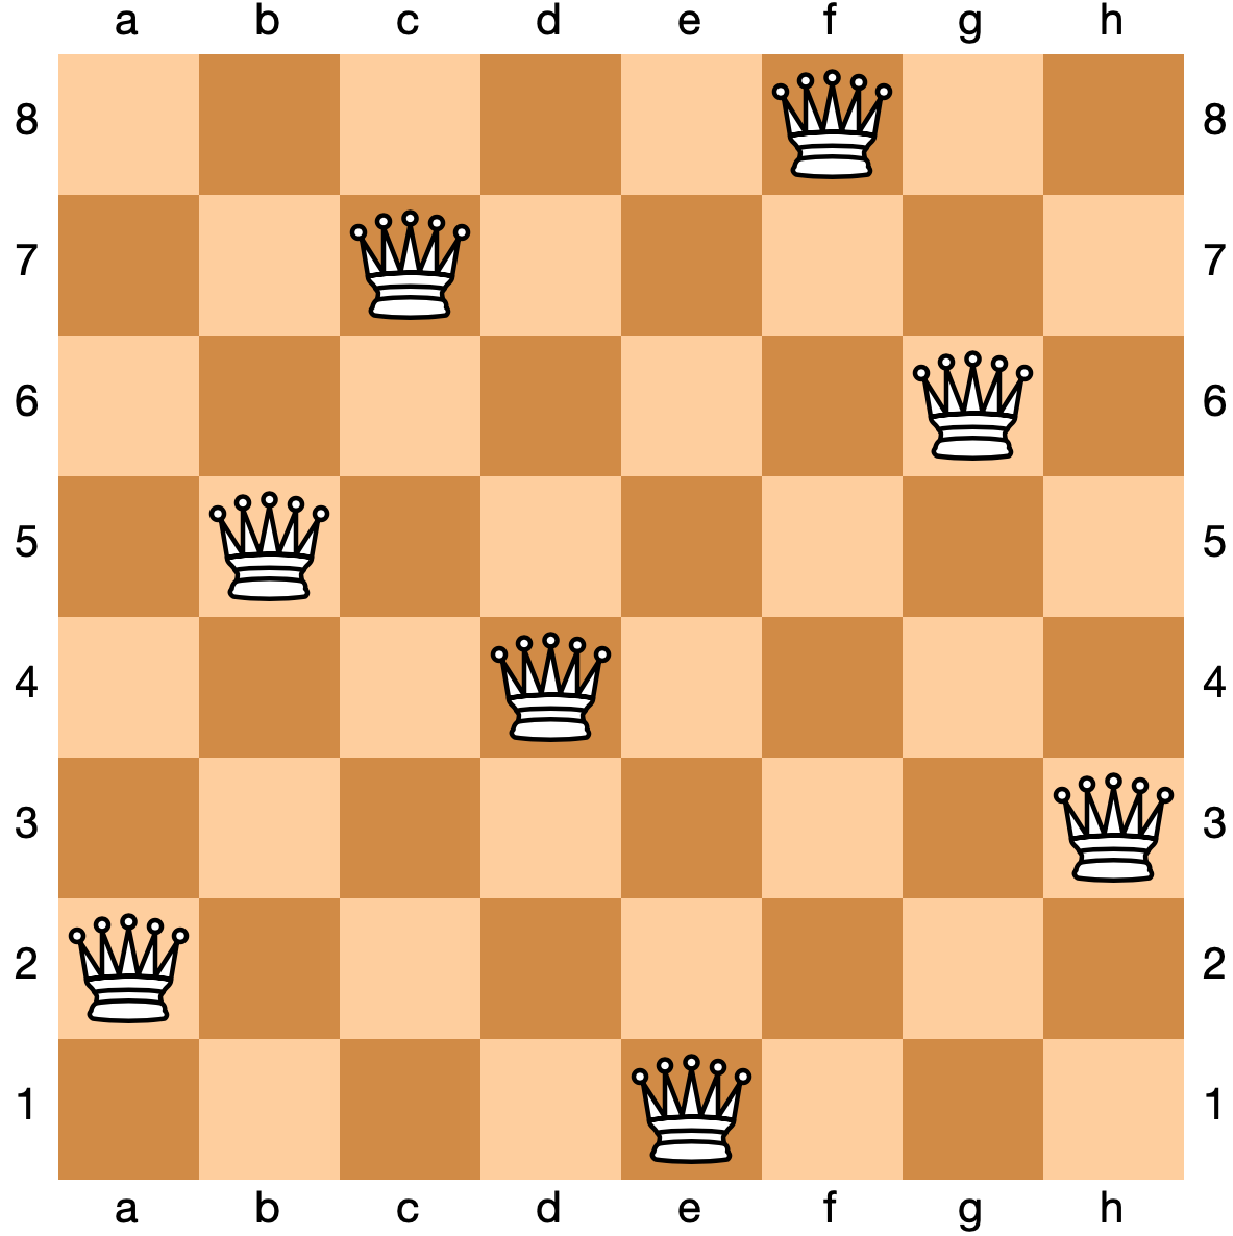
\epsfig{file=Figures/8-queens.pdf, scale=0.8}} 
  \caption{Eine Lösung des 8-Damen-Problems.}
  \label{fig:8-queens.pdf}
\end{figure}

Jessica Roth und Koen Loogman (das sind zwei ehemalige DHBW-Studenten) haben eine Animation des Verfahren von
Davis und Putnam implementiert.  Sie können diese Animation unter der Adresse
\\[0.2cm]
\hspace*{1.3cm}
\href{https://koenloogman.github.io/Animation-Of-N-Queens-Problem-In-JavaScript/}{https://koenloogman.github.io/Animation-Of-N-Queens-Problem-In-JavaScript/}
\\[0.2cm]
im Netz finden und ausprobieren.

Das 8-Damen-Problem ist natürlich nur eine spielerische Anwendung der Aussagen-Logik.
Trotzdem zeigt es die Leistungsfähigkeit des Algorithmus von Davis
und Putnam sehr gut, denn die Menge der Klauseln, die von der Funktion \texttt{allClauses}
berechnet wird, besteht aus 512 verschiedenen Klauseln.  In dieser Klausel-Menge kommen 64 verschiedene
Variablen vor. 

In der Praxis gibt es viele Probleme, die sich in ganz ähnlicher Weise auf die Lösung einer
Menge von Klauseln zurückführen lassen.  Dazu gehört zum Beispiel das Problem, einen
Stundenplan zu erstellen, der gewissen Nebenbedingungen genügt.  Verallgemeinerungen des
Stundenplan-Problems werden in der Literatur als \blue{Scheduling-Probleme} bezeichnet.
Die effiziente Lösung solcher Probleme ist Gegenstand der aktuellen Forschung.

\section{Reflexion}
\begin{enumerate}[(a)]
\item Wie haben wir die Menge der aussagenlogischen Formeln definiert?
\item Wie ist die Semantik der aussagenlogischen Formeln festgelegt worden?
\item Wie können wir aussagenlogische Formeln in \textsl{Python} darstellen?
\item Was ist eine Tautologie?
\item Was ist eine konjunktive Normalform?
\item Wie können Sie die konjunktive Normalform einer gegebenen aussagenlogischen Formel berechnen und wie lässt
      sich diese Berechnung in \textsl{Python} implementieren?
\item Wie haben wir den Beweis-Begriff $M \vdash C$ definiert?
\item Welche Eigenschaften hat der Beweis-Begriff $\vdash$?
\item Wann ist eine Menge von Klauseln lösbar?
\item Wie funktioniert das Verfahren von Davis und Putnam?
\item Wie können Sie das 8-Damen-Problem als aussagenlogisches Problem formulieren?
\end{enumerate}

%\section{Der Kompaktheits-Satz der Aussagen-Logik}
Das Ziel dieses Abschnittes ist der Beweis des Kompaktheits-Satzes der Aussagen-Logik.  
Dieser Satz liegt tiefer als alle bisher behandelten S\"{a}tze.  Wir ben\"{o}tigen den Kompaktheits-Satz
sp\"{a}ter, um die Widerlegungs-Vollst\"{a}ndigkeit der Pr\"{a}dikaten-Logik beweisen zu k\"{o}nnen.
Wir folgen bei unserer Darstellung des Kompaktheits-Satzes dem Artikel von Jon Barwise
\cite{barwise:1991a} aus dem Handbuch der mathematischen Logik \cite{barwise:1991}.

\begin{Definition}[endlich erf\"{u}llbar, maximal endlich erf\"{u}llbar]
  {\em Eine Menge $M$ von aussagenlogischen Formeln hei\3t \emph{endlich erf\"{u}llbar} (abgek\"{u}rzt: e.e.) genau
    dann, wenn jede endliche Teilmenge von $M$ erf\"{u}llbar ist:
    \\[0.2cm]
    \hspace*{1.3cm} 
    $M$ e.e. \quad g.d.w. \quad 
    $\forall E \subseteq M: \textsl{card}(E) < \infty \rightarrow 
    \exists \mathcal{I} \in \textsc{Ali}: \forall f \in E: \mathcal{I}(f) = \mathtt{true}$
    \\[0.2cm]
    Eine Menge $M$ von aussagenlogischen Formeln hei\3t \emph{maximal endlich erf\"{u}llbar}
    (abgek\"{u}rzt m.e.e.) genau dann, wenn $M$ endlich erf\"{u}llbar ist und wenn au\3erdem f\"{u}r
    jede aussagenlogische Formel $f$ entweder $f$ oder die Negation $\neg f$ ein Element von $M$ ist:
    \\[0.2cm]
    \hspace*{1.3cm}
    $M$ m.e.e. \quad g.d.w. \quad 
    $M$ e.e.$\;$ und $\;\forall f \el \mathcal{F}: f \el M \,\vee\, (\neg f) \el M$. \qed
  }
\end{Definition}

\begin{Satz} \label{satz28}
{\em
  Es sei $M$ maximal endlich erf\"{u}llbar.  Dann gilt 
  \\[0.2cm]
  \hspace*{1.3cm}
  $(f \wedge g) \el M$ \quad g.d.w. \quad $f \el M$ und $g \el M$.
}
\end{Satz}

\noindent
\textbf{Beweis}: Wir beweisen beide Richtungen des ``g.d.w.'' getrennt.
\begin{description}
\item[``$\Rightarrow$''] Sei $(f \wedge g) \el M$.  Wir f\"{u}hren den Beweis indirekt und
  nehmen an, es gelte $f \notel M$. Da
  $M$ maximal endlich erf\"{u}llbar ist, muss dann die Formel $\neg f$ ein Element der Menge
  $M$ sein.  Damit enth\"{a}lt $M$ aber die endliche Teilmenge 
  \\[0.2cm]
  \hspace*{1.3cm}
  $E := \{ f \wedge g, \neg f\}$, 
  \\[0.2cm]
  die offenbar nicht erf\"{u}llbar ist, denn jede Belegung, die $f \wedge g$ wahr macht, macht
  sicher auch $f$ wahr und damit $\neg f$ falsch.  Die Unerf\"{u}llbarkeit von $E$ steht im
  Widerspruch zur endlichen Erf\"{u}llbarkeit von $M$.  Damit muss die Annahme $f \notel M$
  falsch sein und wir haben $f \el M$ gezeigt. 

  Der Nachweis von $g \el M$ kann analog gef\"{u}hrt werden.
\item[``$\Leftarrow$''] Sei nun $f \el M$ und $g \el M$.  
  Wir f\"{u}hren den Beweis indirekt und nehmen an, dass $(f \wedge g) \notel M$ gelte.  Da $M$
  maximal endlich erf\"{u}llbar ist, muss dann die Formel $\neg (f \wedge g)$ ein Element der
  Menge $M$ sein.  Dann enth\"{a}lt $M$ aber die endliche Teilmenge
  \\[0.2cm]
  \hspace*{1.3cm}
  $E := \{ \neg (f \wedge g), f, g \}$
  \\[0.2cm]
  die offensichtlich nicht erf\"{u}llbar ist, denn jede Belegung, die $f$ und $g$ wahr macht,
  macht auch die Formel $f \wedge g$ wahr und muss damit die Formel $\neg (f \wedge g)$
  falsch machen.  Die Unerf\"{u}llbarkeit von $E$ steht im Widerspruch zur endlichen
  Erf\"{u}llbarkeit von $M$.  Damit muss die Annahme $(f \wedge g) \notel M$ falsch sein und
  es gilt $(f \wedge g) \el M$. \qed
\end{description}

\begin{Satz} \label{satz29}
{\em
  Es sei $M$ maximal endlich erf\"{u}llbar. Dann gilt:
  \begin{enumerate}
  \item $(\neg f) \el M$ \quad g.d.w. $f \notel M$.
  \item $(f \vee g) \el M$ \quad g.d.w. $f \el M$ oder $g \el M$.
  \item $(f \rightarrow g) \el M$ \quad g.d.w. $(\neg f) \el M$ oder $g \el M$.
  \item $(f \leftrightarrow g) \el M$ \quad g.d.w. 
        $(f \rightarrow g) \el M$ und $(g \rightarrow f) \el M$.
  \end{enumerate}
}
\end{Satz}

\noindent
\textbf{Beweis}:  Der Beweis der einzelnen Behauptungen verl\"{a}uft ganz analog zu dem Beweis
von Satz \ref{satz28}.  Exemplarisch zeigen wir den Beweis der vierten Behauptung.
Wir beweisen beide  Richtungen des ``g.d.w.'' getrennt.
\begin{description}
\item[``$\Rightarrow$''] Sei $(f \leftrightarrow g) \el M$.  Wir f\"{u}hren den Beweis indirekt und
  nehmen an, es gelte $(f \rightarrow g) \notel M$. Da
  $M$ maximal endlich erf\"{u}llbar ist, muss dann die Formel $\neg (f \rightarrow g)$ ein Element der Menge
  $M$ sein.  Damit enth\"{a}lt $M$ aber die endliche Teilmenge 
  \\[0.2cm]
  \hspace*{1.3cm}
  $E := \{ f \leftrightarrow g, \neg (f \rightarrow g)\}$, 
  \\[0.2cm]
  die offenbar nicht erf\"{u}llbar ist, denn jede Belegung, die $f \leftrightarrow g$ wahr macht, macht
  sicher auch $f \rightarrow g$ wahr und damit $\neg (f \rightarrow g)$ falsch.  Die
  Unerf\"{u}llbarkeit von $E$ steht im 
  Widerspruch zur endlichen Erf\"{u}llbarkeit von $M$.  Damit muss die Annahme $(f \rightarrow g) \notel M$
  falsch sein und wir haben $(f \rightarrow g) \el M$ gezeigt. 

  Der Nachweis von $(g \rightarrow f) \el M$ kann analog gef\"{u}hrt werden.
\item[``$\Leftarrow$''] Sei nun $(f \rightarrow g) \el M$ und $(g \rightarrow f) \el M$.  
  Wir f\"{u}hren den Beweis indirekt und nehmen an, dass $(f \leftrightarrow g) \notel M$ gelte.  Da $M$
  maximal endlich erf\"{u}llbar ist, muss dann die Formel $\neg (f \leftrightarrow g)$ ein Element der
  Menge $M$ sein.  Dann enth\"{a}lt $M$ aber die endliche Teilmenge
  \\[0.2cm]
  \hspace*{1.3cm}
  $E := \{ \neg (f \leftrightarrow g), f \rightarrow g, g \rightarrow f \}$
  \\[0.2cm]
  die offensichtlich nicht erf\"{u}llbar ist, denn jede Belegung, die $f \rightarrow g$ und $g
  \rightarrow f$ wahr macht,
  macht auch die Formel $f \leftrightarrow g$ wahr und muss damit die Formel $\neg (f \leftrightarrow g)$
  falsch machen.  Die Unerf\"{u}llbarkeit von $E$ steht im Widerspruch zur endlichen
  Erf\"{u}llbarkeit von $M$.  Damit muss die Annahme $(f \leftrightarrow g) \notel M$ falsch sein und
  es gilt $(f \leftrightarrow g) \el M$. \qed
\end{description}

\begin{Satz} \label{satz30}
{\em
  Jede maximal endlich erf\"{u}llbare Menge $M$ ist erf\"{u}llbar.
}
\end{Satz}

\noindent
\textbf{Beweis}:
Die Menge $M$ sei maximal endlich erf\"{u}llbar.  Wir konstruieren eine Variablen-Belegung
$\mathcal{I}$ wie folgt:
\\[0.2cm]
\hspace*{1.3cm}
$\mathcal{I} := \bigl\{ \pair(p, \mathtt{true})  \mid p \el M \bigr\} \cup
                \bigl\{ \pair(p, \mathtt{false}) \mid p \notel M \bigr\}$.
\\[0.2cm]
Wir behaupten, dass diese Belegung  jede Formel $f\el M$ wahr und jede Formel $f \notel M$
falsch macht und beweisen diese
Behauptung durch Induktion nach dem Aufbau der Formel $f$. Wir beweisen also
\\[-0.2cm]
\hspace*{1.3cm}
$f \el M$ \quad g.d.w. \quad $\mathcal{I}(f) = \mathtt{true}$
\\[0.2cm]
durch Induktion nach $f$.
\begin{enumerate}
\item $f = p \el \mathcal{P}$, \ $f$ ist also eine aussagenlogische Variable.
    
      Falls $p \el M$ ist, dann folgt $\mathcal{I}(f) = \mathtt{true}$ aus der Definition
      von $\mathcal{I}$.   Falls $p \notel M$ ist, folgt aus der Definition von
      $\mathcal{I}$ sofort $\mathcal{I}(p) = \mathtt{false}$.
      
\item $f = \neg g$.  

      Sei zun\"{a}chst $f \el M$. Nach Satz \ref{satz29} folgt aus $(\neg g) \el M$ sofort
      $g \notel M$.  Nach Induktions-Voraussetzung gilt dann $\textsl{I}(g) = \mathtt{false}$ und
      daraus folgt sofort $\textsl{I}(f) = \textsl{I}(\neg g) = \mathtt{true}$.
      
      Sei nun $f \notel M$. Wieder nach Satz \ref{satz29} folgt aus $(\neg g) \notel M$ sofort
      $g \el M$.  Nach Induktions-Voraussetzung gilt dann $\textsl{I}(g) = \mathtt{true}$ und
      daraus folgt sofort $\textsl{I}(f) = \textsl{I}(\neg g) = \mathtt{false}$.
\item $f = (g \wedge h)$.

      Sei zun\"{a}chst $f \el M$.  Nach Satz \ref{satz29} folgt aus $(g \wedge h) \el M$ sofort
      $g \el M$ und $h \el M$.  Wenden wir die Induktions-Voraussetzung auf $g$ und $h$ an, so sehen
      wir, dass $\textsl{I}(g) = \mathtt{true}$ und
      $\textsl{I}(h) = \mathtt{true}$ gelten muss, woraus sofort
      $\textsl{I}(f) = \textsl{I}(g \wedge h) = \mathtt{true}$ folgt.
      
      Sei nun $f \notel M$. Nach Satz \ref{satz29} folgt aus $(g \wedge h) \notel M$, dass
      entweder $g \notel M$ oder $h \notel M$ ist.  Wir betrachten nur den Fall $g \notel M$, 
      der Fall $h \notel M$ ist analog.  Aus $g \notel M$ folgt mit der Induktions-Voraussetzung,
      dass $\mathcal{I}(g) = \mathtt{false}$ gilt.  Dass impliziert aber die Behauptung 
      $\textsl{I}(g \wedge h) = \mathtt{false}$, womit wir $\mathcal{I}(f) = \mathtt{false}$ haben.
\item $f = (g \vee h)$,
      $f = (g \rightarrow h)$,
      $f = (g \leftrightarrow h)$.
      
      Da der Beweis dieser F\"{a}lle ganz analog zum Beweis des Falles $f = (f \wedge g)$ verl\"{a}uft,
      k\"{o}nnen wir auf einen expliziten Beweis dieser F\"{a}lle verzichten. \qed
\end{enumerate}

\begin{Satz}[Kompaktheits-Satz]
{\em
  Die Menge $M$ sei endlich erf\"{u}llbar.  Dann ist $M$ erf\"{u}llbar, es gibt also eine aussagenlogische
  Belegung $\mathcal{I}$, so dass gilt:
  \\[0.2cm]
  \hspace*{1.3cm}
  $\forall f \in M: \mathcal{I}(f) = \mathtt{true}$.
} 
\end{Satz}

\noindent
\textbf{Beweis}:  Wir werden $M$ so zu einer maximal endlich erf\"{u}llbaren Menge $\widehat{M}$
erweitern, dass 
\\[0.2cm]
\hspace*{1.3cm}
$M \subseteq \widehat{M}$
\\[0.2cm]
gilt.  Da die Menge $\widehat{M}$ nach Satz \ref{satz30} erf\"{u}llbar ist, ist $M$ als Teilmenge von
$\widehat{M}$ dann erst recht erf\"{u}llbar.
Zu diesem Zweck definieren wir eine Folge $(M_n)_{n\in \mathbb{N}}$ von Mengen, die alle endlich
erf\"{u}llbar sind und die in einem gewissen Sinne gegen die Menge $\widehat{M}$ konvergieren.
Die Definition der Mengen $M_n$ verl\"{a}uft durch Induktion nach der Zahl $n$.  Bevor wir diese
Induktion durchf\"{u}hren k\"{o}nnen, ben\"{o}tigen wir eine \emph{Aufz\"{a}hlung} aller aussagenlogischen Formeln.
Darunter verstehen wir eine Folge aussagenlogischer Formeln $(g_n)_{n \in \mathbb{N}}$, in der jede
aussagenlogische Formel mindestens einmal vorkommt, es soll also gelten:
\\[0.2cm]
\hspace*{1.3cm}
$\forall f \in \mathcal{F}: \exists n \in \mathbb{N}: f = g_n$.
\\[0.2cm]
Falls die Menge der Aussagen-Variablen endlich ist, so kann eine solche Folge zum Beispiel dadurch konstruiert
werden, dass wir erst alle Formeln der L\"{a}nge 1, dann die Formeln der L\"{a}nge 2 und so weiter
aufz\"{a}hlen.  

Die induktive Definition der Mengen $M_n$ verl\"{a}uft nun wie folgt.
\begin{enumerate}
\item[I.A.] $n = 0$:  Wir setzen
  \\[0.2cm]
  \hspace*{1.3cm}
  $M_0 := M$.
  \\[0.2cm]
  Dann ist die Menge $M_0$ nach Voraussetzung endlich erf\"{u}llbar.
\item[I.S.] $n \mapsto n + 1$:  Die Definition von $M_{n+1}$ erfolgt \"{u}ber eine Fall-Unterscheidung:
  \\[0.2cm]
  \hspace*{1.3cm}
  $M_{n+1} := \left\{
  \begin{array}[c]{ll}
    M_n \cup \{ f_n \}      & \mbox{falls $M_n \cup \{ f_n \}$ endlich erf\"{u}llbar ist;} \\[0.2cm]
    M_n \cup \{ \neg f_n \} & \mbox{sonst.}
  \end{array}
  \right.
  $
  \\[0.2cm]
  Wir m\"{u}ssen zeigen, dass $M_{n+1}$ endlich erf\"{u}llbar ist.  Es gibt zwei F\"{a}lle.
  \begin{enumerate}
  \item $M_n \cup \{ f_n \}$ ist endlich erf\"{u}llbar.

        Dann gilt $M_{n+1} = M_n \cup \{ f_n \}$ und die Behauptung ist trivial.
  \item $M_n \cup \{ f_n \}$ ist nicht endlich erf\"{u}llbar.

        Da $M_n$ alleine nach Induktions-Voraussetzung endlich erf\"{u}llbar ist, muss es dann eine
        endliche Teilmenge $E = \{ e_1, \cdots, e_k \} \subseteq M_n$ geben, so dass
        \\[0.2cm]
        \hspace*{1.3cm}
        $E \cup \{ f_n \}$
        \\[0.2cm]
        nicht erf\"{u}llbar ist.  Damit gilt dann
        \\[0.2cm]
        \hspace*{1.3cm}
        $\{ e_1, \cdots, e_m, f_n \} \models \falsum$
        \\[0.2cm]
        und daraus folgt
        \\[0.2cm]
        \hspace*{1.3cm}
        $ \models e_1 \wedge \cdots \wedge e_n \rightarrow \neg f_n$.
        \\[0.2cm]
        Wir f\"{u}hren den Beweis nun indirekt und nehmen an, dass die Menge
        \\[0.2cm]
        \hspace*{1.3cm}
        $M_n \cup \{ \neg f_n \}$ 
        \\[0.2cm]
        nicht endlich erf\"{u}llbar w\"{a}re.  Dann gibt es eine endliche Menge 
        $G = \{ g_1, \cdots, g_k \} \subseteq M_n$,
        so dass gilt:
        \\[0.2cm]
        \hspace*{1.3cm}
        $\{ g_1, \cdots, g_k, \neg f_n \} \models \falsum$.
        \\[0.2cm]
        Daraus folgt aber
        \\[0.2cm]
        \hspace*{1.3cm}
        $\models g_1 \wedge \cdots \wedge g_k \rightarrow f_n$.
        \\[0.2cm]
        Insgesamt haben wir damit aber sowohl
        \\[0.2cm]
        \hspace*{1.3cm}
        $\models e_1 \wedge \cdots \wedge e_m \wedge g_1 \wedge \cdots \wedge g_k \rightarrow f_n$
        \\
        als auch 
        \\[-0.2cm]
        \hspace*{1.3cm}
        $\models e_1 \wedge \cdots \wedge e_m \wedge g_1 \wedge \cdots \wedge g_k \rightarrow \neg f_n$.
        \\[0.2cm]
        Zusammengenommen zeigt dies, dass die Menge $G := \{ e_1, \cdots, e_m, g_1, \cdots, g_k \}$
        nicht erf\"{u}llbar ist:
        \\[0.2cm]
        \hspace*{1.3cm}
        $\{ e_1, \cdots, e_m, g_1, \cdots, g_k \} \models \falsum$.
        \\[0.2cm]
        Dies steht im Widerspruch dazu, dass diese Menge eine endliche Teilmenge von $M_n$ ist und
        $M_n$ ist nach Induktions-Voraussetzung endlich erf\"{u}llbar.  Daher haben wir die Annahme,
        dass $M_n \cup \{ \neg f_n \}$ nicht endlich erf\"{u}llbar ist, widerlegt. 
  \end{enumerate}
  Nach Konstruktion der Mengen $M_n$ gilt offenbar
  \\[0.2cm]
  \hspace*{1.3cm}
  $M_0 \subseteq M_1 \subseteq M_2 \subseteq \cdots \subseteq M_n \subseteq M_{n+1} \subseteq \cdots$.
  \\[0.2cm]
  Daher definieren wir die Menge $\widehat{M}$ nun als den Grenzwert der Folge $(M_n)_{n \in \mathbb{N}}$:
  \\[0.2cm]
  \hspace*{1.3cm}
  $\widehat{M} = \bigcup\limits_{n \in \mathbb{N}} M_n$.
  \\[0.2cm]
  Wir zeigen zun\"{a}chst, dass $\widehat{M}$ endlich erf\"{u}llbar ist.  Sei also $E$ eine endliche
  Teilmenge von $\widehat{M}$:
  \\[0.2cm]
  \hspace*{1.3cm}
  $E = \{ e_1, \cdots, e_m \} \subseteq \bigcup\limits_{n \in \mathbb{N}} M_n$.
  \\[0.2cm]
  Dann gibt es f\"{u}r jedes $i \in \{ 1, \cdots, m \}$ eine Zahl $n(i)$, so dass
  \\[0.2cm]
  \hspace*{1.3cm}
  $e_i \in M_{n(i)}$ 
  \\[0.2cm]
  ist.  Wir definieren
  \\[0.2cm]
  \hspace*{1.3cm}
  $\widehat{n} := \max\bigl(\bigl\{n(1), \cdots, n(m) \bigr\}\bigr)$
  \\[0.2cm]
  Daraus folgt aber sofort $E \subseteq M_{\widehat{n}}$ und da $M_{\widehat{n}}$ endlich erf\"{u}llbar
  ist, muss die Menge $E$ als endliche Teilmenge von $M_{\widehat{n}}$ erf\"{u}llbar sein.
  Damit haben wir gezeigt, dass $\widehat{M}$ endlich erf\"{u}llbar ist.

  Als n\"{a}chstes zeigen wir, dass $\widehat{M}$ maximal endlich erf\"{u}llbar ist.  Betrachten wir eine
  beliebige aussagenlogische Formel $f$.  Wir m\"{u}ssen zeigen, dass entweder $f \el \widehat{M}$ oder 
  $(\neg f) \el \widehat{M}$ gilt.  Wir hatten vorausgesetzt, dass die Folge $(f_n)_{n \in \mathbb{N}}$ 
  die Menge aller aussagenlogischen Formeln aufz\"{a}hlt.  Also gibt es ein $n$, so dass $f = f_n$ ist.
  Nach Definition gilt dann aber 
  \\[0.2cm]
  \hspace*{1.3cm}
  $M_{n+1} = M_n \cup \{ f_n \}$ \quad oder \quad 
  $M_{n+1} = M_n \cup \{ \neg f_n \}$
  \\[0.2cm]
  und da $M_{n+1} \subseteq \widehat{M}$ ist, folgt
  \\[0.2cm]
  \hspace*{1.3cm}
  $f_n \el \widehat{M}$ \quad oder \quad
  $(\neg f_n) \el \widehat{M}$.
  \\[0.2cm]
  Also ist $\widehat{M}$ maximal endlich erf\"{u}llbar und daher ist $\widehat{M}$ nach Satz \ref{satz30} erf\"{u}llbar. \qed
\end{enumerate}

%%% Local Variables: 
%%% mode: latex
%%% TeX-master: "logik"
%%% End: 


%%% Local Variables: 
%%% mode: latex
%%% TeX-master: "logic"
%%% ispell-local-dictionary: "deutsch8"
%%% End: 

\chapter{Prädikatenlogik}
In der \blue{Aussagenlogik} haben wir die Verknüpfung von elementaren Aussagen mit \blue{Junktoren} untersucht.
Die \blue{Prädikatenlogik} untersucht zusätzlich auch die Struktur dieser elementaren Aussagen.  Dazu werden in der
Prädikatenlogik die folgenden zusätzlichen Begriffe eingeführt:
\begin{enumerate}
\item Als Bezeichnungen für Objekte werden \blue{Terme} verwendet.
\item Diese Terme werden aus \blue{Objekt-Variablen} und \blue{Funktions-Zeichen}
      zusammengesetzt.  In den folgenden Beispielen ist $x$ eine Objekt-Variable, während
      \textsl{vater} und \textsl{mutter} einstellige Funktions-Zeichen sind. \textsl{issac} ist ein
      nullstelliges Funktions-Zeichen:
      \\[0.2cm]
      \hspace*{1.3cm}
      $\textsl{vater}(x),\quad \textsl{mutter}(\textsl{isaac})$.
      \\[0.2cm]
      Nullstellige Funktions-Zeichen werden im Folgenden auch als \blue{Konstanten} bezeichnet und an Stelle
      von Objekt-Variablen reden wir kürzer nur von Variablen.
\item Verschiedene Objekte werden durch \blue{Prädikats-Zeichen} in Relation gesetzt.  In den folgenden
      Beispielen benutzen wir die Prädikats-Zeichen \textsl{istBruder} und $<$:
      \\[0.2cm]
      \hspace*{1.3cm}
      $\textsl{istBruder}\bigl(\textsl{albert}, \textsl{vater}(\textsl{bruno})\bigr),\quad x+7 < x\cdot 7$.
      \\[0.2cm]
      Die dabei entstehenden Formeln werden als \blue{atomare} Formeln bezeichnet.
\item Atomare Formeln lassen sich durch aussagenlogische Junktoren verknüpfen:
      \\[0.2cm]
      \hspace*{1.3cm}
      $x > 1 \rightarrow x + 7 < x \cdot  7$.
\item Schließlich werden \blue{Quantoren} eingeführt, um zwischen \blue{existentiell} und
      \blue{universell} quantifizierten Variablen unterscheiden
      zu können:
      \\[0.2cm]
      \hspace*{1.3cm}
      $\forall x \in \mathbb{R}: \exists n \in \mathbb{N}: x < n$.
\end{enumerate}
Wir werden im nächsten Abschnitt die \href{https://de.wikipedia.org/wiki/Syntax}{Syntax} der
prädikatenlogischen Formeln festlegen, wir werden also festlegen, welche Strings wir als aussagenlogische
Formeln zulassen.  Im darauf folgenden Abschnitt beschäftigen wir uns mit der 
\href{https://de.wikipedia.org/wiki/Semantik}{Semantik} dieser Formeln, dort spezifizieren wir also die
Bedeutung der Formeln.

\section{Syntax der Prädikatenlogik}
Zunächst definieren wir den Begriff der \blue{Signatur}.  Inhaltlich ist das nichts anderes als eine 
strukturierte Zusammenfassung von Variablen, Funktions- und Prädikats-Zeichen zusammen mit
einer Spezifikation der Stelligkeit dieser Zeichen.
 
\begin{Definition}[Signatur]
  Eine \blue{Signatur} ist ein 4-Tupel \\[0.2cm]
  \hspace*{1.3cm} $\Sigma = \langle \mathcal{V}, \mathcal{F}, \mathcal{P}, \textsl{arity} \rangle$, \\[0.2cm]
  für das Folgendes gilt: 
  \begin{enumerate}
  \item $\mathcal{V}$ ist die Menge der \blue{Variablen}.
  \item $\mathcal{F}$ ist die Menge der \blue{Funktions-Zeichen}.
  \item $\mathcal{P}$ ist die Menge der \blue{Prädikats-Zeichen}.
  \item $\textsl{arity}$ ist eine Funktion, die jedem Funktions- und jedem Prädikats-Zeichen seine
        \blue{Stelligkeit} zuordnet: \\[0.2cm]
        \hspace*{1.3cm} $\textsl{arity}: \mathcal{F} \cup \mathcal{P} \rightarrow \mathbb{N}$. \\[0.2cm]
        Wir sagen, dass das Funktions- oder Prädikats-Zeichen $f$ ein
        $n$-stelliges Zeichen ist, falls $\textsl{arity}(f) = n$ gilt.
  \item Da wir in der Lage sein müssen, Variablen, Funktions- und Prädikats-Zeichen
        unterscheiden zu können, vereinbaren wir, dass die Mengen $\mathcal{V}$,
        $\mathcal{F}$ und $\mathcal{P}$ paarweise disjunkt sein müssen: \\[0.2cm] 
        \hspace*{1.3cm} $\mathcal{V} \cap \mathcal{F} = \{\}$, \quad
                        $\mathcal{V} \cap \mathcal{P} = \{\}$, \quad und \quad
                        $\mathcal{F} \cap \mathcal{P} = \{\}$. \eox
  \end{enumerate}
\end{Definition}

\noindent
Als Bezeichner für Objekte verwenden wir Ausdrücke, die aus Variablen und
Funktions-Zeichen aufgebaut sind.  Solche Ausdrücke nennen wir \blue{Terme}.  

\begin{Definition}[Terme,  $\mathcal{T}_\Sigma$]
  Ist $\Sigma = \langle \mathcal{V}, \mathcal{F}, \mathcal{P}, \textsl{arity} \rangle$ eine Signatur, so definieren wir die Menge der \blue{$\Sigma$-Terme}
  \blue{$\mathcal{T}_\Sigma$} induktiv:
  \begin{enumerate}
  \item Für jede Variable $x \in \mathcal{V}$ gilt $x \in \mathcal{T}_\Sigma$.  Jede Variable ist also auch
        ein Term.
  \item Ist $f \in \mathcal{F}$ ein n-stelliges Funktions-Zeichen und sind 
        $t_1,\cdots,t_n \el \mathcal{T}_\Sigma$, so gilt 
        \\[0.2cm]
        \hspace*{1.3cm} $f(t_1,\cdots,t_n) \el \mathcal{T}_\Sigma$,
        \\[0.2cm]
        der Ausdruck  $f(t_1,\cdots,t_n) \el \mathcal{T}_\Sigma$ ist also ein Term.
        Falls $c \in \mathcal{F}$ ein 0-stelliges Funktions-Zeichen ist, lassen wir auch die Schreibweise
        $c$ anstelle von $c()$ zu.  In diesem Fall nennen wir $c$ eine \blue{Konstante}.
        \eox
  \end{enumerate}
\end{Definition}

\example
Es sei 
\begin{enumerate}
\item $\mathcal{V} := \{ x, y, z \}$ die Menge der Variablen,
\item $\mathcal{F} := \{ 0, 1, \mathtt{+}, \mathtt{-}, * \}$ die Menge der Funktions-Zeichen,
\item $\mathcal{P} := \{\mathtt{=}, \leq\}$ die Menge der Prädikats-Zeichen,
\item $\textsl{arity} := \bigl\{ \pair(0,0), \pair(1,0), \pair(\mathtt{+},2), \pair(\mathtt{-},2),
  \pair(*,2), \pair(=,2), \pair(\leq,2) \bigr\}$, \\[0.2cm]
      gibt die Stelligkeit der Funktions- und Prädikats-Zeichen an und
\item $\Sigma_\mathrm{arith} := \langle \mathcal{V}, \mathcal{F}, \mathcal{P}, \textsl{arity} \rangle$
      sei eine Signatur.
\end{enumerate}
Dann können wir wie folgt $\Sigma_{\mathrm{arith}}$-Terme konstruieren:
\begin{enumerate}
\item $x, y, z \in \mathcal{T}_{\Sigma_{\mathrm{arith}}}$, \\[0.2cm]
      denn alle Variablen sind auch $\Sigma_{\mathrm{arith}}$-Terme.
\item $0, 1 \in \mathcal{T}_{\Sigma_{\mathrm{arith}}}$,  \\[0.2cm]
      denn $0$ und $1$ sind $0$-stellige Funktions-Zeichen.
\item $\mathtt{+}(0,x) \in \mathcal{T}_{\Sigma_{\mathrm{arith}}}$, \\[0.2cm]
      denn es gilt $0 \in \mathcal{T}_{\Sigma_{\mathrm{arith}}}$, $x \in \mathcal{T}_{\Sigma_{\mathrm{arith}}}$ und 
      $\mathtt{+}$ ist ein 2-stelliges Funktions-Zeichen.
\item $*(\mathtt{+}(0,x),1) \in \mathcal{T}_{\Sigma_{\mathrm{arith}}}$, \\[0.2cm]
      denn $\mathtt{+}(0,x) \in \mathcal{T}_{\Sigma_{\mathrm{arith}}}$, $1 \in \mathcal{T}_{\Sigma_{\mathrm{arith}}}$ und
      $*$ ist ein 2-stelliges Funktions-Zeichen.
\end{enumerate}
In der Praxis werden wir für bestimmte zweistellige Funktionen eine Infix-Schreibweise
verwenden.  Diese ist dann als Abkürzung für die oben definierte Darstellung zu verstehen.
\eox


Als nächstes definieren wir den Begriff der \blue{atomaren Formeln}.  Darunter verstehen wir
solche Formeln, die man nicht in kleinere Formeln zerlegen kann: Atomare Formeln enthalten also
weder Junktoren noch Quantoren. 
\begin{Definition}[Atomare Formeln,  $\mathcal{A}_\Sigma$]
  Gegeben sei eine Signatur $\Sigma = \langle \mathcal{V}, \mathcal{F}, \mathcal{P}, \textsl{arity} \rangle$. 
  Die Menge der atomaren $\Sigma$-Formeln $\mathcal{A}_\Sigma$
  wird wie folgt definiert:  Ist $p \el \mathcal{P}$ ein $n$-stelliges Prädikats-Zeichen
  und sind $n$ $\Sigma$-Terme $t_1$, $\cdots$, $t_n$ gegeben, so ist
  $p(t_1,\cdots,t_n)$ eine \blue{atomaren $\Sigma$-Formel}: \\[0.2cm]
  \hspace*{1.3cm} $p(t_1,\cdots,t_n) \in \mathcal{A}_\Sigma$.  \\[0.2cm]
  Falls $p$ ein 0-stelliges Prädikats-Zeichen ist, dann schreiben wir auch $p$ anstelle von $p()$.
  In diesem Fall nennen wir $p$ eine \blue{Aussage-Variable}.
  \eox
\end{Definition}

\example
Setzen wir das letzte Beispiel fort, so können wir sehen, dass \\[0.2cm]
\hspace*{1.3cm} $\mathtt{=}(*(\mathtt{+}(0,x),1),0)$ \\[0.2cm]
eine atomare $\Sigma_\mathrm{arith}$-Formel ist.  Beachten Sie, dass wir bisher noch nichts über den Wahrheitswert von solchen 
Formeln ausgesagt haben.  Die Frage, wann eine Formel als wahr oder falsch gelten soll,
wird erst im nächsten Abschnitt untersucht.
\eox


Bei der Definition der prädikatenlogischen Formeln ist es notwendig,
zwischen sogenannten \blue{gebundenen} und \blue{freien} Variablen zu unterscheiden.
Wir führen diese Begriffe zunächst informal mit Hilfe eines Beispiels aus der Analysis ein.
Wir betrachten die folgende Gleichung: \\[0.2cm]
\hspace*{1.3cm}
 $\ds\int_{0}^{x} y \cdot  t\, d t = \frac{1}{2} \cdot x^2 \cdot  y$ 
\\[0.2cm]
In dieser Gleichung treten die Variablen $x$ und $y$ \blue{frei} auf, während die Variable $t$ durch das Integral
\blue{gebunden} wird.  Damit meinen wir folgendes: Wir können in dieser Gleichung für $x$ und $y$ beliebige Werte
 einsetzen, ohne dass sich an der 
Gültigkeit der Formel etwas ändert.  Setzen wir zum Beispiel für $x$ den Wert $2$ ein, so erhalten wir \\[0.2cm]
\hspace*{1.3cm}
$\ds\int_{0}^{2} y \cdot  t\, d t = \frac{1}{2} \cdot 2^2 \cdot  y$ \\[0.2cm]
und diese Gleichung ist ebenfalls gültig.  Demgegenüber macht es keinen Sinn, wenn wir für die gebundene Variable
 $t$ eine Zahl einsetzen würden.
Die linke Seite der entstehenden Gleichung wäre einfach undefiniert.  Wir können für $t$
höchstens eine andere Variable einsetzen. 
Ersetzen wir die Variable $t$ beispielsweise durch $u$, so erhalten wir \\[0.2cm]
\hspace*{1.3cm}
$\ds\int_{0}^{x} y \cdot  u\, d u = \frac{1}{2} \cdot x^2 \cdot  y$ 
\\[0.2cm]
und das ist inhaltlich dieselbe Aussage wie oben.  Das funktioniert allerdings nicht mit jeder Variablen. Setzen wir
für $t$ die Variable $y$ ein, so erhalten wir \\[0.2cm]
\hspace*{1.3cm}
$\ds\int_{0}^{x} y \cdot  y\, d y = \frac{1}{2} \cdot x^2 \cdot  y$. \\[0.2cm]
Diese Aussage ist aber falsch!  Das Problem liegt darin, dass bei der Ersetzung von $t$ durch $y$ die vorher freie Variable
$y$ gebunden wurde.  

Ein ähnliches Problem erhalten wir, wenn wir für $y$ beliebige Terme einsetzen.  Solange diese Terme die Variable $t$ 
nicht enthalten, geht alles gut.  Setzen wir beispielsweise für $y$  den Term $x^2$ ein, so erhalten
wir \\[0.2cm]
\hspace*{1.3cm}
$\ds\int_{0}^{x} x^2 \cdot  t\, d t = \frac{1}{2} \cdot x^2 \cdot  x^2$ 
\\[0.2cm]
und diese Formel ist gültig.  Setzen wir allerdings für $y$ den Term $t^2$ ein, so erhalten wir \\[0.2cm]
\hspace*{1.3cm}
$\ds\int_{0}^{x} t^2 \cdot  t\, d t = \frac{1}{2} \cdot x^2 \cdot  t^2$ 
\\[0.2cm]
und diese Formel ist nicht mehr gültig. 

In der Prädikatenlogik binden die Quantoren ``$\forall$'' (\blue{für alle}) und ``$\exists$''
(\blue{es gibt}) Variablen in ähnlicher Weise,  wie der Integral-Operator ``$\int \cdot\; \mathtt{d}t$'' in
der Analysis Variablen bindet.  Die oben gemachten Ausführungen zeigen, dass es zwei verschiedene Arten von 
Variable gibt: \blue{freie Variablen} und \blue{gebundene Variablen}.
Um diese Begriffe präzisieren zu können, definieren wir zunächst für einen
$\Sigma$-Term $t$ die Menge der in $t$ enthaltenen Variablen.

\begin{Definition}[$\var(t)$]
  Ist $\Sigma = \langle \mathcal{V}, \mathcal{F}, \mathcal{P}, \textsl{arity} \rangle$ eine Signatur und ist
  $t$ ein $\Sigma$-Term, so definieren wir die Menge \blue{$\var(t)$} der Variablen, die in $t$
    auftreten, durch Induktion nach dem Aufbau des Terms:
    \begin{enumerate}
    \item $\var(x) := \{ x \}$ \quad für alle $x \in \mathcal{V}$,
    \item $\var\bigl(f(t_1,\cdots,t_n)\bigr) := \var(t_1) \cup \cdots \cup \var(t_n)$.
          \eox
    \end{enumerate}
\end{Definition}


\begin{Definition}[$\Sigma$-Formel,  $\mathbb{F}_\Sigma$, gebundene und freie Variablen, $\textsl{BV}(F)$,  $\textsl{FV}(F)$] 
\label{praedikaten-formel} \hspace*{\fill} \\
    Es sei $\Sigma = \langle \mathcal{V}, \mathcal{F}, \mathcal{P}, \textsl{arity} \rangle$ eine Signatur.
    Die Menge der {\color{blue}$\Sigma$-\emph{Formeln}} bezeichnen wir mit $\mathbb{F}_\Sigma$.
    Wir definieren diese Menge induktiv.
    Gleichzeitig definieren wir für jede Formel $F\el \mathbb{F}_\Sigma$ die Menge $\textsl{BV}(F)$ der in $F$ 
    \blue{gebunden} auftretenden Variablen und die Menge $\textsl{FV}(F)$ der in $F$ \blue{frei} auftretenden Variablen.
    \begin{enumerate}
    \item Es gilt $\falsum \in \mathbb{F}_\Sigma$ und $\verum \in \mathbb{F}_\Sigma$ und wir definieren \\[0.2cm]
          \hspace*{1.3cm} $\FV(\falsum) := \FV(\verum) := \BV(\falsum) := \BV(\verum) := \{\}$.
    \item Ist $F = p(t_1,\cdots,t_n)$ eine atomare $\Sigma$-Formel, so gilt $F \in \mathbb{F}_\Sigma$.  Weiter definieren wir:
          \begin{enumerate}
          \item $\FV\bigl(p(t_1,\cdots,t_n) \bigr) := \var(t_1) \cup \cdots \cup \var(t_n)$.
          \item $\BV\bigl(p(t_1,\cdots,t_n) \bigr) := \{\}$.
          \end{enumerate}
    \item Ist $F \in \mathbb{F}_\Sigma$, so gilt $\neg F \in \mathbb{F}_\Sigma$. Weiter definieren wir:
          \begin{enumerate}
          \item $\FV\bigl( \neg F \bigr) := \FV(F)$.
          \item $\BV\bigl( \neg F \bigr) := \BV(F)$.
          \end{enumerate}
    \item Sind $F, G \in \mathbb{F}_\Sigma$ und gilt außerdem \\[0.2cm]
          \hspace*{1.3cm}
          $\bigl(\FV(F) \cup \FV(G)\bigr) \cap \bigl(\BV(F) \cup \BV(G)) = \{\}$,
          \\[0.2cm]
          so gilt auch
          \begin{enumerate}
          \item $(F \wedge G) \in \mathbb{F}_\Sigma$,
          \item $(F \vee G) \in \mathbb{F}_\Sigma$,
          \item $(F \rightarrow G) \in \mathbb{F}_\Sigma$,
          \item $(F \leftrightarrow G) \in \mathbb{F}_\Sigma$.
          \end{enumerate}
          Weiter definieren wir für alle Junktoren $\odot \in \{ \wedge, \vee, \rightarrow, \leftrightarrow \}$:
          \begin{enumerate}
          \item $\FV\bigl((F \odot G) \bigr) := \FV(F) \cup \FV(G)$.
          \item $\BV\bigl((F \odot G) \bigr) := \BV(F) \cup \BV(G)$.
          \end{enumerate}
    \item Sei $x \in \mathcal{V}$  und $F \in \mathbb{F}_\Sigma$ mit $x \not\in \BV(F)$.  Dann gilt:
          \begin{enumerate}
          \item $(\forall x \colon F) \in \mathbb{F}_\Sigma$.
          \item $(\exists x \colon F) \in \mathbb{F}_\Sigma$.
          \end{enumerate}
          Weiter definieren wir 
          \begin{enumerate}
          \item $\FV\bigl( (\forall x \colon F) \bigr) := \FV\bigl( (\exists x \colon F) \bigr) := \FV(F) \backslash \{x\}$.
          \item $\BV\bigl( (\forall x \colon F) \bigr) := \BV\bigl( (\exists x \colon F) \bigr) := \BV(F) \cup \{x\}$.  
          \end{enumerate}
    \end{enumerate}
    Ist die Signatur $\Sigma$ aus dem Zusammenhang klar oder aber unwichtig, so schreiben wir
    auch $\mathbb{F}$ statt $\mathbb{F}_\Sigma$ und sprechen dann einfach von Formeln statt von $\Sigma$-Formeln.
    \eox
\end{Definition}

Bei der oben gegebenen Definition haben wir darauf geachtet, dass eine Variable nicht gleichzeitig
frei und gebunden in einer Formel auftreten kann, denn durch eine leichte Induktion nach dem Aufbau
der Formeln lässt sich zeigen, dass für alle $F \in \mathbb{F}_\Sigma$ folgendes gilt:
\\[0.2cm]
\hspace*{1.3cm}
$ \FV(F) \cap \BV(F) = \{\}$. 


\example
Setzen wir das oben begonnene Beispiel fort, so  sehen wir, dass \\[0.2cm]
\hspace*{1.3cm} $(\exists x \colon\, \leq\!(\mathtt{+}(y, x),y))$ \\[0.2cm]
eine Formel aus $\mathbb{F}_{\Sigma_{\mathrm{arith}}}$ ist. 
Die Menge der gebundenen Variablen ist $\{x\}$, die Menge der freien Variablen ist 
$\{ y \}$. \eox

Wenn wir Formeln immer in der oben definierten Präfix-Notation anschreiben würden, dann würde die Lesbarkeit unverhältnismäßig leiden. 
Zur Abkürzung vereinbaren wir, dass in der Prädikatenlogik dieselben Regeln zur Klammer-Ersparnis
gelten sollen,  die wir schon in der Aussagenlogik verwendet haben.  Zusätzlich werden
gleiche Quantoren zusammengefasst: Beispielsweise schreiben wir  
\\[0.2cm]
\hspace*{1.3cm}
$\forall x, y \colon p(x, y)  \quad \mathrm{statt} \quad \forall x \colon ( \forall y \colon p(x,y))$.
\\[0.2cm]
Darüber hinaus legen wir fest, dass Quantoren stärker binden als die aussagenlogischen Junktoren.
Damit können wir
\\[0.2cm]
\hspace*{1.3cm}
$\forall x \colon p(x) \wedge G \quad \mathrm{statt} \quad \bigl(\forall x \colon p(x)\bigr) \wedge G$
\\[0.2cm]
schreiben.
Außerdem vereinbaren wir, dass wir zweistellige Prädikats- und Funktions-Zeichen auch in Infix-Notation angeben
dürfen.  Um eine eindeutige Lesbarkeit zu erhalten, müssen wir dann die Präzedenz der Funktions-Zeichen
festlegen.  Wir schreiben beispielsweise \\[0.2cm]
\hspace*{1.3cm} $\mathtt{n}_1 = \mathtt{n}_2$  \quad anstelle von \quad $=(\mathtt{n}_1, \mathtt{n}_2)$. \\[0.2cm]
Die Formel $(\exists x \colon \leq(\mathtt{+}(y, x),y))$ wird dann lesbarer als \\[0.2cm]
\hspace*{1.3cm} $\exists x \colon y + x \leq y$ \\[0.2cm]
geschrieben.  Außerdem finden Sie in der Literatur häufig Ausdrücke der Form
$\forall x\el M: F$ oder $\exists x\el M: F$.  Hierbei handelt es sich um Abkürzungen, die durch
\\[0.2cm]
\hspace*{1.3cm}
$\ds \bigl(\forall x\el M: F\bigr) \stackrel{\mathrm{def}}{\Longleftrightarrow} \forall x: \bigl(x \el M \rightarrow F\bigr)$,
\quad und \quad 
$\ds\bigl(\exists x\el M: F\bigr) \stackrel{\mathtt{def}}{\Longleftrightarrow} \exists x: \bigl(x \el M \wedge F\bigr)$.
\\[0.2cm]
definiert sind.

\section{Semantik der Prädikatenlogik \label{sec:semantik}}
Als nächstes legen wir die Bedeutung der Formeln fest.  Dazu definieren wir 
den Begriff einer \blue{$\Sigma$-Struktur}.  Eine solche Struktur legt fest, wie die
Funktions- und Prädikats-Zeichen der Signatur $\Sigma$ zu interpretieren sind.

\begin{Definition}[Struktur]
    Es sei eine  Signatur \\[0.2cm]
    \hspace*{1.3cm} $\Sigma = \langle \mathcal{V}, \mathcal{F}, \mathcal{P}, \textsl{arity} \rangle$. \\[0.2cm]
    gegeben. Eine \blue{$\Sigma$-Struktur} $\struct$ ist ein
    Paar $\langle \mathcal{U}, \mathcal{J} \rangle$, so dass folgendes gilt:
    \begin{enumerate}
        \item $\mathcal{U}$ ist eine nicht-leere Menge. Diese Menge nennen wir auch das
              \blue{Universum} der $\Sigma$-Struktur.  Dieses Universum enthält die Werte,
              die sich später bei der Auswertung der Terme ergeben werden.
        \item $\mathcal{J}$ ist die \blue{Interpretation} der Funktions-- und Prädikats-Zeichen.
              Formal definieren wir $\mathcal{J}$ als eine Abbildung mit folgenden Eigenschaften:
        \begin{enumerate}
        \item Jedem Funktions-Zeichen $f \el \mathcal{F}$ mit $\textsl{arity}(f) = m$ wird
              eine $m$-stellige Funktion \\[0.2cm]
              \hspace*{1.3cm}
              $f^\mathcal{J}\colon \mathcal{U}^m \rightarrow \mathcal{U}$ \\[0.2cm]
              zugeordnet, die $m$-Tupel des Universums $\mathcal{U}$ in das Universum $\mathcal{U}$ abbildet.
        \item Jedem Prädikats-Zeichen $p \el \mathcal{P}$ mit $\textsl{arity}(p) = n$ wird
              eine Teilmenge \\[0.2cm]
              \hspace*{1.3cm} 
              $p^\mathcal{J} \subseteq \mathcal{U}^n$ \\[0.2cm]
              zugeordnet.  Die Idee ist, dass eine atomare Formel der Form $p(t_1, \cdots, t_n)$
              genau dann als wahr interpretiert wird, wenn die Interpretation des Tupels
              $\langle t_1, \cdots, t_n \rangle$ ein Element der Menge $p^\mathcal{J}$ ist.
        \item Ist das Zeichen ``$=$'' ein Element der Menge der Prädikats-Zeichen $\mathcal{P}$, so gilt
              \\[0.2cm]
              \hspace*{1.3cm}  
              $=^\mathcal{J} \;=\; \bigl\{ \langle u, u \rangle \mid u \in \mathcal{U} \bigr\}$.
              \\[0.2cm]
              Eine Formel der Art $s = t$ wird also genau dann als wahr interpretiert, 
              wenn die Interpretation des Terms $s$ den selben Wert ergibt wie die Interpretation des Terms $t$.
              \eox
        \end{enumerate}
    \end{enumerate}
\end{Definition}

\example
Die Signatur  $\Sigma_G$ der Gruppen-Theorie sei definiert als \\[0.2cm]
\hspace*{1.3cm} $\Sigma_G = \langle \mathcal{V}, \mathcal{F}, \mathcal{P},\textsl{arity}\rangle$ 
\quad mit
\begin{enumerate}
\item $\mathcal{V} := \{ x, y, z \}$
\item $\mathcal{F} := \{ \mathrm{e}, * \}$
\item $\mathcal{P} := \{ \mathtt{=} \}$
\item $\textsl{arity} = \bigl\{ \pair(\mathrm{e},0), \pair(*,2), \pair(\mathtt{=},2)\bigr\}$
\end{enumerate}
Dann können wir eine $\Sigma_G$ Struktur $\mathcal{Z} = \langle \{a,
b\},\mathcal{J}\rangle$ definieren, 
indem wir die Interpretation $\mathcal{J}$ 
wie folgt festlegen:
\begin{enumerate}
\item $\mathrm{e}^\mathcal{J} := a$,
\item $*^\mathcal{J} := \Bigl\{ \bigl\langle\pair(a,a), a\bigr\rangle,
                                   \bigl\langle\pair(a,b), b\bigr\rangle,
                                   \bigl\langle\pair(b,a), b\bigr\rangle,
                                   \bigl\langle\pair(b,b), a\bigr\rangle \Bigr\}$,
\item $=^\mathcal{J} \;:=\; \bigl\{ \pair(a,a), \pair(b,b) \bigr\}$.
                                 
      Beachten Sie, dass wir bei der Interpretation des Gleichheits-Zeichens 
      keinen Spielraum haben! \eox
\end{enumerate}

Falls wir Terme auswerten wollen, die Variablen enthalten, so müssen wir für diese
Variablen irgendwelche Werte aus dem Universum einsetzen.  Welche Werte wir einsetzen, kann
durch eine \blue{Variablen-Belegung} festgelegt werden.  Diesen Begriff definieren wir
nun.

\begin{Definition}[Variablen-Belegung]
    Es sei eine  Signatur \\[0.2cm]
    \hspace*{1.3cm} $\Sigma = \langle \mathcal{V}, \mathcal{F}, \mathcal{P}, \textsl{arity} \rangle$ \\[0.2cm]
    gegeben.  Weiter sei $\struct = \langle \mathcal{U}, \mathcal{J} \rangle$ eine $\Sigma$-Struktur.  Dann bezeichnen wir 
     eine Abbildung \\[0.2cm]
    \hspace*{1.3cm} $\mathcal{I}: \mathcal{V} \rightarrow \mathcal{U}$ \\[0.2cm]
    als eine {\color{blue}$\struct$-\emph{Variablen-Belegung}}.

    Ist $\mathcal{I}$ eine $\struct$-Variablen-Belegung,
    $x \in \mathcal{V}$ und $c \in \mathcal{U}$, so bezeichnet \blue{$\mathcal{I}[x/c]$} die Variablen-Belegung, die 
    der Variablen $x$ den Wert $c$ zuordnet und die ansonsten mit $\mathcal{I}$ übereinstimmt: \\[0.2cm]
    \hspace*{1.3cm} 
    $\mathcal{I}[x/c](y) := \left\{
    \begin{array}{ll}
    c               & \mbox{falls}\; y = x;  \\
    \mathcal{I}(y)  & \mbox{sonst}.          \\
    \end{array}
    \right.$ \eox
\end{Definition}
\pagebreak

\begin{Definition}[Semantik der Terme]
    Ist $\struct = \pair(\mathcal{U},\mathcal{J})$ eine $\Sigma$-Struktur und $\mathcal{I}$ eine $\struct$-Variablen-Belegung,
    so definieren wir für jeden Term $t$ den \blue{Wert} \blue{$\struct(\mathcal{I}, t)$} durch Induktion über den Aufbau
    von $t$:
    \begin{enumerate}
    \item Für Variablen $x \in \mathcal{V}$ definieren wir: \\[0.2cm]
          \hspace*{1.3cm} $\struct(\mathcal{I}, x) := \mathcal{I}(x)$.
    \item Für $\Sigma$-Terme der Form $f(t_1,\cdots,t_n)$ definieren wir \\[0.2cm]
          \hspace*{1.3cm} $\struct\bigl(\mathcal{I}, f(t_1,\cdots,t_n)\bigr) := 
                           f^\mathcal{J}\bigl( \struct(\mathcal{I}, t_1), \cdots, \struct(\mathcal{I}, t_n) \bigr)$.
                           \eox
    \end{enumerate}
\end{Definition}

\example
Mit der oben definieren $\Sigma_G$-Struktur
$\mathcal{Z}$ definieren wir eine $\mathcal{Z}$-Variablen-Belegung $\mathcal{I}$ durch
\\[0.2cm]
\hspace*{1.3cm} $\mathcal{I} := \bigl\{ \pair(x,a), \pair(y,b), \pair(z,a)\bigr\}$,
\\[0.2cm]
es gilt also
\\[0.2cm]
\hspace*{1.3cm} $\mathcal{I}(\mathtt{x}) := a$, \quad $\mathcal{I}(\mathtt{y}) := b$, \quad und \quad $\mathcal{I}(\mathtt{z}) := a$.
\\[0.2cm]
Dann gilt  \\[0.2cm]
\hspace*{1.3cm}  $\mathcal{Z}\bigl(\mathcal{I}, \mathtt{x} * \mathtt{y} \bigr) = b$. \eox

\begin{Definition}[Semantik der atomaren $\Sigma$-Formeln]
    Ist $\struct$ eine $\Sigma$-Struktur und $\mathcal{I}$ eine $\struct$-Variablen-Belegung,
    so definieren wir für jede atomare $\Sigma$-Formel 
    $p(t_1, \cdots, t_n)$ den Wert \blue{$\struct\bigl(\mathcal{I}, p(t_1, \cdots, t_n) \bigr)$} wie folgt: \\[0.2cm]
    \hspace*{1.3cm}
    $\struct\bigl(\mathcal{I}, p(t_1,\cdots,t_n)\bigr) := 
       \Bigl(\bigl\langle \struct(\mathcal{I}, t_1), \cdots, \struct(\mathcal{I}, t_n) \bigr\rangle \in p^\mathcal{J}\Bigr)$.
    \eox
\end{Definition}

\example
In Fortführung des obigen Beispiels gilt: 
\\[0.2cm]
\hspace*{1.3cm} 
$\mathcal{Z}(\mathcal{I},x * y = y * x) = \mathtt{True}$.
\eox

Um die Semantik beliebiger $\Sigma$-Formeln definieren zu können, nehmen wir an, dass wir,
genau wie in der Aussagenlogik, die folgenden Funktionen zur Verfügung haben:
\begin{enumerate}
\item $\circneg: \mathbb{B} \rightarrow \mathbb{B}$,
\item $\circvee: \mathbb{B} \times \mathbb{B} \rightarrow \mathbb{B}$,
\item $\circwedge: \mathbb{B} \times \mathbb{B} \rightarrow \mathbb{B}$,
\item $\circright: \mathbb{B} \times \mathbb{B} \rightarrow \mathbb{B}$,
\item $\circleftright: \mathbb{B} \times \mathbb{B} \rightarrow \mathbb{B}$.
\end{enumerate}
Die Semantik dieser Funktionen hatten wir durch die Tabelle in Abbildung
\ref{tab:aussagen-logik} auf Seite \pageref{tab:aussagen-logik} gegeben. 

\begin{Definition}[Semantik der $\Sigma$-Formeln]
    Ist $\struct$ eine $\Sigma$-Struktur und $\mathcal{I}$ eine $\struct$-Variablen-Belegung,
    so definieren wir für jede $\Sigma$-Formel $F$ den Wert \blue{$\struct(\mathcal{I},F)$}
    durch Induktion über den Aufbau von $F$:
    \begin{enumerate}
    \item $\struct(\mathcal{I},\verum) := \mathtt{True}$ und $\struct(\mathcal{I},\falsum) := \mathtt{false}$.
    \item $\struct(\mathcal{I}, \neg F) \;:=\; \circneg\bigl(\struct(\mathcal{I}, F)\bigr)$.
    \item $\struct(\mathcal{I}, F \wedge G) \;:=\; \circwedge\bigl(\struct(\mathcal{I}, F), \struct(\mathcal{I}, G)\bigr)$.
    \item $\struct(\mathcal{I}, F \vee G) \;:=\; \circvee\bigl(\struct(\mathcal{I}, F), \struct(\mathcal{I}, G)\bigr)$.
    \item $\struct(\mathcal{I}, F \rightarrow G) \;:=\; \circright\!\bigl(\struct(\mathcal{I}, F), \struct(\mathcal{I}, G)\bigr)$.
    \item $\struct(\mathcal{I}, F \leftrightarrow G) \;:=\; \circleftright\bigl(\struct(\mathcal{I}, F), \struct(\mathcal{I}, G)\bigr)$.
    \item $\struct\bigl(\mathcal{I}, \forall x\colon F\bigr) \;:=\; \left\{
      \begin{array}{ll}
         \mathtt{True}  & \mbox{falls}\; \struct(\mathcal{I}[x/c], F) = \mathtt{True}\quad \mbox{für alle}\; c\in \mathcal{U}\;\mbox{gilt}; \\
         \mathtt{false} & \mbox{sonst}.
      \end{array}
      \right.$
    \item $\struct\bigl(\mathcal{I}, \exists x \colon F\bigr) \;:=\; \left\{
      \begin{array}{ll}
         \mathtt{True}  & \mbox{falls}\; \struct(\mathcal{I}[x/c], F) = \mathtt{True}\quad \mbox{für ein}\; c\in \mathcal{U}\;\mbox{gilt}; \\
         \mathtt{false} & \mbox{sonst}.
      \end{array}
      \right.$\eox    
    \end{enumerate}
\end{Definition}

\example
In Fortführung des obigen Beispiels gilt \\[0.2cm]
\hspace*{1.3cm}  $\mathcal{Z}\bigl(\mathcal{I}, \forall \mathtt{x}: \mathrm{e} * x = x \bigr) = \mathtt{True}$.
\eox

\begin{Definition}[Allgemeingültig]
    Ist $F$ eine $\Sigma$-Formel, so dass für jede $\Sigma$-Struktur $\struct$ und für jede
    $\struct$-Variablen-Belegung $\mathcal{I}$ \\[0.2cm]
    \hspace*{1.3cm} $\struct(\mathcal{I}, F) = \mathtt{True}$ \\[0.2cm]
    gilt, so bezeichnen wir $F$ als \blue{allgemeingültig}.  In diesem Fall schreiben wir \\[0.2cm]
    \hspace*{1.3cm} $\models F$. 
    \eox
\end{Definition}

Ist $F$ eine Formel für die $\FV(F) = \{\}$ ist, dann hängt der Wert $\struct(\mathcal{I}, F)$ 
offenbar gar nicht von der Interpretation $\mathcal{I}$ ab.  Solche Formeln bezeichnen wir auch als 
\blue{geschlossene} Formeln.   In diesem Fall schreiben wir kürzer  $\struct(F)$
an Stelle von $\struct(\mathcal{I}, F)$.  Gilt dann zusätzlich $\struct(F) = \mathtt{True}$, 
so sagen wir auch, dass $\struct$ ein \blue{Modell} von $F$ ist.  Wir schreiben dann \\[0.2cm]
\hspace*{1.3cm} $\mathcal{S} \models F$.
\vspace{0.1cm}

Die Definition der Begriffe ``\blue{erfüllbar}'' und
``\blue{äquivalent}'' lassen sich nun aus der Aussagenlogik übertragen. 
Um unnötigen Ballast in den Definitionen zu vermeiden, nehmen wir im Folgenden immer eine
feste Signatur $\Sigma$ als gegeben an.  Dadurch können wir in den folgenden Definitionen
von Termen, Formeln, Strukturen, etc.~sprechen und meinen damit  $\Sigma$-Terme,
$\Sigma$-Formeln und $\Sigma$-Strukturen.

\begin{Definition}[Äquivalent]
  Zwei Formeln $F$ und $G$, in denen die Variablen $x_1$, $\cdots$, $x_n$ frei auftreten, heißen
  \blue{äquivalent} g.d.w.  
  \\[0.2cm] 
  \hspace*{1.3cm}
  $\models \forall x_1: \cdots\, \forall x_n: (F \leftrightarrow G)$
  \\[0.2cm] 
  gilt.  Falls in $F$ und $G$ keine Variablen frei auftreten, dann ist $F$ genau dann äquivalent zu $G$, wenn
  \\[0.2cm]
  \hspace*{1.3cm}
  $\models F \leftrightarrow G$
  \\[0.2cm]
  gilt.
  \eox
\end{Definition}

\remarks
Alle aussagenlogischen Äquivalenzen sind auch prädikatenlogische Äquivalenzen.
\eox

\begin{Definition}[Erfüllbar]
    Eine Menge $M \subseteq \mathbb{F}_\Sigma$ ist genau dann \blue{erfüllbar},
    wenn es eine Struktur $\struct$ und eine Variablen-Belegung $\mathcal{I}$ gibt, so dass 
    \\[0.2cm]
    \hspace*{1.3cm}
    $\struct(\mathcal{I},F) = \mathtt{True}$ \quad für alle $F \in M$ 
    \\[0.2cm]
    gilt.  Andernfalls heißt $M$ \blue{unerfüllbar} oder auch \blue{widersprüchlich}. 
    Wir schreiben dafür auch \\[0.2cm]
    \hspace*{1.3cm} $M \models \falsum$
    \eox
\end{Definition}

\noindent
Unser Ziel ist es, ein Verfahren anzugeben, mit dem wir in der Lage sind zu überprüfen,
ob eine Menge $M$ von Formeln \blue{widersprüchlich} ist, ob also 
 $M \models \falsum$ gilt.  Es zeigt sich, dass dies im Allgemeinen nicht
möglich ist, die Frage, ob $M \models \falsum$ gilt, ist \red{unentscheidbar}.  Ein Beweis
dieser Tatsache geht allerdings über den Rahmen dieser Vorlesung heraus.
Dem gegenüber ist es möglich, ähnlich wie in der Aussagenlogik
einen \blue{Kalkül} $\vdash$ anzugeben, so dass gilt: \\[0.2cm]
\hspace*{1.3cm} $M \vdash \falsum$ \quad g.d.w. \quad $M \models \falsum$. \\[0.2cm]
Ein solcher Kalkül kann dann zur Implementierung eines
\blue{Semi-Entscheidungs-Verfahrens} benutzt werden:  Um zu überprüfen, ob
$M \models \falsum$ gilt, versuchen wir, aus der Menge $M$ die Formel $\falsum$
herzuleiten.  
Falls wir dabei systematisch vorgehen, indem wir alle möglichen Beweise durchprobieren,
so werden wir, falls tatsächlich $M \models \falsum$ gilt, auch irgendwann einen Beweis
finden, der $M \vdash \falsum$ zeigt.   Wenn allerdings der Fall \\[0.2cm]
\hspace*{1.3cm}  $M \not\models \falsum$ \\[0.2cm]
vorliegt,  so werden wir dies im Allgemeinen nicht feststellen können, denn die Menge aller Beweise ist unendlich 
und wir können nie alle Beweise ausprobieren.  Wir können lediglich sicherstellen, dass
wir jeden Beweis irgendwann versuchen.  Wenn es aber keinen Beweis gibt, so können wir das
nie sicher sagen, denn zu jedem festen Zeitpunkt haben wir ja immer nur einen Teil der in
Frage kommenden Beweise ausprobiert.

Die Situation ist ähnlich der, wie bei der Überprüfung bestimmter zahlentheoretischer
Fragen.  Wir betrachten dazu ein konkretes Beispiel: Eine Zahl $n$ heißt 
eine \href{https://de.wikipedia.org/wiki/Vollkommene_Zahl}{perfekte Zahl},
wenn die Summe aller echten Teiler von $n$ wieder die Zahl $n$ ergibt.  Beispielsweise ist
die Zahl $6$ perfekt, denn die Menge der echten Teiler von $6$ ist $\{1,2,3\}$ und es gilt
\\[0.2cm]
\hspace*{1.3cm}
$1 + 2 + 3 = 6$.
\\[0.2cm]
Bisher sind alle bekannten perfekten Zahlen durch $2$ teilbar.  Die Frage, ob es auch
ungerade Zahlen gibt, die perfekt sind, ist ein offenes mathematisches Problem.  Um dieses
Problem zu lösen, könnten wir eine Programm schreiben, dass der Reihe nach für alle
ungerade Zahlen überprüft, ob die Zahl perfekt ist.  Abbildung \ref{fig:Find-Perfect.ipynb}
auf Seite \pageref{fig:Find-Perfect.ipynb} zeigt ein solches Programm.  Wenn es eine ungerade perfekte Zahl
gibt, dann wird dieses Programm diese Zahl auch irgendwann finden.  Wenn es aber keine
ungerade perfekte Zahl gibt, dann wird das Programm bis zum St.~Nimmerleinstag rechnen und
wir werden nie mit Sicherheit wissen, dass es keine ungeraden perfekten Zahlen gibt.

\begin{figure}[!ht]
  \centering
\begin{minted}[ frame         = lines, 
                framesep      = 0.3cm, 
                bgcolor       = sepia,
                numbers       = left,
                numbersep     = -0.2cm,
                xleftmargin   = 0.3cm,
                xrightmargin  = 0.3cm
              ]{python3}
    def perfect(n):
        return sum({ x for x in range(1, n) if n % x == 0 }) == n
    
    def findOddPerfect():
        n = 1
        while True:
            if perfect(n):
                return n
            n += 2
    
    findOddPerfect()
\end{minted}
\vspace*{-0.3cm}
  \caption{Suche nach einer ungeraden perfekten Zahl.}
  \label{fig:Find-Perfect.ipynb}
\end{figure} 

\section{Implementierung prädikatenlogischer Strukturen in \textsl{Python}}
Der im letzten Abschnitt präsentierte Begriff einer prädikatenlogischen Struktur erscheint zunächst
sehr abstrakt.  Wir wollen in diesem Abschnitt zeigen, dass sich dieser Begriff in einfacher Weise in
\textsl{Python} implementieren lässt.  Dadurch gelingt es, diesen Begriff zu veranschaulichen.  Als konkretes
Beispiel wollen wir Strukturen zu \href{https://en.wikipedia.org/wiki/Group_theory}{Gruppen-Theorie}
betrachten.  Wir gehen dazu in vier Schritten vor: 
\begin{enumerate}
\item Zunächst definieren wir mathematisch, was wir unter einer
      \href{https://en.wikipedia.org/wiki/Group_(mathematics)}{Gruppe} verstehen. 
\item Anschließend diskutieren wir, wie wir die Formeln der Gruppen-Theorie in \textsl{Python} darstellen.
\item Dann definieren wir eine Struktur, in der die Formeln der Gruppen-Theorie gelten.
\item Schließlich zeigen wir, wie wir prädikaten-logische Formeln in \textsl{Python} auswerten können und
      führen dies am Beispiel der für die Gruppen-Theorie definierten Struktur vor.
\end{enumerate}

\subsection{Gruppen-Theorie}
In der Mathematik wird eine Gruppe $\mathcal{G}$ als ein Tripel der Form
\\[0.2cm]
\hspace*{1.3cm}
$\mathcal{G} = \langle G, \mathrm{e}, * \rangle$
\\[0.2cm]
definiert.  Dabei gilt:
\begin{enumerate}
\item $G$ ist eine Menge,
\item $\mathrm{e}$ ist ein Element der Menge $G$ und
\item $*:G \times G \rightarrow G$ ist eine binäre Funktion auf $G$, die wir im Folgenden als
      \blue{Multiplikation} bezeichnen.
\item Zusätzlich müssen die folgenden Axiome gelten:
      \begin{enumerate}
      \item $\forall x: \mathrm{e} * x = x$,
        
            $\mathrm{e}$ ist bezüglich der Multiplikation ein \blue{links-neutrales} Element.
      \item $\forall x: \exists{y}: y * x = \mathrm{e}$,

            d.h.~für jedes $x \in G$ gibt es ein \blue{links-inverses} Element. 
      \item $\forall x: \forall y: \forall z: (x * y) * z = x * (y * z)$,

            d.h.~es gilt das \blue{Distributiv-Gesetz}.
      \item Die Gruppe $\mathcal{G}$ ist eine \blue{kommutative} Gruppe genau dann, wenn zusätzlich das folgende Axiom gilt:
        
            $\forall x: \forall y: x * y = y * x$.
      \end{enumerate}
\end{enumerate}

\subsection{Darstellung der Formeln in \textsl{Python}}
Im letzten Abschnitt haben wir die Signatur $\Sigma_G$ der
Gruppen-Theorie wie folgt definiert:
\\[0.2cm]
\hspace*{1.3cm}
$\Sigma_G = 
   \bigl\langle \{x,y,z\},\; \{\mathrm{e},*\},\; \{=\},\; \{ \pair(\mathrm{e},0), \pair(*,2), \pair(=,2) \} \bigr\rangle 
$.
\\[0.2cm]
Hierbei ist also ``$\mathrm{e}$'' ein 0-stelliges Funktions-Zeichen, ``$*$'' ist
eine 2-stelliges Funktions-Zeichen und ``$=$'' ist ein 2-stelliges Prädikats-Zeichen.
Wir werden für prädikaten-logische Formeln einen Parser verwenden, der keine binären Infix-Operatoren wie
``$*$'' oder ``$=$'' unterstützt.  Bei diesem Parser können Terme nur in der Form
\\[0.2cm]
\hspace*{1.3cm}
$f(t_1,\cdots,t_n)$
\\[0.2cm]
angegeben werden, wobei $f$ eine Funktions-Zeichen ist und $t_1$, $\cdots$, $t_n$ Terme sind.  Analog werden
atomare Formeln durch Ausdrücke der Form
\\[0.2cm]
\hspace*{1.3cm}
$p(t_1,\cdots,t_n)$
\\[0.2cm]
dargestellt, wobei $p$ eine Prädikats-Zeichen ist.  Variablen werden von den Funktions- und Prädikats-Zeichen
dadurch unterschieden, dass Variablen mit einem kleinen Buchstaben beginnen, während Funktions- und
Prädikats-Zeichen mit einem großen Buchstaben beginnen.  Um die Formeln der Gruppentheorie darstellen zu
können, vereinbaren wir daher das Folgende:
\begin{enumerate}
\item Das neutrale Element $\mathrm{e}$ schreiben wir als $\texttt{E}()$.  
\item Für den Operator $*$ verwenden wir das zweistellige Funktions-Zeichen $\texttt{Multiply}$.
      Damit wird der Ausdruck $x*y$ also als $\texttt{Multiply}(x, y)$ geschrieben.
\item Das Gleichheits-Zeichen ``$=$'' repräsentieren wir durch das zweistellige Prädikats-Zeichen
      $\texttt{Equals}$.  Damit schreibt sich dann beispielsweise die Formel $x = y$ als $\texttt{Equals}(x, y)$.
\end{enumerate}
Abbildung \ref{fig:group-theory} zeigt die Formeln der Gruppen-Theorie als Strings.

\begin{figure}[!ht]
\centering
\begin{minted}[ frame         = lines, 
                framesep      = 0.3cm, 
                firstnumber   = 1,
                bgcolor       = sepia,
                numbers       = left,
                numbersep     = -0.2cm,
                xleftmargin   = 0.3cm,
                xrightmargin  = 0.3cm,
              ]{python3}
    G1 = '∀x:Equals(Multiply(E(),x),x)'                  
    G2 = '∀x:∃y:Equals(Multiply(x,y),E())'
    G3 = '∀x:∀y:∀z:Equals(Multiply(Multiply(x,y),z), Multiply(x,Multiply(y,z)))'
    G4 = '∀x:∀y:Equals(Multiply(x,y), Multiply(y,x))'
\end{minted}
\vspace*{-0.3cm}
\caption{Die Formeln der kommutativen Gruppentheorie als Strings}
\label{fig:group-theory}
\end{figure}

Wir können die Formeln mit der in Abbildung \ref{fig:fol-parse.py} gezeigten Funktion $\texttt{parse}(s)$ in
geschachtelte Tupel überführen.  Das Ergebnis dieser Transformation ist in Abbildung
\ref{fig:group-theory-tupel} zu sehen.


\begin{figure}[!ht]
\centering
\begin{minted}[ frame         = lines, 
                framesep      = 0.3cm, 
                firstnumber   = 1,
                bgcolor       = sepia,
                numbers       = left,
                numbersep     = -0.2cm,
                xleftmargin   = 0.8cm,
                xrightmargin  = 0.8cm,
               ]{python3}
    import folParser as fp
    
    def parse(s):
        "Parse string s as fol formula."
        p = fp.LogicParser(s)
        return p.parse()

    F1 = parse(G1)
    F2 = parse(G2)
    F3 = parse(G3)
    F4 = parse(G4)
\end{minted}
\vspace*{-0.3cm}
\caption{Die Funktion \texttt{parse}}
\label{fig:fol-parse.py}
\end{figure}

\begin{figure}[!ht]
\centering
\begin{minted}[ frame         = lines, 
                framesep      = 0.3cm, 
                firstnumber   = 1,
                bgcolor       = sepia,
                numbers       = left,
                numbersep     = -0.2cm,
                xleftmargin   = 0.8cm,
                xrightmargin  = 0.8cm,
              ]{python3}
    F1 = ('∀', 'x', ('Equals', ('Multiply', ('E',), 'x'), 'x'))
    F2 = ('∀', 'x', ('∃', 'y', ('Equals', ('Multiply', 'x', 'y'), ('E',))))
    F3 = ('∀', 'x', ('∀', 'y', ('∀', 'z',
              ('Equals', ('Multiply', ('Multiply', 'x', 'y'), 'z'),
                         ('Multiply', 'x', ('Multiply', 'y', 'z'))
              )
         )))
    F4 = ('∀', 'x', ('∀', 'y',
              ('Equals', ('Multiply', 'x', 'y'),
                         ('Multiply', 'y', 'x')
              )
         ))        
\end{minted}
\vspace*{-0.3cm}
\caption{Die Axiome einer kommutativen Gruppe als geschachtelte Tupel}
\label{fig:group-theory-tupel}
\end{figure}

\subsection{Darstellung prädikaten-logischer Strukturen in \textsl{Python}}
Wir hatten bei der Definition der Semantik Prädikaten-Logik in Abschnitt \ref{sec:semantik} bereits eine
Struktur $\mathcal{S}$ angegeben, deren Universum aus der Menge $\{ a, b \}$ besteht.  In \textsl{Python}
können wir diese Struktur durch den in Abbildung \ref{fig:Group.ipynb} auf Seite \pageref{fig:Group.ipynb}
gezeigten Code implementieren. 

\begin{figure}[!ht]
\centering
\begin{minted}[ frame         = lines, 
                  framesep      = 0.3cm, 
                  bgcolor       = sepia,
                  numbers       = left,
                  numbersep     = -0.2cm,
                  xleftmargin   = 0.0cm,
                  xrightmargin  = 0.0cm,
                ]{python3}
    a = 0
    b = 1
    U = { a, b }  
    NeutralElement = { (): a }
    Product        = { (a, a): a,  (a, b): b,  (b, a): b,  (b, b): a }
    Identity       = { (x, x) for x in U }
    J = { "E": NeutralElement, "Multiply": Product, "Equals": Identity }
    S = (U, J)
    I = { "x": a, "y": b, "z": a }
\end{minted}
\vspace*{-0.3cm}
\caption{Implementierung einer Struktur zur Gruppen-Theorie}
\label{fig:Group.ipynb}
\end{figure}

\begin{enumerate}
\item Zur Abkürzung haben wir in den Zeile 1 und 2 die Variablen $\texttt{a}$ und $\texttt{b}$
      als die Strings \texttt{\symbol{34}a\symbol{34}} und \texttt{\symbol{34}b\symbol{34}}
      definiert.  Dadurch können wir weiter unten die Interpretation des
      Funktions-Zeichens ``$\texttt{Multiply}$'' einfacher angeben.
\item Das in Zeile 3 definierte Universum $U$ besteht aus den beiden Strings \quoted{a} und \quoted{b}.
      
\item In Zeile 4 definieren wir die Interpretation des nullstelligen Funktions-Zeichens $\texttt{E}$
      als das \textsl{Python}-Dictionary, das dem leeren Tupel das Objekt $\texttt{a}$ zuordnet.
\item In Zeile 5 definieren wir eine Funktion $\texttt{Product}$ als \textsl{Python}-Dictionary.  Für
      die so definierte Funktion gilt
      \\[0.2cm]
      \hspace*{1.3cm}
      $\mathtt{Product}(\quoted{a},\quoted{a}) = \quoted{a}$, \quad
      $\mathtt{Product}(\quoted{a},\quoted{b}) = \quoted{b}$, 
      \\[0.2cm]
      \hspace*{1.3cm}
      $\mathtt{Product}(\quoted{b},\quoted{a}) = \quoted{b}$, \quad
      $\mathtt{Product}(\quoted{b},\quoted{b}) = \quoted{a}$.
      \\[0.2cm]  
      Diese Funktion verwenden wir später als die Interpretation $\texttt{Multiply}^\mathcal{J}$ des Funktions-Zeichens ``$\texttt{Multiply}$''.
\item In Zeile 6 haben wir  die Interpretation $\texttt{Equals}^\mathcal{J}$ des
      Prädikats-Zeichens ``$\texttt{Equals}$'' als Menge aller Paare der Form $(x, x)$ dargestellt, wobei $x$ ein beliebiges
      Element des Universums ist.
\item In Zeile 7 fassen wir die Interpretationen der Funktions-Zeichen ``$\texttt{E}$'' und
      ``$\texttt{Multiply}$'' und des Prädikats-Zeichens ``$\texttt{Equals}$'' zu dem Dictionary $\texttt{J}$
      zusammen, so dass für ein Funktions- oder Prädikats-Zeichen $f$ die Interpretation $f^\mathcal{J}$ durch
      den Wert $\texttt{J}[f]$ gegeben ist. 
\item Die Interpretation $\texttt{J}$ wird dann in Zeile 8 mit dem
      Universum $\texttt{U}$ zu der Struktur $\texttt{S}$ zusammengefasst, die in \textsl{Python} einfach als
      Paar dargestellt wird.
\item Schließlich zeigt Zeile 9, dass eine
      Variablen-Belegung ebenfalls als Dictionary dargestellt werden kann.  Die Schlüssel
      sind die Variablen, die Werte sind dann die Objekte aus dem Universum, auf welche die Variablen
      abgebildet werden.
\end{enumerate}


\begin{figure}[!ht]
\centering
\begin{minted}[ frame         = lines, 
                framesep      = 0.3cm, 
                firstnumber   = 1,
                bgcolor       = sepia,
                numbers       = left,
                numbersep     = -0.2cm,
                xleftmargin   = 0.8cm,
                xrightmargin  = 0.8cm,
              ]{python3}
    def evalTerm(t, S, I):
        if isinstance(t, str):  # t is a variable
            return I[t]
        J        = S[1]   # dictionary of interpretations
        f        = t[0]   # function symbol
        fJ       = J[f]   # interpretation of function symbol
        argTuple = t[1:]
        argVals  = evalTermTuple(argTuple, S, I)
        return fJ[argVals]
        
    def evalTermTuple(Ts, S, I):
        return tuple(evalTerm(t, S, I) for t in Ts)    
\end{minted}
\vspace*{-0.3cm}
\caption{Auswertung von Termen}
\label{fig:evalTerm.ipynb}
\end{figure}


Als nächstes überlegen wir uns, wie wir prädikatenlogische Terme in einer solchen Struktur
auswerten können.  Abbildung \ref{fig:evalTerm.ipynb} zeigt die Implementierung der Prozedur
$\texttt{evalTerm}(t, \mathcal{S}, \mathcal{I})$, der als Argumente ein prädikatenlogischer Term $t$, eine
prädikatenlogische Struktur $\mathcal{S}$ und eine Variablen-Belegung $\mathcal{I}$ übergeben werden.  Der Term
$t$ wird dabei in \textsl{Python} als geschachteltes Tupel dargestellt.
\begin{enumerate}
\item In Zeile 2 überprüfen wir, ob der Term $t$ eine Variable ist.  Dies ist daran zu erkennen, dass Variablen
      als Strings dargestellt werden, während alle anderen Terme Tupel sind.  Falls $t$ eine Variable ist, dann 
      geben wir den Wert zurück, der in der Variablen-Belegung $\mathcal{I}$ für diese Variable gespeichert
      ist.
\item Sonst extrahieren wir in Zeile 4 das Dictionary $\mathcal{J}$, das die Interpretationen der Funktions- und
      Prädikats-Zeichen enthält, aus der Struktur $\mathcal{S}$.
\item Das Funktions-Zeichen $f$ des Terms $t$ ist die erste Komponente des Tupels $t$.
\item Die Interpretation $f^\mathcal{J}$ dieses Funktions-Zeichens schlagen wir in Zeile 6 in dem Dictionary
      $\mathcal{J}$ nach.
\item Die Argumente des Funktions-Zeichens $f$ sind die restlichen Komponenten des Tupels $t$.
\item Das Tupel, das aus diesen Argumenten besteht, wird in Zeile 8 rekursiv ausgewertet.
      Als Ergebnis erhalten wir dabei ein Tupel von Werten.
\item Dieses Tupel dient dann in Zeile 9 als Argument für das Dictionary $f^\mathcal{J}$.  Der in diesem
      Dictionary für die Argumente abgelegte Wert ist das Ergebnis der Auswertung des Terms $t$.
\end{enumerate}

\begin{figure}[!ht]
\centering
\begin{minted}[ frame         = lines, 
                  framesep      = 0.3cm, 
                  firstnumber   = 1,
                  bgcolor       = sepia,
                  numbers       = left,
                  numbersep     = -0.2cm,
                  xleftmargin   = 0.8cm,
                  xrightmargin  = 0.8cm,
                ]{python3}
    def evalAtomic(a, S, I):
        J        = S[1]  # dictionary of interpretations
        p        = a[0]  # predicate symbol
        pJ       = J[p]  # interpretation of predicate symbol
        argTuple = a[1:]
        argVals  = evalTermTuple(argTuple, S, I)
        return argVals in pJ
\end{minted}
\vspace*{-0.3cm}
\caption{Auswertung atomarer Formeln}
\label{fig:evalAtomic.ipynb}
\end{figure}

Abbildung \ref{fig:evalAtomic.ipynb} zeigt die Auswertung einer atomaren Formel.  Eine atomare Formel $a$ 
ist in Python als Tupel der Form
\\[0.2cm]
\hspace*{1.3cm}
$a = (p, t_1,\cdots,t_n)$.
\\[0.2cm]
dargestellt.  Das Prädikats-Zeichen ergibt sich daher als $a[0]$, während das Tupel der Argumente durch den
Ausdruck $a[1:]$ gegeben ist.  Um zu überprüfen, ob die atomare Formel $a$ wahr ist, müssen wir überprüfen, ob
\\[0.2cm]
\hspace*{1.3cm}
$\bigl(\texttt{evalTerm}(t_1,\mathcal{S}, \mathcal{I}), \cdots, \texttt{evalTerm}(t_n,\mathcal{S},\mathcal{I})\bigr)\in p^\mathcal{J}$
\\[0.2cm]
gilt.  Dieser Test wird in Zeile 7 von Abbildung durchgeführt. Der Rest der Implementierung der Funktion
$\texttt{evalAtomic}$ ist analog zur Implementierung der Funktion $\texttt{evalTerm}$.


\begin{figure}[!ht]
\centering
\begin{minted}[ frame         = lines, 
                  framesep      = 0.3cm, 
                  firstnumber   = 1,
                  bgcolor       = sepia,
                  numbers       = left,
                  numbersep     = -0.2cm,
                  xleftmargin   = 0.8cm,
                  xrightmargin  = 0.8cm,
                  ]{python3}
    def evalFormula(F, S, I):
        U = S[0]  # universe
        if F[0] == '⊤': return True
        if F[0] == '⊥': return False
        if F[0] == '¬': return not evalFormula(F[1], S, I)
        if F[0] == '∧': return evalFormula(F[1], S, I) and evalFormula(F[2], S, I)
        if F[0] == '∨': return evalFormula(F[1], S, I) or evalFormula(F[2], S, I)
        if F[0] == '→': return not evalFormula(F[1], S, I) or evalFormula(F[2], S, I)
        if F[0] == '↔': return evalFormula(F[1], S, I) == evalFormula(F[2], S, I)
        if F[0] == '∀': 
            x, G = F[1:] 
            return all({ evalFormula(G, S, modify(I, x, c)) for c in U} )
        if F[0] == '∃':
            x, G = F[1:] 
            return any({ evalFormula(G, S, modify(I, x, c)) for c in U} )
        return evalAtomic(F, S, I)                   
\end{minted}
\vspace*{-0.3cm}
\caption{}
\label{fig:evalFormula.ipynb}
\end{figure}

Abbildung \ref{fig:evalFormula.ipynb} auf Seite \pageref{fig:evalFormula.ipynb} zeigt die Implementierung der
Funktion $\texttt{evalFormula}(F, \mathcal{S}, \mathcal{I})$, die als Argumente eine prädikatenlogische Formel
$F$, eine prädikatenlogische Struktur $\mathcal{S}$ und eine Variablen-Belegung $\mathcal{I}$ erhält und die
als Ergebnis den Wert $\mathcal{S}(\mathcal{I}, F)$ berechnet.
Die Auswertung der Formel $F$ erfolgt dabei analog zu der in Abbildung \ref{fig:evaluate.py} auf
Seite \pageref{fig:evaluate.py} gezeigten Auswertung aussagenlogischer Formeln.   Neu ist hier nur die
Behandlung der Quantoren.  In den Zeilen 10, 11 und 12 behandeln wir die Auswertung allquantifizierter Formeln.
Ist $F$ eine Formel der Form $\forall x: G$, so wird die Formel $F$ durch das Tupel
\\[0.2cm]
\hspace*{1.3cm}
$F = (\texttt{'∀'}, x, G)$
\\[0.2cm]
dargestellt.  Die Auswertung von $\forall x\colon G$ geschieht nach der Formel
\\[0.2cm]
\hspace*{1.3cm}
$\struct\bigl(\mathcal{I}, \forall x\colon G\bigr) \;:=\; \left\{
      \begin{array}{ll}
         \mathtt{True}  & \mbox{falls}\; \struct(\mathcal{I}[x/c], G) = \mathtt{True}\quad \mbox{für alle}\; c\in \mathcal{U}\;\mbox{gilt}; \\
         \mathtt{false} & \mbox{sonst}.
      \end{array}
      \right.
$
\\[0.2cm]
Um die Auswertung implementieren zu können, verwenden wir die Prozedur $\texttt{modify}()$, welche die
Variablen-Belegung $\mathcal{I}$ an der Stelle $x$ zu $c$ abändert, es gilt also
\\[0.2cm]
\hspace*{1.3cm}
$\texttt{modify}(\mathcal{I},x,c) = \mathcal{I}[x/c]$. 
\\[0.2cm]
Die Implementierung dieser Prozedur ist in \myfig{modify.ipynb} gezeigt.
 Bei der Auswertung eines All-Quantors können wir ausnutzen, dass die Sprache \textsl{Python}
den Quantor ``$\forall$'' durch die Funktion \texttt{all} unterstützt.  Wir können also direkt testen, ob die 
Formel für alle möglichen Werte $c$, die wir für die Variable $x$ einsetzen können,
richtig ist.  Für eine Menge $S$ von Wahrheitswerten ist der Ausdruck
\\[0.2cm]
\hspace*{1.3cm}
$\texttt{all}(S)$
\\[0.2cm]
genau dann wahr, wenn alle Elemente von $S$ den Wert \texttt{True} haben.
Die Auswertung eines Existenz-Quantors ist analog zur Auswertung eines All-Quantors.
Der einzige Unterschied besteht darin, dass wir statt der Funktion \texttt{all} die Funktion \texttt{any}
verwenden.  Der Ausdruck
\\[0.2cm]
\hspace*{1.3cm}
$\texttt{any}(S)$
\\[0.2cm]
ist für eine Menge von Wahrheitswerten $S$ genau dann wahr, wenn es wenigstens ein Element in der Menge $S$
gibt, dass den Wert \texttt{True} hat.

Bei der Implementierung der Prozedur $\texttt{modify}(\textsl{I},x,c)$, die als Ergebnis die Variablen-Belegung $\mathcal{I}[x/c]$ berechnet, nutzen wir aus, dass
wir bei einer Funktion, die als Dictionary gespeichert ist, den Wert, der für ein Argument $x$ eingetragen ist,
durch eine Zuweisung der Form 
\\[0.2cm]
\hspace*{1.3cm}
$\mathcal{I}[x] \;\texttt{=}\; c$ 
\\[0.2cm]
abändern können.

\begin{figure}[!ht]
\centering
\begin{minted}[ frame         = lines, 
                  framesep      = 0.3cm, 
                  firstnumber   = 1,
                  bgcolor       = sepia,
                  numbers       = left,
                  numbersep     = -0.2cm,
                  xleftmargin   = 0.8cm,
                  xrightmargin  = 0.8cm,
                ]{python3}
    def modify(I, x, c):
        I[x] = c
        return I
\end{minted}
\vspace*{-0.3cm}
\caption{Die Implementierung der Funktion \texttt{modify}.}
\label{fig:modify.ipynb}
\end{figure}
Mit dem in Abbildung \ref{fig:isGroup.ipynb} gezeigten Skript können wir nun überprüfen, ob die in
\myfig{isGroup.ipynb} definierte Struktur eine Gruppe ist.  Wir erhalten die in Abbildung \ref{fig:isGroup.out}
gezeigte Ausgabe und können daher folgern, dass diese Struktur in der Tat eine kommutative Gruppe ist.

\begin{figure}[!ht]
\centering
\begin{minted}[ frame         = lines, 
                  framesep      = 0.3cm, 
                  firstnumber   = 1,
                  bgcolor       = sepia,
                  numbers       = left,
                  numbersep     = -0.2cm,
                  xleftmargin   = 0.8cm,
                  xrightmargin  = 0.8cm,
                ]{python3}
    f"evalFormula({G1}, S, I) = {evalFormula(F1, S, I)}"
    f"evalFormula({G2}, S, I) = {evalFormula(F2, S, I)}"
    f"evalFormula({G3}, S, I) = {evalFormula(F3, S, I)}"
    f"evalFormula({G4}, S, I) = {evalFormula(F4, S, I)}"
\end{minted}
\vspace*{-0.3cm}
\caption{Überprüfung, ob die in Abbildung \ref{fig:Group.ipynb} definierte Struktur eine Gruppe ist}
\label{fig:isGroup.ipynb}
\end{figure}

\begin{figure}[!ht]
\centering
\begin{Verbatim}[ frame         = lines, 
                  framesep      = 0.3cm, 
                  firstnumber   = 1,
                  numbers       = none,
                  numbersep     = -0.2cm,
                  xleftmargin   = -0.5cm,
                  xrightmargin  = -0.5cm,
                ]
    evalFormula(∀x:Equals(Multiply(E(),x),x), S, I) = True
    evalFormula(∀x:∃y:Equals(Multiply(x,y),E()), S, I) = True
    evalFormula(∀x:∀y:∀z:Equals(Multiply(Multiply(x,y),z), Multiply(x,Multiply(y,z))), S, I)
    = True
    evalFormula(∀x:∀y:Equals(Multiply(x,y), Multiply(y,x)), S, I) = True
\end{Verbatim}
\vspace*{-0.3cm}
\caption{Ausgabe des in Abbildung \ref{fig:isGroup.ipynb} gezeigten Skripts}
\label{fig:isGroup.out}
\end{figure}

\noindent
\textbf{Bemerkung}:  Das oben vorgestellte Programm finden sie als Jupyter Notebook auf GitHub unter der Adresse:
\\[0.2cm]
\hspace*{0.8cm}
\href{https://github.com/karlstroetmann/Logic/blob/master/Python/FOL-Evaluation.ipynb}{\texttt{https://github.com/karlstroetmann/Logic/blob/master/FOL-Evaluation.ipynb}}
\\[0.2cm]
Mit diesem Programm können wir überprüfen, ob eine
prädikatenlogische Formel in einer vorgegebenen endlichen Struktur erfüllt ist. Wir können damit
allerdings nicht überprüfen, ob eine Formel allgemeingültig ist, denn einerseits können
wir das Programm nicht anwenden, wenn die Strukturen ein unendliches Universum haben,
andererseits ist selbst die Zahl der verschiedenen endlichen Stukturen, die wir ausprobieren
müssten, unendlich groß.  \eox

\exercise
\begin{enumerate}
\item Zeigen Sie, dass die Formel
      \\[0.2cm]
      \hspace*{1.3cm}
      $\forall x: \exists y: p(x,y) \rightarrow \exists y: \forall x: p(x,y)$
      \\[0.2cm]
      \underline{nicht} allgemeingültig ist, indem Sie in \textsl{Python} eine geeignete
      prädikatenlogische Struktur $\mathcal{S}$ implementieren, in der diese Formel falsch ist.
\item Überlegen Sie, wie viele verschiedene Strukturen es für die Signatur der Gruppen-Theorie gibt, wenn wir davon
      ausgehen, dass das Universum aus genau $n$ Elementen besteht.
\item Geben Sie eine \underline{erfüllbare} prädikatenlogische Formel $F$ an, die in einer prädikatenlogischen
      Struktur $\mathcal{S} = \pair(\mathcal{U},\mathcal{J})$ immer falsch ist, wenn das Universum $\mathcal{U}$ endlich ist.

      \textbf{Hinweis}: Es sei $f:U \rightarrow U$ eine Funktion.  Überlegen Sie, wie die Aussagen
      ``\emph{$f$ ist injektiv}'' und ``\emph{$f$ ist surjektiv}'' zusammen hängen.
      \exend  
\end{enumerate}

\section{Constraint Programing}
It is time to see a practical application of first order logic.  One of these practical applications is \blue{constraint programming}.  
\href{https://en.wikipedia.org/wiki/Constraint_programming}{Constraint programming} is an example of the
\blue{declarative programming} paradigm.  The idea is that 
in order to solve a given problem, this problem is \blue{specified} and this \blue{specification} is
given as input to a problem solver which will then compute a solution to the problem.  Hence, the task of the
programmer is much easier than it normally is: Instead of \blue{implementing} a program that solves a given problem,
the programmer only has to \blue{specify} the problem precisely, she does not have to explicitely code an algorithm to find the
solution.  Usually, the specification of a problem is much easier than the coding of an algorithm to solve the problem.  This approach works well for those problems
that can be specified using first order logic.  The remainder of this section is structured as follows:
\begin{enumerate}
\item We first define \blue{constraint satisfaction problems}.

      As an example, we show how the eight queens puzzle can be formulated as a constraint satisfaction
      problem.  
\item We discuss a simple constraint solver that is based on \blue{backtracking}.
\end{enumerate}

\subsection{Constraint Satisfaction Problems}
Conceptually, a constraint satisfaction problem is given by a set of first order logic formulas that contain a
number of free variables.  Furthermore, a structure $\mathcal{S} = \langle \mathcal{U}, \mathcal{J}\rangle $
consisting of a universe $\mathcal{U}$ and the interpretation $\mathcal{J}$ of the function and predicate 
symbols used in these formulas is assumed to be understood from the context of the problem.  The goal is 
to find a variable assignment such that the given formulas are evaluated as true.

\begin{Definition}[CSP] \hspace*{\fill} \linebreak
Formally, a \blue{constraint satisfaction problem} (abbreviated as \textsc{Csp}) is defined as a triple
\\[0.2cm]
\hspace*{1.3cm}
$\mathcal{P} := \langle \mathtt{Vars}, \mathtt{Values}, \mathtt{Constraints} \rangle$
\\[0.2cm]
where
\begin{enumerate}
\item $\mathtt{Vars}$ is a set of strings which serve as \blue{variables},
\item $\mathtt{Values}$ is a set of \blue{values} that can be assigned to the variables in $\mathtt{Vars}$.

      This set of values is assumed to be identical to the universe of the \blue{first order structure}
      $\mathcal{S} = \langle \mathcal{U}, \mathcal{J} \rangle$ that is given implicitly, i.e.~we have
      \\[0.2cm]
      \hspace*{1.3cm}
      $\texttt{Values} = \mathcal{U}$.
\item $\mathtt{Constraints}$ is a set of formulas from \blue{first order logic}.  Each of these formulas is
      called a \blue{constraint} of $\mathcal{P}$.  \eox
\end{enumerate}
\end{Definition}
\vspace*{-0.3cm}

\noindent
Given a \textsc{Csp}
\\[0.2cm]
\hspace*{1.3cm}
 $\mathcal{P} = \langle \mathtt{Vars}, \mathtt{Values}, \mathtt{Constraints} \rangle$, 
\\[0.2cm]
a \blue{variable assignment} for $\mathcal{P}$ is a function
\\[0.2cm]
\hspace*{1.3cm}
$\mathcal{I}: \mathtt{Vars} \rightarrow \mathtt{Values}$.
\\[0.2cm]
A variable assignment $\mathcal{I}$ is a \blue{solution} of the \textsc{Csp} $\mathcal{P}$ 
if, given the assignment $\mathcal{I}$, all constraints of $\mathcal{P}$ are satisfied, i.e.~we have
\\[0.2cm]
\hspace*{1.3cm}
$\mathcal{S}(\mathcal{I}, f) = \mathtt{True}$ \quad for all $f \in \mathtt{Constraints}$.
\\[0.2cm]
Finally, a \blue{partial variable assignment} $\mathcal{B}$ for $\mathcal{P}$ is a function
\\[0.2cm]
\hspace*{1.3cm}
$\mathcal{B}: \mathtt{Vars} \rightarrow \mathtt{Values} \cup \{ \Omega \}$ \quad where $\Omega$ denotes the undefined value.
\\[0.2cm]
Hence, a partial variable assignment does not assign values to all variables.  Instead, it assigns values only
to a subset of the set $\mathtt{Vars}$.  The \blue{domain} $\mathtt{dom}(\mathcal{B})$ of a partial variable assignment $\mathcal{B}$ is the
set of those variables that are assigned a value different from $\Omega$, i.e.~we define
\\[0.2cm]
\hspace*{1.3cm}
$\mathtt{dom}(\mathcal{B}) := \bigl\{ x \in \mathtt{Vars} \mid \mathcal{B}(x) \not= \Omega \bigr\}$.
\\[0.2cm]
We proceed to illustrate the definitions given so far by presenting two examples.


\begin{figure}[!ht]
  \centering
  \framebox{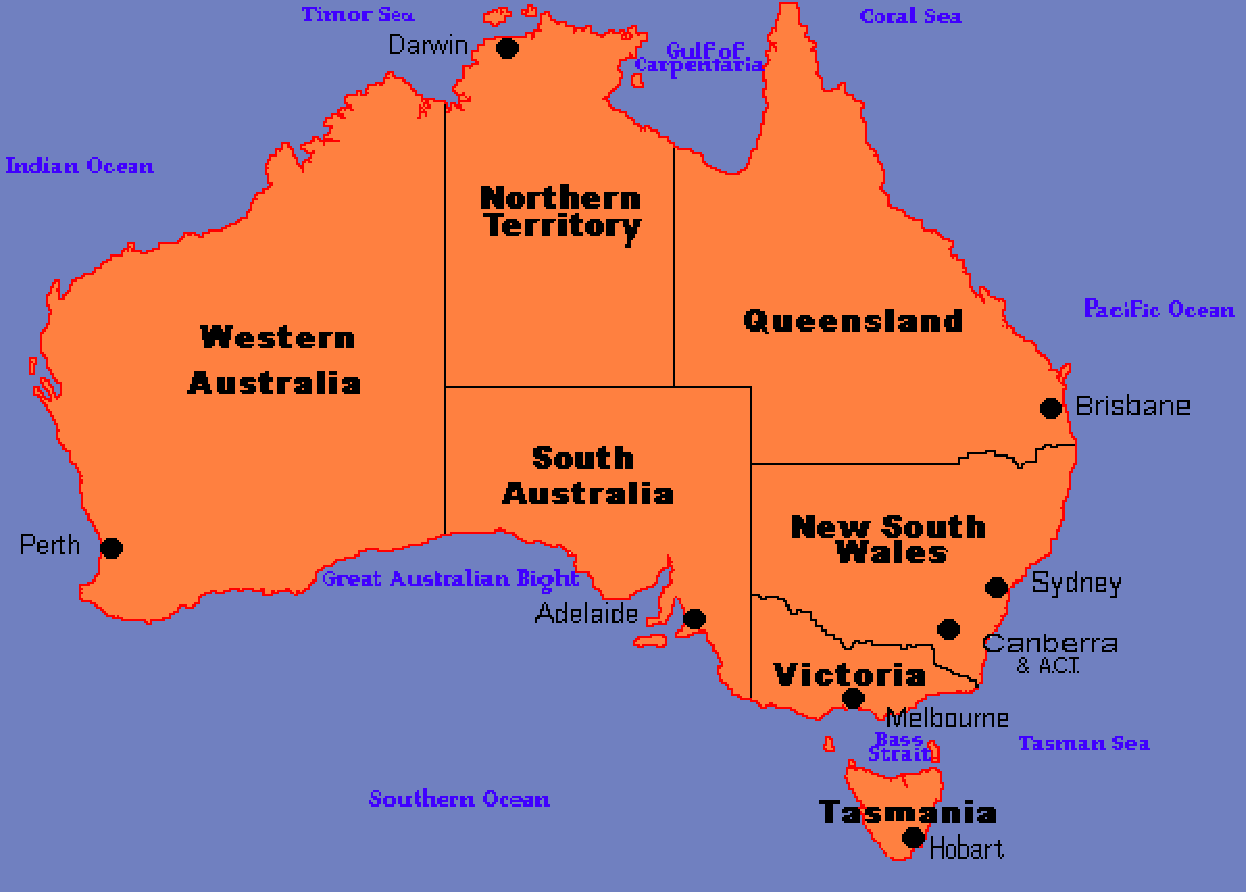
\epsfig{file=Figures/australia.pdf,scale=0.8}} 
  \caption{A map of Australia.}
  \label{fig:australia.pdf}
\end{figure}

\subsection{Example: Map Colouring}
In \href{https://en.wikipedia.org/wiki/Four_color_theorem}{map colouring} a map showing different state
borders is given and the task is to colour the different states such that no two states that have a common
border share the same colour.  \myFig{australia.pdf} shows a map of Australia.  There are seven different
states in Australia:
\begin{enumerate}
\item Western Australia, abbreviated as $\mathrm{WA}$,
\item Northern Territory, abbreviated as $\mathrm{NT}$,
\item South Australia, abbreviated as $\mathrm{SA}$,
\item Queensland, abbreviated as $\mathrm{Q}$,
\item New South Wales, abbreviated as $\mathrm{NSW}$,
\item Victoria, abbreviated as $\mathrm{V}$, and
\item Tasmania, abbreviated as $\mathrm{T}$.
\end{enumerate}
Figure \ref{fig:australia.pdf} would certainly look better if different states had been coloured with different
colours.  For the purpose of 
this example let us assume that we have only three colours available.  The question then is whether it is 
possible to colour the different states in a way that no two neighbouring states share the same colour.  This
problem can be formalized as a constraint satisfaction problem.  To this end we define:
\begin{enumerate}
\item $\texttt{Vars} := \{ \mathtt{WA}, \mathtt{NT}, \mathtt{SA}, \mathtt{Q}, \mathtt{NSW}, \mathtt{V}, \mathtt{T} \}$,
\item $\texttt{Values} := \{ \texttt{red}, \texttt{green}, \texttt{blue} \}$,
\item $\texttt{Constraints} := $ \\[0.1cm]
      \hspace*{0.0cm}
      $\bigl\{ \mathtt{WA} \not= \mathtt{NT}, \mathtt{WA} \not= \mathtt{SA},
                 \mathtt{NT} \not= \mathtt{SA}, \mathtt{NT} \not= \mathtt{Q},
                 \mathtt{SA} \not= \mathtt{Q},  \mathtt{SA} \not= \mathtt{NSW}, \mathtt{SA} \not= \mathtt{V}, 
                 \mathtt{Q}  \not= \mathtt{NSW},
                 \mathtt{NSW}\not= \mathtt{V}, 
                 \mathtt{V}  \not= \mathtt{T}
       \bigr\}
      $
\end{enumerate}
Then $\mathcal{P} := \langle \texttt{Vars}, \texttt{Values}, \texttt{Constraints} \rangle$ is a constraint satisfaction problem.  
If we define the assignment $\mathcal{I}$ such that
\begin{enumerate}
\item $\mathcal{I}(\mathtt{WA}) = \texttt{blue}$,
\item $\mathcal{I}(\mathtt{NT}) = \texttt{red}$,
\item $\mathcal{I}(\mathtt{SA}) = \texttt{green}$,
\item $\mathcal{I}(\mathtt{Q}) = \texttt{blue}$,
\item $\mathcal{I}(\mathtt{NSW}) = \texttt{red}$,
\item $\mathcal{I}(\mathtt{V}) = \texttt{blue}$,
\item $\mathcal{I}(\mathtt{T}) = \texttt{red}$,
\end{enumerate}
then you can check that the assignment $\mathcal{I}$ is indeed a solution to the constraint satisfaction problem $\mathcal{P}$.

\subsection{Example: The Eight Queens Puzzle}
The \href{https://en.wikipedia.org/wiki/Eight_queens_puzzle}{eight queens problem} asks to put 8 queens onto a
chessboard such that no queen can attack another queen.  In \href{https://en.wikipedia.org/wiki/Chess}{chess},
a queen can attack all pieces that are either in the same row, the same column, or the same diagonal.  If we
want to put 8 queens on a chessboard such that no two queens can attack each other, we have to put exactly one
queen in every row:  If we would put more than one queen in a row, the queens in that row can attack each other.
If we would leave a row empty, then, given that the other rows contain at most one queen, there would be less
than 8 queens on the board.  Therefore, in order to model the eight queens problem as a constraint satisfaction
problem, we will use the following set of variables:
\\[0.2cm]
\hspace*{1.3cm}
$\texttt{Vars} := \{ \texttt{Q}_1, \texttt{Q}_2, \texttt{Q}_3, \texttt{Q}_4, \texttt{Q}_5, \texttt{Q}_6, \texttt{Q}_7,\texttt{Q}_8 \}$,
\\[0.2cm]
where for $i \in \{1,\cdots,8\}$ the variable $\texttt{Q}_i$ specifies the column of the queen that is placed in
row $i$.   As the columns run from one to eight, we define the set $\texttt{Values}$ as
\\[0.2cm]
\hspace*{1.3cm}
$\texttt{Values} := \{1,2,3,4,5,6,7,8\}$.
\\[0.2cm]
Next, let us define the constraints.  There are two different types of constraints.
\begin{enumerate}
\item We have constraints that express that no two queens positioned in different rows share the same column.
      To capture these constraints, we define
      \\[0.2cm]
      \hspace*{1.3cm}
      $\texttt{SameRow} := \bigl\{ \texttt{Q}_i \not= \texttt{Q}_j \bigm| i \in \{1,\cdots,8\} \wedge j \in \{1,\cdots,8\} \wedge j < i \bigr\}$.
      \\[0.2cm]
      Here the condition $i < j$ ensures that, for example, we have the constraint $\texttt{Q}_2 \not= \texttt{Q}_1$
      but not the constraint  $\texttt{Q}_1 \not= \texttt{Q}_2$, as the latter constraint would be redundant if
      the former constraint has already been established.
\item We have constraints that express that no two queens positioned in different rows share the same 
      diagonal.  The queens in row $i$ and row $j$ share the same diagonal iff the equation
      \\[0.2cm]
      \hspace*{1.3cm}
      $|i - j| = |\texttt{Q}_i - \texttt{Q}_j|$
      \\[0.2cm]
      holds.  The expression $|i-j|$ is the absolute value of the difference of the rows of the queens in row
      $i$ and row $j$,  while the expression $|\texttt{Q}_i - \texttt{Q}_j|$ is the absolute value of the difference of the
      columns of these queens.  To capture these constraints, we define
      \\[0.2cm]
      \hspace*{1.3cm}
      $\texttt{SameDiagonal} := \bigl\{ |i  - j| \not= |\texttt{Q}_i - \texttt{Q}_j| \bigm| i \in \{1,\cdots,8\} \wedge j \in \{1,\cdots,8\} \wedge j < i \bigr\}$.
\end{enumerate}
Then, the set of constraints is defined as 
\\[0.2cm]
\hspace*{1.3cm}
$\texttt{Constraints} := \texttt{SameRow} \cup \texttt{SameDiagonal}$
\\[0.2cm]
and the eight queens problem can be stated as the constraint satisfaction problem
\\[0.2cm]
\hspace*{1.3cm}
$\mathcal{P} := \langle \texttt{Vars}, \texttt{Values}, \texttt{Constraints} \rangle$.
\\[0.2cm]
If we define the assignment $\mathcal{I}$ such that
\\[0.2cm]
\hspace*{1.3cm}
$\mathcal{I}(\texttt{Q}_1) := 4,\; \mathcal{I}(\texttt{Q}_2) := 8,\; \mathcal{I}(\texttt{Q}_3) := 1,\; \mathcal{I}(\texttt{Q}_4) := 2,\; \mathcal{I}(\texttt{Q}_5) := 6,\; \mathcal{I}(\texttt{Q}_6) := 2,\; \mathcal{I}(\texttt{Q}_7) := 7,\; \mathcal{I}(\texttt{Q}_8) := 5$,
\\[0.2cm]
then it is easy to see that this assignment is a solution of the eight queens problem.  This solution is shown
in \myFig{eight-queens.txt}.


\begin{figure}[!ht]
  \centering
\hspace*{0.0cm}
\vbox{\offinterlineskip
   \hrule height1pt
   \hbox{\vrule width1pt\bigchess
         \vbox{\hbox{0Z0L0Z0Z}
               \hbox{Z0Z0Z0ZQ}
               \hbox{QZ0Z0Z0Z}
               \hbox{Z0L0Z0Z0}
               \hbox{0Z0Z0L0Z}
               \hbox{ZQZ0Z0Z0}
               \hbox{0Z0Z0ZQZ}
               \hbox{Z0Z0L0Z0}}%
         \vrule width1pt}
   \hrule height1pt}

  \caption{A solution of the eight queens problem.}
  \label{fig:eight-queens.txt}
\end{figure}
Later, when we implement procedures to solve  \textsc{Csp}s, we will represent variable assignments and partial
variable assignments as dictionaries.  For example, the variable assignment $\mathcal{I}$ defined above would
then be represented as the dictionary 
\\[0.2cm]
\hspace*{1.3cm}
$\mathcal{I} = \bigl\{ \texttt{Q}_1:4,\, \texttt{Q}_2:8,\, \texttt{Q}_3:1,\, \texttt{Q}_4:3,\, 
             \texttt{Q}_5:6,\, \texttt{Q}_6:2,\, \texttt{Q}_7:7,\, \texttt{Q}_8:5) 
     \bigr\}$.
\\[0.2cm]
If we define 
\\[0.2cm]
\hspace*{1.3cm}
$\mathcal{B} := \bigl\{ \texttt{Q}_1:4,\, \texttt{Q}_2:8,\, \texttt{Q}_3:1) \bigr\}$,
\\[0.2cm]
then $\mathcal{B}$ is a partial assignment and $\texttt{dom}(\mathcal{B}) = \{ \texttt{Q}_1, \texttt{Q}_2, \texttt{Q}_3 \}$.  This
partial assignment is shown in \myFig{eight-queens-partial.txt}.

\begin{figure}[!ht]
  \centering
\hspace*{0.0cm}
\vbox{\offinterlineskip
   \hrule height1pt
   \hbox{\vrule width1pt\bigchess
         \vbox{\hbox{0Z0L0Z0Z}
               \hbox{Z0Z0Z0ZQ}
               \hbox{QZ0Z0Z0Z}
               \hbox{Z0Z0Z0Z0}
               \hbox{0Z0Z0Z0Z}
               \hbox{Z0Z0Z0Z0}
               \hbox{0Z0Z0Z0Z}
               \hbox{Z0Z0Z0Z0}}%
         \vrule width1pt}
   \hrule height1pt}

  \caption{The partial assignment $\bigl\{ \texttt{Q}_1 \mapsto 4, \texttt{Q}_2 \mapsto 8, \texttt{Q}_3 \mapsto 1) \bigr\}$.}
  \label{fig:eight-queens-partial.txt}
\end{figure}



\myFig{queens-csp.stlx} shows a \textsl{Python} program that can be used to create the eight queens puzzle as a
\textsc{Csp}.  

\begin{figure}[!ht]
\centering
\begin{minted}[ frame         = lines, 
                framesep      = 0.3cm, 
                firstnumber   = 1,
                bgcolor       = sepia,
                numbers       = left,
                numbersep     = -0.2cm,
                xleftmargin   = 0.2cm,
                xrightmargin  = 0.2cm,
              ]{python3}
    def queensCSP():
        "Returns a CSP coding the 8 queens problem."
        S            = range(1, 8+1)          # used as indices
        Variables    = [ f'Q{i}' for i in S ]
        Values       = { 1, 2, 3, 4, 5, 6, 7, 8 }
        SameRow      = { f'Q{i} != Q{j}' for i in S for j in S if i < j }
        SameDiagonal = { f'abs(Q{i}-Q{j}) != {j-i}' for i in S for j in S if i < j }
        return (Variables, Values, SameRow | SameDiagonal)
\end{minted}
\vspace*{-0.3cm}
\caption{\textsl{Python} code to create the CSP representing the eight queens puzzle.}
\label{fig:queens-csp.stlx}
\end{figure}


\subsection{A Backtracking Constraint Solver}
One approach to solve a \textsc{Csp} that is both conceptually simple and reasonable efficient is
\blue{backtracking}.  The idea is to try to build variable assignments incrementally:  We start with
an empty dictionary and pick a variable $x_1$ that needs to have a value assigned.  For this variable, we
choose a value $v_1$ and assign it to this variable.  This yields the partial assignment $\{ x_1:v_1 \}$.
Next, we evaluate all those constraints that mention only the variable $x_1$ and check whether these constraints
are satisfied.  If any of these constraints is evaluated as \texttt{False}, we try to assign another value to
$x_1$ until we find a value that satisfies all constraints that mention only $x_1$.

In general, if we have a partial variable assignment $\mathcal{B}$ of the form
\\[0.2cm]
\hspace*{1.3cm}
$\mathcal{B} = \{ x_1:v_1, \cdots, x_k:v_k \}$
\\[0.2cm]
and we already know that all constraints that mention only the variables $x_1$, $\cdots$, $x_k$ are satisfied
by $\mathcal{B}$, then in order to extend $\mathcal{B}$ we pick another variable $x_{k+1}$ and choose a
value $v_{k+1}$ such that all those constraints that mention only the variables  $x_1$, $\cdots$, $x_k$,
$x_{k+1}$ are satisfied.  If we discover that there is no such value $v_{k+1}$, then we have to undo the
assignment $x_k:v_k$ and try to find a new value $v_k$ such that, first, those constraints mentioning only 
the variables  $x_1$, $\cdots$, $x_k$ are satisfied, and, second, it is possible to find a value $v_{k+1}$ that
can be assigned to $x_{k+1}$.  This step of going back and trying to find a new value for the variable $x_k$ is
called \blue{backtracking}.  It might be necessary to backtrack more than one level and to also undo the
assignment of $v_{k-1}$ to $x_{k-1}$ or, indeed, we might be forced to undo the assignments of all variables
$x_i$, $\cdots$, $x_k$ for some $i \in \{1,\cdots, n\}$.  The details of this search procedure are best
explained by looking at its implementation. \myFig{CSP-Solver.ipynb} shows a simple \textsc{Csp} solver that
employs backtracking.  We discuss this program next.

\begin{figure}[!ht]
\centering
\begin{minted}[ frame         = lines, 
                  framesep      = 0.3cm, 
                  firstnumber   = 1,
                  bgcolor       = sepia,
                  numbers       = left,
                  numbersep     = -0.2cm,
                  xleftmargin   = 0.8cm,
                  xrightmargin  = 0.8cm,
                  ]{python3}
    import extractVars as ev
                  
    def solve(CSP):
        "Compute a solution for the given constraint satisfaction problem."
        Variables, Values, Constraints = CSP
        CSP = (Variables,
               Values,
               [(f, ev.extractVars(f) & set(Variables)) for f in Constraints]
              )
        try:
            return backtrack_search({}, CSP)
        except Backtrack:
            return  # no solution found
\end{minted}
\vspace*{-0.3cm}
\caption{A backtracking \textsc{Csp} solver}
\label{fig:CSP-Solver.ipynb}
\end{figure}

\begin{enumerate}
\item As we need to determine the variables occurring in a given constraint, we import the module
      \texttt{extractVar}.  This module implements a function $\texttt{extractVars}(f)$ that takes
      a formula $f$ written as a \textsl{Python} expression and returns the set of all variables occurring in
      $f$. 

\item The procedure $\texttt{solve}$ takes a constraint satisfaction problem $\texttt{CSP}$ as input and tries
      to find a solution.    
      \begin{enumerate}
      \item First, in line 5 the $\texttt{CSP}$ is split into its three components.  However, the first
            component $\texttt{Variables}$ does not have to be a set but rather can also be a list.
            If $\texttt{Variables}$ is a list, then backtracking search will assign these variables 
            in the same order as they appear in this list.  This can improve the efficiency of backtracking
            significantly. 
      \item Next, for every constraint $\texttt{f}$ of the given $\texttt{CSP}$, we compute the set of variables that
            are used in $\texttt{f}$.  This is done using the procedure $\texttt{extractVars}$.
            Of these variables we keep only those variables that also occur in the set $\texttt{Variables}$
            because we assume that any other \textsl{Python} variable occurring in a constraint $f$ has already
            a value assigned to it and can therefore be regarded as a constant.

            The variables occurring in a constraint $\texttt{f}$ are then paired with the constraint $\texttt{f}$ and
            the correspondingly modified data structure is stored in $\texttt{CSP}$ and is called an
            \blue{augmented \textsc{Csp}}.

            The reason to compute and store these variables is efficiency: When we later check whether a constraint $\texttt{f}$
            is satisfied for a partial variable assignment $\texttt{Assignment}$ where $\texttt{Assignment}$ is
            stored as a dictionary, we only need to check the constraint $\texttt{f}$ iff all of the variables occurring
            in $\texttt{f}$ are elements of the domain of $\texttt{Assignment}$.   It would be wasteful to compute
            these variables every time.
      \item Next, we call the function $\texttt{backtrack\_search}$ to compute a solution of $\texttt{CSP}$.
            This function call is enclosed in a \texttt{try}-\texttt{except}-block.
            The function $\texttt{backtrack\_search}$ either returns a solution or, if it is not able to
            find a solution, it throws an exception of class \texttt{Backtrack}.  If this happens,
            the \texttt{except} block silently discards this exception and the procedure \texttt{solve} returns
            without a result.
   \end{enumerate}
 \end{enumerate}

 \begin{figure}[!ht]
\centering
\begin{minted}[ frame         = lines, 
                  framesep      = 0.3cm, 
                  firstnumber   = 1,
                  bgcolor       = sepia,
                  numbers       = left,
                  numbersep     = -0.2cm,
                  xleftmargin   = 0.0cm,
                  xrightmargin  = 0.0cm,
                ]{python3}          
    def backtrack_search(Assignment, CSP):
        """
        Given a partial variable assignment, this function tries to complete this 
        assignment towards a solution of the CSP.
        """
        (Variables, Values, Constraints) = CSP
        if len(Assignment) == len(Variables):
            return Assignment
        var = [x for x in Variables if x not in Assignment][0]
        for value in Values:
            try:
                if isConsistent(var, value, Assignment, Constraints):
                    NewAssign      = Assignment.copy()
                    NewAssign[var] = value
                    return backtrack_search(NewAssign, CSP)
            except Backtrack:
                continue
        # all values have been tried without success, no solution has been found
        raise Backtrack()
    
    class Backtrack(Exception):
        pass
\end{minted}
\vspace*{-0.3cm}
\caption{The function \texttt{backtrack\_search}}
\label{fig:CSP-Solver.ipynb-backtrack_search}
\end{figure}

Next, we discuss the implementation of the procedure $\texttt{backtrack\_search}$ that is shown in
\myFig{CSP-Solver.ipynb-backtrack_search}.  This procedure receives a partial assignment 
$\texttt{Assignment}$ as input together with an augmented $\texttt{CSP}$.  This partial assignment is
\blue{consistent} with $\texttt{CSP}$:  If $\texttt{f}$ is a constraint of $\texttt{CSP}$ such that
all the variables occurring in $\texttt{f}$ are assigned to in $\texttt{Assignment}$, then evaluating
$\texttt{f}$ using $\texttt{Assignment}$ yields $\texttt{True}$.  Initially, this partial assignment is empty
and hence trivially consistent.  The idea is to extend this partial assignment until it is a complete
assignment that satisfies all constraints of the given $\texttt{CSP}$.
\begin{enumerate}
\item First, the augmented $\texttt{CSP}$ is split into its components.
\item Next, if $\texttt{Assignment}$ is already a complete variable assignment, i.e.~if the dictionary
      $\texttt{Assignment}$ has as many elements as there are variables, then the fact that
      $\texttt{Assignment}$ is partially consistent implies that
      it is a solution of the $\texttt{CSP}$ and, therefore, it is returned.
\item Otherwise, we have to extend the partial $\texttt{Assignment}$.  In order to do so, we first have to
      select a variable $\texttt{var}$ that has not yet been assigned a value in $\texttt{Assignment}$ so far.
      We pick the first variable in the list \texttt{Variables} that is yet unassigned.
      This variable is called $\texttt{var}$.
\item Next, we try to assign a $\texttt{value}$ to the selected variable $\texttt{var}$.  After assigning
      a $\texttt{value}$ to $\texttt{var}$, we immediately check whether this assignment would be consistent
      with the constraints using the procedure $\texttt{isConsistent}$.
      If the partial $\texttt{Assignment}$ turns out to be consistent, the partial $\texttt{Assignment}$
      is extended to the new partial assignment \texttt{NewAssign} that satisfies
      \\[0.2cm]
      \hspace*{1.3cm}
      \texttt{NewAssign[var] = value}
      \\[0.2cm]
      and that coincides with $\texttt{Assignment}$ for all variables different from $\texttt{var}$.
      Then, the procedure $\texttt{backtrack\_search}$ is called recursively to complete this new partial assignment.
      If this is successful, the resulting assignment is a solution of the CSP and is returned.  Otherwise,
      the recursive call of $\texttt{backtrack\_search}$ will instead raise an exception.  This exception is muted 
      by the \texttt{try}-\texttt{except}-block that surrounds the recursive call to $\texttt{backtrack\_search}$.  In that case, the
      \texttt{for}-loop generates a new possible $\texttt{value}$ that can be assigned to the variable
      $\texttt{var}$.  If all possible values have been tried and none was successful, the \texttt{for}-loop
      ends and the statement
      \\[0.2cm]
      \hspace*{1.3cm}
      \texttt{raise Backtrack()}
      \\[0.2cm]
      is executed.  This raises an exception that signals that the current partial $\texttt{Assignment}$ can
      not be completed into a solution of the \texttt{CSP}.
      This exception is caught by one of the \texttt{try}-\texttt{except}-blocks that have been encountered previously.
\end{enumerate}


\begin{figure}[!ht]
\centering
\begin{minted}[ frame         = lines, 
                framesep      = 0.3cm, 
                firstnumber   = 1,
                bgcolor       = sepia,
                numbers       = left,
                numbersep     = -0.2cm,
                xleftmargin   = 0.0cm,
                xrightmargin  = 0.0cm,
              ]{python3}  
    def isConsistent(var, value, Assignment, Constraints):
        NewAssign      = Assignment.copy()
        NewAssign[var] = value
        return all(eval(f, NewAssign) for (f, Vs) in Constraints
                                      if var in Vs and Vs <= NewAssign.keys()
                  )
\end{minted}
\vspace*{-0.3cm}
\caption{The procedure \texttt{isConsistent}}
\label{fig:CSP-Solver.ipynb-isConsistent}
\end{figure}

We still need to discuss the implementation of the auxiliary procedure $\texttt{isConsistent}$
shown in \myFig{CSP-Solver.ipynb-isConsistent}.  This procedure takes a variable $\texttt{var}$, a $\texttt{value}$, a partial 
$\texttt{Assignment}$ and a set of $\texttt{Constraints}$.  It is assumed that $\texttt{Assignment}$ is
\blue{partially consistent} with respect to the set $\texttt{Constraints}$, i.e.~for every formula $\texttt{f}$
occurring in $\texttt{Constraints}$ such that
\\[0.2cm]
\hspace*{1.3cm}
$\texttt{vars}(\texttt{f}) \subseteq \texttt{dom}(\texttt{Assignment})$
\\[0.2cm]
holds, the formula $\texttt{f}$ evaluates to $\texttt{True}$ given the $\texttt{Assignment}$.  The purpose of
$\texttt{isConsistent}$ is to check, whether the extended assignment
\\[0.2cm]
\hspace*{1.3cm}
$\texttt{NA} \;\texttt{:=}\;\texttt{Assignment} \cup \{ \pair(\texttt{var}, \texttt{value}) \}$
\\[0.2cm]
that assigns $\texttt{value}$ to the variable $\texttt{var}$ is still partially consistent with $\texttt{Constraints}$. 
To this end, the \texttt{for}-loop iterates over all $\texttt{Formula}$s in $\texttt{Constraints}$. 
However, we only have to check those $\texttt{Formula}$s that contain the variable $\texttt{var}$ and,
furthermore, have the property that
\\[0.2cm]
\hspace*{1.3cm}
$\texttt{Vars}(\texttt{Formula}) \subseteq \texttt{dom}(\texttt{NA})$,
\\[0.2cm]
i.e.~all variables occurring in $\texttt{Formula}$ need to have a value assigned in
$\texttt{NA}$.  The reasoning is as follows:
\begin{enumerate}
\item If $\texttt{var}$ does not occur in $\texttt{Formula}$, then adding $\texttt{var}$ to
      $\texttt{Assignment}$ cannot change the result of evaluating $\texttt{Formula}$ and as
      $\texttt{Assignment}$ is assumed to be partially consistent with respect to $\texttt{Formula}$, 
      $\texttt{NA}$ is also partially consistent with respect to $\texttt{Formula}$.
\item If $\texttt{dom}(\texttt{NA}) \not\subseteq \texttt{Vars}(\texttt{Formula})$, then $\texttt{Formula}$ can not be evaluated anyway. 
\end{enumerate}
If we use backtracking, we can solve the 8 queens problem in less than a second.
For the eight queens puzzle the order in which variables are tried is not particularly important.  The reason
is that all variables are connected to all other variables.  For other problems the ordering of the variables
can be \red{very important}.  The general strategy is that variables that are strongly related to each other should
be grouped together in the list $\texttt{Variables}$.



\section{Normalformen für prädikatenlogische Formeln}
Im nächsten Abschnitt gehen wir daran, einen Kalkül $\vdash$ für die
Prädikaten-Logik zu definieren.  Genau wie im Falle der Aussagen-Logik wird dies wesentlich einfacher, wenn wir
uns auf Formeln, die in einer \blue{Normalform}  vorliegen, beschränken.  Bei dieser Normalform handelt es sich
nun um sogenannte \blue{prädikatenlogische Klauseln}.  Diese werden ähnlich definiert wie in der
Aussagen-Logik:  Ein \blue{prädikatenlogisches Literal} ist eine atomare Formel oder die Negation einer
atomaren Formel.  Eine prädikatenlogische Klausel ist dann eine Disjunktion prädikatenlogischer Literale.
Wir zeigen in diesem Abschnitt, dass jede Formel-Menge $M$
so in eine Menge von prädikatenlogischen Klauseln $K$ transformiert werden kann, dass $M$ genau dann erfüllbar ist, wenn $K$
erfüllbar ist.  Daher ist die Beschränkung auf prädikatenlogische Klauseln keine echte Einschränkung.  Zunächst geben wir einige
Äquivalenzen an, mit deren Hilfe Quantoren manipuliert werden können. 

\begin{Satz}
  Es gelten die folgenden Äquivalenzen:
  \begin{enumerate}
  \item $\models \neg\big(\forall x\colon f\big) \leftrightarrow \big(\exists x\colon \neg f\big)$
  \item $\models \neg\big(\exists x\colon f\big) \leftrightarrow \big(\forall x\colon \neg f\big)$
  \item $\models \forall x\colon f \wedge \forall x\colon g \leftrightarrow \forall x\colon (f \wedge g)$
  \item $\models \exists x\colon f \vee \exists x\colon g \leftrightarrow \exists x\colon (f \vee g)$
  \item $\models \forall x\colon \forall y\colon f \leftrightarrow \forall y\colon  \forall x\colon f$
  \item $\models \exists x\colon \exists y\colon f \leftrightarrow \exists y\colon  \exists x\colon f$
  \item Falls $x$ eine Variable ist, für die $x \not\in \FV(f)$ ist, so haben wir \\[0.2cm]
        \hspace*{1.3cm} $\models  \forall x\colon f \leftrightarrow f$ \quad und \quad
                        $\models  \exists x\colon f \leftrightarrow f$.
  \item Falls $x$ eine Variable ist, für die  $x \not\in \FV(g)$ gilt, so haben wir die folgenden Äquivalenzen:
    \begin{enumerate}
    \item $\models (\forall x\colon f) \vee g \leftrightarrow \forall x\colon (f \vee g)$ \quad und \quad $\models g \vee (\forall x\colon f) \leftrightarrow \forall x\colon (g \vee f)$,
    \item $\models (\exists x\colon f) \wedge g \leftrightarrow \exists x\colon (f \wedge g)$ \quad und \quad $\models g \wedge (\exists x\colon f) \leftrightarrow \exists x\colon (g \wedge f)$.
    \end{enumerate}
  \end{enumerate}
\end{Satz}

Um die Äquivalenzen der letzten Gruppe anwenden zu können, kann es notwendig sein,
gebundene Variablen umzubenennen. Ist $f$ eine prädikatenlogische Formel und sind $x$ und
$y$ zwei Variablen, so bezeichnet $f[x/y]$ die Formel, die aus $f$ dadurch entsteht, dass
jedes Auftreten der Variablen $x$ in $f$ durch $y$ ersetzt wird.  Beispielsweise gilt \\[0.2cm]
\hspace*{1.3cm} $\bigl(\forall u : \exists v : p(u,v)\bigr)[u/z] = \forall z : \exists v : p(z,v)$
\\[0.2cm]
Damit können wir eine letzte Äquivalenz angeben: Ist $f$ eine prädikatenlogische Formel,
ist $x \in BV(f)$ und ist $y$ eine Variable, die in $f$ nicht auftritt, so gilt \\[0.2cm]
\hspace*{1.3cm} $\models f \leftrightarrow f[x/y]$.
\vspace{0.3cm}

Mit Hilfe der oben stehenden Äquivalenzen und der aussagenlogischen Äquivalenzen, die wir schon kennen, können
wir eine Formel so umformen, dass die Quantoren nur noch außen stehen.  Eine solche Formel ist dann in
\blue{pränexer Normalform}.  Wir führen das Verfahren an einem Beispiel vor: Wir zeigen, dass die Formel 
\\[0.2cm]
\hspace*{1.3cm}
$\forall x\colon p(x) \rightarrow \exists x\colon p(x)$ 
\\[0.2cm]
allgemeingültig ist: 
$$ 
\begin{array}{ll}
                 & \forall x\colon p(x) \rightarrow \exists x\colon p(x)  \\
 \Leftrightarrow & \neg \forall x\colon p(x) \vee \exists x\colon p(x)    \\
 \Leftrightarrow & \exists x\colon \neg p(x) \vee \exists x\colon p(x)    \\
 \Leftrightarrow & \exists x\colon \bigl(\neg p(x) \vee p(x)\bigr) \\
 \Leftrightarrow & \exists x\colon \verum                                                  \\
 \Leftrightarrow & \verum                                                  \\
\end{array}
$$
\\[0.2cm]
In diesem Fall haben wir Glück gehabt, dass es uns gelungen ist, die Formel als Tautologie zu
erkennen.  Im Allgemeinen reichen die obigen Umformungen aber nicht aus, um prädikatenlogische
Tautologien erkennen zu können.  Um Formeln noch stärker vereinfachen zu können, 
führen wir einen weiteren Äquivalenz-Begriff ein.  Diesen Begriff wollen wir vorher durch ein Beispiel
motivieren.  Wir betrachten die beiden Formeln 
\\[0.2cm]
\hspace*{1.3cm} $f_1 = \forall x \colon \exists y \colon p(x,y)$ \quad und \quad $f_2 = \forall x \colon
p\bigl(x,s(x)\bigr)$.
\\[0.2cm]
Die beiden Formeln $f_1$ und $f_2$ sind nicht äquivalent, denn sie entstammen noch nicht
einmal der gleichen Signatur: In der Formel $f_2$ wird das Funktions-Zeichen $s$
verwendet, das in der Formel $f_1$ überhaupt nicht auftritt. 
Auch wenn die beiden Formeln $f_1$ und $f_2$ nicht äquivalent sind, so besteht zwischen
ihnen doch die folgende Beziehung:  Ist $\textsl{S}_1$ eine
prädikatenlogische Struktur, in der die Formel $f_1$ gilt:
\\[0.2cm]
\hspace*{1.3cm}
$\mathcal{S}_1 \models f_1$,
\\[0.2cm]
dann können wir diese Struktur zu einer Struktur $\textsl{S}_2$ erweitern, in der die
Formel $f_2$ gilt:
\\[0.2cm]
\hspace*{1.3cm}
$\mathcal{S}_2 \models f_2$.
\\[0.2cm]
Dazu muss lediglich die Interpretation des Funktions-Zeichens $s$ so gewählt werden, dass
für jedes $x$ tatsächlich $p\bigl(x,s(x)\bigr)$ gilt.  Dies ist möglich, denn die Formel $f_1$ sagt ja aus, 
dass wir zu jedem $x$ einen Wert $y$ finden, für den $p(x,y)$ gilt.   Die Funktion $s$ muss also lediglich zu 
jedem $x$ dieses $y$ zurück geben. 



\begin{Definition}[{\color{blue}Skolemisierung}]
  Es sei $\Sigma = \langle \mathcal{V}, \mathcal{F}, \mathcal{P}, \textsl{arity} \rangle$
  eine Signatur.  Ferner sei $f$ eine geschlossene $\Sigma$-Formel der Form \\[0.2cm]
  \hspace*{1.3cm} 
  $f = \forall x_1, \cdots, x_n \colon \exists y \colon g$. \\[0.2cm]
  Dann wählen wir ein \red{neues} $n$-stelliges Funktions-Zeichen $s$, d.h.~wir nehmen ein Zeichen $s$, dass in
  der Signatur $\Sigma$ nicht auftritt und erweitern die Signatur $\Sigma$ zu der Signatur \\[0.2cm]
  \hspace*{1.3cm} 
  $\Sigma' := \Bigl\langle \mathcal{V}, \mathcal{F} \cup \{s\}, \mathcal{P}, \textsl{arity} \cup \bigl\{\pair(s,n)\bigr\} \Bigr\rangle$, \\[0.2cm]
  in der wir $s$ als neues $n$-stelliges Funktions-Zeichen deklarieren.  Anschließend definieren wir die $\Sigma'$-Formel
  $f'$ wie folgt: \\[0.2cm]
  \hspace*{1.3cm} 
  $f' := \mathtt{Skolem}(f) := 
  \forall x_1 \colon \cdots \forall x_n \colon g\bigl[y \mapsto s(x_1,\cdots,x_n)\bigr]$
  \\[0.2cm]
  Hierbei bezeichnet der Ausdruck $g\bigl[y \mapsto s(x_1,\cdots,x_n)\bigr]$ die Formel, die wir aus $g$
  dadurch erhalten, dass wir jedes Auftreten der Variablen $y$ in der Formel $g$ durch den Term
  $s(x_1,\cdots,x_n)$ ersetzen.  Wir sagen, dass die Formel $f'$ aus der Formel $f$
  durch einen \blue{Skolemisierungs-Schritt} hervorgegangen ist. 
  \eox
\end{Definition}

\example
Es $f$ die folgende Formel aus der Gruppen-Theorie:
\\[0.2cm]
\hspace*{1.3cm}
$f := \forall x: \exists y: y * x = 1$. 
\\[0.2cm]
Dann gilt
\\[0.2cm]
\hspace*{1.3cm}
$\mathtt{Skolem}(f) = \forall x : s(x) * x = 1$.  \eox

\noindent
In welchem Sinne sind eine Formel $f$ und eine Formel $f'$, die aus $f$ durch einen 
Skolem\-isierungs-Schritt hervorgegangen sind, äquivalent?  Zur Beantwortung dieser Frage
dient die folgende Definition. 

\begin{Definition}[Erfüllbarkeits-Äquivalenz] \hspace*{1.1cm} 
   Zwei geschlossene Formeln $f$ und $g$ heißen 
   \blue{erfüllbarkeits-äquivalent}
   falls $f$ und $g$ entweder beide erfüllbar oder beide unerfüllbar sind.
   Wenn $f$ und $g$ erfüllbarkeits-äquivalent sind, so schreiben wir \\[0.2cm]
   \hspace*{1.3cm} $f \approx_e g$.
\eox
\end{Definition}

\noindent
\textbf{Beobachtung:}
Falls die Formel $f'$ aus der Formel $f$ durch einen Skolemisierungs-Schritt 
hervorgegangen ist, so sind $f$ und $f'$ erfüllbarkeits-äquivalent, denn wir können jede Struktur
$\mathcal{S}$, in der die Formel $f$ gilt, zu einer Struktur $\mathcal{S}'$ erweitern, in der auch $f'$ gilt.
\eox

Wir können nun ein einfaches Verfahren angeben, um Existenz-Quantoren aus einer Formel
zu eliminieren.  Dieses Verfahren besteht aus zwei Schritten:  Zunächst bringen wir die Formel
in pränexe Normalform. Anschließend können wir die Existenz-Quantoren der Reihe nach durch 
Skolemisierungs-Schritte eliminieren.  Nach dem oben gemachten Bemerkungen ist die resultierende 
Formel zu der ursprünglichen Formel erfüllbarkeits-äquivalent.  Dieses
Verfahren der Eliminierung von Existenz-Quantoren durch die Einführung neuer
Funktions-Zeichen wird als \blue{Skolemisierung} bezeichnet.  Haben wir eine Formel $F$
in pränexe Normalform gebracht und anschließend skolemisiert, so hat das Ergebnis die Gestalt\\[0.2cm]
\hspace*{1.3cm} $\forall x_1, \cdots, x_n: g$ \\[0.2cm]
und in der Formel $g$ treten keine Quantoren mehr auf.  Die Formel $g$ wird auch als die
\blue{Matrix} der obigen Formel bezeichnet.  Wir können nun  $g$ mit Hilfe
der uns aus dem letzten Kapitel bekannten aussagenlogischen
 Äquivalenzen in konjunktive Normalform bringen.  Wir haben dann eine
Formel der Gestalt \\[0.2cm]
\hspace*{1.3cm} $\forall x_1, \cdots, x_n: (k_1 \wedge \cdots \wedge k_m)$. \\[0.2cm]
Dabei sind die $k_i$ Disjunktionen von prädikatenlogischen \blue{Literalen}.  Wenden wir
hier  die Äquivalenz 
\\[0.2cm]
\hspace*{1.3cm}
$\forall x\colon (f_1\wedge f_2) \leftrightarrow (\forall x\colon f_1) \wedge (\forall x\colon f_2)$
\\[0.2cm]
an, so können wir die All-Quantoren auf die einzelnen $k_i$ verteilen und
die resultierende Formel hat die Gestalt \\[0.2cm]
\hspace*{1.3cm} 
$\big(\forall x_1, \cdots, x_n: k_1\big) \wedge \cdots \wedge \big(\forall x_1, \cdots, x_n: k_m\big)$. \\[0.2cm]
Ist eine Formel $F$ in der obigen
Gestalt, so sagen wir, dass $F$ in \blue{prädikatenlogischer Klausel-Normalform} ist und eine
Formel der Gestalt \\[0.2cm]
\hspace*{1.3cm} $\forall x_1, \cdots, x_n: k$, \\[0.2cm]
bei der $k$ eine Disjunktion prädikatenlogischer Literale ist,
bezeichnen wir als \blue{prädikatenlogische Klausel}.  Ist $M$
eine Menge von Formeln deren Erfüllbarkeit wir untersuchen wollen, so können wir nach dem
bisher gezeigten $M$ immer in eine Menge prädikatenlogischer Klauseln umformen.
Da  dann nur noch All-Quantoren vorkommen, können wir hier die  Notation noch vereinfachen,
indem wir vereinbaren, dass alle Formeln implizit allquantifiziert sind, wir lassen also
die All-Quantoren weg.

Wozu sind nun die Umformungen in Skolem-Normalform gut?  Es geht darum, dass wir 
ein Verfahren entwickeln wollen, mit dem es möglich ist für eine prädikatenlogische Formel
$f$ zu zeigen, dass $f$ allgemeingültig ist, dass also \\[0.2cm]
\hspace*{1.3cm} $\models f$ \\[0.2cm]
gilt.  Wir wissen, dass \\[0.2cm]
\hspace*{1.3cm} $\models f$ \quad g.d.w. \quad $\{\neg f\} \models \falsum$ \\[0.2cm]
gilt, denn die Formel $f$ ist genau dann allgemeingültig, wenn es keine Struktur gibt, in
der die Formel $\neg f$ erfüllbar ist. 
 Wir bilden daher zunächst $\neg f$ und formen $\neg f$ in prädikatenlogische
Klausel-Normalform um.  Wir erhalten Klauseln $k_1, \cdots, k_n$, so dass  \\[0.2cm]
\hspace*{1.3cm} $\neg f \approx_e k_1 \wedge \cdots \wedge k_n$ \\[0.2cm]
gilt.  Anschließend versuchen wir,
aus den Klauseln $k_1,\cdots,k_n$ einen Widerspruch herzuleiten: \\[0.2cm]
\hspace*{1.3cm} $\{k_1, \cdots, k_n\} \vdash \falsum$ \\[0.2cm]
Wenn dies gelingt, dann wissen wir, dass die Menge $\{k_1, \cdots, k_n\}$ unerfüllbar ist.
Damit ist auch $\neg f$ unerfüllbar und also ist $f$ allgemeingültig.
Damit wir aus den Klauseln $k_1,\cdots,k_n$ einen Widerspruch herleiten können,
brauchen wir natürlich noch einen Kalkül, der mit prädikatenlogischen Klauseln arbeitet. 
Einen solchen Kalkül werden wir im übernächsten Abschnitt vorstellen.

Um das Verfahren näher zu erläutern demonstrieren wir es an einem Beispiel. 
Wir wollen untersuchen, ob \\[0.2cm]
\hspace*{1.3cm} 
$\models \big(\exists x\colon \forall y\colon  p(x,y)\big) \rightarrow \big(\forall y\colon \exists x\colon p(x,y)\big)$ \\[0.2cm]
gilt.  Wir wissen, dass dies äquivalent dazu ist, dass  \\[0.2cm]
\hspace*{1.3cm} 
$\Big\{ \neg \Big(\big(\exists x\colon \forall y\colon  p(x,y)\big) \rightarrow  \big(\forall y\colon \exists x\colon p(x,y)\big)\Big)\Big\} \models \falsum$ \\[0.2cm]
gilt.  Wir bringen zunächst die negierte Formel in pränexe Normalform. 
$$
\begin{array}{ll}
                  & \neg \Big(\big(\exists x\colon \forall y\colon  p(x,y)\big) \rightarrow \big(\forall y\colon \exists x\colon p(x,y)\big)\Big) \\
  \leftrightarrow & \neg \Big(\neg \big(\exists x\colon \forall y\colon  p(x,y)\big) \vee \big(\forall y\colon \exists x\colon p(x,y)\big)\Big) \\
  \leftrightarrow &                \big(\exists x\colon \forall y\colon  p(x,y)\big) \wedge \neg \big(\forall y\colon \exists x\colon p(x,y)\big) \\
  \leftrightarrow &\big(\exists x\colon \forall y\colon  p(x,y)\big) \wedge  \big(\exists y\colon  \neg \exists x\colon p(x,y)\big) \\
  \leftrightarrow &\big(\exists x\colon \forall y\colon  p(x,y)\big) \wedge  \big(\exists y\colon  \forall x\colon \neg p(x,y)\big) \\
\end{array}
$$
Um an dieser Stelle weitermachen zu können, ist es nötig, die Variablen in dem  zweiten
Glied der Konjunktion umzubenennen.  Wir ersetzen $x$ durch $u$ und $y$ durch $v$ und erhalten
$$
\begin{array}{ll}
                  &\big(\exists x\colon \forall y\colon  p(x,y)\big) \wedge  \big(\exists y\colon  \forall x\colon \neg p(x,y)\big) \\
  \leftrightarrow &\big(\exists x\colon \forall y\colon  p(x,y)\big) \wedge  \big(\exists v\colon  \forall u\colon \neg p(u,v)\big) \\
  \leftrightarrow &\exists v\colon  \Big( \big(\exists x\colon \forall y\colon  p(x,y)\big) \wedge  \big(\forall u\colon \neg p(u,v)\big) \Big)\\
  \leftrightarrow &\exists v\colon  \exists x\colon  \Big( \big(\forall y\colon  p(x,y)\big) \wedge \big(\forall u\colon \neg p(u,v)\big) \Big)\\
  \leftrightarrow &\exists v\colon  \exists x\colon \forall y\colon \Big( p(x,y) \wedge \big(\forall u\colon \neg p(u,v)\big) \Big)\\
  \leftrightarrow &\exists v\colon  \exists x\colon \forall y\colon \forall u\colon \Big( p(x,y) \wedge \neg p(u,v) \Big)\\
\end{array}
$$
An dieser Stelle müssen wir skolemisieren um die Existenz-Quantoren los zu werden. 
Wir führen dazu zwei neue Funktions-Zeichen $s_1$ und $s_2$ ein. 
Dabei gilt $\mathtt{arity}(s_1) = 0$ und $\mathtt{arity}(s_2) = 0$, denn vor den
Existenz-Quantoren stehen keine All-Quantoren.
$$
\begin{array}{ll}
           & \exists v\colon  \exists x\colon \forall y\colon \forall u\colon \Big( p(x,y) \wedge \neg p(u,v) \Big)\\
 \approx_e & \exists x\colon \forall y\colon \forall u\colon \Big( p(x,y) \wedge \neg p(u,s_1) \Big)\\
 \approx_e & \forall y\colon \forall u\colon \Big( p(s_2,y) \wedge \neg p(u,s_1) \Big)\\
\end{array}
$$
Da jetzt nur noch All-Quantoren auftreten, können wir diese auch noch weglassen,
da wir ja vereinbart haben, dass alle freien Variablen implizit allquantifiziert sind.
Damit können wir nun die prädikatenlogische Klausel-Normalform in Mengen-Schreibweise angeben, diese
ist
\\[0.2cm] 
\hspace*{1.3cm}
$M := \Big\{ \big\{ p(s_2,y) \big\}, \big\{\neg p(u,s_1)\big\}\Big\}$.
\\[0.2cm]
Wir zeigen, dass die Menge $M$ widersprüchlich ist.
Dazu betrachten wir zunächst die Klausel $\big\{ p(s_2,y) \big\}$ und setzen in
dieser Klausel für $y$ die Konstante $s_1$ ein.  Damit erhalten wir die Klausel \\[0.2cm]
\hspace*{1.3cm}  $\big\{ p(s_2,s_1) \big\}$. \hspace*{\fill}(1)\\[0.2cm]
Das Ersetzung von $y$ durch $s_1$ begründen wir damit, dass die obige Klausel ja implizit
allquantifiziert ist und wenn etwas für alle $y$ gilt, dann sicher auch für $y = s_1$.

Als nächstes betrachten wir die Klausel $\big\{\neg p(u,s_1)\big\}$.
Hier setzen wir für die Variablen $u$ die Konstante $s_2$ ein und erhalten dann die
Klausel \\[0.2cm]
\hspace*{1.3cm} $\big\{\neg p(s_2,s_1)\big\}$ \hspace*{\fill} (2) \\[0.2cm]
Nun wenden wir auf die Klauseln (1) und (2) die Schnitt-Regel an und finden \\[0.2cm]
\hspace*{1.3cm} 
$\big\{ p(s_2,s_1) \big\}$, \quad$\big\{\neg p(s_2,s_1)\big\}$ \quad $\vdash \quad \{\}$.
\\[0.2cm]
Damit haben wir einen Widerspruch hergeleitet und gezeigt, dass die Menge $M$ unerfüllbar
ist. Damit ist dann auch \\[0.2cm]
\hspace*{1.3cm} 
$\Big\{ \neg \Big(\big(\exists x\colon \forall y\colon  p(x,y)\big) \rightarrow  \big(\forall y\colon \exists x\colon p(x,y)\big)\Big)\Big\}$
\\[0.2cm]
unerfüllbar und folglich gilt \\[0.2cm]
\hspace*{1.3cm} 
$\models \big(\exists x\colon \forall y\colon  p(x,y)\big) \rightarrow  \big(\forall y\colon \exists x\colon p(x,y)\big)$.

\section{Unifikation}
In dem  Beispiel im letzten Abschnitt haben wir die Terme $s_1$ und $s_2$ geraten, die wir für die Variablen
$y$ und $u$ in den Klauseln $\big\{ p(s_2,y) \big\}$ und  $\big\{\neg p(u,s_1)\big\}$
eingesetzt haben.  Wir haben diese Terme mit dem Ziel gewählt, später die Schnitt-Regel
anwenden zu können.  In diesem Abschnitt zeigen wir nun ein Verfahren, mit dessen Hilfe
wir die benötigten Terme ausrechnen können.
Dazu benötigen wir zunächst den Begriff einer \blue{Substitution}.
\begin{Definition}[Substitution]
    Es sei eine Signatur \\[0.2cm]
    \hspace*{1.3cm} $\Sigma = \langle \mathcal{V}, \mathcal{F}, \mathcal{P}, \textsl{arity} \rangle$ \\[0.2cm]
    gegeben.  Eine {\color{blue}$\Sigma$-Substitution} ist eine endliche Menge von Paaren der Form \\[0.2cm]
    \hspace*{1.3cm} $\sigma = \bigl\{ \langle x_1, t_1 \rangle, \cdots, \langle x_n, t_n \rangle \bigr\}$. \\[0.2cm]
    Dabei gilt:
    \begin{enumerate}
    \item $x_i \in \mathcal{V}$, die $x_i$ sind also Variablen.
    \item $t_i \in \mathcal{T}_\Sigma$, die $t_i$ sind also Terme.
    \item Für $i\not=j$ ist $x_i \not= x_j$, die Variablen sind also paarweise verschieden.
    \end{enumerate}
    
    Ist $\sigma = \bigl\{ \langle x_1, t_1 \rangle, \cdots, \langle x_n, t_n \rangle \bigr\}$ eine
    $\Sigma$-Substitution, so schreiben wir  \\[0.2cm]
    \hspace*{1.3cm} $\sigma = \bigl[ x_1 \mapsto t_1, \cdots, x_n \mapsto t_n \bigr]$.  \\[0.2cm]
    Außerdem definieren wir den \blue{Domain} einer Substitution als \\[0.2cm]
    \hspace*{1.3cm} $\textsl{dom}(\sigma) := \{ x_1, \cdots, x_n\}$.
    \\[0.2cm]
    Die Menge aller Substitutionen bezeichnen wir mit \blue{\textsl{Subst}}.
    \eox
\end{Definition}

\noindent
Substitutionen werden für uns dadurch interessant, dass wir sie auf Terme \blue{anwenden} können.  Ist $t$ ein
Term und $\sigma$ eine Substitution, so ist $t\sigma$ der Term, der aus $t$ dadurch entsteht, dass jedes
Vorkommen einer Variablen $x_i$ durch den zugehörigen Term $t_i$ ersetzt wird.  Die formale Definition folgt. 
\begin{Definition}[Anwendung einer Substitution]
\hspace*{\fill} \\
Es sei $t$ ein Term und es sei $\sigma = \bigl[ x_1 \mapsto t_1, \cdots, x_n \mapsto t_n \bigr]$
eine Substitution. Wir definieren die \blue{Anwendung} von $\sigma$ auf $t$ (Schreibweise \blue{$t\sigma$}) durch Induktion über
den Aufbau von $t$: 
\begin{enumerate}
\item Falls $t$ eine Variable ist, gibt es zwei Fälle:
  \begin{enumerate}
  \item $t = x_i$ für ein $i\in\{1,\cdots,n\}$.  Dann definieren wir \quad  $x_i\sigma := t_i$.
  \item $t = y$ mit $y\in\mathcal{V}$, aber $y \not\in \{x_1,\cdots,x_n\}$. Dann definieren wir \quad $y\sigma := y$.
  \end{enumerate}
\item Andernfalls muss $t$ die Form $t= f(s_1,\cdots,s_m)$ haben. Dann können wir $t\sigma$ durch \\[0.2cm]
      \hspace*{1.3cm} $f(s_1, \cdots, s_m)\sigma := f(s_1\sigma, \cdots, s_m\sigma)$. \\[0.2cm]
      definieren, denn nach Induktions-Voraussetzung sind die Ausdrücke $s_i\sigma$ bereits definiert.      
      \eox
\end{enumerate}
\end{Definition}

Genau wie wir Substitutionen auf Terme anwenden können, können wir eine Substitution
auch auf prädikatenlogische Klauseln anwenden.  Dabei werden Prädikats-Zeichen und
Junktoren wie Funktions-Zeichen behandelt.
Wir ersparen uns eine formale Definition und geben stattdessen zunächst einige Beispiele. 
Wir definieren eine Substitution $\sigma$ durch \\[0.2cm]
\hspace*{1.3cm} $\sigma := \big[ x_1 \mapsto c,\; x_2 \mapsto f(d) \big]$. \\[0.2cm]
In den folgenden drei Beispielen demonstrieren wir zunächst, wie eine Substitution
auf einen Term angewendet werden kann.  Im vierten Beispiel wenden wir die Substitution
dann auf eine Klausel an:
\begin{enumerate}
\item $x_3\sigma = x_3$,
\item $f(x_2)\sigma = f\bigl(f(d)\bigr)$,
\item $h(x_1,g(x_2))\sigma = h\bigl(c,g(f(d))\bigr)$.
\item $\bigl\{ p(x_2), q(d,h(x_3,x_1))\bigr\}\sigma = \bigl\{ p(f(d)),\; q(d,h(x_3,c))\bigr\}$.
\end{enumerate}


\noindent
Als nächstes zeigen wir, wie  Substitutionen miteinander verknüpft werden können.
\begin{Definition}[Komposition von Substitutionen] 
    Es seien\\[0.2cm]
    \hspace*{1.3cm}  $\sigma = \big[ x_1 \mapsto s_1, \cdots, x_m \mapsto s_m \big]$ \quad und \quad  $\tau = \big[ y_1 \mapsto t_1, \cdots, y_n \mapsto t_n \big]$ \\[0.2cm]
    zwei Substitutionen mit $\textsl{dom}(\sigma) \cap \textsl{dom}(\tau) = \{\}$. Dann definieren
    wir die \blue{Komposition} $\sigma\tau$ von $\sigma$ und $\tau$ als \\[0.2cm]
    \hspace*{1.3cm} $\sigma\tau := \big[ x_1 \mapsto s_1\tau, \cdots, x_m \mapsto s_m\tau,\; y_1 \mapsto t_1, \cdots, y_n \mapsto t_n \big]$
    \eox
\end{Definition}

\example
Wir führen das obige Beispiel fort und setzen \\[0.2cm]
\hspace*{1.3cm} $\sigma := \big[ x_1 \mapsto c,\; x_2 \mapsto f(x_3) \big]$
                \quad und \quad $\tau := \big[ x_3 \mapsto h(c,c),\; x_4 \mapsto d \big]$. \\[0.2cm]
Dann gilt: \\[0.2cm]
\hspace*{1.3cm} $ \sigma\tau = \big[ x_1 \mapsto c,\; x_2 \mapsto f(h(c,c)),\; x_3 \mapsto h(c,c),\;x_4 \mapsto d \big]$.
\hspace*{\fill} $\Box$
\vspace{0.3cm}

\noindent
Die Definition der Komposition von Substitutionen ist mit dem Ziel gewählt worden, dass
der folgende Satz gilt.
\begin{Satz} \label{satz:komposition}
    Ist $t$ ein Term und sind $\sigma$ und $\tau$ Substitutionen mit 
    $\textsl{dom}(\sigma) \cap \textsl{dom}(\tau) = \{\}$, so gilt \\[0.2cm]
    \hspace*{1.3cm} $(t \sigma)\tau = t (\sigma\tau)$.
    \hspace*{\fill} $\Box$
\end{Satz}
Der Satz kann durch Induktion über den Aufbau des Termes $t$ bewiesen werden.


\begin{Definition}[Syntaktische Gleichung]
Unter einer \blue{syntaktischen Gleichung} verstehen wir in diesem Abschnitt ein Konstrukt der Form
$s \doteq t$, wobei einer der beiden folgenden Fälle vorliegen muss:
\begin{enumerate}
\item $s$ und $t$ sind Terme  oder
\item $s$ und $t$ sind atomare Formeln.
\end{enumerate}
Weiter definieren wir ein \blue{syntaktisches Gleichungs-System} als eine Menge
von syntaktischen Gleichungen.
\eox
\end{Definition}

Was syntaktische Gleichungen angeht, so machen wir keinen Unterschied zwischen Funktions-Zeichen und
Prädikats-Zeichen.   Dieser Ansatz ist deswegen berechtigt, weil wir Prädikate
ja auch als spezielle Funktionen auffassen können, nämlich als solche
Funktionen, die als Ergebnis einen Wahrheitswert aus der Menge  $\mathbb{B}$ zurück geben.

\begin{Definition}[Unifikator]
Eine Substitution $\sigma$ \blue{löst} eine syntaktische Gleichung $s \doteq t$ genau dann, wenn
$s\sigma = t\sigma$ ist, wenn also durch die Anwendung von $\sigma$ auf $s$ und $t$
tatsächlich identische Objekte entstehen.  Ist $E$ ein syntaktisches Gleichungs-System, so 
sagen wir, dass $\sigma$ ein \blue{Unifikator} von $E$ ist wenn $\sigma$ jede
syntaktische Gleichung in $E$ löst. 
\eox
\end{Definition}
Ist $E = \{ s_1 \doteq t_1, \cdots, s_n \doteq t_n \}$ eine syntaktisches Gleichungs-System
und ist $\sigma$ eine Substitution, so definieren wir \\[0.2cm]
\hspace*{1.3cm}  $E\sigma := \{ s_1\sigma \doteq t_1\sigma, \cdots, s_n\sigma \doteq t_n\sigma \}$.
\vspace{0.3cm}

\example
Wir verdeutlichen die bisher eingeführten Begriffe anhand eines Beispiels.  
Wir betrachten die Gleichung \\[0.2cm]
\hspace*{1.3cm} $p(x_1, f(x_4)) \doteq p( x_2, x_3)$ \\[0.2cm]
und definieren die Substitution \\[0.2cm]
\hspace*{1.3cm} $\sigma := \big[ x_1 \mapsto x_2,\; x_3 \mapsto f(x_4) \big]$. \\[0.2cm]
Die Substitution $\sigma$ löst die obige syntaktische Gleichung, denn es gilt \\[0.2cm]
\hspace*{1.3cm} $p(x_1, f(x_4))\sigma = p(x_2, f(x_4))$ \quad und \quad \\[0.2cm]
\hspace*{1.3cm} $p(x_2, x_3)\sigma \;\quad = p(x_2, f(x_4))$.  \eox


Als nächstes entwickeln wir ein Verfahren, mit dessen Hilfe wir von einer vorgegebenen
Menge $E$ von syntaktischen Gleichungen entscheiden können, ob es einen Unifikator $\sigma$ für $E$
gibt.  Das Verfahren, das wir entwickeln werden, wurde von Martelli und Montanari veröffentlicht \cite{martelli:1982}. 
Wir überlegen uns zunächst, in welchen Fällen wir eine syntaktischen Gleichung $s \doteq t$
garantiert nicht lösen können.  Da gibt es zwei Möglichkeiten: Eine syntaktische Gleichung  \\[0.2cm]
\hspace*{1.3cm} $f(s_1,\cdots,s_m) \doteq g(t_1,\cdots, t_n)$ \\[0.2cm]
ist sicher dann nicht durch eine Substitution lösbar, wenn $f$ und $g$ verschiedene
Funktions-Zeichen sind, denn für jede Substitution $\sigma$ gilt ja \\[0.2cm]
\hspace*{1.0cm} $f(s_1,\cdots,s_m)\sigma = f(s_1\sigma,\cdots,s_m\sigma)$ \quad und \quad
                $g(t_1,\cdots, t_n)\sigma = g(t_1\sigma,\cdots,t_n\sigma)$. \\[0.2cm]
Falls $f \not = g$ ist, haben die Terme  $f(s_1,\cdots,s_m)\sigma$ und $g(t_1,\cdots, t_n)\sigma$ verschieden
Funktions-Zeichen und können daher syntaktisch nicht identisch werden.

Die andere Form einer syntaktischen Gleichung, die garantiert unlösbar ist, ist\\[0.2cm]
\hspace*{1.3cm} $x \doteq f(t_1,\cdots,t_n)$  \quad falls $x \in \textsl{Var}\big(f(t_1,\cdots,t_n)\big)$. \\[0.2cm]
Das diese syntaktische Gleichung unlösbar ist liegt daran, dass die rechte Seite immer mindestens ein
Funktions-Zeichen mehr enthält als die linke.  

Mit diesen Vorbemerkungen können wir nun ein Verfahren angeben, mit dessen Hilfe es
möglich ist, Mengen von syntaktischen Gleichungen zu lösen, oder festzustellen, dass es
keine Lösung gibt.  Das Verfahren operiert auf Paaren der Form 
$\langle F, \tau \rangle$.  Dabei ist $F$ ein syntaktisches Gleichungs-System und
$\tau$ ist eine Substitution.  Wir starten das Verfahren mit dem Paar 
$\langle E, [] \rangle$. Hierbei ist $E$ das zu lösende Gleichungs-System und $[]$ ist die leere Substitution.
Das Verfahren arbeitet, indem die im Folgenden
dargestellten Reduktions-Regeln solange angewendet werden, bis entweder feststeht, dass
die Menge der Gleichungen keine Lösung hat, oder aber ein Paar der Form 
$\langle \{\}, \sigma \rangle$ erreicht wird.  In diesem Fall ist $\sigma$ ein
Unifikator der Menge $E$, mit der wir gestartet sind.  Es folgen die Reduktions-Regeln:
\begin{enumerate}
\item Falls $y\in\mathcal{V}$ eine Variable ist, die \underline{\color{red}nicht} in dem Term $t$ auftritt, so
      können wir die folgende Reduktion durchführen: 
      \[ \Big\langle E \cup \big\{ y \doteq t \big\}, \sigma \Big\rangle \quad\leadsto\quad 
         \Big\langle E[y \mapsto t], \sigma\big[ y \mapsto t \big] \Big\rangle 
      \]
      Diese Reduktions-Regel ist folgendermaßen zu lesen: Enthält die zu untersuchende
      Menge von syntaktischen Gleichungen eine Gleichung der Form $y \doteq t$, wobei die
      Variable $y$ nicht in $t$ auftritt, dann können wir diese Gleichung aus der
      gegebenen Menge von Gleichungen entfernen.  Gleichzeitig wird die Substitution
      $\sigma$ in die Substitution $\sigma\big[ y \mapsto t \big]$ transformiert und auf die restlichen syntaktischen Gleichungen
      wird die Substitution $[y \mapsto t]$ angewendet.
\item Wenn die Variable $y$  in dem Term $t$ auftritt, falls also $y \in \textsl{Var}(t)$
      ist und wenn außerdem $t \not= y$ ist, dann hat das Gleichungs-System 
      $E \cup \big\{ y \doteq t \big\}$ \underline{\color{red}keine} Lösung, wir schreiben 
      \\[0.2cm]
      \hspace*{1.3cm}
      $\Big\langle E \cup \big\{ y \doteq t \big\}, \sigma \Big\rangle\;\leadsto\; \Omega$ \quad
      falls $y \in \textsl{Var}(t)$ und $y \not=t$.
\item Falls $y\in\mathcal{V}$ eine Variable ist und $t$ keine Variable ist, so haben wir folgende Reduktions-Regel:
      \[ \Big\langle E \cup \big\{ t \doteq y \big\}, \sigma \Big\rangle \quad\leadsto\quad 
         \Big\langle E \cup \big\{ y \doteq t \big\}, \sigma \Big\rangle.
      \]   
      Diese Regel wird benötigt, um anschließend eine der ersten beiden Regeln anwenden zu
      können.
\item Triviale syntaktische Gleichungen von Variablen können wir einfach weglassen:
      \[ \Big\langle E \cup \big\{ x \doteq x \big\}, \sigma \Big\rangle \quad\leadsto\quad
         \Big\langle E, \sigma \Big\rangle.
      \]   
\item Ist $f$ ein $n$-stelliges Funktions-Zeichen, so gilt 
      \[ \Big\langle E \cup \big\{ f(s_1,\cdots,s_n) \doteq f(t_1,\cdots,t_n) \big\}, \sigma \Big\rangle 
         \;\leadsto\; 
         \Big\langle E \cup \big\{ s_1 \doteq t_1, \cdots, s_n \doteq t_n\}, \sigma \Big\rangle.
      \]   
      Eine syntaktische Gleichung der Form $f(s_1,\cdots,s_n) \doteq f(t_1,\cdots,t_n)$
      wird also ersetzt durch die $n$ syntaktische Gleichungen $s_1 \doteq t_1$, $\cdots$, $s_n \doteq t_n$      .

      Diese Regel ist im übrigen der Grund dafür, dass wir mit Mengen von syntaktischen Gleichungen
      arbeiten müssen, denn auch wenn wir mit nur einer syntaktischen Gleichung starten, kann 
      durch die Anwendung dieser Regel die Zahl der syntaktischen Gleichungen erhöht werden.

      Ein Spezialfall dieser Regel ist 
      \[ \Big\langle E \cup \big\{ c \doteq c \big\}, \sigma \Big\rangle \;\leadsto\; 
         \Big\langle E, \sigma \Big\rangle.
      \]
      Hier steht $c$ für eine Konstante, also ein 0-stelliges Funktions-Zeichen. 
      Triviale Gleichungen über Konstanten können also einfach weggelassen werden.
\item Das Gleichungs-System $E \cup \big\{ f(s_1,\cdots,s_m) \doteq g(t_1,\cdots,t_n) \big\}$
      hat \underline{\color{red}keine} Lösung, falls die Funk\-tions-Zeichen $f$ und $g$ verschieden sind, wir schreiben
      \[ \Big\langle E \cup \big\{ f(s_1,\cdots,s_m) \doteq g(t_1,\cdots,t_n) \big\},
      \sigma \Big\rangle \;\leadsto\; \Omega \qquad \mbox{falls $f \not= g$}. \]
\end{enumerate}
Haben wir ein nicht-leeres Gleichungs-System $E$ gegeben und starten mit dem Paar 
$\langle E, []\rangle$  , so lässt sich immer eine der
obigen Regeln anwenden.  Diese geht solange bis einer der folgenden Fälle eintritt:
\begin{enumerate}
\item Die 2.~oder die 6.~Regel ist anwendbar.  Dann hat das Gleichungs-System $E$ 
      \underline{\color{red}keine} Lösung und als Ergebnis der Unifikation wird $\Omega$ zurück gegeben.
\item Das Paar $\langle E, [] \rangle$ wird reduziert zu einem Paar $\langle \{\}, \sigma\rangle$.
      Dann ist $\sigma$ ein \blue{Unifikator} von $E$.  In diesem Fall schreiben wir $\sigma = \mathtt{mgu}(E)$.
      Falls $E = \{ s \doteq t \}$ ist, schreiben wir auch $\sigma = \mathtt{mgu}(s, t)$.  Die Abkürzung
      $\mathtt{mgu}$ steht hier für {``\blue{most general unifier}''}.
\end{enumerate}

\example
Wir wenden das oben dargestellte Verfahren an, um die syntaktische Gleichung \\[0.2cm]
\hspace*{1.3cm}  $p(x_1, f(x_4)) \doteq p( x_2, x_3)$  \\[0.2cm]
zu lösen.  Wir haben die folgenden Reduktions-Schritte:
$$
\begin{array}{ll}
          &  \big\langle \big\{ p(x_1, f(x_4)) \doteq p( x_2, x_3) \big\}, \big[ \big] \big\rangle \\[0.2cm]
 \leadsto &  \big\langle \big\{ x_1 \doteq x_2, f(x_4) \doteq x_3 \big\}, \big[ \big] \big\rangle \\[0.2cm]
 \leadsto &  \big\langle \big\{ f(x_4) \doteq x_3 \big\}, \big[ x_1 \mapsto x_2 \big] \big\rangle \\[0.2cm]
 \leadsto &  \big\langle \big\{ x_3 \doteq f(x_4) \big\}, \big[ x_1 \mapsto x_2 \big] \big\rangle \\[0.2cm]
 \leadsto &  \big\langle \big\{\big\}, \big[ x_1 \mapsto x_2,\; x_3 \mapsto f(x_4) \big] \big\rangle \\[0.2cm]
\end{array}
$$
In diesem Fall ist das Verfahren also erfolgreich und wir erhalten die Substitution \\[0.2cm]
\hspace*{1.3cm} $\big[ x_1 \mapsto x_2,\; x_3 \mapsto f(x_4) \big]$ \\[0.2cm]
als Lösung der oben gegebenen syntaktischen Gleichung.  \eox

\example
Wir geben ein weiteres Beispiel und betrachten das Gleichungs-System 
\[ E = \big\{ p(h(x_1,c)) \doteq p(x_2),\; q(x_2, d) \doteq q(h(d,c),x_4) \big\} \]
Wir haben folgende Reduktions-Schritte:
$$
\begin{array}{ll}
          & \big\langle \big\{ p(h(x_1,c)) \doteq p(x_2),\; q(x_2, d) \doteq q(h(d,c),x_4) \big\}, \big[ \big] \big\rangle \\[0.2cm]
 \leadsto & \big\langle \big\{ p(h(x_1,c)) \doteq p(x_2),\; x_2 \doteq h(d,c), \; d \doteq x_4 \big\}, \big[ \big] \big\rangle \\[0.2cm]
 \leadsto & \big\langle \big\{ p(h(x_1,c)) \doteq p(x_2),\; x_2 \doteq h(d,c), \; x_4 \doteq d \big\}, \big[ \big] \big\rangle \\[0.2cm]
 \leadsto & \big\langle \big\{ p(h(x_1,c)) \doteq p(x_2),\; x_2 \doteq h(d,c) \big\}, \big[ x_4 \mapsto d \big] \big\rangle \\[0.2cm]
 \leadsto & \big\langle \big\{ p(h(x_1,c)) \doteq p(h(d,c)) \big\}, \big[ x_4 \mapsto d,\; x_2 \mapsto h(d,c) \big] \big\rangle \\[0.2cm]
 \leadsto & \big\langle \big\{ h(x_1,c) \doteq h(d,c) \big\}, \big[ x_4 \mapsto d,\; x_2 \mapsto h(d,c) \big] \big\rangle \\[0.2cm]
 \leadsto & \big\langle \big\{ x_1 \doteq d,\; c \doteq c \big\}, \big[ x_4 \mapsto d,\; x_2 \mapsto h(d,c) \big] \big\rangle \\[0.2cm]
 \leadsto & \big\langle \big\{ x_1 \doteq d,\big\}, \big[ x_4 \mapsto d,\; x_2 \mapsto h(d,c) \big] \big\rangle \\[0.2cm]
 \leadsto & \big\langle \big\{\big\}, \big[ x_4 \mapsto d,\; x_2 \mapsto h(d,c),\; x_1 \mapsto d \big] \big\rangle \\[0.2cm]
\end{array}
$$
Damit haben wir die Substitution  $\big[ x_4 \mapsto d,\; x_2 \mapsto h(d,c),\; x_1 \mapsto d \big]$ als Lösung 
des anfangs gegebenen syn\-tak\-tischen Gleichungs-Systems gefunden.  
\eox




\section{Ein Kalkül für die Prädikatenlogik ohne Gleichheit}
In diesem Abschnitt setzen wir voraus, dass unsere Signatur $\Sigma$ das Gleichheits-Zeichen nicht
verwendet, denn durch diese Einschränkung wird es wesentlich einfacher, einen vollstängen Kalkül für
die Prädikatenlogik einzuführen.  Zwar gibt es auch für den Fall, dass die Signatur $\Sigma$ das
Gleichheits-Zeichen enthält, einen vollständigen Kalkül.  Dieser ist allerdings deutlich
aufwendiger als der Kalkül, den wir gleich einführen werden.

\begin{Definition}[{\color{blue}Resolution}] 
    Es gelte:
    \begin{enumerate}
    \item $k_1$ und $k_2$ sind prädikatenlogische Klauseln,
    \item $p(s_1,\cdots,s_n)$ und $p(t_1,\cdots,t_n)$ sind atomare Formeln,
    \item die syntaktische Gleichung $p(s_1,\cdots,s_n)  \doteq p(t_1,\cdots,t_n)$ ist lösbar mit 
          \\[0.2cm]
          \hspace*{1.3cm}
          $\mu = \mathtt{mgu}\bigl(p(s_1,\cdots,s_n), p(t_1,\cdots,t_n)\bigr)$. 
    \end{enumerate}
     Dann ist 
     \\[0.2cm]
     \hspace*{1.3cm}
     $\schluss{k_1 \cup\{ p(s_1,\cdots,s_n)\} \quad\quad \{\neg p(t_1,\cdots,t_n)\} \cup k_2}{
                 k_1\mu \cup k_2\mu} 
     $
     eine Anwendung der \blue{Resolutions-Regel}.
     \eox
\end{Definition}
Die Resolutions-Regel ist eine Kombination aus der \blue{Substitutions-Regel} und der 
Schnitt-Regel.  Die Substitutions-Regel hat die Form
\\[0.2cm]
\hspace*{1.3cm}
$\schluss{k}{k\sigma}$. 
\\[0.2cm]
Hierbei ist $k$ eine prädikatenlogische Klausel und $\sigma$ ist eine Substitution.
Unter Umständen kann es sein, dass wir vor der Anwendung der Resolutions-Regel 
die Variablen in einer der beiden Klauseln erst umbenennen
müssen bevor wir die Regel anwenden können.  Betrachten wir dazu ein Beispiel.
Die Klausel-Menge 
\[ M = \Bigl\{ \bigl\{ p(x) \bigr\}, \bigl\{ \neg p(f(x)) \bigr\} \Bigr\} \]
ist widersprüchlich.  Wir können die Resolutions-Regel aber nicht unmittelbar anwenden,
denn die syntaktische Gleichung 
\[ p(x) \doteq p(f(x)) \]
ist unlösbar.  Das liegt daran, dass \textbf{zufällig} in beiden Klauseln dieselbe Variable
verwendet wird.  Wenn wir die Variable $x$ in der zweiten Klausel jedoch zu $y$ umbenennen, erhalten
wir die Klausel-Menge 
\[ \Bigl\{ \bigl\{ p(x) \bigr\}, \bigl\{ \neg p(f(y)) \bigr\} \Bigr\}. \]
Hier können wir die Resolutions-Regel anwenden, denn die syntaktische Gleichung 
\[ p(x) \doteq p(f(y)) \]
hat die Lösung $[x \mapsto f(y)]$.  Dann erhalten wir 
\[ \bigl\{ p(x) \bigr\}, \quad \bigl\{ \neg p(f(y)) \bigr\} \quad \vdash \quad \{\}. \]
und haben damit die Inkonsistenz der Klausel-Menge $M$ nachgewiesen.

\noindent
Die Resolutions-Regel alleine ist nicht ausreichend, um aus einer Klausel-Menge $M$, die
inkonsistent ist, in 
jedem Fall die leere Klausel ableiten zu können: Wir brauchen noch eine zweite Regel.
Um das einzusehen, betrachten wir die Klausel-Menge 
\[ M = \Bigl\{ \bigl\{p(f(x),y), p(u,g(v))\bigr\}, 
               \bigl\{\neg p(f(x),y), \neg p(u,g(v))\bigr\} \Bigr\} 
\]
Wir werden gleich zeigen, dass die Menge $M$ widersprüchlich ist.  Man kann nachweisen,
dass mit der Resolutions-Regel alleine ein solcher Nachweis nicht gelingt.
Ein einfacher, aber für die Vorlesung zu aufwendiger Nachweis dieser Behauptung kann
geführt werden, indem wir ausgehend von der Menge $M$ alle möglichen Resolutions-Schritte
durchführen.  Dabei würden wir dann sehen, dass die leere Klausel nie berechnet werden kann.
Wir stellen daher jetzt die
\blue{Faktorisierungs-Regel} vor, mir der wir später zeigen werden, dass $M$ widersprüchlich
ist.


\begin{Definition}[{\color{blue}Faktorisierung}] Es gelte 
  \begin{enumerate}
  \item $k$ ist  eine prädikatenlogische Klausel,
  \item $p(s_1,\cdots,s_n)$ und $p(t_1,\cdots,t_n)$ sind atomare Formeln,
  \item die syntaktische Gleichung $p(s_1,\cdots,s_n)  \doteq p(t_1,\cdots,t_n)$ ist lösbar, 
  \item $\mu = \mathtt{mgu}\bigl(p(s_1,\cdots,s_n), p(t_1,\cdots,t_n)\bigr)$.
  \end{enumerate}
  Dann sind \\[0.3cm]
  \hspace*{0.8cm}
  $\schluss{k \cup \bigl\{p(s_1,\cdots,s_n),\, p(t_1,\cdots,t_n)\bigl\}}{k\mu \cup \bigl\{p(s_1,\cdots,s_n)\mu\bigr\} }$ 
  \quad und \quad
  $\schluss{k \cup \bigl\{ \neg p(s_1,\cdots,s_n),\, \neg p(t_1,\cdots,t_n)\bigl\}}{k\mu \cup \bigl\{\neg p(s_1,\cdots,s_n)\mu\bigr\} }$ 
  \\[0.3cm]
  Anwendungen der \blue{Faktorisierungs-Regel}.
  \eox
\end{Definition}

\noindent
Wir zeigen, wie sich mit Resolutions- und Faktorisierungs-Regel die Widersprüchlichkeit
der Menge $M$ beweisen lässt.
\begin{enumerate}
\item Zunächst wenden wir die Faktorisierungs-Regel auf die erste Klausel an. 
      Dazu berechnen wir den Unifikator 
      \[ \mu = \mathtt{mgu}\bigl(p(f(x),y), p(u,g(v))\bigr) = [y \mapsto g(v), u \mapsto f(x)]. \]
      Damit können wir die Faktorisierungs-Regel anwenden: 
      \[ \bigl\{p(f(x),y), p(u,g(v))\bigr\} \quad \vdash \quad \bigl\{p(f(x),g(v))\bigr\}. \]
\item Jetzt wenden wir die Faktorisierungs-Regel auf die zweite Klausel an.
      Dazu berechnen wir  den Unifikator 
      \[ \mu = \mathtt{mgu}\bigl(\neg p(f(x),y), \neg p(u,g(v))\bigr) = [y \mapsto g(v), u \mapsto f(x)]. 
      \]
      Damit können wir die Faktorisierungs-Regel anwenden: 
      \[ \bigl\{ \neg p(f(x),y), \neg p(u,g(v))\bigr\} \quad \vdash \quad \bigl\{\neg p(f(x),g(v))\bigr\}.
      \]
\item Wir schließen den Beweis mit einer Anwendung der Resolutions-Regel ab.
      Der dabei verwendete Unifikator ist die leere Substitution, es gilt also $\mu = []$.      
      \[ \bigl\{p(f(x),g(v))\bigr\}, \quad \bigl\{\neg p(f(x),g(v))\bigr\} \quad \vdash \quad \{\}. \]
\end{enumerate}
Ist $M$ eine Menge von prädikatenlogischen Klauseln und ist $k$ eine prädikatenlogische
Klausel, die durch Anwendung der Resolutions-Regel und der Faktorisierungs-Regel aus $M$
hergeleitet werden kann, so schreiben wir \\[0.2cm]
\hspace*{1.3cm} $M \vdash k$.
\\[0.2cm]
Dies wird als \blue{$M$ leitet $k$ her} gelesen.

\begin{Definition}[Allabschluss]
  Ist $k$ eine prädikatenlogische Klausel und ist $\{x_1,\cdots,x_n\}$
  die Menge aller Variablen, die in $k$ auftreten, so definieren wir
  den \blue{Allabschluss}  $\forall(k)$  der Klausel k als \\[0.2cm]
  \hspace*{1.3cm} $\forall(k) := \forall x_1\colon \cdots \forall x_n \colon k$. \eox
\end{Definition}

\noindent
Die für uns wesentlichen Eigenschaften des Beweis-Begriffs $M \vdash k$ werden in den folgenden
beiden Sätzen zusammengefasst.
\begin{Satz}[{\color{blue}Korrektheits-Satz}] \hspace*{\fill} \\
    Ist $M = \{k_1,\cdots,k_n\}$ eine Menge von Klauseln und gilt $M \vdash k$, so folgt \\[0.2cm]
    \hspace*{1.3cm} $\models \forall(k_1) \wedge \cdots \wedge \forall(k_n) \rightarrow \forall(k)$. \\[0.2cm]
    Falls also eine Klausel $k$ aus einer Menge $M$ hergeleitet werden kann,
    so ist $k$ tatsächlich eine Folgerung aus $M$. \qed
\end{Satz}

\noindent
Die Umkehrung des obigen Korrektheits-Satzes gilt nur für die leere Klausel.  Sie wurde 1965 von John
A.~Robinson bewiesen \cite{robinson:1965}.
\begin{Satz}[{\color{blue}Widerlegungs-Vollständigkeit} (Robinson, 1965)] \hspace*{\fill} \\
  Ist $M = \{k_1,\cdots,k_n\}$ eine Menge von Klauseln und gilt 
  $\models \forall(k_1) \wedge \cdots \wedge \forall(k_n) \rightarrow \falsum$, so folgt \\[0.2cm]
  \hspace*{1.3cm} $M \vdash \{\}$.
    \qed
\end{Satz}
\noindent
Damit haben wir nun ein Verfahren in der Hand, um für eine gegebene 
prädikatenlogischer Formel $f$ die Frage, ob $\models f$ gilt, untersuchen zu können.
\begin{enumerate}
\item Wir berechnen zunächst die Skolem-Normalform von $\neg f$ und erhalten dabei so etwas wie \\[0.2cm]
      \hspace*{1.3cm} $\neg f \approx_e \forall x_1, \cdots, x_m \colon g$.
\item Anschließend bringen wir die Matrix $g$ in konjunktive Normalform: 
      \[ g \leftrightarrow k_1 \wedge \cdots \wedge k_n. \]
      Daher haben wir nun 
      \[ \neg f \approx_e k_1 \wedge \cdots \wedge k_n \] 
      und es gilt: 
      \[  
          \models f                           \quad \mbox{g.d.w.} \quad
          \{\neg f\} \models \falsum          \quad \mbox{g.d.w.} \quad 
          \{k_1,\cdots,k_n\} \models \falsum.
      \]
\item Nach dem Korrektheits-Satz und dem Satz über die Widerlegungs-Vollständigkeit gilt
      \\[0.2cm]
      \hspace*{1.3cm} 
      $\{k_1,\cdots,k_n\} \models \falsum$ \quad g.d.w. \quad 
      $\{k_1,\cdots,k_n\} \vdash \falsum$. \\[0.2cm]
      Wir versuchen also, nun die Widersprüchlichkeit der Menge $M = \{ k_1, \cdots, k_n \}$  zu zeigen, indem wir
      aus $M$ die leere Klausel ableiten.
      Wenn diese gelingt, haben wir damit die Allgemeingültigkeit der ursprünglich
      gegebenen Formel $f$ gezeigt.
\end{enumerate}

\example
Zum Abschluss demonstrieren wir das skizzierte Verfahren an einem Beispiel.
Wir gehen von folgenden Axiomen aus:
\begin{enumerate}
\item Jeder Drache ist glücklich, wenn alle seine Kinder fliegen können.
\item Rote Drachen können fliegen.
\item Die Kinder eines roten Drachens sind immer rot.
\end{enumerate}
Wie werden zeigen, dass aus diesen Axiomen folgt, dass alle roten Drachen glücklich sind.
Als erstes formalisieren wir die Axiome und die Behauptung in der Prädikatenlogik.
Wir wählen die Signatur \\[0.2cm]
\hspace*{1.3cm}  $\Sigma_\textsl{Drache} := \langle \mathcal{V}, \mathcal{F}, \mathcal{P}, \textsl{arity} \rangle$ 
\\[0.2cm]
wobei die Mengen $\mathcal{V}$, $\mathcal{F}$, $\mathcal{P}$ und \textsl{arity} wie folgt definiert sind:
\begin{enumerate}
\item $\mathcal{V} := \{x,y,z\}$.
\item $\mathcal{F} = \{\}$.
\item $\mathcal{P} := \{ \textsl{rot}, \textsl{fliegt}, \textsl{glücklich}, \textsl{kind} \}$.
\item $\textsl{arity} := \bigl\{ \pair(\textsl{rot},1), \pair(\textsl{fliegt},1),
  \pair(\textsl{glücklich},1), \pair(\textsl{kind},2)\bigr\}$
\end{enumerate}
Das Prädikat  $\textsl{kind}(x,y)$ soll genau dann wahr sein, wenn $x$ ein Kind von $y$ ist.
Formalisieren wir die Axiome und die Behauptung, so erhalten wir die folgenden
Formeln $f_1, \cdots, f_4$:
\begin{enumerate}
\item $f_1 := \forall x: \Bigl(\forall y: \big(\textsl{kind}(y,x) \rightarrow \textsl{fliegt}(y)\big) \rightarrow \textsl{glücklich}(x)\Bigr)$
\item $f_2 := \forall x: \bigl(\textsl{rot}(x) \rightarrow \textsl{fliegt}(x)\bigr)$
\item $f_3 := \forall x: \bigl(\textsl{rot}(x) \rightarrow \forall y:\bigl( \textsl{kind}(y,x) \rightarrow \textsl{rot}(y)\bigr)\bigr)$
\item $f_4 := \forall x: \bigl(\textsl{rot}(x) \rightarrow \textsl{glücklich}(x)\bigr)$
\end{enumerate}
Wir wollen zeigen, dass die Formel 
\\[0.2cm]
\hspace*{1.3cm} 
$f := f_1 \wedge f_2 \wedge f_3 \rightarrow f_4$ 
\\[0.2cm]
allgemeingültig ist.  Wir betrachten also die Formel $\neg f$ und stellen fest \\[0.2cm]
\hspace*{1.3cm} $\neg f \leftrightarrow f_1 \wedge f_2 \wedge f_3 \wedge \neg f_4$. \\[0.2cm]
Als nächstes müssen wir diese Formel in eine Menge von Klauseln umformen.
Da es sich hier um eine Konjunktion mehrerer Formeln handelt, können wir 
die einzelnen Formeln 
 $f_1$, $f_2$, $f_3$ und  $\neg f_4$  getrennt in Klauseln umwandeln.
\begin{enumerate}
\item Die Formel $f_1$ kann wie folgt umgeformt werden:
 $$ 
  \begin{array}{lcl}
    f_1 & =           & \forall x:\Bigl(\forall y: \big(\textsl{kind}(y,x)
    \rightarrow \textsl{fliegt}(y)\big) \rightarrow \textsl{glücklich}(x) \Bigr) \\[0.2cm]
    &\leftrightarrow & \forall x: \Bigl(\neg \forall y: \big( \textsl{kind}(y,x) \rightarrow \textsl{fliegt}(y)\big) \vee \textsl{glücklich}(x) \Bigr)\\[0.2cm]
    &\leftrightarrow & \forall x: \Bigl(\neg \forall y: \big( \neg \textsl{kind}(y,x) \vee \textsl{fliegt}(y)\big) \vee \textsl{glücklich}(x) \Bigr)\\[0.2cm]
    &\leftrightarrow & \forall x: \Bigl(\exists y: \neg \big( \neg \textsl{kind}(y,x) \vee \textsl{fliegt}(y)\big) \vee \textsl{glücklich}(x) \Bigr)\\[0.2cm]
    &\leftrightarrow & \forall x: \Bigl( \exists y: \big(\textsl{kind}(y,x) \wedge \neg  \textsl{fliegt}(y)\big) \vee \textsl{glücklich}(x) \Bigr)\\[0.2cm]
    &\leftrightarrow & \forall x:  \exists y: \Bigl(\big( \textsl{kind}(y,x) \wedge \neg  \textsl{fliegt}(y)\big) \vee \textsl{glücklich}(x) \Bigr)\\[0.2cm]
    &\approx_e & \forall x: \Bigl(\big( \textsl{kind}(s(x),x) \wedge \neg  \textsl{fliegt}(s(x))\big) \vee \textsl{glücklich}(x) \Bigr)\\
  \end{array}
     $$
      Im letzten Schritt haben wir dabei die Skolem-Funktion $s$ mit 
      $\textsl{arity}(s) = 1$ eingeführt.  Anschaulich berechnet diese Funktion für jeden
      Drachen $x$, der nicht glücklich ist, ein Kind $s(x)$, das nicht fliegen kann.
      Wenn wir in der Matrix dieser Formel das ``$\vee$'' noch ausmultiplizieren, so
      erhalten wir die beiden Klauseln 
      \\[0.2cm]
      \hspace*{1.3cm} $k_1 := \bigl\{ \textsl{kind}(s(x),x), \textsl{glücklich}(x) \bigl\}$,   \\[0.2cm]
      \hspace*{1.3cm} $k_2 := \bigl\{ \neg \textsl{fliegt}(s(x)), \textsl{glücklich}(x) \bigl\}$. 
\item Analog finden wir für $f_2$:
 $$
        \begin{array}{lcl}
            f_2 & =  & \forall x: \bigl(\textsl{rot}(x) \rightarrow \textsl{fliegt}(x) \bigr) \\[0.2cm]
            & \leftrightarrow  & \forall x: \bigl(\neg \textsl{rot}(x) \vee \textsl{fliegt}(x) \bigr)
        \end{array}
      $$ 
      Damit ist $f_2$ zu folgender Klauseln äquivalent: \\[0.2cm]
      \hspace*{1.3cm} $k_3 := \bigl\{ \neg \textsl{rot}(x), \textsl{fliegt}(x) \bigl\}$.
\item Für $f_3$ sehen wir:
 $$
        \begin{array}{lcl}
          f_3 & =          & \forall x: \Bigl(\textsl{rot}(x) \rightarrow 
                             \forall y: \bigl(\textsl{kind}(y,x) \rightarrow \textsl{rot}(y)\bigr) \Bigr) 
          \\[0.2cm]
          &\leftrightarrow & \forall x: \Bigl(\neg \textsl{rot}(x) \vee 
                             \forall y: \bigl(\neg \textsl{kind}(y,x) \vee \textsl{rot}(y)\bigr)\Bigr) 
          \\[0.2cm]
          &\leftrightarrow & \forall x: \forall y: \bigl(\neg \textsl{rot}(x) \vee \neg \textsl{kind}(y,x) \vee \textsl{rot}(y)\bigr)
        \end{array}
      $$
     Das liefert die folgende Klausel: \\[0.2cm]
     \hspace*{1.3cm} $ k_4 := \bigl\{ \neg \textsl{rot}(x), \neg \textsl{kind}(y,x), \textsl{rot}(y)\bigl\}$.
\item Umformung der Negation von $f_4$ liefert:
 $$
        \begin{array}{lcl}
\neg f_4 & =      & \neg \forall x: \bigl(\textsl{rot}(x) \rightarrow \textsl{glücklich}(x)\bigr) 
         \\[0.2cm]
         & \leftrightarrow & \neg \forall x: \bigl(\neg \textsl{rot}(x) \vee \textsl{glücklich}(x) \bigr)
         \\[0.2cm]
         & \leftrightarrow & \exists x: \neg \bigl(\neg \textsl{rot}(x) \vee \textsl{glücklich}(x) \bigr)
         \\[0.2cm]
         & \leftrightarrow & \exists x: \bigl(\textsl{rot}(x) \wedge \neg \textsl{glücklich}(x) \bigr)
         \\[0.2cm]
         & \approx_e & \textsl{rot}(d) \wedge \neg \textsl{glücklich}(d) \\
        \end{array}
      $$
      Die hier eingeführte Skolem-Konstante $d$ steht für einen unglücklichen roten Drachen.
      Das führt zu den Klauseln \\[0.2cm]
      \hspace*{1.3cm} $k_5 = \bigl\{ \textsl{rot}(d) \bigl\}$, \\[0.2cm]
      \hspace*{1.3cm} $k_6 = \bigl\{ \neg \textsl{glücklich}(d) \bigl\}$.
\end{enumerate}
Wir müssen also untersuchen, ob die Menge $M$, die aus den folgenden Klauseln besteht,
widersprüchlich ist: 
\begin{enumerate}
\item $k_1 = \bigl\{ \textsl{kind}(s(x),x),\; \textsl{glücklich}(x) \bigl\}$  
\item $k_2 = \bigl\{ \neg \textsl{fliegt}(s(x)),\; \textsl{glücklich}(x) \bigl\}$
\item $k_3 = \bigl\{ \neg \textsl{rot}(x),\; \textsl{fliegt}(x) \bigl\}$
\item $k_4 = \bigl\{ \neg \textsl{rot}(x),\; \neg \textsl{kind}(y,x),\; \textsl{rot}(y) \bigl\}$
\item $k_5 = \bigl\{ \textsl{rot}(d) \bigl\}$ 
\item $k_6 = \bigl\{ \neg \textsl{glücklich}(d) \bigl\}$
\end{enumerate}
Sei also $M := \bigl\{k_1,k_2,k_3,k_4,k_5,k_6\bigl\}$.
Wir  zeigen, dass $M \vdash \falsum$ gilt:
\begin{enumerate}
\item Es gilt 
      \\[0.2cm]
      \hspace*{1.3cm}
      $\mathtt{mgu}\bigl(\textsl{rot}(d), \textsl{rot}(x)\bigr) = [x \mapsto d]$.
      \\[0.2cm]
      Daher können wir die Resolutions-Regel auf die Klauseln $k_5$ und $k_4$ wie folgt anwenden:
      \\[0.2cm]
      \hspace*{1.3cm}
      $\bigl\{\textsl{rot}(d)\bigl\}$, \ $\bigl\{\neg \textsl{rot}(x), \neg \textsl{kind}(y,x),
       \textsl{rot}(y)\bigl\}$ \ $\vdash$ \ $\bigl\{\neg \textsl{kind}(y,d), \textsl{rot}(y)\bigl\}$.
\item Wir wenden nun auf die resultierende Klausel und auf die Klausel $k_1$ die
      Resolutions-Regel an.  Dazu berechnen wir zunächst
      \\[0.2cm]
      \hspace*{1.3cm}
      $\mathtt{mgu}\bigl(\textsl{kind}(y,d), \textsl{kind}(s(x),x)\bigr) = 
       [y \mapsto s(d), x \mapsto d]$.
      \\[0.2cm]
      Dann haben wir
      \\[0.2cm]
      \hspace*{1.3cm}
       $\bigl\{\neg \textsl{kind}(y,d), \textsl{rot}(y)\bigl\}$, \ 
       $\bigl\{\textsl{kind}(s(x),x), \textsl{glücklich}(x)\bigl\}$ \ $\vdash$ \ 
       $\bigl\{\textsl{glücklich}(d), \textsl{rot}(s(d))\bigl\}$.
\item Jetzt wenden wir auf die eben abgeleitete Klausel und die Klausel $k_6$ die
      Resolutions-Regel an.  Wir haben:
      \\[0.2cm]
      \hspace*{1.3cm}
      $\mathtt{mgu}\bigl(\textsl{glücklich}(d), \textsl{glücklich}(d)\bigr) = []$
      \\[0.2cm]
      Also erhalten wir
      \\[0.2cm]
      \hspace*{1.3cm}
      $\bigl\{\textsl{glücklich}(d), \textsl{rot}(s(d))\bigl\}$, \ $\bigl\{\neg \textsl{glücklich}(d)\bigl\}$ \ $\vdash$ \ $\bigl\{\textsl{rot}(s(d))\bigl\}$.
\item Auf die Klausel $\bigl\{\textsl{rot}(s(d))\bigl\}$ und die Klausel $k_3$ wenden wir
      die Resolutions-Regel an.  Zunächst haben wir
      \\[0.2cm]
      \hspace*{1.3cm}
      $\mathtt{mgu}\bigl(\textsl{rot}(s(d)), \neg \textsl{rot}(x)\bigr) = [x \mapsto s(d)]$
      \\[0.2cm]
      Also liefert die Anwendung der Resolutions-Regel:
      \\[0.2cm]
      \hspace*{1.3cm}
      $\bigl\{\textsl{rot}(s(d))\bigl\}$, \ $\bigl\{\neg \textsl{rot}(x), \textsl{fliegt}(x)\bigl\}$ \ $\vdash$ \ $\bigl\{\textsl{fliegt}(s(d))\bigl\}$
\item Um die so erhaltenen Klausel $\bigl\{\textsl{fliegt}(s(d))\bigl\}$ mit der Klausel
      $k_3$ resolvieren zu können, berechnen wir
      \\[0.2cm]
      \hspace*{1.3cm}
      $\mathtt{mgu}\bigl(\textsl{fliegt}(s(d)), \textsl{fliegt}(s(x))\bigr) = [x \mapsto d]$
      \\[0.2cm]
      Dann liefert die Resolutions-Regel
      \\[0.2cm]
      \hspace*{1.3cm}
      $\bigl\{\textsl{fliegt}(s(d))\bigl\}$, \ $\bigl\{\neg \textsl{fliegt}(s(x)), \textsl{glücklich}(x)\bigl\}$ \ $\vdash$ \ $\bigl\{\textsl{glücklich}(d)\bigl\}$.
\item Auf das Ergebnis $\bigl\{\textsl{glücklich}(d)\bigl\}$ und die Klausel $k_6$ können
      wir nun die Resolutions-Regel anwenden:
      \\[0.2cm]
      \hspace*{1.3cm}
      $\bigl\{\textsl{glücklich}(d)\bigl\}$, \  $\bigl\{\neg \textsl{glücklich}(d)\bigl\}$ \ $\vdash$ \ $\bigl\{\bigl\}$.
\end{enumerate}
Da wir im letzten Schritt die leere Klausel erhalten haben,  ist insgesamt $M \vdash
\falsum$ 
nachgewiesen worden und damit haben wir gezeigt, dass alle kommunistischen Drachen glücklich sind. 
\eox

\exercise
Die von Bertrant Russell definierte \emph{Russell-Menge} $R$ ist
definiert als die Menge aller der Mengen, die sich nicht selbst enthalten.   Damit gilt also
\\[0.2cm]
\hspace*{1.3cm}
$\forall x: \bigl( x \el R \leftrightarrow \neg x \el x)$.
\\[0.2cm]
Zeigen Sie mit Hilfe des in diesem Abschnitt definierten Kalküls, dass diese Formel
widersprüchlich ist. 
\vspace{0.3cm}

\exercise
Gegeben seien folgende Axiome:
\begin{enumerate}
\item Jeder Barbier rasiert alle Personen, die sich nicht selbst rasieren.
\item Kein Barbier rasiert jemanden, der sich selbst rasiert.
\end{enumerate}
Zeigen Sie, dass aus diesen Axiomen logisch die folgende Aussage folgt: \\[0.3cm]
\hspace*{1.3cm} Alle Barbiere sind blond.

\section{\textsl{Prover9} und \textsl{Mace4}}
Der im letzten Abschnitt beschriebene Kalkül lässt sich automatisieren und bildet die Grundlage moderner
automatischer Beweiser.  Gleichzeitig lässt sich auch die Suche nach Gegenbeispielen automatisieren.
Wir stellen in diesem Abschnitt zwei Systeme vor, die diesen Zwecken dienen.
\begin{enumerate}
\item \textsl{Prover9} dient dazu, automatisch prädikatenlogische Formeln zu beweisen.
\item \textsl{Mace4} untersucht, ob eine gegebene Menge prädikatenlogischer Formeln in einer endlichen
  Struktur erfüllbar ist.  Gegebenenfalls wird diese Struktur berechnet.
\end{enumerate}
Die beiden Programme \textsl{Prover9} und \textsl{Mace4} wurden von William McCune \cite{mccune:2010} 
entwickelt, stehen unter der \href{http://www.gnu.org/licenses/gpl.html}{GPL} (\emph{Gnu General
  Public Licence}) und können unter der Adresse 
\\[0.2cm]
\hspace*{1.3cm}
\href{http://www.cs.unm.edu/~mccune/prover9/download/}{\texttt{http://www.cs.unm.edu/\symbol{126}mccune/prover9/download/}}
\\[0.2cm]
im Quelltext heruntergeladen werden.  Wir diskutieren zunächst \textsl{Prover9} und schauen uns anschließend
\textsl{Mace4} an.

\subsection{Der automatische Beweiser \textsl{Prover9}}
\textsl{Prover9} ist ein Programm, das als Eingabe zwei Mengen von Formeln bekommt.  Die erste Menge von
Formeln wird als Menge von \emph{Axiomen} interpretiert, die zweite Menge von Formeln sind die zu
beweisenden \emph{Thereme}, die aus den Axiomen gefolgert werden sollen.  Wollen wir beispielsweise zeigen,
dass in der Gruppen-Theorie aus der Existenz eines  links-inversen Elements auch die Existenz eines
rechts-inversen Elements folgt und dass außerdem das links-neutrale Element auch rechts-neutral ist,
so können wir zunächst die Gruppen-Theorie wie folgt axiomatisieren:
\begin{enumerate}
\item $\forall x: e \cdot x = x$,
\item $\forall x: \exists y: y \cdot x = e$,
\item $\forall x: \forall y: \forall z: (x \cdot y) \cdot z = x \cdot (y \cdot z)$.
\end{enumerate}
Wir müssen nun zeigen, dass aus diesen Axiomen die beiden Formeln
\\[0.2cm]
\hspace*{1.3cm}
$\forall x: x \cdot e = x$ \quad und \quad $\forall x: \exists y: y \cdot x = e$ 
\\[0.2cm]
logisch folgen.  Wir können diese Formeln wie in Abbildung \ref{fig:group2.in} auf Seite
\pageref{fig:group2.in} gezeigt für \textsl{Prover9} darstellen.
Der Anfang der Axiome wird in dieser Datei durch ``\texttt{formulas(sos)}'' eingeleitet und durch
das Schlüsselwort ``\texttt{end\_of\_list}'' beendet.  Zu beachten ist, dass sowohl die Schlüsselwörter als
auch die einzelnen Formel jeweils durch einen Punkt ``\texttt{.}'' beendet werden.  Die Axiome in den Zeilen
2, 3, und 4 drücken aus, dass 
\begin{enumerate}
\item \texttt{e} ein links-neutrales Element ist,
\item zu jedem Element $x$ ein links-inverses Element $y$ existiert und
\item das Assoziativ-Gesetz gilt.
\end{enumerate}
Aus diesen Axiomen folgt, dass das \texttt{e} auch ein rechts-neutrales Element ist und dass außerdem zu
jedem Element $x$ ein rechts-neutrales Element $y$ existiert.  Diese beiden  Formeln sind die zu beweisenden 
\blue{Ziele} und werden in der Datei durch ``\texttt{formulas}(goal)'' markiert.
Trägt die in Abbildung \ref{fig:group2.in} gezeigte Datei den Namen ``\texttt{group2.in}'', so können wir das
Programm \textsl{Prover9} mit dem Befehl 
\\[0.2cm]
\hspace*{1.3cm}
\texttt{prover9 -f group2.in}
\\[0.2cm]
starten und erhalten als Ergebnis die Information, dass die beiden in Zeile 8 und 9 gezeigten Formeln
tatsächlich aus den vorher angegebenen Axiomen folgen.  Ist eine Formel nicht beweisbar, so gibt es zwei Möglichkeiten:
In bestimmten Fällen kann \textsl{Prover9} tatsächlich erkennen, dass ein Beweis unmöglich ist.  In
diesem Fall bricht das Programm die Suche nach einem Beweis mit einer entsprechenden Meldung ab.
Wenn die Dinge ungünstig liegen, ist es auf Grund der Unentscheidbarkeit der Prädikatenlogik nicht
möglich zu erkennen, dass die Suche nach einem Beweis scheitern muss.  In einem solchen Fall
läuft das Programm solange weiter, bis kein freier Speicher mehr zur Verfügung steht und
bricht dann mit einer Fehlermeldung ab.


\begin{figure}[!ht]
\centering
\begin{Verbatim}[ frame         = lines, 
                  framesep      = 0.3cm, 
                  firstnumber   = 1,
                  labelposition = bottomline,
                  numbers       = left,
                  numbersep     = -0.2cm,
                  xleftmargin   = 0.8cm,
                  xrightmargin  = 0.8cm,
                ]
    formulas(sos).
    all x (e * x = x).                              % left neutral 
    all x exists y (y * x = e).                     % left inverse
    all x all y all z ((x * y) * z = x * (y * z)).  % associativity
    end_of_list.
    
    formulas(goals).
    all x (x * e = x).                              % right neutral 
    all x exists y (x * y = e).                     % right inverse
    end_of_list.
\end{Verbatim}
\vspace*{-0.3cm}
\caption{Textuelle Darstellung der Axiome der Gruppentheorie.}
\label{fig:group2.in}
\end{figure}


\textsl{Prover9} versucht, einen indirekten Beweis zu führen.  Zunächst werden die Axiome in
prädikatenlogische Klauseln 
überführt. Dann wird jedes zu beweisenden Theorem negiert und die negierte Formel wird ebenfalls in 
Klauseln überführt.  Anschließend versucht \textsl{Prover9} aus der Menge aller Axiome zusammen mit den
Klauseln, die sich aus der Negation eines der zu beweisenden Theoreme ergeben, die leere
Klausel herzuleiten.  Gelingt dies, so ist bewiesen, dass das jeweilige  Theorem tatsächlich aus den Axiomen
folgt.   Abbildung \ref{fig:group-commutative.in} zeigt eine
Eingabe-Datei für \textsl{Prover9}, bei der versucht wird, das Kommutativ-Gesetz aus den Axiomen der
Gruppentheorie zu folgern.  Der Beweis-Versuch mit \textsl{Prover9} schlägt allerdings fehl.  In diesem Fall
wird die Beweissuche nicht endlos fortgesetzt.  Dies liegt daran, dass es \textsl{Prover9} gelingt, in
endlicher Zeit alle aus den gegebenen Voraussetzungen folgenden Formeln abzuleiten.
Leider ist ein solcher Fall eher die Ausnahme als die Regel.

\begin{figure}[!ht]
\centering
\begin{Verbatim}[ frame         = lines, 
                  framesep      = 0.3cm, 
                  firstnumber   = 1,
                  labelposition = bottomline,
                  numbers       = left,
                  numbersep     = -0.2cm,
                  xleftmargin   = 0.8cm,
                  xrightmargin  = 0.8cm,
                ]
    formulas(sos).
    all x (e * x = x).                              % left neutral 
    all x exists y (y * x = e).                     % left inverse
    all x all y all z ((x * y) * z = x * (y * z)).  % associativity
    end_of_list.
    
    formulas(goals).
    all x all y (x * y = y * x).                    % * is commutative
    end_of_list.
\end{Verbatim}
\vspace*{-0.3cm}
\caption{Gilt das Kommutativ-Gesetz in allen Gruppen?}
\label{fig:group-commutative.in}
\end{figure}


\subsection{\textsl{Mace4} }
Dauert ein Beweisversuch  mit \textsl{Prover9} endlos, so ist zunächst nicht klar, ob das zu beweisende
Theorem gilt.  Um sicher zu sein, 
dass eine Formel nicht aus einer gegebenen Menge von Axiomen folgt, reicht es aus, eine Struktur zu
konstruieren, in der alle Axiome erfüllt sind, in der das zu beweisende Theorem aber falsch ist.
Das Programm \textsl{Mace4} dient genau dazu, solche Strukturen zu finden.  Das funktioniert natürlich nur,
solange die Strukturen endlich sind.  Abbildung \ref{fig:group.in} zeigt eine Eingabe-Datei, mit deren Hilfe
wir die Frage, ob es endliche nicht-kommutative Gruppen gibt, unter Verwendung von \textsl{Mace4} beantworten
können.  In den Zeilen 2, 3 und 4 stehen die Axiome der Gruppen-Theorie.  Die Formel in Zeile 5 postuliert,
dass für die beiden Elemente $a$ und $b$ das Kommutativ-Gesetz nicht gilt, dass also $a \cdot b \not= b \cdot
a$ ist.  Ist der in 
Abbildung \ref{fig:group.in} gezeigte Text in einer Datei mit dem Namen ``\textsl{group.in}'' gespeichert, so
können wir \textsl{Mace4} durch das Kommando
\\[0.2cm]
\hspace*{1.3cm}
\textsl{mace4 -f group.in}
\\[0.2cm]
starten.  \textsl{Mace4} sucht für alle positiven natürlichen  Zahlen $n=1,2,3,\cdots$, ob es eine Struktur 
$\mathcal{S} = \langle \mathcal{U}, \mathcal{J} \rangle$ mit $\textsl{card}(U) = n$ gibt, in der die
angegebenen Formeln gelten.  Bei $n=6$ wird \textsl{Mace4} fündig und berechnet tatsächlich eine Gruppe mit 6
Elementen, in der das Kommutativ-Gesetz verletzt ist.

\begin{figure}[!ht]
\centering
\begin{Verbatim}[ frame         = lines, 
                  framesep      = 0.3cm, 
                  firstnumber   = 1,
                  labelposition = bottomline,
                  numbers       = left,
                  numbersep     = -0.2cm,
                  xleftmargin   = 0.8cm,
                  xrightmargin  = 0.8cm,
                ]
    formulas(theory).
    all x (e * x = x).                              % left neutral
    all x exists y (y * x = e).                     % left inverse
    all x all y all z ((x * y) * z = x * (y * z)).  % associativity
    a * b != b * a.                                 % a and b do not commute
    end_of_list.
\end{Verbatim}
\vspace*{-0.3cm}
\caption{Gibt es eine Gruppe, in der das Kommutativ-Gesetz nicht gilt?}
\label{fig:group.in}
\end{figure}


Abbildung \ref{fig:group.out} zeigt einen Teil der von \textsl{Mace4} produzierten Ausgabe.
Die Elemente der Gruppe sind die Zahlen $0, \cdots, 5$, die Konstante $a$ ist das Element $0$,
$b$ ist das Element $1$, $e$ ist das Element $2$.  Weiter sehen wir, dass das Inverse von $0$ wieder $0$ ist,
das Inverse von $1$ ist $1$ das Inverse von $2$ ist $2$, das Inverse von $3$ ist $4$, das Inverse von $4$ ist
$3$ und das Inverse von $5$ ist $5$.  Die Multiplikation wird durch die folgende Gruppen-Tafel realisiert:
\\[0.2cm]
\hspace*{1.3cm}
\hspace*{1.3cm}
\begin{tabular}[t]{|l||l|l|l|l|l|l|}
\hline
$\circ$ & 0 & 1 & 2 & 3 & 4 & 5 \\
\hline
\hline
      0 & 2 & 3 & 0 & 1 & 5 & 4 \\
\hline
      1 & 4 & 2 & 1 & 5 & 0 & 3 \\
\hline
      2 & 0 & 1 & 2 & 3 & 4 & 5 \\
\hline
      3 & 5 & 0 & 3 & 4 & 2 & 1 \\
\hline
      4 & 1 & 5 & 4 & 2 & 3 & 0 \\
\hline
      5 & 3 & 4 & 5 & 0 & 1 & 2 \\
\hline
\end{tabular}
\\[0.2cm]
Diese Gruppen-Tafel zeigt, dass
\\[0.2cm]
\hspace*{1.3cm}
$a \circ b = 0 \circ 1 = 3$, \quad aber \quad
$b \circ a = 1 \circ 0 = 4$
\\[0.2cm]
gilt, mithin ist das Kommutativ-Gesetz tatsächlich verletzt.

\begin{figure}[!ht]
\centering
\begin{Verbatim}[ frame         = lines, 
                  framesep      = 0.3cm, 
                  firstnumber   = 1,
                  labelposition = bottomline,
                  numbers       = left,
                  numbersep     = -0.2cm,
                  xleftmargin   = 0.5cm,
                  xrightmargin  = 0.5cm,
                ]
    ============================== DOMAIN SIZE 6 =========================
    
    === Mace4 starting on domain size 6. ===
    
    ============================== MODEL =================================
    
    interpretation( 6, [number=1, seconds=0], [
    
            function(a, [ 0 ]),
    
            function(b, [ 1 ]),
    
            function(e, [ 2 ]),
    
            function(f1(_), [ 0, 1, 2, 4, 3, 5 ]),
    
            function(*(_,_), [
    			   2, 3, 0, 1, 5, 4,
    			   4, 2, 1, 5, 0, 3,
    			   0, 1, 2, 3, 4, 5,
    			   5, 0, 3, 4, 2, 1,
    			   1, 5, 4, 2, 3, 0,
    			   3, 4, 5, 0, 1, 2 ])
    ]).
    
    ============================== end of model ==========================
\end{Verbatim}
\vspace*{-0.3cm}
\caption{Ausgabe von \textsl{Mace4}.}
\label{fig:group.out}
\end{figure}

\remark
Der Theorem-Beweiser \textsl{Prover9} ist ein Nachfolger des Theorem-Beweisers \textsl{Otter}.  Mit Hilfe von
\textsl{Otter} ist es William McCune 1996 gelungen, die Robbin'sche Vermutung zu beweisen \cite{mccune:1997}.
Dieser Beweis war damals sogar der \href{http://www.nytimes.com/}{New York Times} eine Schlagzeile wert,
nachzulesen unter
\\[0.2cm]
\hspace*{1.3cm}
\href{http://www.nytimes.com/library/cyber/week/1210math.html}{\texttt{http://www.nytimes.com/library/cyber/week/1210math.html}}.
\\[0.2cm]
Dies zeigt, dass \href{https://en.wikipedia.org/wiki/Automated_theorem_proving}{automatische Theorem-Beweiser}
durchaus nützliche Werkzeuge sein können.  Nichtsdestoweniger ist die Prädikatenlogik unentscheidbar und bisher
sind  nur wenige offene mathematische Probleme mit Hilfe von automatischen Beweisern gelöst worden.  Das wird
sich vermutlich auch in der näheren Zukunft nicht ändern.  \eox

\section{Reflexion}
\begin{enumerate}
\item Was ist eine \blue{Signatur}?
\item Wie haben wir die Menge $\mathcal{T}_\Sigma$ der \blue{$\Sigma$-Terme} definiert?
\item Was ist eine \blue{atomare} Formel?
\item Wie haben wir die Menge $\mathbb{F}_\Sigma$ der \blue{$\Sigma$-Formeln} definiert?
\item Was ist eine \blue{$\Sigma$-Struktur}?
\item Es sei $\mathcal{S}$ eine  $\Sigma$-Struktur.  Wie haben wir den Begriff der
      \blue{$\mathcal{S}$-Variablen-Belegung} definiert?
\item Wie haben wir die Semantik von $\Sigma$-Formeln definiert?
\item Wann ist eine prädikatenlogische Formel \blue{allgemeingültig}?
\item Was bedeutet die Schreibweise \blue{$\mathcal{S} \models F$} für eine $\Sigma$-Struktur $\mathcal{S}$ und eine
      $\Sigma$-Formel $F$?
\item Wann ist eine Menge von prädikatenlogischen Formeln \blue{unerfüllbar}?
\item Was ist ein \blue{Constraint Satisfaction Problem}?
\item Wie funktioniert \blue{Backtracking}?
\item Warum kommt es beim Backtracking auf die Reihenfolge an, in der die verschiedenen Variablen instantiiert
      werden?
\item Was sind \blue{prädikatenlogische Klauseln} und welche Schritte müssen wir durchführen, um eine gegebene
      prädikatenlogische Formel in eine erfüllbarkeits-äquivalente Menge von Klauseln zu überführen?
\item Was ist eine \blue{Substitution}?
\item Was ist ein \blue{Unifikator}?
\item Geben Sie die Regeln von \blue{Martelli und Montanari} an!
\item Wie ist die \blue{Resolutions-Regel} definiert und warum ist es eventuell erforderlich, Variablen umzubenennen,
      bevor die Resolutions-Regel angewendet werden kann?
\item Was ist die \blue{Faktorisierungs-Regel}?
\item Wie gehen wir vor, wenn wir die Allgemeingültigkeit einer prädikatenlogischen Formel $f$ nachweisen wollen?
\end{enumerate}

%%% Local Variables: 
%%% mode: latex
%%% TeX-master: "logic"
%%% ispell-local-dictionary: "deutsch8"
%%% End: 


\bibliographystyle{alpha}
\bibliography{cs}

\end{document}



%%% Local Variables: 
%%% mode: latex
%%% TeX-master: "logic"
%%% End: 
